\cleartoleftpage{}
\begin{figure}[p]
  \begingroup
  \centering
  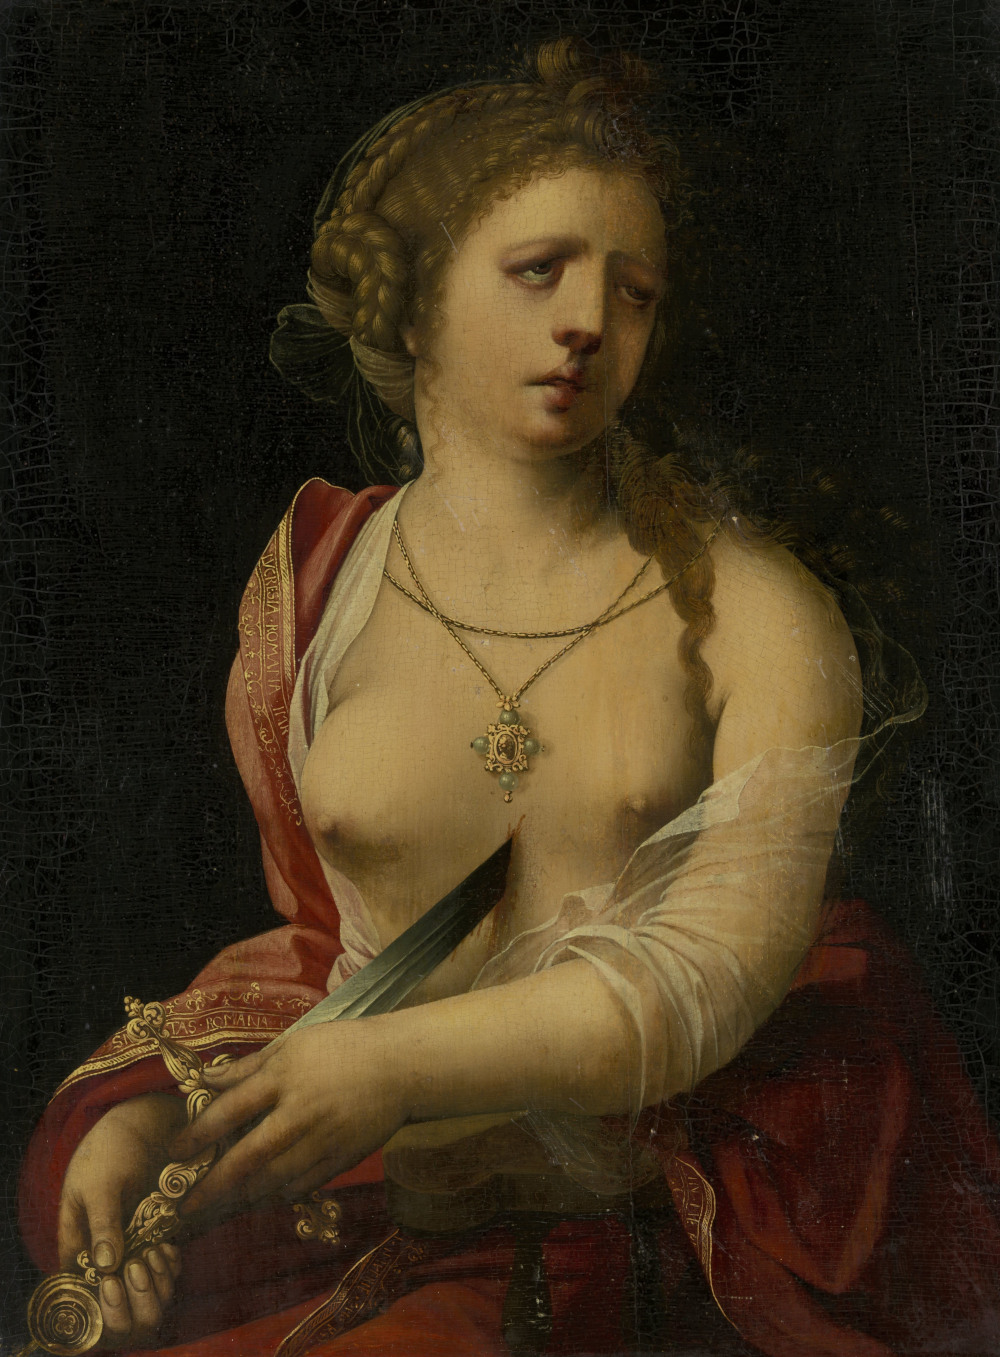
\includegraphics[keepaspectratio,width=\textwidth]{figures/suicide-of-lucretia-small.jpg}
  \captionart{SuicideofLucretia}
  \label{fig:suicideoflucretia}
\end{figure}
% Force float here
\clearpage{}
\thispagestyle{titleontop}
\chapter{Cure of Melancholy in General}
{
%THE SECOND PARTITION. THE CURE OF MELANCHOLY. THE FIRST SECTION, MEMBER, SUBSECTION.
%PART. II SECT. I MEMB. I SUBSECT. I
\section{Unlawful Cures rejected.}
\lettrine[lines=3]{I}{nveterate} Melancholy, howsoever it may seem to be a continuate,
inexorable disease, hard to be cured, accompanying them to their
graves, most part, as Montanus observes\authorfootnote{2789}, yet many times it may be
helped, even that which is most violent, or at least, according to the
same author\authorfootnote{2790}, it may be mitigated and much eased. Nil desperandum.
It may be hard to cure, but not impossible for him that is most
grievously affected, if he but willing to be helped.

Upon this good hope I will proceed, using the same method in the cure,
which I have formerly used in the rehearsing of the causes; first
general, then particular; and those according to their several species.
Of these cures some be lawful, some again unlawful, which though
frequent, familiar, and often used, yet justly censured, and to be
controverted. As first, whether by these diabolical means, which are
commonly practised by the devil and his ministers, sorcerers, witches,
magicians, \etc{}, by spells, cabilistical words, charms, characters,
images, amulets, ligatures, philters, incantations, \etc{}, this disease
and the like may be cured? and if they may, whether it be lawful to
make use of them, those magnetical cures, or for our good to seek after
such means in any case? The first, whether they can do any such cures,
is questioned amongst many writers, some affirming, some denying.
Valesius, cont. med. lib. 5. cap. 6. Malleus Maleficar, Heurnius, lib.
3. pract. med. cap. 28. Caelius lib. 16. c. 16. Delrio Tom. 3. Wierus
lib. 2. de praestig. daem. Libanius Lavater de spect. part. 2. cap. 7.
Holbrenner the Lutheran in Pistorium, Polydore Virg. l. 1. de prodig.
Tandlerus, Lemnius, (Hippocrates and Avicenna amongst the rest) deny
that spirits or devils have any power over us, and refer all with
Pomponatius of Padua to natural causes and humours. Of the other
opinion are Bodinus Daemonamantiae, lib. 3, cap. 2. Arnoldus, Marcellus
Empyricus, I. Pistorius, Paracelsus Apodix. Magic. Agrippa lib. 2. de
occult. Philos. cap. 36. 69. 71. 72. et l. 3, c. 23, et 10. Marcilius
Ficinus de vit. coelit. compar. cap. 13. 15. 18. 21. \etc{} Galeottus de
promiscua doct. cap. 24. Jovianus Pontanus Tom. 2. Plin. lib. 28, c. 2.
Strabo, lib. 15. Geog. Leo Suavius: Goclenius de ung. armar. Oswoldus
Crollius, Ernestus Burgravius, Dr. Flud, \etc{} Cardan de subt. brings
many proofs out of Ars Notoria, and Solomon's decayed works, old
Hermes, Artefius, Costaben Luca, Picatrix, \etc{} that such cures may be
done. They can make fire it shall not burn, fetch back thieves or
stolen goods, show their absent faces in a glass, make serpents lie
still, stanch blood, salve gouts, epilepsies, biting of mad dogs,
toothache, melancholy, et omnia mundi mala, make men immortal, young
again as the \authorfootnote{2791}Spanish marquis is said to have done by one of his
slaves, and some, which jugglers in \authorfootnote{2792}China maintain still (as
Tragaltius writes) that they can do by their extraordinary skill in
physic, and some of our modern chemists by their strange limbecks, by
their spells, philosopher's stones and charms. \authorfootnote{2793}Many doubt, saith
Nicholas Taurellus, whether the devil can cure such diseases he hath
not made, and some flatly deny it, howsoever common experience confirms
to our astonishment, that magicians can work such feats, and that the
devil without impediment can penetrate through all the parts of our
bodies, and cure such maladies by means to us unknown. Daneus in his
tract de Sortiariis subscribes to this of Taurellus; Erastus de lamiis,
maintaineth as much, and so do most divines, out of their excellent
knowledge and long experience they can commit \authorfootnote{2794}agentes cum
patientibus, colligere semina rerum, eaque materiae applicare, as
Austin infers de Civ. Dei et de Trinit. lib. 3. cap. 7. et 8. they can
work stupendous and admirable conclusions; we see the effects only, but
not the causes of them. Nothing so familiar as to hear of such cures.

Sorcerers are too common; cunning men, wizards, and white-witches, as
they call them, in every village, which if they be sought unto, will
help almost all infirmities of body and mind, Servatores in Latin, and
they have commonly St. Catherine's wheel printed in the roof of their
mouth, or in some other part about them, resistunt incantatorum
praestigiis (\authorfootnote{2795}Boissardus writes) morbos a sagis motos propulsant
\etc{}, that to doubt of it any longer, \authorfootnote{2796}or not to believe, were to
run into that other sceptical extreme of incredulity, saith Taurellus.

Leo Suavius in his comment upon Paracelsus seems to make it an art,
which ought to be approved; Pistorius and others stiffly maintain the
use of charms, words, characters, \etc{}. Ars vera est, sed pauci artifices
reperiuntur; the art is true, but there be but a few that have skill in
it. Marcellius Donatus lib. 2. de hist, mir. cap. 1. proves out of
Josephus' eight books of antiquities, that \authorfootnote{2797}Solomon so cured all
the diseases of the mind by spells, charms, and drove away devils, and
that Eleazer did as much before Vespasian. Langius in his med. epist.
holds Jupiter Menecrates, that did so many stupendous cures in his
time, to have used this art, and that he was no other than a magician.

Many famous cures are daily done in this kind, the devil is an expert
physician, as Godelman calls him, lib. 1. cap. 18. and God permits
oftentimes these witches and magicians to produce such effects, as
Lavater cap. 3. lib. 8. part. 3. cap. 1. Polid. Virg. lib. 1. de
prodigiis, Delrio and others admit. Such cures may be done, and as
Paracels. Tom. 4. de morb. ament. stiffly maintains, \authorfootnote{2798}they cannot
otherwise be cured but by spells, seals, and spiritual physic.

\authorfootnote{2799}Arnoldus, lib. de sigillis, sets down the making of them, so doth
Rulandus and many others.

\latininlinetrans{this being granded}{Hoc posito}, they can effect such cures, the main question is, whether
it be lawful in a desperate case to crave their help, or ask a wizard's
advice. 'Tis a common practice of some men to go first to a witch, and
then to a physician, if one cannot the other shall, Flectere si
nequeant superos Acheronta movebunt. \authorfootnote{2800}It matters not, saith
Paracelsus, whether it be God or the devil, angels, or unclean spirits
cure him, so that he be eased. If a man fall into a ditch, as he
prosecutes it, what matter is it whether a friend or an enemy help him
out? and if I be troubled with such a malady, what care I whether the
devil himself, or any of his ministers by God's permission, redeem me?
He calls a \authorfootnote{2801} magician, God's minister and his vicar, applying that
of vos estis dii profanely to them, for which he is lashed by T.
Erastus part. 1. fol. 45. And elsewhere he encourageth his patients to
have a good faith, \authorfootnote{2802} a strong imagination, and they shall find the
effects: let divines say to the contrary what they will. He proves and
contends that many diseases cannot otherwise be cured. Incantatione
orti incantatione curari debent; if they be caused by incantation,
\authorfootnote{2803}they must be cured by incantation. Constantinus lib. 4. approves
of such remedies: Bartolus the lawyer, Peter Aerodius rerum Judic. lib.
3. tit. 7. Salicetus Godefridus, with others of that sect, allow of
them; modo sint ad sanitatem quae a magis fiunt, secus non, so they be
for the parties good, or not at all. But these men are confuted by
Remigius, Bodinus, daem. lib. 3. cap 2. Godelmanus lib. 1. cap. 8,
Wierus, Delrio lib. 6. quaest. 2. tom. 3. mag. inquis. Erastus de
Lamiis; all our \authorfootnote{2804}divines, schoolmen, and such as write cases of
conscience are against it, the scripture itself absolutely forbids it
as a mortal sin, Levit. cap. \rn{xviii.} \rn{xix.} \rn{xx.} Deut. \rn{xviii.} \etc{}. Rom.
\rn{viii.} 19. Evil is not to be done, that good may come of it. Much better
it were for such patients that are so troubled, to endure a little
misery in this life, than to hazard their souls' health for ever, and
as Delrio counselleth, \authorfootnote{2805}much better die, than be so cured. Some
take upon them to expel devils by natural remedies, and magical
exorcisms, which they seem to approve out of the practice of the
primitive church, as that above cited of Josephus, Eleazer, Irenaeus,
Tertullian, Austin. Eusebius makes mention of such, and magic itself
hath been publicly professed in some universities, as of old in
Salamanca in Spain, and Krakow in Poland: but condemned anno 1318, by
the chancellor and university of \authorfootnote{2806}Paris. Our pontifical writers
retain many of these adjurations and forms of exorcisms still in the
church; besides those in baptism used, they exorcise meats, and such as
are possessed, as they hold, in Christ's name. Read Hieron. Mengus cap.
3. Pet. Tyreus, part. 3. cap. 8. What exorcisms they prescribe, besides
those ordinary means of \authorfootnote{2807}fire suffumigations, lights, cutting the
air with swords, cap. 57. herbs, odours: of which Tostatus treats, 2.
Reg. cap. 16. quaest. 43, you shall find many vain and frivolous
superstitious forms of exorcisms among them, not to be tolerated, or
endured.

%MEMB. II.

\section{Lawful Cures, first from God.}

\lettrine{B}{eing} so clearly evinced, as it is, all unlawful cures are to be
refused, it remains to treat of such as are to be admitted, and those
are commonly such which God hath appointed, \authorfootnote{2808}by virtue of stones,
herbs, plants, meats, and the like, which are prepared and applied to
our use, by art and industry of physicians, who are the dispensers of
such treasures for our good, and to be \authorfootnote{2809}honoured for necessities'
sake, God's intermediate ministers, to whom in our infirmities we are
to seek for help. Yet not so that we rely too much, or wholly upon
them: a Jove principium, we must first begin with \authorfootnote{2810}prayer, and
then use physic; not one without the other, but both together. To pray
alone, and reject ordinary means, is to do like him in Aesop, that when
his cart was stalled, lay flat on his back, and cried aloud help
Hercules, but that was to little purpose, except as his friend advised
him, rotis tute ipse annitaris, he whipped his horses withal, and put
his shoulder to the wheel. God works by means, as Christ cured the
blind man with clay and spittle: Orandum est ut sit mens sana in
corpore sano. As we must pray for health of body and mind, so we must
use our utmost endeavours to preserve and continue it. Some kind of
devils are not cast out but by fasting and prayer, and both necessarily
required, not one without the other. For all the physic we can use,
art, excellent industry, is to no purpose without calling upon God, nil
juvat immensos Cratero promittere montes: it is in vain to seek for
help, run, ride, except God bless us.
\authorfootnote{2811}---non Siculi dapes
Dulcem elaborabunt saporem.
Non animum cytheraeve cantus.

\authorfootnote{2812}Non domus et fundus, non aeris acervus et auri
Aegroto possunt domino deducere febres.

\authorfootnote{2813}With house, with land, with money, and with gold,
The master's fever will not be controll'd.

We must use our prayer and physic both together: and so no doubt but
our prayers will be available, and our physic take effect. 'Tis that
Hezekiah practised, 2 King. \rn{xx.} Luke the Evangelist: and which we are
enjoined, Coloss. IV. not the patient only, but the physician himself.
Hippocrates, a heathen, required this in a good practitioner, and so
did Galen, lib. de Plat. et Hipp. dog. lib. 9. cap. 15. and in that
tract of his, an mores sequantur temp. cor. ca. 11. 'tis a rule which
he doth inculcate, \authorfootnote{2814} and many others. Hyperius in his first book
de sacr. script. lect. speaking of that happiness and good success
which all physicians desire and hope for in their cures, \authorfootnote{2815}tells
them that it is not to be expected, except with a true faith they call
upon God, and teach their patients to do the like. The council of
Lateran, Canon 22. decreed they should do so: the fathers of the church
have still advised as much: whatsoever thou takest in hand (saith
\authorfootnote{2816}Gregory) let God be of thy counsel, consult with him; that
healeth those that are broken in heart, (Psal. \rn{cxlvii.} 3.) and bindeth
up their sores. Otherwise as the prophet Jeremiah, cap. \rn{xlvi.} 11.
denounced to Egypt, In vain shalt thou use many medicines, for thou
shalt have no health. It is the same counsel which \authorfootnote{2817}Comineus that
politic historiographer gives to all Christian princes, upon occasion
of that unhappy overthrow of Charles Duke of Burgundy, by means of
which he was extremely melancholy, and sick to death: insomuch that
neither physic nor persuasion could do him any good, perceiving his
preposterous error belike, adviseth all great men in such cases,
\authorfootnote{2818}to pray first to God with all submission and penitency, to
confess their sins, and then to use physic. The very same fault it was,
which the prophet reprehends in Asa king of Judah, that he relied more
on physic than on God, and by all means would have him to amend it. And
'tis a fit caution to be observed of all other sorts of men. The
prophet David was so observant of this precept, that in his greatest
misery and vexation of mind, he put this rule first in practice. Psal.
\rn{lxxvii.} 3. When I am in heaviness, I will think on God. Psal. \rn{lxxxvi.}
4. Comfort the soul of thy servant, for unto thee I lift up my soul:
and verse 7. In the day of trouble will I call upon thee, for thou
hearest me. Psal. \rn{liv.} 1. Save me, O God, by thy name, \etc. Psal.
\rn{lxxxii.} Psal. \rn{xx.} And 'tis the common practice of all good men, Psal.
cvii. 13. when their heart was humbled with heaviness, they cried to
the Lord in their troubles, and he delivered them from their distress.
And they have found good success in so doing, as David confesseth,
Psal. \rn{xxx.} 12. Thou hast turned my mourning into joy, thou hast loosed
my sackcloth, and girded me with gladness. Therefore he adviseth all
others to do the like, Psal. \rn{xxxi.} 24. All ye that trust in the Lord,
be strong, and he shall establish your heart. It is reported by
\authorfootnote{2819}Suidas, speaking of Hezekiah, that there was a great book of old,
of King Solomon's writing, which contained medicines for all manner of
diseases, and lay open still as they came into the temple: but Hezekiah
king of Jerusalem, caused it to be taken away, because it made the
people secure, to neglect their duty in calling and relying upon God,
out of a confidence on those remedies. \authorfootnote{2820}Minutius that worthy
consul of Rome in an oration he made to his soldiers, was much offended
with them, and taxed their ignorance, that in their misery called more
on him than upon God. A general fault it is all over the world, and
Minutius's speech concerns us all, we rely more on physic, and seek
oftener to physicians, than to God himself. As much faulty are they
that prescribe, as they that ask, respecting wholly their gain, and
trusting more to their ordinary receipts and medicines many times, than
to him that made them. I would wish all patients in this behalf, in the
midst of their melancholy, to remember that of Siracides, Ecc. \rn{i.} 11.
and 12. The fear of the Lord is glory and gladness, and rejoicing. The
fear of the Lord maketh a merry heart, and giveth gladness, and joy,
and long life: and all such as prescribe physic, to begin in nomine
Dei, as \authorfootnote{2821}Mesue did, to imitate Laelius a Fonte Eugubinus, that in
all his consultations, still concludes with a prayer for the good
success of his business; and to remember that of Creto one of their
predecessors, fuge avaritiam, et sine oratione et invocations Dei nihil
facias avoid covetousness, and do nothing without invocation upon God.

%MEMB. III.

\section[Whether it be lawful to seek to Saints for Aid]{Whether it be lawful to seek to Saints for Aid in this Disease.}

\lettrine{T}{hat} we must pray to God, no man doubts; but whether we should pray to
saints in such cases, or whether they can do us any good, it may be
lawfully controverted. Whether their images, shrines, relics,
consecrated things, holy water, medals, benedictions, those divine
amulets, holy exorcisms, and the sign of the cross, be available in
this disease? The papists on the one side stiffly maintain how many
melancholy, mad, demoniacal persons are daily cured at St. Anthony's
Church in Padua, at St. Vitus' in Germany, by our Lady of Loretto in
Italy, our Lady of Sichem in the Low Countries: \authorfootnote{2822}Quae et caecis
lumen, aegris salutem, mortuis vitam, claudis gressum reddit, omnes
morbos corporis, animi, curat, et in ipsos daemones imperium exercet;
she cures halt, lame, blind, all diseases of body and mind, and
commands the devil himself, saith Lipsius. twenty-five thousand in a
day come thither, \authorfootnote{2823}quis nisi numen in illum locum sic induxit; who
brought them? in auribus, in oculis omnium gesta, novae novitia; new
news lately done, our eyes and ears are full of her cures, and who can
relate them all? They have a proper saint almost for every peculiar
infirmity: for poison, gouts, agues, Petronella: St. Romanus for such
as are possessed; Valentine for the falling sickness; St. Vitus for
madmen, \etc{} and as of old \authorfootnote{2824}Pliny reckons up Gods for all diseases,
(Febri fanum dicalum est) Lilius Giraldus repeats many of her
ceremonies: all affections of the mind were heretofore accounted gods,
\authorfootnote{2825}love, and sorrow, virtue, honour, liberty, contumely, impudency,
had their temples, tempests, seasons, Crepitus Ventris, dea Vacuna, dea
Cloacina, there was a goddess of idleness, a goddess of the draught, or
jakes, Prema, Premunda, Priapus, bawdy gods, and gods for all \authorfootnote{2826}
offices. Varro reckons up 30,000 gods: Lucian makes Podagra the gout a
goddess, and assigns her priests and ministers: and melancholy comes
not behind; for as Austin mentioneth, lib. 4. de Civit. Dei, cap. 9.
there was of old Angerona dea, and she had her chapel and feasts, to
whom (saith \authorfootnote{2827}Macrobius) they did offer sacrifice yearly, that she
might be pacified as well as the rest. 'Tis no new thing, you see this
of papists; and in my judgment, that old doting Lipsius might have
fitter dedicated his \authorfootnote{2828}pen after all his labours, to this our
goddess of melancholy, than to his Virgo Halensis, and been her
chaplain, it would have become him better: but he, poor man, thought no
harm in that which he did, and will not be persuaded but that he doth
well, he hath so many patrons, and honourable precedents in the like
kind, that justify as much, as eagerly, and more than he there saith of
his lady and mistress: read but superstitious Coster and Gretser's
Tract de Cruce, Laur. Arcturus Fanteus de Invoc. Sanct. Bellarmine,
Delrio dis. mag. tom. 3. l. 6. quaest. 2. sect. 3. Greg. Tolosanus tom.
2. lib. 8. cap. 24. Syntax. Strozius Cicogna lib. 4. cap. 9. Tyreus,
Hieronymus Mengus, and you shall find infinite examples of cures done
in this kind, by holy waters, relics, crosses, exorcisms, amulets,
images, consecrated beads, \etc{}. Barradius the Jesuit boldly gives it
out, that Christ's countenance, and the Virgin Mary's, would cure
melancholy, if one had looked steadfastly on them. P. Morales the
Spaniard in his book de pulch. Jes. et Mar. confirms the same out of
Carthusianus, and I know not whom, that it was a common proverb in
those days, for such as were troubled in mind to say, eamus ad videndum
filium Mariae, let us see the son of Mary, as they now do post to St.
Anthony's in Padua, or to St. Hilary's at Poitiers in France. \authorfootnote{2829} In
a closet of that church, there is at this day St. Hilary's bed to be
seen, to which they bring all the madmen in the country, and after some
prayers and other ceremonies, they lay them down there to sleep, and so
they recover. It is an ordinary thing in those parts, to send all their
madmen to St. Hilary's cradle. They say the like of St. Tubery in
\authorfootnote{2830} another place. Giraldus Cambrensis Itin. Camb. c. 1. tells
strange stories of St. Ciricius' staff, that would cure this and all
other diseases. Others say as much (as \authorfootnote{2831}Hospinian observes) of the
three kings of Cologne; their names written in parchment, and hung
about a patient's neck, with the sign of the cross, will produce like
effects. Read Lippomanus, or that golden legend of Jacobus de Voragine,
you shall have infinite stories, or those new relations of our
\authorfootnote{2832}Jesuits in Japan and China, of Mat. Riccius, Acosta, Loyola,
Xaverius's life, \etc{}. Jasper Belga, a Jesuit, cured a mad woman by
hanging St. John's gospel about her neck, and many such. Holy water did
as much in Japan, \etc{}. Nothing so familiar in their works, as such
examples.

But we on the other side seek to God alone. We say with David, Psal.
\rn{xlvi.} 1. God is our hope and strength, and help in trouble, ready to be
found. For their catalogue of examples, we make no other answer, but
that they are false fictions, or diabolical illusions, counterfeit
miracles. We cannot deny but that it is an ordinary thing on St.
Anthony's day in Padua, to bring diverse madmen and demoniacal persons
to be cured: yet we make a doubt whether such parties be so affected
indeed, but prepared by their priests, by certain ointments and drams,
to cozen the commonalty, as \authorfootnote{2833} Hildesheim well saith; the like is
commonly practised in Bohemia as Mathiolus gives us to understand in
his preface to his comment upon Dioscorides. But we need not run so far
for examples in this kind, we have a just volume published at home to
this purpose. \authorfootnote{2834}A declaration of egregious popish impostures, to
withdraw the hearts of religious men under the pretence of casting out
of devils, practised by Father Edmunds, alias Weston, a Jesuit, and
diverse Romish priests, his wicked associates, with the several parties'
names, confessions, examinations, \etc{} which were pretended to be
possessed. But these are ordinary tricks only to get opinion and money,
mere impostures. Aesculapius of old, that counterfeit God, did as many
famous cures; his temple (as \authorfootnote{2835}Strabo relates) was daily full of
patients, and as many several tables, inscriptions, pendants, donories,
\etc{} to be seen in his church, as at this day our Lady of Loretto's in
Italy. It was a custom long since,
---suspendisse potenti
Vestimenta maris deo.\authorfootnote{2836} Hor. Od. 1. lib. 5. Od.

To do the like, in former times they were seduced and deluded as they
are now. 'Tis the same devil still, called heretofore Apollo, Mars,
Neptune, Venus, Aesculapius, \etc{} as \authorfootnote{2837}Lactantius lib. 2. de orig.
erroris, c. 17. observes. The same Jupiter and those bad angels are now
worshipped and adored by the name of St. Sebastian, Barbara, \etc{}.
Christopher and George are come in their places. Our lady succeeds
Venus (as they use her in many offices), the rest are otherwise
supplied, as \authorfootnote{2838}Lavater writes, and so they are deluded. \authorfootnote{2839}And
God often winks at these impostures, because they forsake his word, and
betake themselves to the devil, as they do that seek after holy water,
crosses, \etc{}. Wierus, lib. 4. cap. 3. What can these men plead for
themselves more than those heathen gods, the same cures done by both,
the same spirit that seduceth; but read more of the Pagan god's effects
in Austin de Civitate Dei, l. 10. cap. 6. and of Aesculapius especially
in Cicogna l. 3. cap. 8. or put case they could help, why should we
rather seek to them, than to Christ himself, since that he so kindly
invites us unto him, Come unto me all ye that are heavy laden, and I
will ease you, Mat. \rn{xi.} and we know that there is one God, one Mediator
between God and man, Jesus Christ, (1 Tim. \rn{ii.} 5) who gave himself a
ransom for all men. We know that we have an \authorfootnote{2840} advocate with the
Father, Jesus Christ (1 Joh. \rn{ii.} 1.) that there is no other name under
heaven, by which we can be saved, but by his, who is always ready to
hear us, and sits at the right hand of God, and from \authorfootnote{2841} whom we can
have no repulse, solus vult, solus potest, curat universos tanquam
singulos, et \authorfootnote{2842}unumquemque nostrum et solum, we are all as one to
him, he cares for us all as one, and why should we then seek to any
other but to him.

%MEMB. IV.

%SUBSECT. I.-_Physician, Patient, Physic_.
\section{Physician, Patient, Physic.}

\lettrine{O}{f} those diverse gifts which our apostle Paul saith God hath bestowed
on man, this of physic is not the least, but most necessary, and
especially conducing to the good of mankind. Next therefore to God in
all our extremities (for of the most high cometh healing, Ecclus.
\rn{xxxviii.} 2.) we must seek to, and rely upon the Physician, \authorfootnote{2843}who is
Manus Dei, saith Hierophilus, and to whom he hath given knowledge, that
he might be glorified in his wondrous works. With such doth he heal
men, and take away their pains, Ecclus. \rn{xxxviii.} 6. 7. when thou hast
need of him, let him not go from thee. The hour may come that their
enterprises may have good success, ver. 13. It is not therefore to be
doubted, that if we seek a physician as we ought, we may be eased of
our infirmities, such a one I mean as is sufficient, and worthily so
called; for there be many mountebanks, quacksalvers, empirics, in every
street almost, and in every village, that take upon them this name,
make this noble and profitable art to be evil spoken of and contemned,
by reason of these base and illiterate artificers: but such a physician
I speak of, as is approved, learned, skilful, honest, \etc{}, of whose
duty Wecker, Antid. cap. 2. and Syntax. med. Crato, Julius Alexandrinus
medic. Heurnius prax. med. lib. 3. cap. 1. \etc{} treat at large. For this
particular disease, him that shall take upon him to cure it,
\authorfootnote{2844}Paracelsus will have to be a magician, a chemist, a philosopher,
an astrologer; Thurnesserus, Severinus the Dane, and some other of his
followers, require as much: many of them cannot be cured but by magic.

\authorfootnote{2845}Paracelsus is so stiff for those chemical medicines, that in his
cures he will admit almost of no other physic, deriding in the mean
time Hippocrates, Galen, and all their followers: but magic, and all
such remedies I have already censured, and shall speak of chemistry
\authorfootnote{2846}elsewhere. Astrology is required by many famous physicians, by
Ficinus, Crato, Fernelius; \authorfootnote{2847}doubted of, and exploded by others: I
will not take upon me to decide the controversy myself, Johannes
Hossurtus, Thomas Boderius, and Maginus in the preface to his
mathematical physic, shall determine for me. Many physicians explode
astrology in physic (saith he), there is no use of it, unam artem ac
quasi temerarium insectantur, ac gloriam sibi ab ejus imperitia,
aucupari: but I will reprove physicians by physicians, that defend and
profess it, Hippocrates, Galen, Avicen. \etc{}, that count them butchers
without it, homicidas medicos Astrologiae ignaros, \etc{}. Paracelsus goes
farther, and will have his physician \authorfootnote{2848}predestinated to this man's
cure, this malady; and time of cure, the scheme of each geniture
inspected, gathering of herbs, of administering astrologically
observed; in which Thurnesserus and some iatromathematical professors,
are too superstitious in my judgment. \authorfootnote{2849}Hellebore will help, but
not alway, not given by every physician, \etc{} but these men are too
peremptory and self-conceited as I think. But what do I do, interposing
in that which is beyond my reach? A blind man cannot judge of colours,
nor I peradventure of these things. Only thus much I would require,
honesty in every physician, that he be not over-careless or covetous,
harpy-like to make a prey of his patient; Carnificis namque est (as
\authorfootnote{2850}Wecker notes) inter ipsos cruciatus ingens precium exposcere, as
a hungry chirurgeon often produces and wire-draws his cure, so long as
there is any hope of pay, Non missura cutem, nisi plena cruoris hirudo.

\authorfootnote{2851}Many of them, to get a fee, will give physic to every one that
comes, when there is no cause, and they do so irritare silentem morbum,
as \authorfootnote{2852}Heurnius complains, stir up a silent disease, as it often
falleth out, which by good counsel, good advice alone, might have been
happily composed, or by rectification of those six non-natural things
otherwise cured. This is Naturae bellum inferre, to oppugn nature, and
to make a strong body weak. Arnoldus in his 8 and 11 Aphorisms gives
cautions against, and expressly forbiddeth it. \authorfootnote{2853}A wise physician
will not give physic, but upon necessity, and first try medicinal diet,
before he proceed to medicinal cure. \authorfootnote{2854}In another place he laughs
those men to scorn, that think longis syrupis expugnare daemones et
animi phantasmata, they can purge fantastical imaginations and the
devil by physic. Another caution is, that they proceed upon good
grounds, if so be there be need of physic, and not mistake the disease;
they are often deceived by the \authorfootnote{2855}similitude of symptoms, saith
Heurnius, and I could give instance in many consultations, wherein they
have prescribed opposite physic. Sometimes they go too perfunctorily to
work, in not prescribing a just \authorfootnote{2856}course of physic: To stir up the
humour, and not to purge it, doth often more harm than good. Montanus
consil. 30. inveighs against such perturbations, that purge to the
halves, tire nature, and molest the body to no purpose. 'Tis a crabbed
humour to purge, and as Laurentius calls this disease, the reproach of
physicians: Bessardus, flagellum medicorum, their lash; and for that
cause, more carefully to be respected. Though the patient be averse,
saith Laurentius, desire help, and refuse it again, though he neglect
his own health, it behoves a good physician not to leave him helpless.

But most part they offend in that other extreme, they prescribe too
much physic, and tire out their bodies with continual potions, to no
purpose. Aetius tetrabib. 2. 2. ser. cap. 90. will have them by all
means therefore \authorfootnote{2857}to give some respite to nature, to leave off now
and then; and Laelius a Fonte Eugubinus in his consultations, found it
(as he there witnesseth) often verified by experience, \authorfootnote{2858}that after
a deal of physic to no purpose, left to themselves, they have
recovered. 'Tis that which Nic. Piso, Donatus Altomarus, still
inculcate, dare requiem naturae, to give nature rest.

%SUBSECT. II.-_Concerning the Patient_.
\section{Concerning the Patient.}

\lettrine{W}{hen} these precedent cautions are accurately kept, and that we have now
got a skilful, an honest physician to our mind, if his patient will not
be conformable, and content to be ruled by him, all his endeavours will
come to no good end. Many things are necessarily to be observed and
continued on the patient's behalf: First that he be not too niggardly
miserable of his purse, or think it too much he bestows upon himself,
and to save charges endanger his health. The Abderites, when they sent
for \authorfootnote{2859}Hippocrates, promised him what reward he would, \authorfootnote{2860}all the
gold they had, if all the city were gold he should have it. Naaman the
Syrian, when he went into Israel to Elisha to be cured of his leprosy,
took with him ten talents of silver, six thousand pieces of gold, and
ten changes of raiment, (2 Kings \rn{v.} 5.) Another thing is, that out of
bashfulness he do not conceal his grief; if aught trouble his mind, let
him freely disclose it, Stultorum incurata pudor malus ulcera celat: by
that means he procures to himself much mischief, and runs into a
greater inconvenience: he must be willing to be cured, and earnestly
desire it. Pars sanitatis velle sanare fuit, (Seneca). 'Tis a part of
his cure to wish his own health, and not to defer it too long.

\authorfootnote{2861}Qui blandiendo dulce nutrivit malum,
Soro recusat ferre quod subiit jugum.


He that by cherishing a mischief doth provoke,
Too late at last refuseth to cast off his yoke,

\authorfootnote{2862}Helleborum frustra cum jam cutis aegra tumebit,
Poscentes videas; venienti occurrite morbo.

When the skin swells, to seek it to appease
With hellebore, is vain; meet your disease.

By this means many times, or through their ignorance in not taking
notice of their grievance and danger of it, contempt, supine
negligence, extenuation, wretchedness and peevishness; they undo
themselves. The citizens, I know not of what city now, when rumour was
brought their enemies were coming, could not abide to hear it; and when
the plague begins in many places and they certainly know it, they
command silence and hush it up; but after they see their foes now
marching to their gates, and ready to surprise them, they begin to
fortify and resist when 'tis too late; when, the sickness breaks out
and can be no longer concealed, then they lament their supine
negligence: 'tis no otherwise with these men. And often out of
prejudice, a loathing, and distaste of physic, they had rather die, or
do worse, than take any of it. Barbarous immanity (\authorfootnote{2863}Melancthon
terms it) and folly to be deplored, so to contemn the precepts of
health, good remedies, and voluntarily to pull death, and many maladies
upon their own heads. Though many again are in that other extreme too
profuse, suspicious, and jealous of their health, too apt to take
physic on every small occasion, to aggravate every slender passion,
imperfection, impediment: if their finger do but ache, run, ride, send
for a physician, as many gentlewomen do, that are sick, without a
cause, even when they will themselves, upon every toy or small
discontent, and when he comes, they make it worse than it is, by
amplifying that which is not. \authorfootnote{2864}Hier. Capivaccius sets it down as a
common fault of all melancholy persons to say their symptoms are
greater than they are, to help themselves. And which \authorfootnote{2865}Mercurialis
notes, consil. 53. to be more troublesome to their physicians, than
other ordinary patients, that they may have change of physic.

A third thing to be required in a patient, is confidence, to be of good
cheer, and have sure hope that his physician can help him.

\authorfootnote{2866}Damascen the Arabian requires likewise in the physician himself,
that he be confident he can cure him, otherwise his physic will not be
effectual, and promise withal that he will certainly help him, make him
believe so at least. \authorfootnote{2867}Galeottus gives this reason, because the
form of health is contained in the physician's mind, and as Galen,
holds \authorfootnote{2868}confidence and hope to be more good than physic, he cures
most in whom most are confident. Axiocus sick almost to death, at the
very sight of Socrates recovered his former health. Paracelsus assigns
it for an only cause, why Hippocrates was so fortunate in his cures,
not for any extraordinary skill he had; \authorfootnote{2869}but because the common
people had a most strong conceit of his worth. To this of confidence we
may add perseverance, obedience, and constancy, not to change his
physician, or dislike him upon every toy; for he that so doth (saith
\authorfootnote{2870}Janus Damascen) or consults with many, falls into many errors; or
that useth many medicines. It was a chief caveat of \authorfootnote{2871}Seneca to his
friend Lucilius, that he should not alter his physician, or prescribed
physic: Nothing hinders health more; a wound can never be cured, that
hath several plasters. Crato consil. 186. taxeth all melancholy persons
of this fault: \authorfootnote{2872}'Tis proper to them, if things fall not out to
their mind, and that they have not present ease, to seek another and
another; (as they do commonly that have sore eyes) twenty one after
another, and they still promise all to cure them, try a thousand
remedies; and by this means they increase their malady, make it most
dangerous and difficult to be cured. They try many (saith \authorfootnote{2873}
Montanus) and profit by none: and for this cause, consil. 24. he
enjoins his patient before he take him in hand, \authorfootnote{2874}perseverance and
sufferance, for in such a small time no great matter can be effected,
and upon that condition he will administer physic, otherwise all his
endeavour and counsel would be to small purpose. And in his 31. counsel
for a notable matron, he tells her, \authorfootnote{2875}if she will be cured, she
must be of a most abiding patience, faithful obedience, and singular
perseverance; if she remit, or despair, she can expect or hope for no
good success. Consil. 230. for an Italian Abbot, he makes it one of the
greatest reasons why this disease is so incurable, \authorfootnote{2876}because the
parties are so restless, and impatient, and will therefore have him
that intends to be eased, \authorfootnote{2877}to take physic, not for a month, a
year, but to apply himself to their prescriptions all the days of his
life. Last of all, it is required that the patient be not too bold to
practise upon himself, without an approved physician's consent, or to
try conclusions, if he read a receipt in a book; for so, many grossly
mistake, and do themselves more harm than good. That which is conducing
to one man, in one case, the same time is opposite to another. \authorfootnote{2878}An
ass and a mule went laden over a brook, the one with salt, the other
with wool: the mule's pack was wet by chance, the salt melted, his
burden the lighter, and he thereby much eased: he told the ass, who,
thinking to speed as well, wet his pack likewise at the next water, but
it was much the heavier, he quite tired. So one thing may be good and
bad to several parties, upon diverse occasions. Many things (saith
\authorfootnote{2879} Penottus) are written in our books, which seem to the reader to
be excellent remedies, but they that make use of them are often
deceived, and take for physic poison. I remember in Valleriola's
observations, a story of one John Baptist a Neapolitan, that finding by
chance a pamphlet in Italian, written in praise of hellebore, would
needs adventure on himself, and took one dram for one scruple, and had
not he been sent for, the poor fellow had poisoned himself. From whence
he concludes out of Damascenus 2 et 3. Aphoris. \authorfootnote{2880}that without
exquisite knowledge, to work out of books is most dangerous: how
unsavoury a thing it is to believe writers, and take upon trust, as
this patient perceived by his own peril. I could recite such another
example of mine own knowledge, of a friend of mine, that finding a
receipt in Brassivola, would needs take hellebore in substance, and try
it on his own person; but had not some of his familiars come to visit
him by chance, he had by his indiscretion hazarded himself: many such I
have observed. These are those ordinary cautions, which I should think
fit to be noted, and he that shall keep them, as \authorfootnote{2881} Montanus saith,
shall surely be much eased, if not thoroughly cured.

%SUBSECT. III.-_Concerning Physic_.
\section{Concerning Physic.}

\lettrine{P}{hysic} itself in the last place is to be considered; for the Lord hath
created medicines of the earth, and he that is wise will not abhor
them. Ecclus. \rn{xxxviii.} 4. ver. 8. of such doth the apothecary
make a confection, \etc{}. Of these medicines there be diverse and infinite
kinds, plants, metals, animals, \etc{}, and those of several natures, some
good for one, hurtful to another: some noxious in themselves, corrected
by art, very wholesome and good, simples, mixed, \etc{}, and therefore
left to be managed by discreet and skilful physicians, and thence
applied to man's use. To this purpose they have invented method, and
several rules of art, to put these remedies in order, for their
particular ends. Physic (as Hippocrates defines it) is nought else but
\authorfootnote{2882}addition and subtraction; and as it is required in all other
diseases, so in this of melancholy it ought to be most accurate, it
being (as \authorfootnote{2883}Mercurialis acknowledgeth) so common an affection in
these our times, and therefore fit to be understood. Several prescripts
and methods I find in several men, some take upon them to cure all
maladies with one medicine, severally applied, as that panacea, aurum
potabile, so much controverted in these days, herba solis, \etc{}.

Paracelsus reduceth all diseases to four principal heads, to whom
Severinus, Ravelascus, Leo Suavius, and others adhere and imitate:
those are leprosy, gout, dropsy, falling-sickness. To which they reduce
the rest; as to leprosy, ulcers, itches, furfurs, scabs, \etc{}. To gout,
stone, colic, toothache, headache, \etc{}. To dropsy, agues, jaundice,
cachexia, \etc{}. To the falling-sickness, belong palsy, vertigo, cramps,
convulsions, incubus, apoplexy, \etc{}. \authorfootnote{2884}If any of these four
principal be cured (saith Ravelascus) all the inferior are cured, and
the same remedies commonly serve: but this is too general, and by some
contradicted: for this peculiar disease of melancholy, of which I am
now to speak, I find several cures, several methods and prescripts.

They that intend the practic cure of melancholy, saith Duretus in his
notes to Hollerius, set down nine peculiar scopes or ends; Savanarola
prescribes seven especial canons. \AE{}lianus Montaltus cap. 26.

Faventinus in his empirics, Hercules de Saxonia, \etc{}, have their
several injunctions and rules, all tending to one end. The ordinary is
threefold, which I mean to follow. \textgreek[variant=ancient]{Διαιτητικὴ}, \emph{Pharmaceutica}, and
\emph{Chirurgica}, diet, or living, apothecary, chirurgery, which Wecker,
Crato, Guianerius, \etc{}, and most, prescribe; of which I will insist,
and speak in their order.


%SECT. II. MEMB. I.
%SUBSECT. I.-_Diet rectified in substance_.
\section{Diet rectified in substance.}

\lettrine{D}{iet}, \textgreek[variant=ancient]{Διαιτητικὴ}, victus, or living, according to \authorfootnote{2885} Fuchsius and
others, comprehends those six non-natural things, which I have before
specified, are especial causes, and being rectified, a sole or chief
part of the cure. \authorfootnote{2886}Johannes Arculanus, cap. 16. in 9. Rhasis,
accounts the rectifying of these six a sufficient cure. Guianerius,
tract. 15, cap. 9. calls them, propriam et primam curam, the principal
cure: so doth Montanus, Crato, Mercurialis, Altomarus, \etc{}, first to be
tried, Lemnius, instit. cap. 22, names them the hinges of our health,
\authorfootnote{2887}no hope of recovery without them. Reinerus Solenander, in his
seventh consultation for a Spanish young gentlewoman, that was so
melancholy she abhorred all company, and would not sit at table with
her familiar friends, prescribes this physic above the rest, \authorfootnote{2888}no
good to be done without it. \authorfootnote{2889}Aretus, lib. 1. cap. 7. an old
physician, is of opinion, that this is enough of itself, if the party
be not too far gone in sickness. \authorfootnote{2890}Crato, in a consultation of his
for a noble patient, tells him plainly, that if his highness will keep
but a good diet, he will warrant him his former health. \authorfootnote{2891}Montanus,
consil. 27. for a nobleman of France, admonisheth his lordship to be
most circumspect in his diet, or else all his other physic will
\authorfootnote{2892}be to small purpose. The same injunction I find verbatim in J.
Caesar Claudinus, Respon. 34. Scoltzii, consil. 183. Trallianus, cap.
16. lib. 1. Laelius a Fonte Aeugubinus often brags, that he hath done
more cures in this kind by rectification of diet, than all other physic
besides. So that in a word I may say to most melancholy men, as the fox
said to the weasel, that could not get out of the garner, Macra cavum
repetes, quem macra subisti, \authorfootnote{2893}the six non-natural things caused
it, and they must cure it. Which howsoever I treat of, as proper to the
meridian of melancholy, yet nevertheless, that which is here said with
him in \authorfootnote{2894}Tully, though writ especially for the good of his friends
at Tarentum and Sicily, yet it will generally serve \authorfootnote{2895}most other
diseases, and help them likewise, if it be observed.

Of these six non-natural things, the first is diet, properly so called,
which consists in meat and drink, in which we must consider substance,
quantity, quality, and that opposite to the precedent. In substance,
such meats are generally commended, which are \authorfootnote{2896}moist, easy of
digestion, and not apt to engender wind, not fried, nor roasted, but
sod (saith Valescus, Altomarus, Piso, \etc{}) hot and moist, and of good
nourishment; Crato, consil. 21. lib. 2. admits roast meat, \authorfootnote{2897}if the
burned and scorched superficies, the brown we call it, be pared off.

Salvianus, lib. 2. cap. 1. cries out on cold and dry meats; \authorfootnote{2898}young
flesh and tender is approved, as of kid, rabbits, chickens, veal,
mutton, capons, hens, partridge, pheasant, quails, and all mountain
birds, which are so familiar in some parts of Africa, and in Italy, and
as \authorfootnote{2899}Dublinius reports, the common food of boors and clowns in
Palestine. Galen takes exception at mutton, but without question he
means that rammy mutton, which is in Turkey and Asia Minor, which have
those great fleshy tails, of forty-eight pounds weight, as Vertomannus
witnesseth, navig. lib. 2. cap. 5. The lean of fat meat is best, and
all manner of broths, and pottage, with borage, lettuce, and such
wholesome herbs are excellent good, especially of a cock boiled; all
spoon meat. Arabians commend brains, but \authorfootnote{2900}Laurentius, c. 8.
excepts against them, and so do many others; \authorfootnote{2901}eggs are justified
as a nutritive wholesome meat, butter and oil may pass, but with some
limitation; so \authorfootnote{2902}Crato confines it, and to some men sparingly at
set times, or in sauce, and so sugar and honey are approved. \authorfootnote{2903}All
sharp and sour sauces must be avoided, and spices, or at least seldom
used: and so saffron sometimes in broth may be tolerated; but these
things may be more freely used, as the temperature of the party is hot
or cold, or as he shall find inconvenience by them. The thinnest,
whitest, smallest wine is best, not thick, nor strong; and so of beer,
the middling is fittest. Bread of good wheat, pure, well purged from
the bran is preferred; Laurentius, cap. 8. would have it kneaded with
rain water, if it may be gotten.

\subsection{Water.}
Pure, thin, light water by all means use, of good smell and
taste, like to the air in sight, such as is soon hot, soon cold, and
which Hippocrates so much approves, if at least it may be had. Rain
water is purest, so that it fall not down in great drops, and be used
forthwith, for it quickly putrefies. Next to it fountain water that
riseth in the east, and runneth eastward, from a quick running spring,
from flinty, chalky, gravelly grounds: and the longer a river runneth,
it is commonly the purest, though many springs do yield the best water
at their fountains. The waters in hotter countries, as in Turkey,
Persia, India, within the tropics, are frequently purer than ours in
the north, more subtile, thin, and lighter, as our merchants observe,
by four ounces in a pound, pleasanter to drink, as good as our beer,
and some of them, as Choaspis in Persia, preferred by the Persian
kings, before wine itself.

\authorfootnote{2904}Clitorio quicunque sitim de fonte levarit
Vina fugit gaudetque meris abstemius undis.

Many rivers I deny not are muddy still, white, thick, like those in
China, Nile in Egypt, Tiber at Rome, but after they be settled two or
three days, defecate and clear, very commodious, useful and good. Many
make use of deep wells, as of old in the Holy Land, lakes, cisterns,
when they cannot be better provided; to fetch it in carts or gondolas,
as in Venice, or camels' backs, as at Cairo in Egypt, \authorfootnote{2905}Radzivilius
observed 8000 camels daily there, employed about that business; some
keep it in trunks, as in the East Indies, made four square with
descending steps, and 'tis not amiss, for I would not have any one so
nice as that Grecian Calis, sister to Nicephorus, emperor of
Constantinople, and \authorfootnote{2906}married to Dominitus Silvius, duke of Venice,
that out of incredible wantonness, communi aqua uti nolebat, would use
no vulgar water; but she died tanta (saith mine author) foetidissimi
puris copia, of so fulsome a disease, that no water could wash her
clean. \authorfootnote{2907}Plato would not have a traveller lodge in a city that is
not governed by laws, or hath not a quick stream running by it; illud
enim animum, hoc corrumpit valetudinem, one corrupts the body, the
other the mind. But this is more than needs, too much curiosity is
naught, in time of necessity any water is allowed. Howsoever, pure
water is best, and which (as Pindarus holds) is better than gold; an
especial ornament it is, and very commodious to a city (according to
\authorfootnote{2908}Vegetius) when fresh springs are included within the walls, as at
Corinth, in the midst of the town almost, there was arx altissima
scatens fontibus, a goodly mount full of fresh water springs: if nature
afford them not they must be had by art. It is a wonder to read of
those \authorfootnote{2909}stupend aqueducts, and infinite cost hath been bestowed in
Rome of old, Constantinople, Carthage, Alexandria, and such populous
cities, to convey good and wholesome waters: read \authorfootnote{2910}Frontinus,
Lipsius de admir. \authorfootnote{2911}Plinius, lib. 3. cap. 11, Strabo in his Geogr.

That aqueduct of Claudius was most eminent, fetched upon arches fifteen
miles, every arch 109 feet high: they had fourteen such other
aqueducts, besides lakes and cisterns, 700 as I take it; \authorfootnote{2912}every
house had private pipes and channels to serve them for their use. Peter
Gillius, in his accurate description of Constantinople, speaks of an
old cistern which he went down to see, 336 feet long, 180 feet broad,
built of marble, covered over with arch-work, and sustained by 336
pillars, 12 feet asunder, and in eleven rows, to contain sweet water.

Infinite cost in channels and cisterns, from Nilus to Alexandria, hath
been formerly bestowed, to the admiration of these times; \authorfootnote{2913}their
cisterns so curiously cemented and composed, that a beholder would take
them to be all of one stone: when the foundation is laid, and cistern
made, their house is half built. That Segovian aqueduct in Spain, is
much wondered at in these days, \authorfootnote{2914}upon three rows of pillars, one
above another, conveying sweet water to every house: but each city
almost is full of such aqueducts. Amongst the rest \authorfootnote{2915}he is
eternally to be commended, that brought that new stream to the north
side of London at his own charge: and Mr. Otho Nicholson, founder of
our waterworks and elegant conduit in Oxford. So much have all times
attributed to this element, to be conveniently provided of it: although
Galen hath taken exceptions at such waters, which run through leaden
pipes, ob cerussam quae in iis generatur, for that unctuous ceruse,
which causeth dysenteries and fluxes; \authorfootnote{2916}yet as Alsarius Crucius of
Genna well answers, it is opposite to common experience. If that were
true, most of our Italian cities, Montpelier in France, with infinite
others, would find this inconvenience, but there is no such matter. For
private families, in what sort they should furnish themselves, let them
consult with P. Crescentius, de Agric. l. 1. c. 4, Pamphilius
Hirelacus, and the rest.

Amongst fishes, those are most allowed of, that live in gravelly or
sandy waters, pikes, perch, trout, gudgeon, smelts, flounders, \etc{}.
Hippolitus Salvianus takes exception at carp; but I dare boldly say
with \authorfootnote{2917} Dubravius, it is an excellent meat, if it come not from
\authorfootnote{2918}muddy pools, that it retain not an unsavoury taste. Erinacius
Marinus is much commended by Oribatius, Aetius, and most of our late
writers.

\authorfootnote{2919}Crato, consil. 21. lib. 2. censures all manner of fruits, as
subject to putrefaction, yet tolerable at sometimes, after meals, at
second course, they keep down vapours, and have their use. Sweet fruits
are best, as sweet cherries, plums, sweet apples, pearmains, and
pippins, which Laurentius extols, as having a peculiar property against
this disease, and Plater magnifies, omnibus modis appropriata
conveniunt, but they must be corrected for their windiness: ripe grapes
are good, and raisins of the sun, musk-melons well corrected, and
sparingly used. Figs are allowed, and almonds blanched. Trallianus
discommends figs, \authorfootnote{2920}Salvianus olives and capers, which \authorfootnote{2921}others
especially like of, and so of pistick nuts. Montanus and Mercurialis
out of Avenzoar, admit peaches, \authorfootnote{2922}pears, and apples baked after
meals, only corrected with sugar, and aniseed, or fennel-seed, and so
they may be profitably taken, because they strengthen the stomach, and
keep down vapours. The like may be said of preserved cherries, plums,
marmalade of plums, quinces, \etc{}, but not to drink after them.
\authorfootnote{2923}Pomegranates, lemons, oranges are tolerated, if they be not too
sharp.

\authorfootnote{2924}Crato will admit of no herbs, but borage, bugloss, endive,
fennel, aniseed, baum; Callenius and Arnoldus tolerate lettuce,
spinach, beets, \etc{}. The same Crato will allow no roots at all to be
eaten. Some approve of potatoes, parsnips, but all corrected for wind.
No raw salads; but as Laurentius prescribes, in broths; and so Crato
commends many of them: or to use borage, hops, baum, steeped in their
ordinary drink. \authorfootnote{2925}Avenzoar magnifies the juice of a pomegranate, if
it be sweet, and especially rose water, which he would have to be used
in every dish, which they put in practice in those hot countries, about
Damascus, where (if we may believe the relations of Vertomannus) many
hogsheads of rose water are to be sold in the market at once, it is in
so great request with them.

%SUBSECT. II.-_Diet rectified in quantity_.
\section{Diet rectified in quantity.}

\lettrine{M}{an} alone, saith \authorfootnote{2926}Cardan, eats and drinks without appetite, and
useth all his pleasure without necessity, animae vitio, and thence come
many inconveniences unto him. For there is no meat whatsoever, though
otherwise wholesome and good, but if unseasonably taken, or
immoderately used, more than the stomach can well bear, it will
engender crudity, and do much harm. Therefore \authorfootnote{2927}Crato adviseth his
patient to eat but twice a day, and that at his set meals, by no means
to eat without an appetite, or upon a full stomach, and to put seven
hours' difference between dinner and supper. Which rule if we did
observe in our colleges, it would be much better for our healths: but
custom, that tyrant, so prevails, that contrary to all good order and
rules of physic, we scarce admit of five. If after seven hours'
tarrying he shall have no stomach, let him defer his meal, or eat very
little at his ordinary time of repast. This very counsel was given by
Prosper Calenus to Cardinal Caesius, labouring of this disease; and
\authorfootnote{2928} Platerus prescribes it to a patient of his, to be most severely
kept. Guianerius admits of three meals a day, but Montanus, consil. 23.
pro. Ab. Italo, ties him precisely to two. And as he must not eat
overmuch, so he may not absolutely fast; for as Celsus contends, lib.
1. Jacchinus 15. in 9. Rhasis, \authorfootnote{2929}repletion and inanition may both
do harm in two contrary extremes. Moreover, that which he doth eat,
must be well \authorfootnote{2930}chewed, and not hastily gobbled, for that causeth
crudity and wind; and by all means to eat no more than he can well
digest. Some think (saith \authorfootnote{2931} Trincavelius, lib. 11. cap. 29. de
curand. part. hum.) the more they eat the more they nourish themselves:
eat and live, as the proverb is, not knowing that only repairs man,
which is well concocted, not that which is devoured. Melancholy men
most part have good \authorfootnote{2932}appetites, but ill digestion, and for that
cause they must be sure to rise with an appetite; and that which
Socrates and Disarius the physicians in \authorfootnote{2933}Macrobius so much
require, St. Hierom enjoins Rusticus to eat and drink no more than,
will \authorfootnote{2934}satisfy hunger and thirst. \authorfootnote{2935}Lessius, the Jesuit, holds
twelve, thirteen, or fourteen ounces, or in our northern countries,
sixteen at most, (for all students, weaklings, and such as lead an idle
sedentary life) of meat, bread, \etc{}, a fit proportion for a whole day,
and as much or little more of drink. Nothing pesters the body and mind
sooner than to be still fed, to eat and ingurgitate beyond all measure,
as many do. \authorfootnote{2936} By overmuch eating and continual feasts they stifle
nature, and choke up themselves; which, had they lived coarsely, or
like galley slaves been tied to an oar, might have happily prolonged
many fair years.

A great inconvenience comes by variety of dishes, which causeth the
precedent distemperature, \authorfootnote{2937}than which (saith Avicenna) nothing is
worse; to feed on diversity of meats, or overmuch, Sertorius-like, in
lucem caenare, and as commonly they do in Muscovy and Iceland, to
prolong their meals all day long, or all night. Our northern countries
offend especially in this, and we in this island (ampliter viventes in
prandiis et caenis, as \authorfootnote{2938}Polydore notes) are most liberal feeders,
but to our own hurt. \authorfootnote{2939}Persicos odi puer apparatus: Excess of meat
breedeth sickness, and gluttony causeth choleric diseases: by
surfeiting many perish, but he that dieteth himself prolongeth his
life, Ecclus. \rn{xxxvii.} 29, 30. We account it a great glory for a man to
have his table daily furnished with variety of meats: but hear the
physician, he pulls thee by the ear as thou sittest, and telleth thee,
\authorfootnote{2940}that nothing can be more noxious to thy health than such variety
and plenty. Temperance is a bridle of gold, and he that can use it
aright, \authorfootnote{2941}ego non summis viris comparo, sed simillimum Deo judico,
is liker a God than a man: for as it will transform a beast to a man
again, so will it make a man a God. To preserve thine honour, health,
and to avoid therefore all those inflations, torments, obstructions,
crudities, and diseases that come by a full diet, the best way is to
\authorfootnote{2942}feed sparingly of one or two dishes at most, to have ventrem bene
moratum, as Seneca calls it, \authorfootnote{2943}to choose one of many, and to feed
on that alone, as Crato adviseth his patient. The same counsel
\authorfootnote{2944}Prosper Calenus gives to Cardinal Caesius, to use a moderate and
simple diet: and though his table be jovially furnished by reason of
his state and guests, yet for his own part to single out some one
savoury dish and feed on it. The same is inculcated by \authorfootnote{2945}Crato,
consil. 9. l. 2. to a noble personage affected with this grievance, he
would have his highness to dine or sup alone, without all his
honourable attendance and courtly company, with a private friend or so,
\authorfootnote{2946}a dish or two, a cup of Rhenish wine, \etc{}. Montanus, consil. 24.
for a noble matron enjoins her one dish, and by no means to drink
between meals. The like, consil. 229. or not to eat till he be an
hungry, which rule Berengarius did most strictly observe, as Hilbertus,
Cenomecensis Episc. writes in his life,
---cui non fuit unquam
Ante sitim potus, nec cibus ante famem,

and which all temperate men do constantly keep. It is a frequent
solemnity still used with us, when friends meet, to go to the alehouse
or tavern, they are not sociable otherwise: and if they visit one
another's houses, they must both eat and drink. I reprehend it not
moderately used; but to some men nothing can be more offensive; they
had better, I speak it with Saint \authorfootnote{2947}Ambrose, pour so much water in
their shoes.

It much avails likewise to keep good order in our diet, \authorfootnote{2948}to eat
liquid things first, broths, fish, and such meats as are sooner
corrupted in the stomach; harder meats of digestion must come last.

Crato would have the supper less than the dinner, which Cardan,
Contradict. lib. 1. tract. 5. contradict. 18. disallows, and that by
the authority of Galen. 7. art. curat. cap. 6. and for four reasons he
will have the supper biggest: I have read many treatises to this
purpose, I know not how it may concern some few sick men, but for my
part generally for all, I should subscribe to that custom of the
Romans, to make a sparing dinner, and a liberal supper; all their
preparation and invitation was still at supper, no mention of dinner.

Many reasons I could give, but when all is said pro and con,
\authorfootnote{2949}Cardan's rule is best, to keep that we are accustomed unto,
though it be naught, and to follow our disposition and appetite in some
things is not amiss; to eat sometimes of a dish which is hurtful, if we
have an extraordinary liking to it. Alexander Severus loved hares and
apples above all other meats, as \authorfootnote{2950}Lampridius relates in his life:
one pope pork, another peacock, \etc{}; what harm came of it? I conclude
our own experience is the best physician; that diet which is most
propitious to one, is often pernicious to another, such is the variety
of palates, humours, and temperatures, let every man observe, and be a
law unto himself. Tiberius, in \authorfootnote{2951}Tacitus, did laugh at all such,
that thirty years of age would ask counsel of others concerning matters
of diet; I say the same.

These few rules of diet he that keeps, shall surely find great ease and
speedy remedy by it. It is a wonder to relate that prodigious
temperance of some hermits, anchorites, and fathers of the church: he
that shall but read their lives, written by Hierom, Athanasius, \etc{},
how abstemious heathens have been in this kind, those Curii and
Fabritii, those old philosophers, as Pliny records, lib. 11. Xenophon,
lib. 1. de vit. Socrat. Emperors and kings, as Nicephorus relates,
Eccles. hist. lib. 18. cap. 8. of Mauritius, Ludovicus Pius, \etc{}, and
that admirable \authorfootnote{2952}example of Ludovicus Cornarus, a patrician of
Venice, cannot but admire them. This have they done voluntarily and in
health; what shall these private men do that are visited with sickness,
and necessarily \authorfootnote{2953}enjoined to recover, and continue their health?
It is a hard thing to observe a strict diet, et qui medice vivit,
misere vivit, \authorfootnote{2954}as the saying is, quale hoc ipsum erit vivere, his
si privatus fueris? as good be buried, as so much debarred of his
appetite; excessit medicina malum, the physic is more troublesome than
the disease, so he complained in the poet, so thou thinkest: yet he
that loves himself will easily endure this little misery, to avoid a
greater inconvenience; e malis minimum better do this than do worse.

And as \authorfootnote{2955}Tully holds, better be a temperate old man than a
lascivious youth. 'Tis the only sweet thing (which he adviseth) so to
moderate ourselves, that we may have senectutem in juventute, et in
juventute senectutem, be youthful in our old age, staid in our youth,
discreet and temperate in both.

%MEMB. II.

\section{Retention and Evacuation rectified.}

\lettrine{I} have declared in the causes what harm costiveness hath done in
procuring this disease; if it be so noxious, the opposite must needs be
good, or mean at least, as indeed it is, and to this cure necessarily
required; maxime conducit, saith Montaltus, cap. 27. it very much
avails. \authorfootnote{2956} Altomarus, cap. 7, commends walking in a morning, into
some fair green pleasant fields, but by all means first, by art or
nature, he will have these ordinary excrements evacuated. Piso calls
it, Beneficium ventris, the benefit, help or pleasure of the belly, for
it doth much ease it. Laurentius, cap. 8, Crato, consil. 21. l. 2.
prescribes it once a day at least: where nature is defective, art must
supply, by those lenitive electuaries, suppositories, condite prunes,
turpentine, clysters, as shall be shown. Prosper Calenus, lib. de atra
bile, commends clysters in hypochondriacal melancholy, still to be used
as occasion serves; \authorfootnote{2957} Peter Cnemander in a consultation of his pro
hypocondriaco, will have his patient continually loose, and to that end
sets down there many forms of potions and clysters. Mercurialis,
consil. 88. if this benefit come not of its own accord, prescribes
\authorfootnote{2958}clysters in the first place: so doth Montanus, consil. 24.
consil. 31 et 229. he commends turpentine to that purpose: the same he
ingeminates, consil. 230. for an Italian abbot. 'Tis very good to wash
his hands and face often, to shift his clothes, to have fair linen
about him, to be decently and comely attired, for sordes vitiant,
nastiness defiles and dejects any man that is so voluntarily, or
compelled by want, it dulleth the spirits.

Baths are either artificial or natural, both have their special uses in
this malady, and as \authorfootnote{2959}Alexander supposeth, lib. 1. cap. 16. yield
as speedy a remedy as any other physic whatsoever. Aetius would have
them daily used, assidua balnea, Tetra. 2. sect. 2. c. 9. Galen cracks
how many several cures he hath performed in this kind by use of baths
alone, and Rufus pills, moistening them which are otherwise dry. Rhasis
makes it a principal cure, Tota cura sit in humectando, to bathe and
afterwards anoint with oil. Jason Pratensis, Laurentius, cap. 8. and
Montanus set down their peculiar forms of artificial baths. Crato,
consil. 17. lib. 2. commends mallows, camomile, violets, borage to be
boiled in it, and sometimes fair water alone, and in his following
counsel, Balneum aquae dulcis solum saepissime profuisse compertum
habemus. So doth Fuchsius, lib. 1. cap. 33. Frisimelica, 2. consil. 42.
in Trincavelius. Some beside herbs prescribe a ram's head and other
things to be boiled. \authorfootnote{2960} Fernelius, consil. 44. will have them used
ten or twelve days together; to which he must enter fasting, and so
continue in a temperate heat, and after that frictions all over the
body. Lelius Aegubinus, consil. 142. and Christoph. Aererus, in a
consultation of his, hold once or twice a week sufficient to bathe, the
\authorfootnote{2961}water to be warm, not hot, for fear of sweating. Felix Plater,
observ. lib. 1. for a melancholy lawyer, \authorfootnote{2962} will have lotions of
the head still joined to these baths, with a ley wherein capital herbs
have been boiled. \authorfootnote{2963}Laurentius speaks of baths of milk, which I
find approved by many others. And still after bath, the body to be
anointed with oil of bitter almonds, of violets, new or fresh butter,
\authorfootnote{2964}capon's grease, especially the backbone, and then lotions of the
head, embrocations, \etc{}. These kinds of baths have been in former times
much frequented, and diversely varied, and are still in general use in
those eastern countries. The Romans had their public baths very
sumptuous and stupend, as those of Antoninus and Diocletian. Plin. 36.
saith there were an infinite number of them in Rome, and mightily
frequented; some bathed seven times a day, as Commodus the emperor is
reported to have done; usually twice a day, and they were after
anointed with most costly ointments: rich women bathed themselves in
milk, some in the milk of five hundred she-asses at once: we have many
ruins of such, baths found in this island, amongst those parietines and
rubbish of old Roman towns. Lipsius, de mag. Urb. Rom. l. 3, c. 8,
Rosinus, Scot of Antwerp, and other antiquaries, tell strange stories
of their baths. Gillius, l. 4. cap. ult. Topogr. Constant. reckons up
155 public \authorfootnote{2965}baths in Constantinople, of fair building; they are
still \authorfootnote{2966}frequented in that city by the Turks of all sorts, men and
women, and all over Greece, and those hot countries; to absterge belike
that fulsomeness of sweat, to which they are there subject.
\authorfootnote{2967}Busbequius, in his epistles, is very copious in describing the
manner of them, how their women go covered, a maid following with a box
of ointment to rub them. The richer sort have private baths in their
houses; the poorer go to the common, and are generally so curious in
this behalf, that they will not eat nor drink until they have bathed,
before and after meals some, \authorfootnote{2968}and will not make water (but they
will wash their hands) or go to stool. Leo Afer. l. 3. makes mention of
one hundred several baths at Fez in Africa, most sumptuous, and such as
have great revenues belonging to them. Buxtorf. cap. 14, Synagog. Jud.
speaks of many ceremonies amongst the Jews in this kind; they are very
superstitious in their baths, especially women.

Natural baths are praised by some, discommended by others; but it is in
a diverse respect. \authorfootnote{2969}Marcus, de Oddis in Hip. affect. consulted
about baths, condemns them for the heat of the liver, because they dry
too fast; and yet by and by, \authorfootnote{2970}in another counsel for the same
disease, he approves them because they cleanse by reason of the
sulphur, and would have their water to be drunk. Areteus, c. 7.
commends alum baths above the rest; and \authorfootnote{2971}Mercurialis, consil. 88.
those of Lucca in that hypochondriacal passion. He would have his
patient tarry there fifteen days together, and drink the water of them,
and to be bucketed, or have the water poured on his head. John
Baptista, Sylvaticus cont. 64. commends all the baths in Italy, and
drinking of their water, whether they be iron, alum, sulphur; so doth
\authorfootnote{2972}Hercules de Saxonia. But in that they cause sweat and dry so
much, he confines himself to hypochondriacal melancholy alone,
excepting that of the head and the other. Trincavelius, consil. 14.
lib. 1. refers those \authorfootnote{2973}Porrectan baths before the rest, because of
the mixture of brass, iron, alum, and consil. 35. l. 3. for a
melancholy lawyer, and consil. 36. in that hypochondriacal passion, the
\authorfootnote{2974}baths of Aquaria, and 36. consil. the drinking of them.
Frisimelica, consulted amongst the rest in Trincavelius, consil. 42.
lib. 2. prefers the waters of \authorfootnote{2975}Apona before all artificial baths
whatsoever in this disease, and would have one nine years affected with
hypochondriacal passions fly to them as to a \authorfootnote{2976}holy anchor. Of the
same mind is Trincavelius himself there, and yet both put a hot liver
in the same party for a cause, and send him to the waters of St. Helen,
which are much hotter. Montanus, consil. 230. magnifies the
\authorfootnote{2977}Chalderinian baths, and consil 237. et 239. he exhorteth to the
same, but with this caution, \authorfootnote{2978}that the liver be outwardly anointed
with some coolers that it be not overheated. But these baths must be
warily frequented by melancholy persons, or if used, to such as are
very cold of themselves, for as Gabelius concludes of all Dutch baths,
and especially of those of Baden, they are good for all cold diseases,
\authorfootnote{2979}naught for choleric, hot and dry, and all infirmities proceeding
of choler, inflammations of the spleen and liver. Our English baths, as
they are hot, must needs incur the same censure: but D. Turner of old,
and D. Jones have written at large of them. Of cold baths I find little
or no mention in any physician, some speak against them: \authorfootnote{2980}Cardan
alone out of Agathinus commends bathing in fresh rivers, and cold
waters, and adviseth all such as mean to live long to use it, for it
agrees with all ages and complexions, and is most profitable for hot
temperatures. As for sweating, urine, bloodletting by haemrods, or
otherwise, I shall elsewhere more opportunely speak of them.

Immoderate Venus in excess, as it is a cause, or in defect; so
moderately used to some parties an only help, a present remedy. Peter
Forestus calls it aptissimum remedium, a most apposite remedy,
\authorfootnote{2981}remitting anger, and reason, that was otherwise bound. Avicenna
Fen. 3. 20. Oribasius med. collect. lib. 6. cap. 37. contend out of
Ruffus and others, \authorfootnote{2982} that many madmen, melancholy, and labouring
of the falling sickness, have been cured by this alone. Montaltus cap.
27. de melan. will have it drive away sorrow, and all illusions of the
brain, to purge the heart and brain from ill smokes and vapours that
offend them: \authorfootnote{2983}and if it be omitted, as Valescus supposeth, it
makes the mind sad, the body dull and heavy. Many other inconveniences
are reckoned up by Mercatus, and by Rodericus a Castro, in their tracts
de melancholia virginum et monialium; ob seminis retentionem saviunt
saepe moniales et virgines, but as Platerus adds, si nubant sanantur,
they rave single, and pine away, much discontent, but marriage mends
all. Marcellus Donatus lib. 2. med. hist. cap. 1. tells a story to
confirm this out of Alexander Benedictus, of a maid that was mad, ob
menses inhibitos, cum in officinam meritoriam incidisset, a quindecem
viris eadem nocte compressa, mensium largo profluvio, quod pluribus
annis ante constiterat, non sine magno pudore mane menti restituta
discessit. But this must be warily understood, for as Arnoldus objects,
lib. 1. breviar. 18. cap. Quid coitus ad melancholicum succum? What
affinity have these two? \authorfootnote{2984}except it be manifest that
superabundance of seed, or fullness of blood be a cause, or that love,
or an extraordinary desire of Venus, have gone before, or that as Lod.
Mercatus excepts, they be very flatuous, and have been otherwise
accustomed unto it. Montaltus cap. 27. will not allow of moderate Venus
to such as have the gout, palsy, epilepsy, melancholy, except they be
very lusty, and full of blood. \authorfootnote{2985}Lodovicus Antonius lib. med.
miscet. in his chapter of Venus, forbids it utterly to all wrestlers,
ditchers, labouring men, \etc{}. \authorfootnote{2986}Ficinus and \authorfootnote{2987}Marsilius Cognatus
puts Venus one of the five mortal enemies of a student: it consumes the
spirits, and weakeneth the brain. Halyabbas the Arabian, 5. Theor. cap.
36. and Jason Pratensis make it the fountain of most diseases,
\authorfootnote{2988}but most pernicious to them who are cold and dry: a melancholy
man must not meddle with it, but in some cases. Plutarch in his book de
san. tuend. accounts of it as one of the three principal signs and
preservers of health, temperance in this kind: \authorfootnote{2989}to rise with an
appetite, to be ready to work, and abstain from venery, tria
saluberrima, are three most healthful things. We see their opposites
how pernicious they are to mankind, as to all other creatures they
bring death, and many feral diseases: Immodicis brevis est aetas et
rara senectus. Aristotle gives instance in sparrows, which are parum
vivaces ob salacitatem, \authorfootnote{2990}short lived because of their salacity,
which is very frequent, as Scoppius in Priapus will better inform you.

The extremes being both bad, \authorfootnote{2991}the medium is to be kept, which
cannot easily be determined. Some are better able to sustain, such as
are hot and moist, phlegmatic, as Hippocrates insinuateth, some strong
and lusty, well fed like \authorfootnote{2992}Hercules, \authorfootnote{2993} Proculus the emperor,
lusty Laurence, \authorfootnote{2994}prostibulum faeminae Messalina the empress, that
by philters, and such kind of lascivious meats, use all means to
\authorfootnote{2995}enable themselves: and brag of it in the end, confodi multas
enim, occidi vero paucas per ventrem vidisti, as that Spanish
\authorfootnote{2996}Celestina merrily said: others impotent, of a cold and dry
constitution, cannot sustain those gymnics without great hurt done to
their own bodies, of which number (though they be very prone to it) are
melancholy men for the most part.

%MEMB. III.

\section{Air rectified. With a digression of the Air.}

\lettrine{A}{s} a long-winged hawk, when he is first whistled off the fist, mounts
aloft, and for his pleasure fetcheth many a circuit in the air, still
soaring higher and higher, till he be come to his full pitch, and in
the end when the game is sprung, comes down amain, and stoops upon a
sudden: so will I, having now come at last into these ample fields of
air, wherein I may freely expatiate and exercise myself for my
recreation, awhile rove, wander round about the world, mount aloft to
those ethereal orbs and celestial spheres, and so descend to my former
elements again. In which progress I will first see whether that
relation of the friar of \authorfootnote{2997} Oxford be true, concerning those
northern parts under the pole (if I meet obiter with the wandering Jew,
Elias Artifex, or Lucian's Icaromenippus, they shall be my guides)
whether there be such 4. Euripes, and a great rock of loadstones, which
may cause the needle in the compass still to bend that way, and what
should be the true cause of the variation of the compass, \authorfootnote{2998}is it a
magnetical rock, or the pole-star, as Cardan will; or some other star
in the bear, as Marsilius Ficinus; or a magnetical meridian, as
Maurolieus; Vel situs in vena terrae, as Agricola; or the nearness of
the next continent, as Cabeus will; or some other cause, as Scaliger,
Cortesius, Conimbricenses, Peregrinus contend; why at the Azores it
looks directly north, otherwise not? In the Mediterranean or Levant (as
some observe) it varies 7. grad. by and by 12. and then 22. In the
Baltic Seas, near Rasceburg in Finland, the needle runs round, if any
ships come that way, though \authorfootnote{2999}Martin Ridley write otherwise, that
the needle near the Pole will hardly be forced from his direction. 'Tis
fit to be inquired whether certain rules may be made of it, as 11.
grad. Lond. variat. alibi 36. \etc{} and that which is more prodigious,
the variation varies in the same place, now taken accurately, 'tis so
much after a few years quite altered from that it was: till we have
better intelligence, let our Dr. Gilbert, and Nicholas \authorfootnote{3000}Cabeus the
Jesuit, that have both written great volumes of this subject, satisfy
these inquisitors. Whether the sea be open and navigable by the Pole
arctic, and which is the likeliest way, that of Bartison the Hollander,
under the Pole itself, which for some reasons I hold best: or by Fretum
Davis, or Nova Zembla. Whether \authorfootnote{3001}Hudson's discovery be true of a
new found ocean, any likelihood of Button's Bay in 50. degrees,
Hubberd's Hope in 60. that of ut ultra near Sir Thomas Roe's welcome in
Northwest Fox, being that the sea ebbs and flows constantly there 15.
foot in 12. hours, as our \authorfootnote{3002}new cards inform us that California is
not a cape, but an island, and the west winds make the neap tides equal
to the spring, or that there be any probability to pass by the straits
of Anian to China, by the promontory of Tabin. If there be, I shall
soon perceive whether \authorfootnote{3003}Marcus Polus the Venetian's narration be
true or false, of that great city of Quinsay and Cambalu; whether there
be any such places, or that as \authorfootnote{3004}Matth. Riccius the Jesuit hath
written, China and Cataia be all one, the great Cham of Tartary and the
king of China be the same; Xuntain and Quinsay, and the city of Cambalu
be that new Peking, or such a wall 400 leagues long to part China from
Tartary: whether \authorfootnote{3005}Presbyter John be in Asia or Africa; M. Polus
Venetus puts him in Asia, \authorfootnote{3006}the most received opinion is, that he
is emperor of the Abyssines, which of old was Ethiopia, now Nubia,
under the equator in Africa. Whether \authorfootnote{3007}Guinea be an island or part
of the continent, or that hungry \authorfootnote{3008}Spaniard's discovery of Terra
Australis Incognita, or Magellanica, be as true as that of Mercurius
Britannius, or his of Utopia, or his of Lucinia. And yet in likelihood
it may be so, for without all question it being extended from the
tropic of Capricorn to the circle Antarctic, and lying as it doth in
the temperate zone, cannot choose but yield in time some flourishing
kingdoms to succeeding ages, as America did unto the Spaniards. Shouten
and Le Meir have done well in the discovery of the Straits of Magellan,
in finding a more convenient passage to Mare pacificum: methinks some
of our modern argonauts should prosecute the rest. As I go by
Madagascar, I would see that great bird \authorfootnote{3009}ruck, that can carry a
man and horse or an elephant, with that Arabian phoenix described by
\authorfootnote{3010}Adricomius; see the pelicans of Egypt, those Scythian gryphes in
Asia: and afterwards in Africa examine the fountains of Nilus, whether
Herodotus, \authorfootnote{3011}Seneca, Plin. lib. 5. cap. 9. Strabo. lib. 5. give a
true cause of his annual flowing, \authorfootnote{3012}Pagaphetta discourse rightly of
it, or of Niger and Senegal; examine Cardan, \authorfootnote{3013}Scaliger's reasons,
and the rest. Is it from those Etesian winds, or melting of snow in the
mountains under the equator (for Jordan yearly overflows when the snow
melts in Mount Libanus), or from those great dropping perpetual showers
which are so frequent to the inhabitants within the tropics, when the
sun is vertical, and cause such vast inundations in Senegal, Maragnan,
Oronoco and the rest of those great rivers in Zona Torrida, which have
all commonly the same passions at set times: and by good husbandry and
policy hereafter no doubt may come to be as populous, as well tilled,
as fruitful, as Egypt itself or Cauchinthina? I would observe all those
motions of the sea, and from what cause they proceed, from the moon (as
the vulgar hold) or earth's motion, which Galileus, in the fourth
dialogue of his system of the world, so eagerly proves, and firmly
demonstrates; or winds, as \authorfootnote{3014} some will. Why in that quiet ocean of
Zur, in mari pacifico, it is scarce perceived, in our British seas most
violent, in the Mediterranean and Red Sea so vehement, irregular, and
diverse? Why the current in that Atlantic Ocean should still be in some
places from, in some again towards the north, and why they come sooner
than go? and so from Moabar to Madagascar in that Indian Ocean, the
merchants come in three weeks, as \authorfootnote{3015}Scaliger discusseth, they
return scarce in three months, with the same or like winds: the
continual current is from east to west. Whether Mount Athos, Pelion,
Olympus, Ossa, Caucasus, Atlas, be so high as Pliny, Solinus, Mela
relate, above clouds, meteors, ubi nec aurae nec venti spirant
(insomuch that they that ascend die suddenly very often, the air is so
subtile,) 1250 paces high, according to that measure of Dicearchus, or
78 miles perpendicularly high, as Jacobus Mazonius, sec. 3. et 4.
expounding that place of Aristotle about Caucasus; and as
\authorfootnote{3016}Blancanus the Jesuit contends out of Clavius and Nonius
demonstrations de Crepusculis: or rather 32 stadiums, as the most
received opinion is; or 4 miles, which the height of no mountain doth
perpendicularly exceed, and is equal to the greatest depths of the sea,
which is, as Scaliger holds, 1580 paces, Exer. 38, others 100 paces. I
would see those inner parts of America, whether there be any such great
city of Manoa, or Eldorado, in that golden empire, where the highways
are as much beaten (one reports) as between Madrid and Valadolid in
Spain; or any such Amazons as he relates, or gigantic Patagones in
Chica; with that miraculous mountain \authorfootnote{3017}Ybouyapab in the Northern
Brazil, cujus jugum sternitur in amoenissimam planitiem, \etc{} or that of
Pariacacca so high elevated in Peru. \authorfootnote{3018}The peak of Tenerife how
high it is? 70 miles, or 50 as Patricius holds, or 9 as Snellius
demonstrates in his Eratosthenes: see that strange
\authorfootnote{3019}Cirknickzerksey lake in Carniola, whose waters gush so fast out
of the ground, that they will overtake a swift horseman, and by and by
with as incredible celerity are supped up: which Lazius and Wernerus
make an argument of the Argonauts sailing under ground. And that vast
den or hole called \authorfootnote{3020}Esmellen in Muscovia, quae visitur horriendo
hiatu, \etc{} which if anything casually fall in, makes such a roaring
noise, that no thunder, or ordnance, or warlike engine can make the
like; such another is Gilber's Cave in Lapland, with many the like. I
would examine the Caspian Sea, and see where and how it exonerates
itself, after it hath taken in Volga, Jaxares, Oxus, and those great
rivers; at the mouth of Oby, or where? What vent the Mexican lake hath,
the Titicacan in Peru, or that circular pool in the vale of Terapeia,
of which Acosta l. 3. c. 16. hot in a cold country, the spring of which
boils up in the middle twenty foot square, and hath no vent but
exhalation: and that of Mare mortuum in Palestine, of Thrasymene, at
Peruzium in Italy: the Mediterranean itself. For from the ocean, at the
Straits of Gibraltar, there is a perpetual current into the Levant, and
so likewise by the Thracian Bosphorus out of the Euxine or Black Sea,
besides all those great rivers of Nile, Po, Rhone, \etc{} how is this
water consumed, by the sun or otherwise? I would find out with Trajan
the fountains of Danube, of Ganges, Oxus, see those Egyptian pyramids,
Trajan's bridge, Grotto de Sybilla, Lucullus's fishponds, the temple of
Nidrose, \etc. And, if I could, observe what becomes of swallows,
storks, cranes, cuckoos, nightingales, redstarts, and many other kind
of singing birds, water-fowls, hawks, \etc{} some of them are only seen in
summer, some in winter; some are observed in the \authorfootnote{3021}snow, and at no
other times, each have their seasons. In winter not a bird is in
Muscovy to be found, but at the spring in an instant the woods and
hedges are full of them, saith \authorfootnote{3022}Herbastein: how comes it to pass?
Do they sleep in winter, like Gesner's Alpine mice; or do they lie hid
(as \authorfootnote{3023}Olaus affirms) in the bottom of lakes and rivers, spiritum
continentes? often so found by fishermen in Poland and Scandia, two
together, mouth to mouth, wing to wing; and when the spring comes they
revive again, or if they be brought into a stove, or to the fireside.

Or do they follow the sun, as Peter Martyr legat Babylonica l. 2.
manifestly convicts, out of his own knowledge; for when he was
ambassador in Egypt, he saw swallows, Spanish kites, \authorfootnote{3024}and many
such other European birds, in December and January very familiarly
flying, and in great abundance, about Alexandria, ubi floridae tunc
arbores ac viridaria. Or lie they hid in caves, rocks, and hollow
trees, as most think, in deep tin-mines or sea-cliffs, as \authorfootnote{3025}Mr.
Carew gives out? I conclude of them all, for my part, as \authorfootnote{3026}Munster
doth of cranes and storks; whence they come, whither they go,
incompertum adhuc, as yet we know not. We see them here, some in
summer, some in winter; their coming and going is sure in the night: in
the plains of Asia (saith he) the storks meet on such a set day, he
that comes last is torn in pieces, and so they get them gone. Many
strange places, Isthmi, Euripi, Chersonesi, creeks, havens,
promontories, straits, Lakes, baths, rocks, mountains, places, and
fields, where cities have been ruined or swallowed, battles fought,
creatures, sea-monsters, remora, \etc{} minerals, vegetals. Zoophytes were
fit to be considered in such an expedition, and amongst the rest that
of \authorfootnote{3027}Harbastein his Tartar lamb, \authorfootnote{3028}Hector Boethius goosebearing
tree in the orchards, to which Cardan lib. 7. cap. 36. de rerum
varietat. subscribes: \authorfootnote{3029}Vertomannus wonderful palm, that \authorfootnote{3030} fly
in Hispaniola, that shines like a torch in the night, that one may well
see to write; those spherical stones in Cuba which nature hath so made,
and those like birds, beasts, fishes, crowns, swords, saws, pots, \etc{}.
usually found in the metal mines in Saxony about Mansfield, and in
Poland near Nokow and Pallukie, as \authorfootnote{3031}Munster and others relate.

Many rare creatures and novelties each part of the world affords:
amongst the rest, I would know for a certain whether there be any such
men, as Leo Suavius, in his comment on Paracelsus de sanit. tuend. and
\authorfootnote{3032}Gaguinus records in his description of Muscovy, that in
Lucomoria, a province in Russia, lie fast asleep as dead all winter,
from the 27 of November, like frogs and swallows, benumbed with cold,
but about the 24 of April in the spring they revive again, and go about
their business. I would examine that demonstration of Alexander
Picolomineus, whether the earth's superficies be bigger than the seas:
or that of Archimedes be true, the superficies of all water is even?
Search the depth, and see that variety of sea-monsters and fishes,
mermaids, seamen, horses, \etc{} which it affords. Or whether that be true
which Jordanus Brunus scoffs at, that if God did not detain it, the sea
would overflow the earth by reason of his higher site, and which
Josephus Blancanus the Jesuit in his interpretation on those
mathematical places of Aristotle, foolishly fears, and in a just tract
proves by many circumstances, that in time the sea will waste away the
land, and all the globe of the earth shall be covered with waters;
risum teneatis amici? what the sea takes away in one place it adds in
another. Methinks he might rather suspect the sea should in time be
filled by land, trees grow up, carcasses, \etc{} that all-devouring fire,
omnia devorans et consumens, will sooner cover and dry up the vast
ocean with sand and ashes. I would examine the true seat of that
terrestrial \authorfootnote{3033}paradise, and where Ophir was whence Solomon did
fetch his gold: from Peruana, which some suppose, or that Aurea
Chersonesus, as Dominicus Niger, Arias Montanus, Goropius, and others
will. I would censure all Pliny's, Solinus', Strabo's, Sir John
Mandeville's, Olaus Magnus', Marcus Polus' lies, correct those errors
in navigation, reform cosmographical charts, and rectify longitudes, if
it were possible; not by the compass, as some dream, with Mark Ridley
in his treatise of magnetical bodies, cap. 43. for as Cabeus magnet
philos. lib. 3. cap. 4. fully resolves, there is no hope thence, yet I
would observe some better means to find them out.

I would have a convenient place to go down with Orpheus, Ulysses,
Hercules, \authorfootnote{3034}Lucian's Menippus, at St. Patrick's purgatory, at
Trophonius' den, Hecla in Iceland, Aetna in Sicily, to descend and see
what is done in the bowels of the earth: do stones and metals grow
there still? how come fir trees to be \authorfootnote{3035}digged out from tops of
hills, as in our mosses, and marshes all over Europe? How come they to
dig up fish bones, shells, beams, ironworks, many fathoms under ground,
and anchors in mountains far remote from all seas? \authorfootnote{3036}Anno 1460 at
Bern in Switzerland 50 fathom deep a ship was digged out of a mountain,
where they got metal ore, in which were 48 carcasses of men, with other
merchandise. That such things are ordinarily found in tops of hills,
Aristotle insinuates in his meteors, \authorfootnote{3037}Pomponius Mela in his first
book, c. de Numidia, and familiarly in the Alps, saith \authorfootnote{3038}Blancanus
the Jesuit, the like is to be seen: came this from earthquakes, or from
Noah's flood, as Christians suppose, or is there a vicissitude of sea
and land, as Anaximenes held of old, the mountains of Thessaly would
become seas, and seas again mountains? The whole world belike should be
new moulded, when it seemed good to those all-commanding powers, and
turned inside out, as we do haycocks in harvest, top to bottom, or
bottom to top: or as we turn apples to the fire, move the world upon
his centre; that which is under the poles now, should be translated to
the equinoctial, and that which is under the torrid zone to the circle
arctic and antarctic another while, and so be reciprocally warmed by
the sun: or if the worlds be infinite, and every fixed star a sun, with
his compassing planets (as Brunus and Campanella conclude) cast three
or four worlds into one; or else of one world make three or four new,
as it shall seem to them best. To proceed, if the earth be 21,500 miles
in \authorfootnote{3039}compass, its diameter is 7,000 from us to our antipodes, and
what shall be comprehended in all that space? What is the centre of the
earth? is it pure element only, as Aristotle decrees, inhabited (as
\authorfootnote{3040} Paracelsus thinks) with creatures, whose chaos is the earth: or
with fairies, as the woods and waters (according to him) are with
nymphs, or as the air with spirits? Dionisiodorus, a mathematician in
\authorfootnote{3041}Pliny, that sent a letter, ad superos after he was dead, from the
centre of the earth, to signify what distance the same centre was from
the superficies of the same, viz. 42,000 stadiums, might have done well
to have satisfied all these doubts. Or is it the place of hell, as
Virgil in his Aenides, Plato, Lucian, Dante, and others poetically
describe it, and as many of our divines think? In good earnest, Anthony
Rusca, one of the society of that Ambrosian College, in Milan, in his
great volume de Inferno, lib. 1. cap. 47. is stiff in this tenet, 'tis
a corporeal fire tow, cap. 5. I. 2. as he there disputes. Whatsoever
philosophers write (saith \authorfootnote{3042}Surius) there be certain mouths of
hell, and places appointed for the punishment of men's souls, as at
Hecla in Iceland, where the ghosts of dead men are familiarly seen, and
sometimes talk with the living: God would have such visible places,
that mortal men might be certainly informed, that there be such
punishments after death, and learn hence to fear God. Kranzius Dan.
hist. lib. 2. cap. 24. subscribes to this opinion of Surius, so doth
Colerus cap. 12. lib. de immortal animae (out of the authority belike
of St. Gregory, Durand, and the rest of the schoolmen, who derive as
much from Aetna in Sicily, Lipari, Hiera, and those sulphureous
vulcanian islands) making Terra del Fuego, and those frequent volcanoes
in America, of which Acosta lib. 3. cap. 24. that fearful mount
Hecklebirg in Norway, an especial argument to prove it, \authorfootnote{3043}where
lamentable screeches and howlings are continually heard, which strike a
terror to the auditors; fiery chariots are commonly seen to bring in
the souls of men in the likeness of crows, and devils ordinarily go in
and out. Such another proof is that place near the Pyramids in Egypt,
by Cairo, as well to confirm this as the resurrection, mentioned by
\authorfootnote{3044}Kornmannus mirac. mort. lib. 1. cap. 30. Camerarius oper. suc.
cap. 37. Bredenbachius pereg. ter. sanct. and some others, where once a
year dead bodies arise about March, and walk, after awhile hide
themselves again: thousands of people come yearly to see them. But
these and such like testimonies others reject, as fables, illusions of
spirits, and they will have no such local known place, more than Styx
or Phlegethon, Pluto's court, or that poetical Infernus, where Homer's
soul was seen hanging on a tree, \etc{}, to which they ferried over in
Charon's boat, or went down at Hermione in Greece, compendiaria ad
Infernos via, which is the shortest cut, quia nullum a mortuis naulum
eo loci exposcunt, (saith \authorfootnote{3045}Gerbelius) and besides there were no
fees to be paid. Well then, is it hell, or purgatory, as Bellarmine: or
Limbus patrum, as Gallucius will, and as Rusca will (for they have made
maps of it) \authorfootnote{3046}or Ignatius parler? Virgil, sometimes bishop of
Saltburg (as Aventinus \emph{anno} 745 relates) by Bonifacius bishop of
Mentz was therefore called in question, because he held antipodes
(which they made a doubt whether Christ died for) and so by that means
took away the seat of hell, or so contracted it, that it could bear no
proportion to heaven, and contradicted that opinion of Austin, Basil,
Lactantius that held the earth round as a trencher (whom Acosta and
common experience more largely confute) but not as a ball; and
Jerusalem where Christ died the middle of it; or Delos, as the fabulous
Greeks feigned: because when Jupiter let two eagles loose, to fly from
the world's ends east and west, they met at Delos. But that scruple of
Bonifacius is now quite taken away by our latter divines: Franciscus
Ribera, in cap. 14. Apocalyps. will have hell a material and local fire
in the centre of the earth, 200 Italian miles in diameter, as he
defines it out of those words, Exivit sanguis de terra-per stadia mille
sexcenta, \etc{}. But Lessius lib. 13. de moribus divinis, cap. 24. will
have this local hell far less, one Dutch mile in diameter, all filled
with fire and brimstone: because, as he there demonstrates, that space,
cubically multiplied, will make a sphere able to hold eight hundred
thousand millions of damned bodies (allowing each body six foot square)
which will abundantly suffice; Cum cerium sit, inquit, facta
subductione, non futuros centies mille milliones damnandorum. But if it
be no material fire (as Sco. Thomas, Bonaventure, Soncinas, Voscius,
and others argue) it may be there or elsewhere, as Keckerman disputes
System. Theol. for sure somewhere it is, certum est alicubi, etsi
definitus circulus non assignetur. I will end the controversy in
\authorfootnote{3047}Austin's words, Better doubt of things concealed, than to contend
about uncertainties, where Abraham's bosom is, and hell fire: \authorfootnote{3048}Vix
a mansuetis, a contentiosis nunquam invenitur; scarce the meek, the
contentious shall never find. If it be solid earth, 'tis the fountain
of metals, waters, which by his innate temper turns air into water,
which springs up in several chinks, to moisten the earth's superficies,
and that in a tenfold proportion (as Aristotle holds) or else these
fountains come directly from the sea, by \authorfootnote{3049}secret passages, and so
made fresh again, by running through the bowels of the earth; and are
either thick, thin, hot, cold, as the matter or minerals are by which
they pass; or as Peter Martyr Ocean. Decad. lib. 9. and some others
hold, from \authorfootnote{3050} abundance of rain that falls, or from that ambient
heat and cold, which alters that inward heat, and so per consequens the
generation of waters. Or else it may be full of wind, or a sulphureous
innate fire, as our meteorologists inform us, which sometimes breaking
out, causeth those horrible earthquakes, which are so frequent in these
days in Japan, China, and oftentimes swallow up whole cities. Let
Lucian's Menippus consult with or ask of Tiresias, if you will not
believe philosophers, he shall clear all your doubts when he makes a
second voyage.

In the mean time let us consider of that which is sub dio, and find out
a true cause, if it be possible, of such accidents, meteors,
alterations, as happen above ground. Whence proceed that variety of
manners, and a distinct character (as it were) to several nations? Some
are wise, subtile, witty; others dull, sad and heavy; some big, some
little, as Tully de Fato, Plato in Timaeo, Vegetius and Bodine prove at
large, method. cap. 5. some soft, and some hardy, barbarous, civil,
black, dun, white, is it from the air, from the soil, influence of
stars, or some other secret cause? Why doth Africa breed so many
venomous beasts, Ireland none? Athens owls, Crete none? \authorfootnote{3051}Why hath
Daulis and Thebes no swallows (so Pausanius informeth us) as well as
the rest of Greece, \authorfootnote{3052}Ithaca no hares, Pontus asses, Scythia swine?
whence comes this variety of complexions, colours, plants, birds,
beasts, \authorfootnote{3053}metals, peculiar almost to every place? Why so many
thousand strange birds and beasts proper to America alone, as Acosta
demands lib. 4. cap. 36. were they created in the six days, or ever in
Noah's ark? if there, why are they not dispersed and found in other
countries? It is a thing (saith he) hath long held me in suspense; no
Greek, Latin, Hebrew ever heard of them before, and yet as differing
from our European animals, as an egg and a chestnut: and which is more,
kine, horses, sheep, \etc{}, till the Spaniards brought them, were never
heard of in those parts? How comes it to pass, that in the same site,
in one latitude, to such as are Perioeci, there should be such
difference of soil, complexion, colour, metal, air, \etc{}. The Spaniards
are white, and so are Italians, when as the inhabitants about
\authorfootnote{3054}Caput bonae spei are blackamoors, and yet both alike distant from
the equator: nay they that dwell in the same parallel line with these
Negroes, as about the Straits of Magellan, are white coloured, and yet
some in Presbyter John's country in Ethiopia are dun; they in Zeilan
and Malabar parallel with them again black: Manamotapa in Africa, and
St. Thomas Isle are extreme hot, both under the line, coal black their
inhabitants, whereas in Peru they are quite opposite in colour, very
temperate, or rather cold, and yet both alike elevated. Moscow in 53.
degrees of latitude extreme cold, as those northern countries usually
are, having one perpetual hard frost all winter long; and in 52. deg.
lat. sometimes hard frost and snow all summer, as Button's Bay, \etc{}, or
by fits; and yet \authorfootnote{3055}England near the same latitude, and Ireland,
very moist, warm, and more temperate in winter than Spain, Italy, or
France. Is it the sea that causeth this difference, and the air that
comes from it: Why then is \authorfootnote{3056}Ister so cold near the Euxine, Pontus,
Bithynia, and all Thrace; frigidas regiones Maginus calls them, and yet
their latitude is but 42. which should be hot: \authorfootnote{3057} Quevira, or Nova
Albion in America, bordering on the sea, was so cold in July, that our
\authorfootnote{3058}Englishmen could hardly endure it. At Noremberga in 45. lat. all
the sea is frozen ice, and yet in a more southern latitude than ours.

New England, and the island of Cambrial Colchos, which that noble
gentleman Mr. Vaughan, or Orpheus junior, describes in his Golden
Fleece, is in the same latitude with little Britain in France, and yet
their winter begins not till January, their spring till May; which
search he accounts worthy of an astrologer: is this from the easterly
winds, or melting of ice and snow dissolved within the circle arctic;
or that the air being thick, is longer before it be warm by the
sunbeams, and once heated like an oven will keep itself from cold? Our
climes breed lice, \authorfootnote{3059} Hungary and Ireland male audiunt in this
kind; come to the Azores, by a secret virtue of that air they are
instantly consumed, and all our European vermin almost, saith Ortelius.

Egypt is watered with Nilus not far from the sea, and yet there it
seldom or never rains: Rhodes, an island of the same nature, yields not
a cloud, and yet our islands ever dropping and inclining to rain. The
Atlantic Ocean is still subject to storms, but in Del Zur, or Mare
pacifico, seldom or never any. Is it from tropic stars, apertio
portarum, in the dodecotemories or constellations, the moon's mansions,
such aspects of planets, such winds, or dissolving air, or thick air,
which causeth this and the like differences of heat and cold? Bodin
relates of a Portugal ambassador, that coming from \authorfootnote{3060}Lisbon to
\authorfootnote{3061}Danzig in Spruce, found greater heat there than at any time at
home. Don Garcia de Sylva, legate to Philip \rn{III.}, king of Spain,
residing at Ispahan in Persia, 1619, in his letter to the Marquess of
Bedmar, makes mention of greater cold in Ispahan, whose lat. is 31. gr.
than ever he felt in Spain, or any part of Europe. The torrid zone was
by our predecessors held to be uninhabitable, but by our modern
travellers found to be most temperate, bedewed with frequent rains, and
moistening showers, the breeze and cooling blasts in some parts, as
\authorfootnote{3062}Acosta describes, most pleasant and fertile. Arica in Chile is by
report one of the sweetest places that ever the sun shined on, Olympus
terrae, a heaven on earth: how incomparably do some extol Mexico in
Nova Hispania, Peru, Brazil, \etc{}, in some again hard, dry, sandy,
barren, a very desert, and still in the same latitude. Many times we
find great diversity of air in the same \authorfootnote{3063}country, by reason of the
site to seas, hills or dales, want of water, nature of soil, and the
like: as in Spain Arragon is aspera et sicca, harsh and evil inhabited;
Estremadura is dry, sandy, barren most part, extreme hot by reason of
his plains; Andalusia another paradise; Valencia a most pleasant air,
and continually green; so is it about \authorfootnote{3064}Granada, on the one side
fertile plains, on the other, continual snow to be seen all summer long
on the hill tops. That their houses in the Alps are three quarters of
the year covered with snow, who knows not? That Tenerife is so cold at
the top, extreme hot at the bottom: Mons Atlas in Africa, Libanus in
Palestine, with many such, tantos inter ardores fidos nivibus,
\authorfootnote{3065}Tacitus calls them, and Radzivilus epist. 2. fol. 27. yields it
to be far hotter there than in any part of Italy: 'tis true; but they
are highly elevated, near the middle region, and therefore cold, ob
paucam solarium radiorum refractionem, as Serrarius answers, com. in.
3. cap. Josua quaest. 5. Abulensis quaest. 37. In the heat of summer,
in the king's palace in Escurial, the air is most temperate, by reason
of a cold blast which comes from the snowy mountains of Sierra de
Cadarama hard by, when as in Toledo it is very hot: so in all other
countries. The causes of these alterations are commonly by reason of
their nearness (I say) to the middle region; but this diversity of air,
in places equally situated, elevated and distant from the pole, can
hardly be satisfied with that diversity of plants, birds, beasts, which
is so familiar with us: with Indians, everywhere, the sun is equally
distant, the same vertical stars, the same irradiations of planets,
aspects like, the same nearness of seas, the same superficies, the same
soil, or not much different. Under the equator itself, amongst the
Sierras, Andes, Lanos, as Herrera, Laet, and \authorfootnote{3066}Acosta contend,
there is tam mirabilis et inopinata varietas, such variety of weather,
ut merito exerceat ingenia, that no philosophy can yet find out the
true cause of it. When I consider how temperate it is in one place,
saith \authorfootnote{3067}Acosta, within the tropic of Capricorn, as about Laplata,
and yet hard by at Potosi, in that same altitude, mountainous alike,
extreme cold; extreme hot in Brazil, \etc{}. Hic ego, saith Acosta,
philosophiam Aristotelis meteorologicam vehementer irrisi, cum, \etc{},
when the sun comes nearest to them, they have great tempests, storms,
thunder and lightning, great store of rain, snow, and the foulest
weather: when the sun is vertical, their rivers overflow, the morning
fair and hot, noonday cold and moist: all which is opposite to us. How
comes it to pass? Scaliger poetices l. 3. c. 16. discourseth thus of
this subject. How comes, or wherefore is this temeraria siderum
dispositio, this rash placing of stars, or as Epicurus will, fortuita,
or accidental? Why are some big, some little, why are they so
confusedly, unequally situated in the heavens, and set so much out of
order? In all other things nature is equal, proportionable, and
constant; there be justae dimensiones, et prudens partium dispositio,
as in the fabric of man, his eyes, ears, nose, face, members are
correspondent, cur non idem coelo opere omnium pulcherrimo? Why are the
heavens so irregular, neque paribus molibus, neque paribus intervallis,
whence is this difference? Diversos (he concludes) efficere locorum
Genios, to make diversity of countries, soils, manners, customs,
characters, and constitutions among us, ut quantum vicinia ad
charitatem addat, sidera distrahant ad perniciem, and so by this means
fluvio vel monte distincti sunt dissimiles, the same places almost
shall be distinguished in manners. But this reason is weak and most
insufficient. The fixed stars are removed since Ptolemy's time 26. gr.
from the first of Aries, and if the earth be immovable, as their site
varies, so should countries vary, and diverse alterations would follow.

But this we perceive not; as in Tully's time with us in Britain, coelum
visu foedum, et in quo facile generantur nubes, \etc{}, 'tis so still.

Wherefore Bodine Theat. nat. lib. 2. and some others, will have all
these alterations and effects immediately to proceed from those genii,
spirits, angels, which rule and domineer in several places; they cause
storms, thunder, lightning, earthquakes, ruins, tempests, great winds,
floods, \etc{}, the philosophers of Conimbra, will refer this diversity to
the influence of that empyrean heaven: for some say the eccentricity of
the sun is come nearer to the earth than in Ptolemy's time, the virtue
therefore of all the vegetals is decayed, \authorfootnote{3068}men grow less, \etc{}.

There are that observe new motions of the heavens, new stars, palantia
sidera, comets, clouds, call them what you will, like those Medicean,
Burbonian, Austrian planets, lately detected, which do not decay, but
come and go, rise higher and lower, hide and show themselves amongst
the fixed stars, amongst the planets, above and beneath the moon, at
set times, now nearer, now farther off, together, asunder; as he that
plays upon a sackbut by pulling it up and down alters his tones and
tunes, do they their stations and places, though to us undiscerned; and
from those motions proceed (as they conceive) diverse alterations.

Clavius conjectures otherwise, but they be but conjectures. About
Damascus in Coeli-Syria is a \authorfootnote{3069}Paradise, by reason of the plenty of
waters, in promptu causa est, and the deserts of Arabia barren, because
of rocks, rolling seas of sands, and dry mountains quod inaquosa (saith
Adricomius) montes habens asperos, saxosos, praecipites, horroris et
mortis speciem prae se ferentes, uninhabitable therefore of men, birds,
beasts, void of all green trees, plants, and fruits, a vast rocky
horrid wilderness, which by no art can be manured, 'tis evident.

Bohemia is cold, for that it lies all along to the north. But why
should it be so hot in Egypt, or there never rain? Why should those
\authorfootnote{3070}etesian and northeastern winds blow continually and constantly so
long together, in some places, at set times, one way still, in the
dog-days only: here perpetual drought, there dropping showers; here
foggy mists, there a pleasant air; here \authorfootnote{3071}terrible thunder and
lightning at such set seasons, here frozen seas all the year, there
open in the same latitude, to the rest no such thing, nay quite
opposite is to be found? Sometimes (as in \authorfootnote{3072}Peru) on the one side
of the mountains it is hot, on the other cold, here snow, there wind,
with infinite such. Fromundus in his Meteors will excuse or solve all
this by the sun's motion, but when there is such diversity to such as
Perioeci or very near site, how can that position hold?
Who can give a reason of this diversity of meteors, that it should rain
\authorfootnote{3073}stones, frogs, mice, \etc{}. Rats, which they call \emph{lemmer} in
Norway, and are manifestly observed (as \authorfootnote{3074}Munster writes) by the
inhabitants, to descend and fall with some feculent showers, and like
so many locusts, consume all that is green. Leo Afer speaks as much of
locusts, about Fez in Barbary there be infinite swarms in their fields
upon a sudden: so at Aries in France, 1553, the like happened by the
same mischief, all their grass and fruits were devoured, magna
incolarum admiratione et consternatione (as Valleriola obser. med. lib.
1. obser. 1. relates) coelum subito obumbrabant, \etc{} he concludes,
\authorfootnote{3075}it could not be from natural causes, they cannot imagine whence
they come, but from heaven. Are these and such creatures, corn, wood,
stones, worms, wool, blood, \etc{} lifted up into the middle region by the
sunbeams, as \authorfootnote{3076}Baracellus the physician disputes, and thence let
fall with showers, or there engendered? \authorfootnote{3077}Cornelius Gemma is of
that opinion, they are there conceived by celestial influences: others
suppose they are immediately from God, or prodigies raised by art and
illusions of spirits, which are princes of the air; to whom Bodin. lib.
2. Theat. Nat. subscribes. In fine, of meteors in general, Aristotle's
reasons are exploded by Bernardinus Telesius, by Paracelsus his
principles confuted, and other causes assigned, sal, sulphur, mercury,
in which his disciples are so expert, that they can alter elements, and
separate at their pleasure, make perpetual motions, not as Cardan,
Tasneir, Peregrinus, by some magnetical virtue, but by mixture of
elements; imitate thunder, like Salmoneus, snow, hail, the sea's ebbing
and flowing, give life to creatures (as they say) without generation,
and what not? P. Nonius Saluciensis and Kepler take upon them to
demonstrate that no meteors, clouds, fogs, \authorfootnote{3078}vapours, arise higher
than fifty or eighty miles, and all the rest to be purer air or element
of fire: which \authorfootnote{3079}Cardan, \authorfootnote{3080}Tycho, and \authorfootnote{3081}John Pena
manifestly confute by refractions, and many other arguments, there is
no such element of fire at all. If, as Tycho proves, the moon be
distant from us fifty and sixty semi-diameters of the earth: and as
Peter Nonius will have it, the air be so angust, what proportion is
there betwixt the other three elements and it? To what use serves it?
Is it full of spirits which inhabit it, as the Paracelsians and
Platonists hold, the higher the more noble, \authorfootnote{3082}full of birds, or a
mere vacuum to no purpose? It is much controverted between Tycho Brahe
and Christopher Rotman, the landgrave of Hesse's mathematician, in
their astronomical epistles, whether it be the same Diaphanum
clearness, matter of air and heavens, or two distinct essences?
Christopher Rotman, John Pena, Jordanus Brunus, with many other late
mathematicians, contend it is the same and one matter throughout,
saving that the higher still the purer it is, and more subtile; as they
find by experience in the top of some hills in \authorfootnote{3083}America; if a man
ascend, he faints instantly for want of thicker air to refrigerate the
heart. Acosta, l. 3. c. 9. calls this mountain Periacaca in Peru; it
makes men cast and vomit, he saith, that climb it, as some other of
those Andes do in the deserts of Chile for five hundred miles together,
and for extremity of cold to lose their fingers and toes. Tycho will
have two distinct matters of heaven and air; but to say truth, with
some small qualification, they have one and the self-same opinion about
the essence and matter of heavens; that it is not hard and
impenetrable, as peripatetics hold, transparent, of a quinta essentia,
\authorfootnote{3084}but that it is penetrable and soft as the air itself is, and that
the planets move in it, as birds in the air, fishes in the sea. This
they prove by motion of comets, and otherwise (though Claremontius in
his Antitycho stiffly opposes), which are not generated, as Aristotle
teacheth, in the aerial region, of a hot and dry exhalation, and so
consumed: but as Anaxagoras and Democritus held of old, of a celestial
matter: and as \authorfootnote{3085} Tycho, \authorfootnote{3086}Eliseus, Roeslin, Thaddeus,
Haggesius, Pena, Rotman, Fracastorius, demonstrate by their progress,
parallaxes, refractions, motions of the planets, which interfere and
cut one another's orbs, now higher, and then lower, as \margindef{Mars}{\Mars{}} amongst the
rest, which sometimes, as \authorfootnote{3087}Kepler confirms by his own, and Tycho's
accurate observations, comes nearer the earth than the \margindef{The Sun}{\astrosun{}} and is again
eftsoons aloft in Jupiter's orb; and \authorfootnote{3088}other sufficient reasons,
far above the moon: exploding in the meantime that element of fire,
those fictitious first watery movers, those heavens I mean above the
firmament, which Delrio, Lodovicus Imola, Patricius, and many of the
fathers affirm; those monstrous orbs of eccentrics, and Eccentre
Epicycles deserentes. Which howsoever Ptolemy, Alhasen, Vitellio,
Purbachius, Maginus, Clavius, and many of their associates, stiffly
maintain to be real orbs, eccentric, concentric, circles aequant, \etc{}.
are absurd and ridiculous. For who is so mad to think that there should
be so many circles, like subordinate wheels in a clock, all
impenetrable and hard, as they feign, add and subtract at their
pleasure. \authorfootnote{3089}Maginus makes eleven heavens, subdivided into their
orbs and circles, and all too little to serve those particular
appearances: Fracastorius, seventy-two homocentrics; Tycho Brahe,
Nicholas Ramerus, Heliseus Roeslin, have peculiar hypotheses of their
own inventions; and they be but inventions, as most of them
acknowledge, as we admit of equators, tropics, colures, circles arctic
and antarctic, for doctrine's sake (though Ramus thinks them all
unnecessary), they will have them supposed only for method and order.

Tycho hath feigned I know not how many subdivisions of epicycles in
epicycles, \etc{}, to calculate and express the moon's motion: but when
all is done, as a supposition, and no otherwise; not (as he holds)
hard, impenetrable, subtile, transparent, \etc{}, or making music, as
Pythagoras maintained of old, and Robert Constantine of late, but
still, quiet, liquid, open, \etc{}.

If the heavens then be penetrable, as these men deliver, and no lets,
it were not amiss in this aerial progress, to make wings and fly up,
which that Turk in Busbequius made his fellow-citizens in
Constantinople believe he would perform: and some new-fangled wits,
methinks, should some time or other find out: or if that may not be,
yet with a Galileo's glass, or Icaromenippus' wings in Lucian, command
the spheres and heavens, and see what is done amongst them. Whether
there be generation and corruption, as some think, by reason of
ethereal comets, that in Cassiopea, 1572, that in Cygno, 1600, that in
Sagittarius, 1604, and many like, which by no means Jul. Caesar la
Galla, that Italian philosopher, in his physical disputation with
Galileis de phenomenis in orbe lunae, cap. 9. will admit: or that they
were created ab initio, and show themselves at set times. and as
\authorfootnote{3090}Helisaeus Roeslin contends, have poles, axle-trees, circles of
their own, and regular motions. For, non pereunt, sed minuuntur et
disparent, \authorfootnote{3091}Blancanus holds they come and go by fits, casting
their tails still from the sun: some of them, as a burning-glass,
projects the sunbeams from it; though not always neither: for sometimes
a comet casts his tail from Venus, as Tycho observes. And as
\authorfootnote{3092}Helisaeus Roeslin of some others, from the moon, with little
stars about them ad stuporem astronomorum; cum multis aliis in coelo
miraculis, all which argue with those Medicean, Austrian, and Burbonian
stars, that the heaven of the planets is indistinct, pure, and open, in
which the planets move certis legibus ac metis. Examine likewise, An
coelum sit coloratum? Whether the stars be of that bigness, distance,
as astronomers relate, so many in \authorfootnote{3093}number, 1026, or 1725, as J.
Bayerus; or as some Rabbins, 29,000 myriads; or as Galileo discovers by
his glasses, infinite, and that via lactea, a confused light of small
stars, like so many nails in a door: or all in a row, like those 12,000
isles of the Maldives in the Indian ocean? Whether the least visible
star in the eighth sphere be eighteen times bigger than the earth; and
as Tycho calculates, 14,000 semi-diameters distant from it? Whether
they be thicker parts of the orbs, as Aristotle delivers: or so many
habitable worlds, as Democritus? Whether they have light of their own,
or from the sun, or give light round, as Patritius discourseth? An
aeque distent a centra mundi? Whether light be of their essence; and
that light be a substance or an accident? Whether they be hot by
themselves, or by accident cause heat? Whether there be such a
precession of the equinoxes as Copernicus holds, or that the eighth
sphere move? An bene philosophentur, R. Bacon and J. Dee, Aphorism. de
multiplicatione specierum? Whether there be any such images ascending
with each degree of the zodiac in the east, as Aliacensis feigns? An
aqua super coelum? as Patritius and the schoolmen will, a crystalline
\authorfootnote{3094}watery heaven, which is \authorfootnote{3095} certainly to be understood of that
in the middle region? for otherwise, if at Noah's flood the water came
from thence, it must be above a hundred years falling down to us, as
\authorfootnote{3096}some calculate. Besides, An terra sit animata? which some so
confidently believe, with Orpheus, Hermes, Averroes, from which all
other souls of men, beasts, devils, plants, fishes, \etc{} are derived,
and into which again, after some revolutions, as Plato in his Timaeus,
Plotinus in his Enneades more largely discuss, they return (see
Chalcidius and Bennius, Plato's commentators), as all philosophical
matter, in materiam primam. Keplerus, Patritius, and some other
Neoterics, have in part revived this opinion. And that every star in
heaven hath a soul, angel or intelligence to animate or move it, \etc{}. Or
to omit all smaller controversies, as matters of less moment, and
examine that main paradox, of the earth's motion, now so much in
question: Aristarchus Samius, Pythagoras maintained it of old,
Democritus and many of their scholars, Didacus Astunica, Anthony
Fascarinus, a Carmelite, and some other commentators, will have Job to
insinuate as much, cap. 9. ver. 4. Qui commovet terram de loco suo,
\etc{}, and that this one place of scripture makes more for the earth's
motion than all the other prove against it; whom Pineda confutes most
contradict. Howsoever, it is revived since by Copernicus, not as a
truth, but a supposition, as he himself confesseth in the preface to
pope Nicholas, but now maintained in good earnest by \authorfootnote{3097}
Calcagninus, Telesius, Kepler, Rotman, Gilbert, Digges, Galileo,
Campanella, and especially by \authorfootnote{3098}Lansbergius, naturae, rationi, et
veritati consentaneum, by Origanus, and some \authorfootnote{3099}others of his
followers. For if the earth be the centre of the world, stand still,
and the heavens move, as the most received \authorfootnote{3100}opinion is, which they
call inordinatam coeli dispositionem, though stiffly maintained by
Tycho, Ptolemeus, and their adherents, quis ille furor? \etc{} what fury
is that, saith \authorfootnote{3101}Dr. Gilbert, satis animose, as Cabeus notes, that
shall drive the heavens about with such incomprehensible celerity in
twenty-four hours, when as every point of the firmament, and in the
equator, must needs move (so \authorfootnote{3102}Clavius calculates) 176,660 in one
246th part of an hour, and an arrow out of a bow must go seven times
about the earth, whilst a man can say an Ave Maria, if it keep the same
space, or compass the earth 1884 times in an hour, which is supra
humanam cogitationem, beyond human conceit: ocyor et jaculo, et ventos,
aequante sagitta. A man could not ride so much ground, going 40 miles a
day, in 2904 years, as the firmament goes in 23 hours: or so much in
203 years, as the firmament in one minute: quod incredibile videtur:
and the \authorfootnote{3103}pole-star, which to our thinking scarce moveth out of his
place, goeth a bigger circuit than the sun, whose diameter is much
larger than the diameter of the heaven of the sun, and 20,000
semi-diameters of the earth from us, with the rest of the fixed stars,
as Tycho proves. To avoid therefore these impossibilities, they ascribe
a triple motion to the earth, the sun immovable in the centre of the
whole world, the earth centre of the moon, alone, above \margindef{Venus}{\Venus} and \margindef{Mercury}{\Mercury{}},
beneath \margindef{Saturn}{\Saturn{}}, \margindef{Jupiter}{\Jupiter{}}, \margindef{Mars}{\Mars{}} (or as Origanus\authorfootnote{3104} and others will, one single
motion to the earth, still placed in the centre of the world, which is
more probable) a single motion to the firmament, which moves in 30 or
26 thousand years; and so the planets, Saturn in 30 years absolves his
sole and proper motion, Jupiter in 12, Mars in 3, \etc{} and so solve all
appearances better than any way whatsoever: calculate all motions, be
they in longum or latum, direct, stationary, retrograde, ascent or
descent, without epicycles, intricate eccentrics, \etc{} rectius
commodiusque per unicum motum terrae, saith Lansbergius, much more
certain than by those Alphonsine, or any such tables, which are
grounded from those other suppositions. And 'tis true they say,
according to optic principles, the visible appearances of the planets
do so indeed answer to their magnitudes and orbs, and come nearest to
mathematical observations and precedent calculations, there is no
repugnancy to physical axioms, because no penetration of orbs; but then
between the sphere of Saturn and the firmament, there is such an
incredible and vast \authorfootnote{3105}space or distance (7,000,000 semi-diameters
of the earth, as Tycho calculates) void of stars: and besides, they do
so enhance the bigness of the stars, enlarge their circuit, to solve
those ordinary objections of parallaxes and retrogradations of the
fixed stars, that alteration of the poles, elevation in several places
or latitude of cities here on earth (for, say they, if a man's eye were
in the firmament, he should not at all discern that great annual motion
of the earth, but it would still appear punctum indivisibile and seem
to be fixed in one place, of the same bigness) that it is quite
opposite to reason, to natural philosophy, and all out as absurd as
disproportional (so some will) as prodigious, as that of the sun's
swift motion of heavens. But hoc posito, to grant this their tenet of
the earth's motion: if the earth move, it is a planet, and shines to
them in the moon, and to the other planetary inhabitants, as the moon
and they do to us upon the earth: but shine she doth, as Galileo,
\authorfootnote{3106} Kepler, and others prove, and then per consequens, the rest of
the planets are inhabited, as well as the moon, which he grants in his
dissertation with Galileo's Nuncius Sidereus, \authorfootnote{3107}that there be
Jovial and Saturn inhabitants, \etc{}, and those several planets have
their several moons about them, as the earth hath hers, as Galileo hath
already evinced by his glasses: \authorfootnote{3108}four about Jupiter, two about
Saturn (though Sitius the Florentine, Fortunius Licetus, and Jul.
Caesar le Galla cavil at it) yet Kepler, the emperor's mathematician,
confirms out of his experience, that he saw as much by the same help,
and more about Mars, Venus, and the rest they hope to find out,
peradventure even amongst the fixed stars, which Brunus and Brutius
have already averred. Then (I say) the earth and they be planets alike,
moved about the sun, the common centre of the world alike, and it may
be those two green children which \authorfootnote{3109} Nubrigensis speaks of in his
time, that fell from heaven, came from thence; and that famous stone
that fell from heaven in Aristotle's time, olymp. 84, anno tertio, ad
Capuas Fluenta, recorded by Laertius and others, or Ancile or buckler
in Numa's time, recorded by Festus. We may likewise insert with
Campanella and Brunus, that which Pythagoras, Aristarchus, Samius,
Heraclitus, Epicurus, Melissus, Democritus, Leucippus maintained in
their ages, there be \authorfootnote{3110}infinite worlds, and infinite earths or
systems, in infinito aethere, which \authorfootnote{3111}Eusebius collects out of
their tenets, because infinite stars and planets like unto this of
ours, which some stick not still to maintain and publicly defend,
sperabundus expecto innumerabilium mundorum in aeternitate per
ambulationem, \etc{}. (Nic. Hill. Londinensis philos. Epicur.) For if the
firmament be of such an incomparable bigness, as these Copernical
giants will have it, infinitum, aut infinito proximum, so vast and full
of innumerable stars, as being infinite in extent, one above another,
some higher, some lower, some nearer, some farther off, and so far
asunder, and those so huge and great, insomuch that if the whole sphere
of Saturn, and all that is included in it, totum aggregatum (as
Fromundus of Louvain in his tract, de immobilitate terrae argues)
evehatur inter stellas, videri a nobis non poterat, tam immanis est
distantia inter tellurem et fixas, sed instar puncti, \etc{}. If our world
be small in respect, why may we not suppose a plurality of worlds,
those infinite stars visible in the firmament to be so many suns, with
particular fixed centres; to have likewise their subordinate planets,
as the sun hath his dancing still round him? which Cardinal Cusanus,
Walkarinus, Brunus, and some others have held, and some still maintain,
Animae, Aristotelismo innutritae, et minutis speculationibus assuetae,
secus forsan, \etc{}. Though they seem close to us, they are infinitely
distant, and so per consequens, there are infinite habitable worlds:
what hinders? Why should not an infinite cause (as God is) produce
infinite effects? as Nic. Hill. Democrit. philos. disputes: Kepler (I
confess) will by no means admit of Brunus's infinite worlds, or that
the fixed stars should be so many suns, with their compassing planets,
yet the said \authorfootnote{3112}Kepler between jest and earnest in his perspectives,
lunar geography, \authorfootnote{3113} \& somnio suo, dissertat. cum nunc. sider. seems
in part to agree with this, and partly to contradict; for the planets,
he yields them to be inhabited, he doubts of the stars; and so doth
Tycho in his astronomical epistles, out of a consideration of their
vastity and greatness, break out into some such like speeches, that he
will never believe those great and huge bodies were made to no other
use than this that we perceive, to illuminate the earth, a point
insensible in respect of the whole. But who shall dwell in these vast
bodies, earths, worlds, \authorfootnote{3114} if they be inhabited? rational
creatures? as Kepler demands, or have they souls to be saved? or do
they inhabit a better part of the world than we do? Are we or they
lords of the world? And how are all things made for man? Difficile est
nodum hunc expedire, eo quod nondum omnia quae huc pertinent explorata
habemus: 'tis hard to determine: this only he proves, that we are in
praecipuo mundi sinu, in the best place, best world, nearest the heart
of the sun. \authorfootnote{3115}Thomas Campanella, a Calabrian monk, in his second
book de sensu rerum, cap. 4, subscribes to this of Kepler; that they
are inhabited he certainly supposeth, but with what kind of creatures
he cannot say, he labours to prove it by all means: and that there are
infinite worlds, having made an apology for Galileo, and dedicates this
tenet of his to Cardinal Cajetanus. Others freely speak, mutter, and
would persuade the world (as \authorfootnote{3116}Marinus Marcenus complains) that our
modern divines are too severe and rigid against mathematicians;
ignorant and peevish, in not admitting their true demonstrations and
certain observations, that they tyrannise over art, science, and all
philosophy, in suppressing their labours (saith Pomponatius),
forbidding them to write, to speak a truth, all to maintain their
superstition, and for their profit's sake. As for those places of
Scripture which oppugn it, they will have spoken ad captum vulgi, and
if rightly understood, and favourably interpreted, not at all against
it; and as Otho Gasman, Astrol. cap. 1. part. 1. notes, many great
divines, besides Porphyrius, Proclus, Simplicius, and those heathen
philosophers, \latininlinetrans{venerable for age and learning, accuse the Mosaic cosmology of being a crude popular account, far removed from true philosophical learning}{doctrina et aetate venerandi, Mosis Genesin mundanam
popularis nescio cujus ruditatis, quae longa absit a vera Philosophorum
eruditione, insimulant}: for Moses makes mention but of two planets, \margindef{The Sun}{\astrosun{}}
and \margindef{The Moon}{\leftmoon{}}, no four elements, \etc{}. Read more on him, in Grossius\authorfootnote{3117} and
Junius. But to proceed, these and such like insolent and bold attempts,
prodigious paradoxes, inferences must needs follow, if it once be
granted, which Rotman, Kepler, Gilbert, Diggeus, Origanus, Galileo, and
others, maintain of the earth's motion, that 'tis a planet, and shines
as the moon doth, which contains in it \blockquote{both land and sea as the
moon doth}\authorfootnote{3118}: for so they find by their glasses that \latininlinetrans{the spots on the face of the moon}{Macul\ae{} in facie Lun\ae{}}, \blockquote{the brighter parts are earth, the dusky sea}, which Thales,
Plutarch, and Pythagoras formerly taught: and manifestly discern hills
and dales, and such like concavities, if we may subscribe to and
believe Galileo's observations. But to avoid these paradoxes of the
earth's motion (which the Church of Rome hath lately \authorfootnote{3119}condemned as
heretical, as appears by Blancanus and Fromundus's writings) our latter
mathematicians have rolled all the stones that may be stirred: and to
solve all appearances and objections, have invented new hypotheses, and
fabricated new systems of the world, out of their own Dedalaean heads.

Fracastorius will have the earth stand still, as before; and to avoid
that supposition of eccentrics and epicycles, he hath coined
seventy-two homocentrics, to solve all appearances. Nicholas Ramerus
will have the earth the centre of the world, but movable, and the
eighth sphere immovable, the five upper planets to move about the sun,
the sun and moon about the earth. Of which orbs Tycho Brahe puts the
earth the centre immovable, the stars immovable, the rest with Ramerus,
the planets without orbs to wander in the air, keep time and distance,
true motion, according to that virtue which God hath given them.
\authorfootnote{3120}Helisaeus Roeslin censureth both, with Copernicus (whose
hypothesis de terrae motu, Philippus Lansbergius hath lately
vindicated, and demonstrated with solid arguments in a just volume,
Jansonius Caesins \authorfootnote{3121}hath illustrated in a sphere.) The said
Johannes Lansbergius, 1633, hath since defended his assertion against
all the cavils and calumnies of Fromundus his Anti-Aristarchus,
Baptista Morinus, and Petrus Bartholinus: Fromundus, 1634, hath written
against him again, J. Rosseus of Aberdeen, \etc{} (sound drums and
trumpets) whilst Roeslin (I say) censures all, and Ptolemeus himself as
insufficient: one offends against natural philosophy, another against
optic principles, a third against mathematical, as not answering to
astronomical observations: one puts a great space between Saturn's orb
and the eighth sphere, another too narrow. In his own hypothesis he
makes the earth as before the universal centre, the sun to the five
upper planets, to the eighth sphere he ascribes diurnal motion,
eccentrics, and epicycles to the seven planets, which hath been
formerly exploded; and so, Dum vitant stulti vitia in contraria
currunt, \authorfootnote{3122}as a tinker stops one hole and makes two, he corrects
them, and doth worse himself: reforms some, and mars all. In the mean
time, the world is tossed in a blanket amongst them, they hoist the
earth up and down like a ball, make it stand and go at their pleasures:
one saith the sun stands, another he moves; a third comes in, taking
them all at rebound, and lest there should any paradox be wanting, he
\authorfootnote{3123}finds certain spots and clouds in the sun, by the help of
glasses, which multiply (saith Keplerus) a thing seen a thousand times
bigger in plano, and makes it come thirty-two times nearer to the eye
of the beholder: but see the demonstration of this glass in
\authorfootnote{3124}Tarde, by means of which, the sun must turn round upon his own
centre, or they about the sun. Fabricius puts only three, and those in
the sun: Apelles 15, and those without the sun, floating like the
Cyanean Isles in the Euxine sea. \authorfootnote{3125}Tarde, the Frenchman, hath
observed thirty-three, and those neither spots nor clouds, as Galileo,
Epist. ad Valserum, supposeth, but planets concentric with the sun, and
not far from him with regular motions. \authorfootnote{3126}Christopher Shemer, a
German Suisser Jesuit, Ursica Rosa, divides them in maculas et faculas,
and will have them to be fixed in Solis superficie: and to absolve
their periodical and regular motion in twenty-seven or twenty-eight
days, holding withal the rotation of the sun upon his centre; and all
are so confident, that they have made schemes and tables of their
motions. The \authorfootnote{3127}Hollander, in his dissertatiuncula cum Apelle,
censures all; and thus they disagree amongst themselves, old and new,
irreconcilable in their opinions; thus Aristarchus, thus Hipparchus,
thus Ptolemeus, thus Albateginus, thus Alfraganus, thus Tycho, thus
Ramerus, thus Roeslinus, thus Fracastorius, thus Copernicus and his
adherents, thus Clavius and Maginus, \etc{}, with their followers, vary
and determine of these celestial orbs and bodies: and so whilst these
men contend about the sun and moon, like the philosophers in Lucian, it
is to be feared, the sun and moon will hide themselves, and be as much
offended as \authorfootnote{3128}she was with those, and send another messenger to
Jupiter, by some new-fangled Icaromenippus, to make an end of all those
curious controversies, and scatter them abroad.

But why should the sun and moon be angry, or take exceptions at
mathematicians and philosophers? when as the like measure is offered
unto God himself, by a company of theologasters: they are not contented
to see the sun and moon, measure their site and biggest distance in a
glass, calculate their motions, or visit the moon in a poetical
fiction, or a dream, as he saith, \authorfootnote{3129}Audax facinus et memorabile
nunc incipiam, neque hoc saeculo usurpatum prius, quid in Lunae regno
hac nocte gestum sit exponam, et quo nemo unquam nisi somniando
pervenit, \authorfootnote{3130}but he and Menippus: or as \authorfootnote{3131}Peter Cuneus, Bona
fide agam, nihil eorum quae scripturus sum, verum esse scitote, \etc{}.
quae nec facta, nec futura sunt, dicam, \authorfootnote{3132}stili tantum et ingenii
causa, not in jest, but in good earnest these gigantical Cyclops will
transcend spheres, heaven, stars, into that Empyrean heaven; soar
higher yet, and see what God himself doth. The Jewish Talmudists take
upon them to determine how God spends his whole time, sometimes playing
with Leviathan, sometimes overseeing the world, \etc{}, like Lucian's
Jupiter, that spent much of the year in painting butterflies' wings,
and seeing who offered sacrifice; telling the hours when it should
rain, how much snow should fall in such a place, which way the wind
should stand in Greece, which way in Africa. In the Turks' Alcoran,
Mahomet is taken up to heaven, upon a Pegasus sent on purpose for him,
as he lay in bed with his wife, and after some conference with God is
set on ground again. The pagans paint him and mangle him after a
thousand fashions; our heretics, schismatics, and some schoolmen, come
not far behind: some paint him in the habit of an old man, and make
maps of heaven, number the angels, tell their several \authorfootnote{3133}names,
offices: some deny God and his providence, some take his office out of
his hands, will \authorfootnote{3134}bind and loose in heaven, release, pardon,
forgive, and be quarter-master with him: some call his Godhead in
question, his power, and attributes, his mercy, justice, providence:
they will know with \authorfootnote{3135}Cecilius, why good and bad are punished
together, war, fires, plagues, infest all alike, why wicked men
flourish, good are poor, in prison, sick, and ill at ease. Why doth he
suffer so much mischief and evil to be done, if he be \authorfootnote{3136}able to
help? why doth he not assist good, or resist bad, reform our wills, if
he be not the author of sin, and let such enormities be committed,
unworthy of his knowledge, wisdom, government, mercy, and providence,
why lets he all things be done by fortune and chance? Others as
prodigiously inquire after his omnipotency, an possit plures similes
creare deos? an ex scarcibaeo deum? \etc{}, et quo demum ruetis
sacrificuli? Some, by visions and revelations, take upon them to be
familiar with God, and to be of privy council with him; they will tell
how many, and who shall be saved, when the world shall come to an end,
what year, what month, and whatsoever else God hath reserved unto
himself, and to his angels. Some again, curious fantastics, will know
more than this, and inquire with \authorfootnote{3137}Epicurus, what God did before
the world was made? was he idle? Where did he bide? What did he make
the world of? why did he then make it, and not before? If he made it
new, or to have an end, how is he unchangeable, infinite, \etc{}. Some will
dispute, cavil, and object, as Julian did of old, whom Cyril confutes,
as Simon Magus is feigned to do, in that \authorfootnote{3138}dialogue betwixt him and
Peter: and Ammonius the philosopher, in that dialogical disputation
with Zacharias the Christian. If God be infinitely and only good, why
should he alter or destroy the world? if he confound that which is
good, how shall himself continue good? If he pull it down because evil,
how shall he be free from the evil that made it evil? \etc{}, with many
such absurd and brain-sick questions, intricacies, froth of human wit,
and excrements of curiosity, \etc{}, which, as our Saviour told his
inquisitive disciples, are not fit for them to know. But hoo! I am now
gone quite out of sight, I am almost giddy with roving about: I could
have ranged farther yet; but I am an infant, and not \authorfootnote{3139}able to dive
into these profundities, or sound these depths; not able to understand,
much less to discuss. I leave the contemplation of these things to
stronger wits, that have better ability, and happier leisure to wade
into such philosophical mysteries; for put case I were as able as
willing, yet what can one man do? I will conclude with \authorfootnote{3140}Scaliger,
Nequaquam nos homines sumus, sed partes hominis, ex omnibus aliquid
fieri potest, idque non magnum; ex singulis fere nihil. Besides (as
Nazianzen hath it) Deus latere nos multa voluit; and with Seneca, cap.
35. de Cometis, Quid miramur tam rara mundi spectacula non teneri
certis legibus, nondum intelligi? multae sunt gentes quae tantum de
facie sciunt coelum, veniet, tempus fortasse, quo ista quae, nunc
latent in lucem dies extrahat longioris aevi diligentia, una aetas non
sufficit, posteri, \etc{}, when God sees his time, he will reveal these
mysteries to mortal men, and show that to some few at last, which he
hath concealed so long. For I am of \authorfootnote{3141}his mind, that Columbus did
not find out America by chance, but God directed him at that time to
discover it: it was contingent to him, but necessary to God; he reveals
and conceals to whom and when he will. And which \authorfootnote{3142}one said of
history and records of former times, God in his providence, to check
our presumptuous inquisition, wraps up all things in uncertainty, bars
us from long antiquity, and bounds our search within the compass of
some few ages: many good things are lost, which our predecessors made
use of, as Pancirola will better inform you; many new things are daily
invented, to the public good; so kingdoms, men, and knowledge ebb and
flow, are hid and revealed, and when you have all done, as the Preacher
concluded, Nihil est sub sole novum (nothing new under the sun.) But my
melancholy spaniel's quest, my game is sprung, and I must suddenly come
down and follow.

Jason Pratensis, in his book \textlatin{de morbis capitis}, and chapter of
Melancholy, hath these words out of Galen, \authorfootnote{3143}Let them come to me to
know what meat and drink they shall use, and besides that, I will teach
them what temper of ambient air they shall make choice of, what wind,
what countries they shall choose, and what avoid. Out of which lines of
his, thus much we may gather, that to this cure of melancholy, amongst
other things, the rectification of air is necessarily required. This is
performed, either in reforming natural or artificial air. Natural is
that which is in our election to choose or avoid: and 'tis either
general, to countries, provinces; particular, to cities, towns,
villages, or private houses. What harm those extremities of heat or
cold do in this malady, I have formerly shown: the medium must needs be
good, where the air is temperate, serene, quiet, free from bogs, fens,
mists, all manner of putrefaction, contagious and filthy noisome
smells. The \authorfootnote{3144}Egyptians by all geographers are commended to be
hilares, a conceited and merry nation: which I can ascribe to no other
cause than the serenity of their air. They that live in the Orcades are
registered by \authorfootnote{3145}Hector Boethius and \authorfootnote{3146}Cardan, to be of fair
complexion, long-lived, most healthful, free from all manner of
infirmities of body and mind, by reason of a sharp purifying air, which
comes from the sea. The B\oe{}otians in Greece were dull and heavy, crassi
Boeoti, by reason of a foggy air in which they lived, \latininlinetrans{you would swear he had been born in the thick air of Boeotia}{B\oe{}otum in
crasso jurares aere natum}\authorfootnote{3147}, Attica most acute, pleasant, and refined.

The clime changes not so much customs, manners, wits (as Aristotle
Polit. lib. 6. cap. 4. Vegetius, Plato, Bodine, method. hist. cap. 5.
hath proved at large) as constitutions of their bodies, and temperature
itself. In all particular provinces we see it confirmed by experience,
as the air is, so are the inhabitants, dull, heavy, witty, subtle,
neat, cleanly, clownish, sick, and sound. In \authorfootnote{3148}Perigord in France
the air is subtle, healthful, seldom any plague or contagious disease,
but hilly and barren: the men sound, nimble, and lusty; but in some
parts of Guienne, full of moors and marshes, the people dull, heavy,
and subject to many infirmities. Who sees not a great difference
between Surrey, Sussex, and Romney Marsh, the wolds in Lincolnshire and
the fens. He therefore that loves his health, if his ability will give
him leave, must often shift places, and make choice of such as are
wholesome, pleasant, and convenient: there is nothing better than
change of air in this malady, and generally for health to wander up and
down, as those \authorfootnote{3149}Tartari Zamolhenses, that live in hordes, and take
opportunity of times, places, seasons. The kings of Persia had their
summer and winter houses; in winter at Sardis, in summer at Susa; now
at Persepolis, then at Pasargada. Cyrus lived seven cold months at
Babylon, three at Susa, two at Ecbatana, saith \authorfootnote{3150}Xenophon, and had
by that means a perpetual spring. The great Turk sojourns sometimes at
Constantinople, sometimes at Adrianople, \etc{}. The kings of Spain have
their Escurial in heat of summer, \authorfootnote{3151}Madrid for a wholesome seat,
Valladolid a pleasant site, \etc{}, variety of secessus as all princes and
great men have, and their several progresses to this purpose. Lucullus
the Roman had his house at Rome, at Baiae, \etc{}. \authorfootnote{3152}When Cn. Pompeius,
Marcus Cicero (saith Plutarch) and many noble men in the summer came to
see him, at supper Pompeius jested with him, that it was an elegant and
pleasant village, full of windows, galleries, and all offices fit for a
summer house; but in his judgment very unfit for winter: Lucullus made
answer that the lord of the house had wit like a crane, that changeth
her country with the season; he had other houses furnished, and built
for that purpose, all out as commodious as this. So Tully had his
Tusculan, Plinius his Lauretan village, and every gentleman of any
fashion in our times hath the like. The \authorfootnote{3153}bishop of Exeter had
fourteen several houses all furnished, in times past. In Italy, though
they bide in cities in winter, which is more gentlemanlike, all the
summer they come abroad to their country-houses, to recreate
themselves. Our gentry in England live most part in the country (except
it be some few castles) building still in bottoms (saith \authorfootnote{3154}Jovius)
or near woods, corona arborum virentium; you shall know a village by a
tuft of trees at or about it, to avoid those strong winds wherewith the
island is infested, and cold winter blasts. Some discommend moated
houses, as unwholesome; so Camden saith of \authorfootnote{3155}Ew-elme, that it was
therefore unfrequented, ob stagni vicini halitus, and all such places
as be near lakes or rivers. But I am of opinion that these
inconveniences will be mitigated, or easily corrected by good fires, as
\authorfootnote{3156}one reports of Venice, that graveolentia and fog of the moors is
sufficiently qualified by those innumerable smokes. Nay more,
\authorfootnote{3157}Thomas Philol. Ravennas, a great physician, contends that the
Venetians are generally longer-lived than any city in Europe, and live
many of them 120 years. But it is not water simply that so much
offends, as the slime and noisome smells that accompany such overflowed
places, which is but at some few seasons after a flood, and is
sufficiently recompensed with sweet smells and aspects in summer, Ver
pinget vario gemmantia prata colore, and many other commodities of
pleasure and profit; or else may be corrected by the site, if it be
somewhat remote from the water, as Lindley, \authorfootnote{3158}Orton super montem,
\authorfootnote{3159}Drayton, or a little more elevated, though nearer, as
\authorfootnote{3160}Caucut, \authorfootnote{3161}Amington, \authorfootnote{3162}Polesworth, \authorfootnote{3163}Weddington (to
insist in such places best to me known, upon the river of Anker, in
Warwickshire, \authorfootnote{3164} Swarston, and \authorfootnote{3165}Drakesly upon Trent). Or
howsoever they be unseasonable in winter, or at some times, they have
their good use in summer. If so be that their means be so slender as
they may not admit of any such variety, but must determine once for
all, and make one house serve each season, I know no men that have
given better rules in this behalf than our husbandry writers.
\authorfootnote{3166}Cato and Columella prescribe a good house to stand by a navigable
river, good highways, near some city, and in a good soil, but that is
more for commodity than health.

The best soil commonly yields the worst air, a dry sandy plat is
fittest to build upon, and such as is rather hilly than plain, full of
downs, a Cotswold country, as being most commodious for hawking,
hunting, wood, waters, and all manner of pleasures. Perigord in France
is barren, yet by reason of the excellency of the air, and such
pleasures that it affords, much inhabited by the nobility; as Nuremberg
in Germany, Toledo in Spain. Our countryman Tusser will tell us so
much, that the fieldone is for profit, the woodland for pleasure and
health; the one commonly a deep clay, therefore noisome in winter, and
subject to bad highways: the other a dry sand. Provision may be had
elsewhere, and our towns are generally bigger in the woodland than the
fieldone, more frequent and populous, and gentlemen more delight to
dwell in such places. Sutton \phantomsection\label{mention:coldfield}Coldfield in Warwickshire (where I was
once a grammar scholar), may be a sufficient witness, which stands, as
Camden notes, loco ingrato et sterili, but in an excellent air, and
full of all manner of pleasures. \authorfootnote{3167}Wadley in Berkshire is situate
in a vale, though not so fertile a soil as some vales afford, yet a
most commodious site, wholesome, in a delicious air, a rich and
pleasant seat. So Segrave in Leicestershire (which town \authorfootnote{3168}I am now
bound to remember) is situated in a champaign, at the edge of the
wolds, and more barren than the villages about it, yet no place likely
yields a better air. And he that built that fair house, \authorfootnote{3169}Wollerton
in Nottinghamshire, is much to be commended (though the tract be sandy
and barren about it) for making choice of such a place. Constantine,
lib. 2. cap. de Agricult. praiseth mountains, hilly, steep places,
above the rest by the seaside, and such as look toward the \authorfootnote{3170}north
upon some great river, as \authorfootnote{3171} Farmack in Derbyshire, on the Trent,
environed with hills, open only to the north, like Mount Edgecombe in
Cornwall, which Mr. \authorfootnote{3172}Carew so much admires for an excellent seat:
such is the general site of Bohemia: serenat Boreas, the north wind
clarifies, \authorfootnote{3173}but near lakes or marshes, in holes, obscure places,
or to the south and west, he utterly disproves, those winds are
unwholesome, putrefying, and make men subject to diseases. The best
building for health, according to him, is in \authorfootnote{3174} high places, and in
an excellent prospect, like that of Cuddeston in Oxfordshire (which
place I must honoris ergo mention) is lately and fairly \authorfootnote{3175}built in
a good air, good prospect, good soil, both for profit and pleasure, not
so easily to be matched. P. Crescentius, in his lib. 1. de Agric. cap.
5. is very copious in this subject, how a house should be wholesomely
sited, in a good coast, good air, wind, \etc{}, Varro de re rust. lib. 1.
cap. 12. \authorfootnote{3176}forbids lakes and rivers, marshy and manured grounds,
they cause a bad air, gross diseases, hard to be cured: \authorfootnote{3177}if it be
so that he cannot help it, better (as he adviseth) sell thy house and
land than lose thine health. He that respects not this in choosing of
his seat, or building his house, is mente captus, mad, \authorfootnote{3178}Cato
saith, and his dwelling next to hell itself, according to Columella: he
commends, in conclusion, the middle of a hill, upon a descent.

Baptista, Porta Villae, lib. 1. cap. 22. censures Varro, Cato,
Columella, and those ancient rustics, approving many things,
disallowing some, and will by all means have the front of a house stand
to the south, which how it may be good in Italy and hotter climes, I
know not, in our northern countries I am sure it is best: Stephanus, a
Frenchman, praedio rustic. lib. 1. cap. 4. subscribes to this,
approving especially the descent of a hill south or south-east, with
trees to the north, so that it be well watered; a condition in all
sites which must not be omitted, as Herbastein inculcates, lib. 1.
Julius Caesar Claudinus, a physician, consult. 24, for a nobleman in
Poland, melancholy given, adviseth him to dwell in a house inclining to
the \authorfootnote{3179}east, and \authorfootnote{3180}by all means to provide the air be clear and
sweet; which Montanus, consil. 229, counselleth the earl of Monfort,
his patient, to inhabit a pleasant house, and in a good air. If it be
so the natural site may not be altered of our city, town, village, yet
by artificial means it may be helped. In hot countries, therefore, they
make the streets of their cities very narrow, all over Spain, Africa,
Italy, Greece, and many cities of France, in Languedoc especially, and
Provence, those southern parts: Montpelier, the habitation and
university of physicians, is so built, with high houses, narrow
streets, to divert the sun's scalding rays, which Tacitus commends,
lib. 15. Annat., as most agreeing to their health, \authorfootnote{3181}because the
height of buildings, and narrowness of streets, keep away the sunbeams.

Some cities use galleries, or arched cloisters towards the street, as
Damascus, Bologna, Padua, Berne in Switzerland, Westchester with us, as
well to avoid tempests, as the sun's scorching heat. They build on high
hills, in hot countries, for more air; or to the seaside, as Baiae,
Naples, \etc{}. In our northern countries we are opposite, we commend
straight, broad, open, fair streets, as most befitting and agreeing to
our clime. We build in bottoms for warmth: and that site of Mitylene in
the island of Lesbos, in the \AE{}gean sea, which Vitruvius so much
discommends, magnificently built with fair houses, sed imprudenter
positam unadvisedly sited, because it lay along to the south, and when
the south wind blew, the people were all sick, would make an excellent
site in our northern climes.

Of that artificial site of houses I have sufficiently discoursed: if
the plan of the dwelling may not be altered, yet there is much in
choice of such a chamber or room, in opportune opening and shutting of
windows, excluding foreign air and winds, and walking abroad at
convenient times. \authorfootnote{3182}Crato, a German, commends east and south site
(disallowing cold air and northern winds in this case, rainy weather
and misty days), free from putrefaction, fens, bogs, and muck-hills. If
the air be such, open no windows, come not abroad. Montanus will have
his patient not to \authorfootnote{3183}stir at all, if the wind be big or
tempestuous, as most part in March it is with us; or in cloudy,
lowering, dark days, as in November, which we commonly call the black
month; or stormy, let the wind stand how it will, consil. 27. and 30.
he must not \authorfootnote{3184}open a casement in bad weather, or in a boisterous
season, consil. 299, he especially forbids us to open windows to a
south wind. The best sites for chamber windows, in my judgment, are
north, east, south, and which is the worst, west. Levinus Lemnius, lib.
3. cap. 3. de occult. nat. mir. attributes so much to air, and
rectifying of wind and windows, that he holds it alone sufficient to
make a man sick or well; to alter body and mind. \authorfootnote{3185}A clear air
cheers up the spirits, exhilarates the mind; a thick, black, misty,
tempestuous, contracts, overthrows. Great heed is therefore to be taken
at what times we walk, how we place our windows, lights, and houses,
how we let in or exclude this ambient air. The Egyptians, to avoid
immoderate heat, make their windows on the top of the house like
chimneys, with two tunnels to draw a thorough air. In Spain they
commonly make great opposite windows without glass, still shutting
those which are next to the sun: so likewise in Turkey and Italy
(Venice excepted, which brags of her stately glazed palaces) they use
paper windows to like purpose; and lie, sub dio, in the top of their
flat-roofed houses, so sleeping under the canopy of heaven. In some
parts of \authorfootnote{3186}Italy they have windmills, to draw a cooling air out of
hollow caves, and disperse the same through all the chambers of their
palaces, to refresh them; as at Costoza, the house of Caesareo Trento,
a gentleman of Vicenza, and elsewhere. Many excellent means are
invented to correct nature by art. If none of these courses help, the
best way is to make artificial air, which howsoever is profitable and
good, still to be made hot and moist, and to be seasoned with sweet
perfumes, \authorfootnote{3187}pleasant and lightsome as it may be; to have roses,
violets, and sweet-smelling flowers ever in their windows, posies in
their hand. Laurentius commends water-lilies, a vessel of warm water to
evaporate in the room, which will make a more delightful perfume, if
there be added orange-flowers, pills of citrons, rosemary, cloves,
bays, rosewater, rose-vinegar, benzoin, laudanum, styrax, and such like
gums, which make a pleasant and acceptable perfume. \authorfootnote{3188}Bessardus
Bisantinus prefers the smoke of juniper to melancholy persons, which is
in great request with us at Oxford, to sweeten our chambers.
\authorfootnote{3189}Guianerius prescribes the air to be moistened with water, and
sweet herbs boiled in it, vine, and sallow leaves, \etc{}, \authorfootnote{3190} to
besprinkle the ground and posts with rosewater, rose-vinegar, which
Avicenna much approves. Of colours it is good to behold green, red,
yellow, and white, and by all means to have light enough, with windows
in the day, wax candles in the night, neat chambers, good fires in
winter, merry companions; for though melancholy persons love to be dark
and alone, yet darkness is a great increaser of the humour.

Although our ordinary air be good by nature or art, yet it is not
amiss, as I have said, still to alter it; no better physic for a
melancholy man than change of air, and variety of places, to travel
abroad and see fashions. \authorfootnote{3191}Leo Afer speaks of many of his
countrymen so cured, without all other physic: amongst the Negroes,
there is such an excellent air, that if any of them be sick elsewhere,
and brought thither, he is instantly recovered, of which he was often
an eyewitness. \authorfootnote{3192}Lipsius, Zuinger, and some others, add as much of
ordinary travel. No man, saith Lipsius, in an epistle to Phil. Lanoius,
a noble friend of his, now ready to make a voyage, \authorfootnote{3193}can be such a
stock or stone, whom that pleasant speculation of countries, cities,
towns, rivers, will not affect. \authorfootnote{3194} Seneca the philosopher was
infinitely taken with the sight of Scipio Africanus' house, near
Linternum, to view those old buildings, cisterns, baths, tombs, \etc{}. And
how was \authorfootnote{3195}Tully pleased with the sight of Athens, to behold those
ancient and fair buildings, with a remembrance of their worthy
inhabitants. Paulus Aemilius, that renowned Roman captain, after he had
conquered Perseus, the last king of Macedonia, and now made an end of
his tedious wars, though he had been long absent from Rome, and much
there desired, about the beginning of autumn (as \authorfootnote{3196}Livy describes
it) made a pleasant peregrination all over Greece, accompanied with his
son Scipio, and Atheneus the brother of king Eumenes, leaving the
charge of his army with Sulpicius Gallus. By Thessaly he went to
Delphos, thence to Megaris, Aulis, Athens, Argos, Lacedaemon,
Megalopolis, \etc{}. He took great content, exceeding delight in that his
voyage, as who doth not that shall attempt the like, though his travel
be ad jactationem magis quam ad usum reipub. (as \authorfootnote{3197}one well
observes) to crack, gaze, see fine sights and fashions, spend time,
rather than for his own or public good? (as it is to many gallants that
travel out their best days, together with their means, manners,
honesty, religion) yet it availeth howsoever. For peregrination charms
our senses with such unspeakable and sweet variety, \authorfootnote{3198}that some
count him unhappy that never travelled, and pity his case, that from
his cradle to his old age beholds the same still; still, still the
same, the same. Insomuch that \authorfootnote{3199}Rhasis, cont. lib. 1. Tract. 2.
doth not only commend, but enjoin travel, and such variety of objects
to a melancholy man, and to lie in diverse inns, to be drawn into
several companies: Montaltus, cap. 36. and many neoterics are of the
same mind: Celsus adviseth him therefore that will continue his health,
to have varium vitae genus, diversity of callings, occupations, to be
busied about, \authorfootnote{3200} sometimes to live in the city, sometimes in the
country; now to study or work, to be intent, then again to hawk or
hunt, swim, run, ride, or exercise himself. A good prospect alone will
ease melancholy, as Comesius contends, lib. 2. c. 7. de Sale. The
citizens of \authorfootnote{3201}Barcino, saith he, otherwise penned in, melancholy,
and stirring little abroad, are much delighted with that pleasant
prospect their city hath into the sea, which like that of old Athens
besides Aegina Salamina, and many pleasant islands, had all the variety
of delicious objects: so are those Neapolitans and inhabitants of
Genoa, to see the ships, boats, and passengers go by, out of their
windows, their whole cities being situated on the side of a hill, like
Pera by Constantinople, so that each house almost hath a free prospect
to the sea, as some part of London to the Thames: or to have a free
prospect all over the city at once, as at Granada in Spain, and Fez in
Africa, the river running betwixt two declining hills, the steepness
causeth each house almost, as well to oversee, as to be overseen of the
rest. Every country is full of such \authorfootnote{3202}delightsome prospects, as
well within land, as by sea, as Hermon and \authorfootnote{3203}Rama in Palestina,
Colalto in Italy, the top of Magetus, or Acrocorinthus, that old
decayed castle in Corinth, from which Peloponessus, Greece, the Ionian
and \AE{}gean seas were semel et simul at one view to be taken. In Egypt
the square top of the great pyramid, three hundred yards in height, and
so the Sultan's palace in Grand Cairo, the country being plain, hath a
marvellous fair prospect as well over Nilus, as that great city, five
Italian miles long, and two broad, by the river side: from mount Sion
in Jerusalem, the Holy Land is of all sides to be seen: such high
places are infinite: with us those of the best note are Glastonbury
tower, Box Hill in Surrey, Bever castle, Rodway Grange, \authorfootnote{3204}Walsby in
Lincolnshire, where I lately received a real kindness, by the
munificence of the right honourable my noble lady and patroness, the
Lady Frances, countess dowager of Exeter: and two amongst the rest,
which I may not omit for vicinity's sake, Oldbury in the confines of
Warwickshire, where I have often looked about me with great delight, at
the foot of which hill \authorfootnote{3205}I was born: and Hanbury in Staffordshire,
contiguous to which is Falde, a pleasant village, and an ancient
patrimony belonging to our family, now in the possession of mine elder
brother, William Burton, Esquire. \authorfootnote{3206}Barclay the Scot commends that
of Greenwich tower for one of the best prospects in Europe, to see
London on the one side, the Thames, ships, and pleasant meadows on the
other. There be those that say as much and more of St. Mark's steeple
in Venice. Yet these are at too great a distance: some are especially
affected with such objects as be near, to see passengers go by in some
great roadway, or boats in a river, in subjectum forum despicere, to
oversee a fair, a marketplace, or out of a pleasant window into some
thoroughfare street, to behold a continual concourse, a promiscuous
rout, coming and going, or a multitude of spectators at a theatre, a
mask, or some such like show. But I rove: the sum is this, that variety
of actions, objects, air, places, are excellent good in this infirmity,
and all others, good for man, good for beast. \authorfootnote{3207}Constantine the
emperor, lib. 18. cap. 13. ex Leontio, holds it an only cure for rotten
sheep, and any manner of sick cattle. Laelius a Fonte Aegubinus, that
great doctor, at the latter end of many of his consultations (as
commonly he doth set down what success his physic had,) in melancholy
most especially approves of this above all other remedies whatsoever,
as appears consult. 69. consult. 229. \etc{}. \authorfootnote{3208}Many other things
helped, but change of air was that which wrought the cure, and did most
good.

%MEMB. IV.

\section{Exercise rectified of Body and Mind.}

\lettrine{T}{o} that great inconvenience, which comes on the one side by immoderate
and unseasonable exercise, too much solitariness and idleness on the
other, must be opposed as an antidote, a moderate and seasonable use of
it, and that both of body and mind, as a most material circumstance,
much conducing to this cure, and to the general preservation of our
health. The heavens themselves run continually round, the sun riseth
and sets, the moon increaseth and decreaseth, stars and planets keep
their constant motions, the air is still tossed by the winds, the
waters ebb and flow to their conservation no doubt, to teach us that we
should ever be in action. For which cause Hieron prescribes Rusticus
the monk, that he be always occupied about some business or other,
\authorfootnote{3209}that the devil do not find him idle. \authorfootnote{3210}Seneca would have a
man do something, though it be to no purpose. \authorfootnote{3211}Xenophon wisheth
one rather to play at tables, dice, or make a jester of himself (though
he might be far better employed) than do nothing. The \authorfootnote{3212}Egyptians
of old, and many flourishing commonwealths since, have enjoined labour
and exercise to all sorts of men, to be of some vocation and calling,
and give an account of their time, to prevent those grievous mischiefs
that come by idleness: for as fodder, whip, and burthen belong to the
ass: so meat, correction, and work unto the servant, Ecclus. XXXIII.
23. The Turks enjoin all men whatsoever, of what degree, to be of some
trade or other, the Grand Signior himself is not excused. \authorfootnote{3213}In our
memory (saith Sabellicus) Mahomet the Turk, he that conquered Greece,
at that very time when he heard ambassadors of other princes, did
either carve or cut wooden spoons, or frame something upon a table.
\authorfootnote{3214}This present sultan makes notches for bows. The Jews are most
severe in this examination of time. All well-governed places, towns,
families, and every discreet person will be a law unto himself. But
amongst us the badge of gentry is idleness: to be of no calling, not to
labour, for that's derogatory to their birth, to be a mere spectator, a
drone, fruges consumere natus, to have no necessary employment to busy
himself about in church and commonwealth (some few governors exempted),
but to rise to eat, \etc{}, to spend his days in hawking, hunting, \etc{},
and such like disports and recreations (\authorfootnote{3215}which our casuists tax),
are the sole exercise almost, and ordinary actions of our nobility, and
in which they are too immoderate. And thence it comes to pass, that in
city and country so many grievances of body and mind, and this feral
disease of melancholy so frequently rageth, and now domineers almost
all over Europe amongst our great ones. They know not how to spend
their time (disports excepted, which are all their business), what to
do, or otherwise how to bestow themselves: like our modern Frenchmen,
that had rather lose a pound of blood in a single combat, than a drop
of sweat in any honest labour. Every man almost hath something or other
to employ himself about, some vocation, some trade, but they do all by
ministers and servants, ad otia duntaxat se natos existimant, imo ad
sui ipsius plerumque et aliorum perniciem, \authorfootnote{3216}as one freely taxeth
such kind of men, they are all for pastimes, 'tis all their study, all
their invention tends to this alone, to drive away time, as if they
were born some of them to no other ends. Therefore to correct and avoid
these errors and inconveniences, our divines, physicians, and
politicians, so much labour, and so seriously exhort; and for this
disease in particular, \authorfootnote{3217}there can be no better cure than continual
business, as Rhasis holds, to have some employment or other, which may
set their mind awork, and distract their cogitations. Riches may not
easily be had without labour and industry, nor learning without study,
neither can our health be preserved without bodily exercise. If it be
of the body, Guianerius allows that exercise which is gentle, \authorfootnote{3218}and
still after those ordinary frications which must be used every morning.

Montaltus, cap. 26. and Jason Pratensis use almost the same words,
highly commending exercise if it be moderate; a wonderful help so used,
Crato calls it, and a great means to preserve our health, as adding
strength to the whole body, increasing natural heat, by means of which
the nutriment is well concocted in the stomach, liver, and veins, few
or no crudities left, is happily distributed over all the body.

Besides, it expels excrements by sweat and other insensible vapours;
insomuch, that \authorfootnote{3219}Galen prefers exercise before all physic,
rectification of diet, or any regimen in what kind soever; 'tis
nature's physician. \authorfootnote{3220}Fulgentius, out of Gordonius de conserv. vit.
hom. lib. 1. cap. 7. terms exercise, a spur of a dull, sleepy nature,
the comforter of the members, cure of infirmity, death of diseases,
destruction of all mischiefs and vices. The fittest time for exercise
is a little before dinner, a little before supper, \authorfootnote{3221}or at any time
when the body is empty. Montanus, consil. 31. prescribes it every
morning to his patient, and that, as \authorfootnote{3222}Calenus adds, after he hath
done his ordinary needs, rubbed his body, washed his hands and face,
combed his head and gargarised. What kind of exercise he should use,
Galen tells us, lib. 2. et 3. de sanit. tuend. and in what measure,
\authorfootnote{3223} till the body be ready to sweat, and roused up; ad ruborem, some
say, non ad sudorem, lest it should dry the body too much; others
enjoin those wholesome businesses, as to dig so long in his garden, to
hold the plough, and the like. Some prescribe frequent and violent
labour and exercises, as sawing every day so long together (epid. 6.
Hippocrates confounds them), but that is in some cases, to some
peculiar men; \authorfootnote{3224}the most forbid, and by no means will have it go
farther than a beginning sweat, as being \authorfootnote{3225}perilous if it exceed.

Of these labours, exercises, and recreations, which are likewise
included, some properly belong to the body, some to the mind, some more
easy, some hard, some with delight, some without, some within doors,
some natural, some are artificial. Amongst bodily exercises, Galen
commends ludum parvae pilae, to play at ball, be it with the hand or
racket, in tennis-courts or otherwise, it exerciseth each part of the
body, and doth much good, so that they sweat not too much. It was in
great request of old amongst the Greeks, Romans, Barbarians, mentioned
by Homer, Herodotus, and Plinius. Some write, that Aganella, a fair
maid of Corcyra, was the inventor of it, for she presented the first
ball that ever was made to Nausica, the daughter of King Alcinous, and
taught her how to use it.

\begin{figure}[H]
  \begingroup
  \centering
  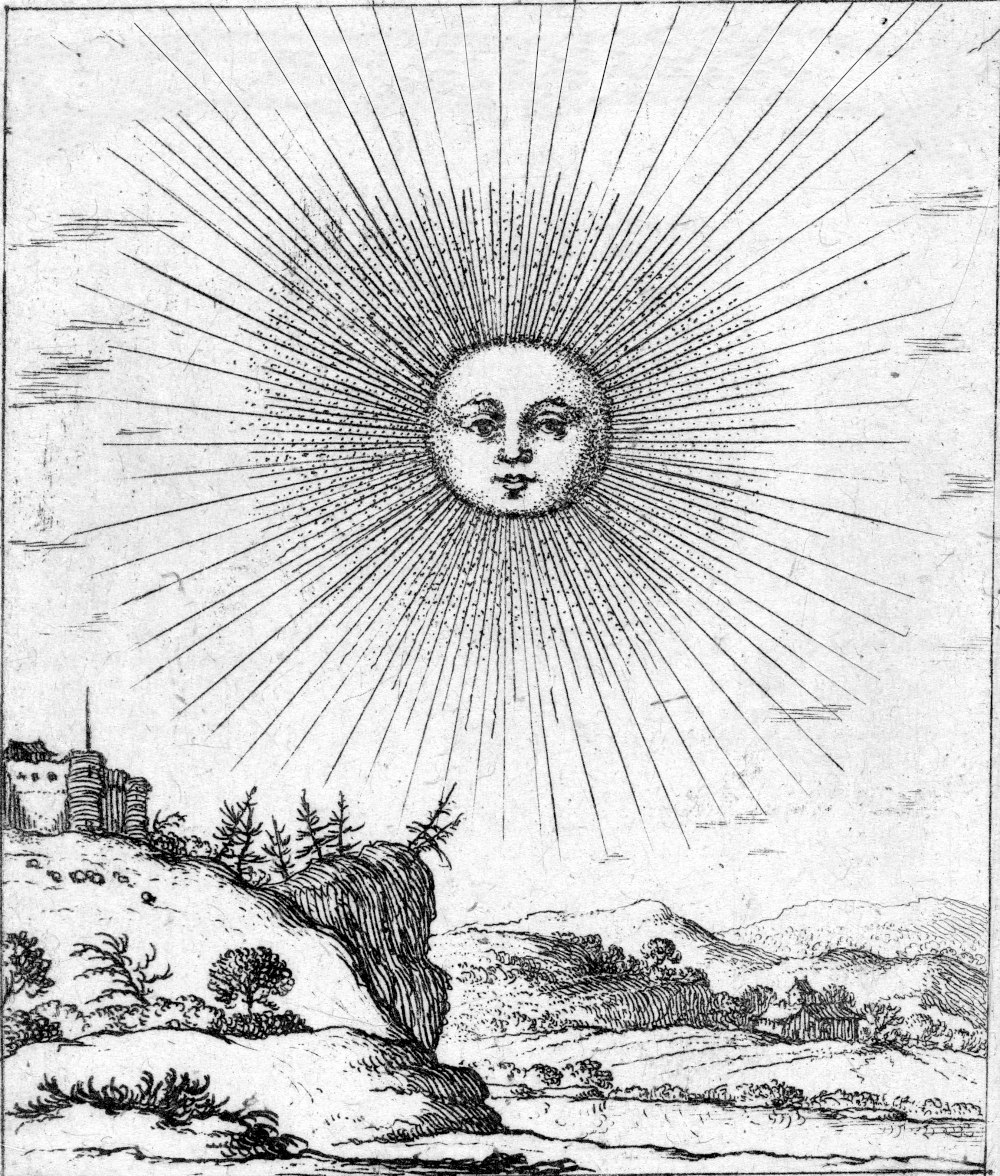
\includegraphics[keepaspectratio,width=0.4\textwidth]{figures/Bright-sun-Albert-Flamen-small.jpg}
  \captionart{BrightSun}
  \label{fig:brightsun}
\end{figure}

The ordinary sports which are used abroad are hawking, hunting, hilares
venandi labores, \authorfootnote{3226}one calls them, because they recreate body and
mind, \authorfootnote{3227}another, the \authorfootnote{3228}best exercise that is, by which alone
many have been \authorfootnote{3229}freed from all feral diseases. Hegesippus, lib. 1.
cap. 37. relates of Herod, that he was eased of a grievous melancholy
by that means. Plato, 7. de leg. highly magnifies it, dividing it into
three parts, by land, water, air. Xenophon, in Cyropaed. graces it with
a great name, Deorum munus, the gift of the gods, a princely sport,
which they have ever used, saith Langius, epist. 59. lib. 2. as well
for health as pleasure, and do at this day, it being the sole almost
and ordinary sport of our noblemen in Europe, and elsewhere all over
the world. Bohemus, de mor. gent. lib. 3. cap. 12. styles it therefore,
studium nobilium, communiter venantur, quod sibi solis licere
contendunt, 'tis all their study, their exercise, ordinary business,
all their talk: and indeed some dote too much after it, they can do
nothing else, discourse of naught else. Paulus Jovius, descr. Brit.
doth in some sort tax our \authorfootnote{3230} English nobility for it, for living in
the country so much, and too frequent use of it, as if they had no
other means but hawking and hunting to approve themselves gentlemen
with.

Hawking comes near to hunting, the one in the air, as the other on the
earth, a sport as much affected as the other, by some preferred.
\authorfootnote{3231}It was never heard of amongst the Romans, invented some twelve
hundred years since, and first mentioned by Firmicus, lib. 5. cap. 8.

The Greek emperors began it, and now nothing so frequent: he is nobody
that in the season hath not a hawk on his fist. A great art, and many
\authorfootnote{3232}books written of it. It is a wonder to hear \authorfootnote{3233}what is related
of the Turks' officers in this behalf, how many thousand men are
employed about it, how many hawks of all sorts, how much revenues
consumed on that only disport, how much time is spent at Adrianople
alone every year to that purpose. The \authorfootnote{3234}Persian kings hawk after
butterflies with sparrows made to that use, and stares: lesser hawks
for lesser games they have, and bigger for the rest, that they may
produce their sport to all seasons. The Muscovian emperors reclaim
eagles to fly at hinds, foxes, \etc{}, and such a one was sent for a
present to \authorfootnote{3235}Queen Elizabeth: some reclaim ravens, castrils, pies,
\etc{}, and man them for their pleasures.

Fowling is more troublesome, but all out as delightsome to some sorts
of men, be it with guns, lime, nets, glades, gins, strings, baits,
pitfalls, pipes, calls, stalking-horses, setting-dogs, decoy-ducks,
\etc{}, or otherwise. Some much delight to take larks with day-nets, small
birds with chaff-nets, plovers, partridge, herons, snipe, \etc{}. Henry the
Third, king of Castile (as Mariana the Jesuit reports of him, lib. 3.
cap. 7.) was much affected \authorfootnote{3236}with catching of quails, and many
gentlemen take a singular pleasure at morning and evening to go abroad
with their quail-pipes, and will take any pains to satisfy their
delight in that kind. The \authorfootnote{3237}Italians have gardens fitted to such
use, with nets, bushes, glades, sparing no cost or industry, and are
very much affected with the sport. Tycho Brahe, that great astronomer,
in the chorography of his Isle of Huena, and Castle of Uraniburge, puts
down his nets, and manner of catching small birds, as an ornament and a
recreation, wherein he himself was sometimes employed.

Fishing is a kind of hunting by water, be it with nets, weels, baits,
angling, or otherwise, and yields all out as much pleasure to some men
as dogs or hawks; \authorfootnote{3238}When they draw their fish upon the bank, saith
Nic. Henselius Silesiographi\ae{}, cap. 3. speaking of that extraordinary
delight his countrymen took in fishing, and in making of pools. James
Dubravius, that Moravian, in his book de pisc. telleth, how travelling
by the highway side in Silesia, he found a nobleman, \authorfootnote{3239}booted up to
the groins, wading himself, pulling the nets, and labouring as much as
any fisherman of them all: and when some belike objected to him the
baseness of his office, he excused himself, \authorfootnote{3240}that if other men
might hunt hares, why should not he hunt carps? Many gentlemen in like
sort with us will wade up to the arm-holes upon such occasions, and
voluntarily undertake that to satisfy their pleasures, which a poor man
for a good stipend would scarce be hired to undergo. Plutarch, in his
book de soler. animal. speaks against all fishing, \authorfootnote{3241}as a filthy,
base, illiberal employment, having neither wit nor perspicacity in it,
nor worth the labour. But he that shall consider the variety of baits
for all seasons, and pretty devices which our anglers have invented,
peculiar lines, false flies, several sleights, \etc{} will say, that it
deserves like commendation, requires as much study and perspicacity as
the rest, and is to be preferred before many of them. Because hawking
and hunting are very laborious, much riding, and many dangers accompany
them; but this is still and quiet: and if so be the angler catch no
fish, yet he hath a wholesome walk to the brookside, pleasant shade by
the sweet silver streams; he hath good air, and sweet smells of fine
fresh meadow flowers, he hears the melodious harmony of birds, he sees
the swans, herons, ducks, water-horns, coots, \etc{}, and many other fowl,
with their brood, which he thinketh better than the noise of hounds, or
blast of horns, and all the sport that they can make.

Many other sports and recreations there be, much in use, as ringing,
bowling, shooting, which Ascam recommends in a just volume, and hath in
former times been enjoined by statute, as a defensive exercise, and an
\authorfootnote{3242}honour to our land, as well may witness our victories in France.

Keelpins, tronks, quoits, pitching bars, hurling, wrestling, leaping,
running, fencing, mustering, swimming, wasters, foils, football,
balloon, quintain, \etc{}, and many such, which are the common recreations
of the country folks. Riding of great horses, running at rings, tilts
and tournaments, horse races, wild-goose chases, which are the disports
of greater men, and good in themselves, though many gentlemen by that
means gallop quite out of their fortunes.

But the most pleasant of all outward pastimes is that of \authorfootnote{3243}Areteus,
\latininlinetrans{strolling through pleasant scenery}{deambulatio per am\oe{}na loca}, to make a petty progress, a merry journey
now and then with some good companions, to visit friends, see cities,
castles, towns,

\textlatin{
\begin{verse}
Visere saepe amnes nitidos, per amaenaque Tempe,\\
Et placidas summis sectari in montibus auras.\authorfootnote{3244}
\end{verse}}

\begin{verse}
To see the pleasant fields, the crystal fountains,\\
And take the gentle air amongst the mountains.
\end{verse}

\authorfootnote{3245}To walk amongst orchards, gardens, bowers, mounts, and arbours,
artificial wildernesses, green thickets, arches, groves, lawns,
rivulets, fountains, and such like pleasant places, like that
Antiochian Daphne, brooks, pools, fishponds, between wood and water, in
a fair meadow, by a river side, \authorfootnote{3246}ubi variae, avium cantationes,
florum colores, pratorum frutices, \etc{} to disport in some pleasant
plain, park, run up a steep hill sometimes, or sit in a shady seat,
must needs be a delectable recreation. Hortus principis et domus ad
delectationem facia, cum sylva, monte et piscina, vulgo la montagna:
the prince's garden at Ferrara \authorfootnote{3247}Schottus highly magnifies, with
the groves, mountains, ponds, for a delectable prospect, he was much
affected with it: a Persian paradise, or pleasant park, could not be
more delectable in his sight. St. Bernard, in the description of his
monastery, is almost ravished with the pleasures of it. A sick
\authorfootnote{3248}man (saith he) sits upon a green bank, and when the dog-star
parcheth the plains, and dries up rivers, he lies in a shady bower,
Fronde sub arborea ferventia temperat astra, and feeds his eyes with
variety of objects, herbs, trees, to comfort his misery, he receives
many delightsome smells, and fills his ears with that sweet and various
harmony of birds: good God (saith he), what a company of pleasures hast
thou made for man! He that should be admitted on a sudden to the sight
of such a palace as that of Escurial in Spain, or to that which the
Moors built at Granada, Fontainebleau in France, the Turk's gardens in
his seraglio, wherein all manner of birds and beasts are kept for
pleasure; wolves, bears, lynxes, tigers, lions, elephants, \etc{}, or upon
the banks of that Thracian Bosphorus: the pope's Belvedere in Rome,
\authorfootnote{3249}as pleasing as those horti pensiles in Babylon, or that Indian
king's delightsome garden in \authorfootnote{3250}\AE{}lian; or \authorfootnote{3251}those famous
gardens of the Lord Cantelow in France, could, not choose, though he
were never so ill paid, but be much recreated for the time; or many of
our noblemen's gardens at home. To take a boat in a pleasant evening,
and with music \authorfootnote{3252}to row upon the waters, which Plutarch so much
applauds, Elian admires, upon the river Pineus: in those Thessalian
fields, beset with green bays, where birds so sweetly sing that
passengers, enchanted as it were with their heavenly music, omnium
laborum et curarum obliviscantur, forget forthwith all labours, care,
and grief: or in a gondola through the Grand Canal in Venice, to see
those goodly palaces, must needs refresh and give content to a
melancholy dull spirit. Or to see the inner rooms of a fair-built and
sumptuous edifice, as that of the Persian kings, so much renowned by
Diodorus and Curtius, in which all was almost beaten gold,
\authorfootnote{3253}chairs, stools, thrones, tabernacles, and pillars of gold, plane
trees, and vines of gold, grapes of precious stones, all the other
ornaments of pure gold,
\authorfootnote{3254}Fulget gemma floris, et jaspide fulva supellex,
Strata micant Tyrio---

With sweet odours and perfumes, generous wines, opiparous fare, \etc{},
besides the gallantest young men, the fairest \authorfootnote{3255}virgins, puellae
scitulae ministrantes, the rarest beauties the world could afford, and
those set out with costly and curious attires, ad stuporem usque
spectantium, with exquisite music, as in \authorfootnote{3256}Trimaltion's house, in
every chamber sweet voices ever sounding day and night, incomparabilis
luxus, all delights and pleasures in each kind which to please the
senses could possibly be devised or had, convives coronati, delitiis
ebrii, \etc{}. Telemachus, in Homer, is brought in as one ravished almost
at the sight of that magnificent palace, and rich furniture of
Menelaus, when he beheld
\authorfootnote{3257}Aeris fulgorem et resonantia tecta corusco
Auro, atque electro nitido, sectoque elephanto,
Argentoque simul. Talis Jovis ardua sedes,
Aulaque coelicolum stellans splendescit Olympo.

Such glittering of gold and brightest brass to shine,
Clear amber, silver pure, and ivory so fine:
Jupiter's lofty palace, where the gods do dwell,
Was even such a one, and did it not excel.

It will laxare animos, refresh the soul of man to see fair-built
cities, streets, theatres, temples, obelisks, \etc{}. The temple of
Jerusalem was so fairly built of white marble, with so many pyramids
covered with gold; tectumque templi fulvo coruscans auro, nimio suo
fulgore obcaecabat oculos itinerantium, was so glorious, and so
glistened afar off, that the spectators might not well abide the sight
of it. But the inner parts were all so curiously set out with cedar,
gold, jewels, \etc{}, as he said of Cleopatra's palace in
Egypt,-\authorfootnote{3258}Crassumque trabes absconderat aurum, that the beholders
were amazed. What so pleasant as to see some pageant or sight go by, as
at coronations, weddings, and such like solemnities, to see an
ambassador or a prince met, received, entertained with masks, shows,
fireworks, \etc{}. To see two kings fight in single combat, as Porus and
Alexander; Canute and Edmund Ironside; Scanderbeg and Ferat Bassa the
Turk; when not honour alone but life itself is at stake, as the
\authorfootnote{3259}poet of Hector,
---nec enim pro tergore Tauri,
Pro bove nec certamen erat, quae praemia cursus
Esse solent, sed pro magni viraque animaque-Hectoris.

To behold a battle fought, like that of Crecy, or Agincourt, or
Poitiers, qua nescio (saith Froissart) an vetustas ullam proferre
possit clariorem. To see one of Caesar's triumphs in old Rome revived,
or the like. To be present at an interview, \authorfootnote{3260}as that famous of
Henry the Eighth and Francis the First, so much renowned all over
Europe; ubi tanto apparatu (saith Hubertus Veillius) tamque triumphali
pompa ambo reges com eorum conjugibus coiere, ut nulla unquam aetas tam
celebria festa viderit aut audieriti, no age ever saw the like. So
infinitely pleasant are such shows, to the sight of which oftentimes
they will come hundreds of miles, give any money for a place, and
remember many years after with singular delight. Bodine, when he was
ambassador in England, said he saw the noblemen go in their robes to
the parliament house, summa cum jucunditate vidimus, he was much
affected with the sight of it. Pomponius Columna, saith Jovius in his
life, saw thirteen Frenchmen, and so many Italians, once fight for a
whole army: Quod jucundissimum spectaculum in vita dicit sua, the
pleasantest sight that ever he saw in his life. Who would not have been
affected with such a spectacle? Or that single combat of \authorfootnote{3261} Breaute
the Frenchman, and Anthony Schets a Dutchman, before the walls of
Sylvaducis in Brabant, anno 1600. They were twenty-two horse on the one
side, as many on the other, which like Livy's Horatii, Torquati and
Corvini fought for their own glory and country's honour, in the sight
and view of their whole city and army. \authorfootnote{3262}When Julius Caesar warred
about the banks of Rhone, there came a barbarian prince to see him and
the Roman army, and when he had beheld Caesar a good while, \authorfootnote{3263}I see
the gods now (saith he) which before I heard of, nec feliciorem ullam
vitae meae aut optavi, aut sensi diem: it was the happiest day that
ever he had in his life. Such a sight alone were able of itself to
drive away melancholy; if not for ever, yet it must needs expel it for
a time. Radzivilus was much taken with the pasha's palace in Cairo, and
amongst many other objects which that place afforded, with that
solemnity of cutting the banks of the Nile by Imbram Pasha, when it
overflowed, besides two or three hundred gilded galleys on the water,
he saw two millions of men gathered together on the land, with turbans
as white as snow; and 'twas a goodly sight. The very reading of feasts,
triumphs, interviews, nuptials, tilts, tournaments, combats, and
monomachies, is most acceptable and pleasant. \authorfootnote{3264} Franciscus Modius
hath made a large collection of such solemnities in two great tomes,
which whoso will may peruse. The inspection alone of those curious
iconographies of temples and palaces, as that of the Lateran church in
Albertus Durer, that of the temple of Jerusalem in \authorfootnote{3265}Josephus,
Adricomius, and Villalpandus: that of the Escurial in Guadas, of Diana
at Ephesus in Pliny, Nero's golden palace in Rome, \authorfootnote{3266}Justinian's in
Constantinople, that Peruvian Jugo's in \authorfootnote{3267}Cusco, ut non ab
hominibus, sed a daemoniis constructum videatur; St. Mark's in Venice,
by Ignatius, with many such; priscorum artificum opera (saith that
\authorfootnote{3268}interpreter of Pausanias), the rare workmanship of those ancient
Greeks, in theatres, obelisks, temples, statues, gold, silver, ivory,
marble images, non minore ferme quum leguntur, quam quum cernuntur,
animum delectatione complent, affect one as much by reading almost as
by sight.

The country hath his recreations, the city his several gymnics and
exercises, May games, feasts, wakes, and merry meetings, to solace
themselves; the very being in the country; that life itself is a
sufficient recreation to some men, to enjoy such pleasures, as those
old patriarchs did. Diocletian, the emperor, was so much affected with
it, that he gave over his sceptre, and turned gardener. Constantine
wrote twenty books of husbandry. Lysander, when ambassadors came to see
him, bragged of nothing more than of his orchard, hi sunt ordines mei.

What shall I say of Cincinnatus, Cato, Tully, and many such? how they
have been pleased with it, to prune, plant, inoculate and graft, to
show so many several kinds of pears, apples, plums, peaches, \etc{}.
\authorfootnote{3269}Nunc captare feras laqueo, nunc fallere visco,
Atque etiam magnos canibus circundare saltus
Insidias avibus moliri, incendere vepres.

Sometimes with traps deceive, with line and string
To catch wild birds and beasts, encompassing
The grove with dogs, and out of bushes firing.

---et nidos aviumscrutari, \etc{}.

Jucundus, in his preface to Cato, Varro, Columella, \etc{}, put out by
him, confesseth of himself, that he was mightily delighted with these
husbandry studies, and took extraordinary pleasure in them: if the
theory or speculation can so much affect, what shall the place and
exercise itself, the practical part do? The same confession I find in
Herbastein, Porta, Camerarius, and many others, which have written of
that subject. If my testimony were aught worth, I could say as much of
myself; I am vere Saturnus; no man ever took more delight in springs,
woods, groves, gardens, walks, fishponds, rivers, \etc{}. But
\authorfootnote{3270}Tantalus a labris sitiens fugientia captat
Flumina;

And so do I; Velle licet, potiri non licet.\authorfootnote{3271}
Every palace, every city almost hath its peculiar walks, cloisters,
terraces, groves, theatres, pageants, games, and several recreations;
every country, some professed gymnics to exhilarate their minds, and
exercise their bodies. The \authorfootnote{3272}Greeks had their Olympian, Pythian,
Isthmian, Nemean games, in honour of Neptune, Jupiter, Apollo; Athens
hers: some for honour, garlands, crowns; for \authorfootnote{3273}beauty, dancing,
running, leaping, like our silver games. The \authorfootnote{3274}Romans had their
feasts, as the Athenians, and Lacedaemonians held their public
banquets, in Pritanaeo, Panathenaeis, Thesperiis, Phiditiis, plays,
naumachies, places for sea-fights, \authorfootnote{3275}theatres, amphitheatres able
to contain 70,000 men, wherein they had several delightsome shows to
exhilarate the people; \authorfootnote{3276} gladiators, combats of men with
themselves, with wild beasts, and wild beasts one with another, like
our bull-baitings, or bear-baitings (in which many countrymen and
citizens amongst us so much delight and so frequently use), dancers on
ropes. Jugglers, wrestlers, comedies, tragedies, publicly exhibited at
the emperor's and city's charge, and that with incredible cost and
magnificence. In the Low-Countries (as \authorfootnote{3277}Meteran relates) before
these wars, they had many solemn feasts, plays, challenges, artillery
gardens, colleges of rhymers, rhetoricians, poets: and to this day,
such places are curiously maintained in Amsterdam, as appears by that
description of Isaacus Pontanus, rerum Amstelrod. lib. 2. cap. 25. So
likewise not long since at Friburg in Germany, as is evident by that
relation of \authorfootnote{3278}Neander, they had Ludos septennales, solemn plays
every seven years, which Bocerus, one of their own poets, hath
elegantly described:
\authorfootnote{3279}At nunc magnifico spectacula structa paratu
Quid memorem, veteri non concessura Quirino,
Ludorum pompa, \etc{}.

In Italy they have solemn declamations of certain select young
gentlemen in Florence (like those reciters in old Rome), and public
theatres in most of their cities, for stage-players and others, to
exercise and recreate themselves. All seasons almost, all places, have
their several pastimes; some in summer, some in winter; some abroad,
some within: some of the body, some of the mind: and diverse men have
diverse recreations and exercises. Domitian, the emperor, was much
delighted with catching flies; Augustus to play with nuts amongst
children; \authorfootnote{3280}Alexander Severus was often pleased to play with whelps
and young pigs. \authorfootnote{3281}Adrian was so wholly enamoured with dogs and
horses, that he bestowed monuments and tombs of them, and buried them
in graves. In foul weather, or when they can use no other convenient
sports, by reason of the time, as we do cock-fighting, to avoid
idleness, I think, (though some be more seriously taken with it, spend
much time, cost and charges, and are too solicitous about it)
\authorfootnote{3282}Severus used partridges and quails, as many Frenchmen do still,
and to keep birds in cages, with which he was much pleased, when at any
time he had leisure from public cares and businesses. He had (saith
Lampridius) tame pheasants, ducks, partridges, peacocks, and some
20,000 ring-doves and pigeons. Busbequius, the emperor's orator, when
he lay in Constantinople, and could not stir much abroad, kept for his
recreation, busying himself to see them fed, almost all manner of
strange birds and beasts; this was something, though not to exercise
his body, yet to refresh his mind. Conradus Gesner, at Zurich in
Switzerland, kept so likewise for his pleasure, a great company of wild
beasts; and (as he saith) took great delight to see them eat their
meat. Turkey gentlewomen, that are perpetual prisoners, still mewed up
according to the custom of the place, have little else beside their
household business, or to play with their children to drive away time,
but to dally with their cats, which they have in delitiis, as many of
our ladies and gentlewomen use monkeys and little dogs. The ordinary
recreations which we have in winter, and in most solitary times busy
our minds with, are cards, tables and dice, shovelboard, chess-play,
the philosopher's game, small trunks, shuttlecock, billiards, music,
masks, singing, dancing, Yule-games, frolics, jests, riddles, catches,
purposes, questions and commands, \authorfootnote{3283}merry tales of errant knights,
queens, lovers, lords, ladies, giants, dwarfs, thieves, cheaters,
witches, fairies, goblins, friars, \etc{}, such as the old woman told
Psyche in \authorfootnote{3284}Apuleius, Boccace novels, and the rest, quarum
auditione pueri delectantur, senes narratione, which some delight to
hear, some to tell; all are well pleased with. Amaranthus, the
philosopher, met Hermocles, Diophantus and Philolaus, his companions,
one day busily discoursing about Epicurus and Democritus' tenets, very
solicitous which was most probable and came nearest to truth: to put
them out of that surly controversy, and to refresh their spirits, he
told them a pleasant tale of Stratocles the physician's wedding, and of
all the particulars, the company, the cheer, the music, \etc{}, for he was
new come from it; with which relation they were so much delighted, that
Philolaus wished a blessing to his heart, and many a good
wedding,\authorfootnote{3285} many such merry meetings might he be at, to please
himself with the sight, and others with the narration of it. News are
generally welcome to all our ears, avide audimus, aures enim hominum
novitate laetantur (\authorfootnote{3286}as Pliny observes), we long after rumour to
hear and listen to it, \authorfootnote{3287}densum humeris bibit aure vulgus. We are
most part too inquisitive and apt to hearken after news, which Caesar,
in his \authorfootnote{3288}Commentaries, observes of the old Gauls, they would be
inquiring of every carrier and passenger what they had heard or seen,
what news abroad?
---quid toto fiat in orbe,
Quid Seres, quid Thraces agant, secreta novercae,
Et pueri, quis amet, \etc{}.

as at an ordinary with us, bakehouse or barber's shop. When that great
Gonsalva was upon some displeasure confined by King Ferdinand to the
city of Loxa in Andalusia, the only, comfort (saith \authorfootnote{3289}Jovius) he
had to ease his melancholy thoughts, was to hear news, and to listen
after those ordinary occurrences which were brought him cum primis, by
letters or otherwise out of the remotest parts of Europe. Some men's
whole delight is, to take tobacco, and drink all day long in a tavern
or alehouse, to discourse, sing, jest, roar, talk of a cock and bull
over a pot, \etc{}. Or when three or four good companions meet, tell old
stories by the fireside, or in the sun, as old folks usually do, quae
aprici meminere senes, remembering afresh and with pleasure ancient
matters, and such like accidents, which happened in their younger
years: others' best pastime is to game, nothing to them so pleasant.
\authorfootnote{3290}Hic Veneri indulget, hunc decoquit alea-many too nicely take
exceptions at cards, \authorfootnote{3291}tables, and dice, and such mixed lusorious
lots, whom Gataker well confutes. Which though they be honest
recreations in themselves, yet may justly be otherwise excepted at, as
they are often abused, and forbidden as things most pernicious; insanam
rem et damnosam, \authorfootnote{3292}Lemnius calls it. For most part in these kind of
disports 'tis not art or skill, but subtlety, cony-catching, knavery,
chance and fortune carries all away: 'tis ambulatoria pecunia,
\authorfootnote{3293}---puncto mobilis horae
Permutat dominos, et cedit in altera jura.

They labour most part not to pass their time in honest disport, but for
filthy lucre, and covetousness of money. In foedissimum lucrum et
avaritiam hominum convertitur, as Daneus observes. Fons fraudum et
maleficiorum, 'tis the fountain of cozenage and villainy. \authorfootnote{3294}A thing
so common all over Europe at this day, and so generally abused, that
many men are utterly undone by it, their means spent, patrimonies
consumed, they and their posterity beggared; besides swearing,
wrangling, drinking, loss of time, and such inconveniences, which are
ordinary concomitants: \authorfootnote{3295}for when once they have got a haunt of
such companies, and habit of gaming, they can hardly be drawn from it,
but as an itch it will tickle them, and as it is with whoremasters,
once entered, they cannot easily leave it off: Vexat mentes insania
cupido, they are mad upon their sport. And in conclusion (which Charles
the Seventh, that good French king, published in an edict against
gamesters) unde piae et hilaris vitae, suffugium sibi suisque liberis,
totique familiae, \etc{}. That which was once their livelihood, should have
maintained wife, children, family, is now spent and gone; maeror et
egestas, \etc{}, sorrow and beggary succeeds. So good things may be
abused, and that which was first invented to \authorfootnote{3296} refresh men's weary
spirits, when they come from other labours and studies to exhilarate
the mind, to entertain time and company, tedious otherwise in those
long solitary winter nights, and keep them from worse matters, an
honest exercise is contrarily perverted.

Chess-play is a good and witty exercise of the mind for some kind of
men, and fit for such melancholy, Rhasis holds, as are idle, and have
extravagant impertinent thoughts, or troubled with cares, nothing
better to distract their mind, and alter their meditations: invented
(some say) by the \authorfootnote{3297}general of an army in a famine, to keep
soldiers from mutiny: but if it proceed from overmuch study, in such a
case it may do more harm than good; it is a game too troublesome for
some men's brains, too full of anxiety, all out as bad as study;
besides it is a testy choleric game, and very offensive to him that
loseth the mate. \authorfootnote{3298}William the Conqueror, in his younger years,
playing at chess with the Prince of France (Dauphine was not annexed to
that crown in those days) losing a mate, knocked the chess-board about
his pate, which was a cause afterward of much enmity between them. For
some such reason it is belike, that Patritius, in his 3. book, tit. 12.
de reg. instit. forbids his prince to play at chess; hawking and
hunting, riding, \etc{} he will allow; and this to other men, but by no
means to him. In Muscovy, where they live in stoves and hot houses all
winter long, come seldom or little abroad, it is again very necessary,
and therefore in those parts, (saith \authorfootnote{3299}Herbastein) much used. At
Fez in Africa, where the like inconvenience of keeping within doors is
through heat, it is very laudable; and (as \authorfootnote{3300}Leo Afer relates) as
much frequented. A sport fit for idle gentlewomen, soldiers in
garrison, and courtiers that have nought but love matters to busy
themselves about, but not altogether so convenient for such as are
students. The like I may say of Col. Bruxer's philosophy game, D.
Fulke's Metromachia and his Ouronomachia, with the rest of those
intricate astrological and geometrical fictions, for such especially as
are mathematically given; and the rest of those curious games.

Dancing, singing, masking, mumming, stage plays, howsoever they be
heavily censured by some severe Catos, yet if opportunely and soberly
used, may justly be approved. Melius est foedere, quam saltare,
\authorfootnote{3301}saith Austin: but what is that if they delight in it? \authorfootnote{3302}Nemo
saltat sobrius. But in what kind of dance? I know these sports have
many oppugners, whole volumes writ against them; when as all they say
(if duly considered) is but ignoratio Elenchi; and some again, because
they are now cold and wayward, past themselves, cavil at all such
youthful sports in others, as he did in the comedy; they think them,
illico nasci senes, \etc{}. Some out of preposterous zeal object many times
trivial arguments, and because of some abuse, will quite take away the
good use, as if they should forbid wine because it makes men drunk; but
in my judgment they are too stern: there is a time for all things, a
time to mourn, a time to dance, Eccles. \rn{iii.} 4. a time to embrace, a
time not to embrace, (verse 5.) and nothing better than that a man
should rejoice in his own works, verse 22; for my part, I will
subscribe to the king's declaration, and was ever of that mind, those
May games, wakes, and Whitsun ales, \etc{}, if they be not at unseasonable
hours, may justly be permitted. Let them freely feast, sing and dance,
have their puppet-plays, hobby-horses, tabors, crowds, bagpipes, \etc{},
play at ball, and barley-breaks, and what sports and recreations they
like best. In Franconia, a province of Germany, (saith \authorfootnote{3303}Aubanus
Bohemus) the old folks, after evening prayer, went to the alehouse, the
younger sort to dance: and to say truth with \authorfootnote{3304}Salisburiensis,
satius fuerat sic otiari, quam turpius occupari, better to do so than
worse, as without question otherwise (such is the corruption of man's
nature) many of them will do. For that cause, plays, masks, jesters,
gladiators, tumblers, jugglers, \etc{}, and all that crew is admitted and
winked at: \authorfootnote{3305}Tota jocularium scena procedit, et ideo spectacula
admissa sunt, et infinita tyrocinia vanitatum, ut his occupentur, qui
perniciosius otiari solent: that they might be busied about such toys,
that would otherwise more perniciously be idle. So that as
\authorfootnote{3306}Tacitus said of the astrologers in Rome, we may say of them,
genus hominum est quod in civitate nostra et vitabitur semper et
retinebitur, they are a debauched company most part, still spoken
against, as well they deserve some of them (for I so relish and
distinguish them as fiddlers, and musicians), and yet ever retained.

Evil is not to be done (I confess) that good may come of it: but this
is evil per accidens, and in a qualified sense, to avoid a greater
inconvenience, may justly be tolerated. Sir Thomas More, in his Utopian
Commonwealth, \authorfootnote{3307}as he will have none idle, so will he have no man
labour over hard, to be toiled out like a horse, 'tis more than slavish
infelicity, the life of most of our hired servants and tradesmen
elsewhere (excepting his Utopians) but half the day allotted for work,
and half for honest recreation, or whatsoever employment they shall
think fit for themselves. If one half day in a week were allowed to our
household servants for their merry meetings, by their hard masters, or
in a year some feasts, like those Roman Saturnals, I think they would
labour harder all the rest of their time, and both parties be better
pleased: but this needs not (you will say), for some of them do nought
but loiter all the week long.

This which I aim at, is for such as are fracti animis, troubled in
mind, to ease them, over-toiled on the one part, to refresh: over idle
on the other, to keep themselves busied. And to this purpose, as any
labour or employment will serve to the one, any honest recreation will
conduce to the other, so that it be moderate and sparing, as the use of
meat and drink; not to spend all their life in gaming, playing, and
pastimes, as too many gentlemen do; but to revive our bodies and
recreate our souls with honest sports: of which as there be diverse
sorts, and peculiar to several callings, ages, sexes, conditions, so
there be proper for several seasons, and those of distinct natures, to
fit that variety of humours which is amongst them, that if one will
not, another may: some in summer, some in winter, some gentle, some
more violent, some for the mind alone, some for the body and mind: (as
to some it is both business and a pleasant recreation to oversee
workmen of all sorts, husbandry, cattle, horses, \etc{}. To build, plot,
project, to make models, cast up accounts, \etc{}) some without, some
within doors; new, old, \etc{}, as the season serveth, and as men are
inclined. It is reported of Philippus Bonus, that good duke of Burgundy
(by Lodovicus Vives, in Epist. and Pont. \authorfootnote{3308}Heuter in his history)
that the said duke, at the marriage of Eleonora, sister to the king of
Portugal, at Bruges in Flanders, which was solemnised in the deep of
winter, when, as by reason of unseasonable weather, he could neither
hawk nor hunt, and was now tired with cards, dice, \etc{}, and such other
domestic sports, or to see ladies dance, with some of his courtiers, he
would in the evening walk disguised all about the town. It so fortuned,
as he was walking late one night, he found a country fellow dead drunk,
snorting on a bulk; \authorfootnote{3309}he caused his followers to bring him to his
palace, and there stripping him of his old clothes, and attiring him
after the court fashion, when he waked, he and they were all ready to
attend upon his excellency, persuading him he was some great duke. The
poor fellow admiring how he came there, was served in state all the day
long; after supper he saw them dance, heard music, and the rest of
those court-like pleasures: but late at night, when he was well
tippled, and again fast asleep, they put on his old robes, and so
conveyed him to the place where they first found him. Now the fellow
had not made them so good sport the day before as he did when he
returned to himself; all the jest was, to see how he \authorfootnote{3310}looked upon
it. In conclusion, after some little admiration, the poor man told his
friends he had seen a vision, constantly believed it, would not
otherwise be persuaded, and so the jest ended. \authorfootnote{3311}Antiochus
Epiphanes would often disguise himself, steal from his court, and go
into merchants', goldsmiths', and other tradesmen's shops, sit and talk
with them, and sometimes ride or walk alone, and fall aboard with any
tinker, clown, serving man, carrier, or whomsoever he met first.

Sometimes he did ex insperato give a poor fellow money, to see how he
would look, or on set purpose lose his purse as he went, to watch who
found it, and withal how he would be affected, and with such objects he
was much delighted. Many such tricks are ordinarily put in practice by
great men, to exhilarate themselves and others, all which are harmless
jests, and have their good uses.

But amongst those exercises, or recreations of the mind within doors,
there is none so general, so aptly to be applied to all sorts of men,
so fit and proper to expel idleness and melancholy, as that of study:
Studia, senectutem oblectant, adolescentiam, alunt, secundas res
ornant, adversis perfugium et solatium praebent, domi delectant, \etc{},
find the rest in Tully pro Archia Poeta. \authorfootnote{3312}What so full of content,
as to read, walk, and see maps, pictures, statues, jewels, marbles,
which some so much magnify, as those that Phidias made of old so
exquisite and pleasing to be beheld, that as \authorfootnote{3313}Chrysostom thinketh,
if any man be sickly, troubled in mind, or that cannot sleep for grief,
and shall but stand over against one of Phidias' images, he will forget
all care, or whatsoever else may molest him, in an instant? There be
those as much taken with Michael Angelo's, Raphael de Urbino's,
Francesco Francia's pieces, and many of those Italian and Dutch
painters, which were excellent in their ages; and esteem of it as a
most pleasing sight, to view those neat architectures, devices,
escutcheons, coats of arms, read such books, to peruse old coins of
several sorts in a fair gallery; artificial works, perspective glasses,
old relics, Roman antiquities, variety of colours. A good picture is
falsa veritas, et muta poesis: and though (as \authorfootnote{3314}Vives saith)
artificialia delectant, sed mox fastidimus, artificial toys please but
for a time; yet who is he that will not be moved with them for the
present? When Achilles was tormented and sad for the loss of his dear
friend Patroclus, his mother Thetis brought him a most elaborate and
curious buckler made by Vulcan, in which were engraven sun, moon,
stars, planets, sea, land, men fighting, running, riding, women
scolding, hills, dales, towns, castles, brooks, rivers, trees, \etc{},
with many pretty landscapes, and perspective pieces: with sight of
which he was infinitely delighted, and much eased of his grief.
\authorfootnote{3315}Continuo eo spectaculo captus delenito maerore
Oblectabatur, in manibus tenens dei splendida dona.

Who will not be affected so in like case, or see those well-furnished
cloisters and galleries of the Roman cardinals, so richly stored with
all modern pictures, old statues and antiquities? Cum se-spectando
recreet simul et legendo, to see their pictures alone and read the
description, as \authorfootnote{3316}Boisardus well adds, whom will it not affect?
which Bozius, Pomponius, Laetus, Marlianus, Schottus, Cavelerius,
Ligorius, \etc{}, and he himself hath well performed of late. Or in some
prince's cabinets, like that of the great dukes in Florence, of Felix
Platerus in Basil, or noblemen's houses, to see such variety of
attires, faces, so many, so rare, and such exquisite pieces, of men,
birds, beasts, \etc{}, to see those excellent landscapes, Dutch works, and
curious cuts of Sadlier of Prague, Albertus Durer, Goltzius Vrintes,
\etc{}, such pleasant pieces of perspective, Indian pictures made of
feathers, China works, frames, thaumaturgical motions, exotic toys, \etc{}.

Who is he that is now wholly overcome with idleness, or otherwise
involved in a labyrinth of worldly cares, troubles and discontents,
that will not be much lightened in his mind by reading of some enticing
story, true or feigned, whereas in a glass he shall observe what our
forefathers have done, the beginnings, ruins, falls, periods of
commonwealths, private men's actions displayed to the life, \etc{}. \authorfootnote{3317}
Plutarch therefore calls them, secundas mensas et bellaria, the second
course and junkets, because they were usually read at noblemen's
feasts. Who is not earnestly affected with a passionate speech, well
penned, an elegant poem, or some pleasant bewitching discourse, like
that of \authorfootnote{3318} Heliodorus, ubi oblectatio quaedam placide fuit, cum
hilaritate conjuncta? Julian the Apostate was so taken with an oration
of Libanius, the sophister, that, as he confesseth, he could not be
quiet till he had read it all out. Legi orationem tuam magna ex parte,
hesterna die ante prandium, pransus vero sine ulla intermissione totam
absolvi.\authorfootnote{3319}O argumenta! O compositionem! I may say the same of this
or that pleasing tract, which will draw his attention along with it. To
most kind of men it is an extraordinary delight to study. For what a
world of books offers itself, in all subjects, arts, and sciences, to
the sweet content and capacity of the reader? In arithmetic, geometry,
perspective, optics, astronomy, architecture, sculpture, painting, of
which so many and such elaborate treatises are of late written: in
mechanics and their mysteries, military matters, navigation,
\authorfootnote{3320}riding of horses, \authorfootnote{3321}fencing, swimming, gardening, planting,
great tomes of husbandry, cookery, falconry, hunting, fishing, fowling,
\etc{}, with exquisite pictures of all sports, games, and what not? In
music, metaphysics, natural and moral philosophy, philology, in policy,
heraldry, genealogy, chronology, \etc{}, they afford great tomes, or those
studies of \authorfootnote{3322}antiquity, \etc{}, et \authorfootnote{3323}quid subtilius Arithmeticis
inventionibus, quid jucundius Musicis rationibus, quid divinius
Astronomicis, quid rectius Geometricis demonstrationibus? What so sure,
what so pleasant? He that shall but see that geometrical tower of
Garezenda at Bologna in Italy, the steeple and clock at Strasburg, will
admire the effects of art, or that engine of Archimedes, to remove the
earth itself, if he had but a place to fasten his instrument:
Archimedes Coclea, and rare devices to corrivate waters, musical
instruments, and tri-syllable echoes again, again, and again repeated,
with myriads of such. What vast tomes are extant in law, physic, and
divinity, for profit, pleasure, practice, speculation, in verse or
prose, \etc{}! their names alone are the subject of whole volumes, we have
thousands of authors of all sorts, many great libraries full well
furnished, like so many dishes of meat, served out for several palates;
and he is a very block that is affected with none of them. Some take an
infinite delight to study the very languages wherein these books are
written, Hebrew, Greek, Syriac, Chaldee, Arabic, \etc{}. Methinks it would
please any man to look upon a geographical map, \authorfootnote{3324}sauvi animum
delectatione allicere, ob incredibilem rerum varietatem et
jucunditatem, et ad pleniorem sui cognitionem excitare, chorographical,
topographical delineations, to behold, as it were, all the remote
provinces, towns, cities of the world, and never to go forth of the
limits of his study, to measure by the seale and compass their extent,
distance, examine their site. Charles the Great, as Platina writes, had
three fair silver tables, in one of which superficies was a large map
of Constantinople, in the second Rome neatly engraved, in the third an
exquisite description of the whole world, and much delight he took in
them. What greater pleasure can there now be, than to view those
elaborate maps of Ortelius, \authorfootnote{3325}Mercator, Hondius, \etc{}? To peruse
those books of cities, put out by Braunus and Hogenbergius? To read
those exquisite descriptions of Maginus, Munster, Herrera, Laet,
Merula, Boterus, Leander, Albertus, Camden, Leo Afer, Adricomius, Nic.
Gerbelius, \etc{}? Those famous expeditions of Christoph. Columbus,
Americus Vespucius, Marcus Polus the Venetian, Lod. Vertomannus,
Aloysius Cadamustus, \etc{}? Those accurate diaries of Portuguese,
Hollanders, of Bartison, Oliver a Nort, \etc{}. Hakluyt's voyages, Pet.
Martyr's Decades, Benzo, Lerius, Linschoten's relations, those
Hodoeporicons of Jod. a Meggen, Brocard the monk, Bredenbachius, Jo.
Dublinius, Sands, \etc{}, to Jerusalem, Egypt, and other remote places of
the world? those pleasant itineraries of Paulus Hentzerus, Jodocus
Sincerus, Dux Polonus, \etc{}, to read Bellonius' observations, P. Gillius
his surveys; those parts of America, set out, and curiously cut in
pictures, by Fratres a Bry. To see a well-cut herbal, herbs, trees,
flowers, plants, all vegetables expressed in their proper colours to
the life, as that of Matthiolus upon Dioscorides, Delacampius, Lobel,
Bauhinus, and that last voluminous and mighty herbal of Beslar of
Nuremberg, wherein almost every plant is to his own bigness. To see
birds, beasts, and fishes of the sea, spiders, gnats, serpents, flies,
\etc{}, all creatures set out by the same art, and truly expressed in
lively colours, with an exact description of their natures, virtues,
qualities, \etc{}, as hath been accurately performed by \AE{}lian, Gesner,
Ulysses Aldrovandus, Bellonius, Rondoletius, Hippolitus Salvianus, \etc{}.
\authorfootnote{3326}Arcana coeli, naturae secreta, ordinem universi scire majoris
felicitatis et dulcedinis est, quam cogitatione quis assequi possit,
aut mortalis sperare. What more pleasing studies can there be than the
mathematics, theoretical or practical parts? as to survey land, make
maps, models, dials, \etc{}, with which I was ever much delighted myself.

Tails est Mathematum pulchritudo (saith \authorfootnote{3327} Plutarch) ut his
indignum sit divitiarum phaleras istas et bullas, et puellaria
spectacula comparari; such is the excellency of these studies, that all
those ornaments and childish bubbles of wealth, are not worthy to be
compared to them: credi mihi ( \authorfootnote{3328}saith one) extingui dulce erit
Mathematicarum artium studio, I could even live and die with such
meditation, \authorfootnote{3329}and take more delight, true content of mind in them,
than thou hast in all thy wealth and sport, how rich soever thou art.

And as \authorfootnote{3330}Cardan well seconds me, Honorificum magis est et gloriosum
haec intelligere, quam provinciis praeesse, formosum aut ditem juvenem
esse. \authorfootnote{3331}The like pleasure there is in all other studies, to such as
are truly addicted to them, \authorfootnote{3332}ea suavitas (one holds) ut cum quis
ea degustaverit, quasi poculis Circeis captus, non possit unquam ab
illis divelli; the like sweetness, which as Circe's cup bewitcheth a
student, he cannot leave off, as well may witness those many laborious
hours, days and nights, spent in the voluminous treatises written by
them; the same content. \authorfootnote{3333}Julius Scaliger was so much affected with
poetry, that he brake out into a pathetical protestation, he had rather
be the author of twelve verses in Lucan, or such an ode in
\authorfootnote{3334}Horace, than emperor of Germany. \authorfootnote{3335}Nicholas Gerbelius, that
good old man, was so much ravished with a few Greek authors restored to
light, with hope and desire of enjoying the rest, that he exclaims
forthwith, Arabibus atque Indis omnibus erimus ditiores, we shall be
richer than all the Arabic or Indian princes; of such \authorfootnote{3336}esteem they
were with him, incomparable worth and value. Seneca prefers Zeno and
Chrysippus, two doting stoics (he was so much enamoured of their
works), before any prince or general of an army; and Orontius, the
mathematician, so far admires Archimedes, that he calls him Divinum et
homine majorem, a petty god, more than a man; and well he might, for
aught I see, if you respect fame or worth. Pindarus, of Thebes, is as
much renowned for his poems, as Epaminondas, Pelopidas, Hercules or
Bacchus, his fellow citizens, for their warlike actions; et si famam
respicias, non pauciores Aristotelis quam Alexandri meminerunt (as
Cardan notes), Aristotle is more known than Alexander; for we have a
bare relation of Alexander's deeds, but Aristotle, totus vivit in
monumentis, is whole in his works: yet I stand not upon this; the
delight is it, which I aim at, so great pleasure, such sweet content
there is in study. \authorfootnote{3337}King James, 1605, when he came to see our
University of Oxford, and amongst other edifices now went to view that
famous library, renewed by Sir Thomas Bodley, in imitation of
Alexander, at his departure brake out into that noble speech, If I were
not a king, I would be a university man: \authorfootnote{3338} and if it were so that
I must be a prisoner, if I might have my wish, I would desire to have
no other prison than that library, and to be chained together with so
many good authors et mortuis magistris. So sweet is the delight of
study, the more learning they have (as he that hath a dropsy, the more
he drinks the thirstier he is) the more they covet to learn, and the
last day is prioris discipulus; harsh at first learning is, radices
amarcae, but fractus dulces, according to that of Isocrates, pleasant
at last; the longer they live, the more they are enamoured with the
Muses. Heinsius, the keeper of the library at Leyden in Holland, was
mewed up in it all the year long: and that which to thy thinking should
have bred a loathing, caused in him a greater liking. \authorfootnote{3339}I no sooner
(saith he) come into the library, but I bolt the door to me, excluding
lust, ambition, avarice, and all such vices, whose nurse is idleness,
the mother of ignorance, and melancholy herself, and in the very lap of
eternity, amongst so many divine souls, I take my seat, with so lofty a
spirit and sweet content, that I pity all our great ones, and rich men
that know not this happiness. I am not ignorant in the meantime
(notwithstanding this which I have said) how barbarously and basely,
for the most part, our ruder gentry esteem of libraries and books, how
they neglect and contemn so great a treasure, so inestimable a benefit,
as Aesop's cock did the jewel he found in the dunghill; and all through
error, ignorance, and want of education. And 'tis a wonder, withal, to
observe how much they will vainly cast away in unnecessary expenses,
quot modis pereant (saith \authorfootnote{3340}Erasmus) magnatibus pecuniae, quantum
absumant alea, scorta, compotationes, profectiones non necessariae,
pompae, bella quaesita, ambitio, colax, morio, ludio, \etc{}, what in
hawks, hounds, lawsuits, vain building, gormandising, drinking, sports,
plays, pastimes, \etc{}. If a well-minded man to the Muses, would sue to
some of them for an exhibition, to the farther maintenance or
enlargement of such a work, be it college, lecture, library, or
whatsoever else may tend to the advancement of learning, they are so
unwilling, so averse, that they had rather see these which are already,
with such cost and care erected, utterly ruined, demolished or
otherwise employed; for they repine many and grudge at such gifts and
revenues so bestowed: and therefore it were in vain, as Erasmus well
notes, vel ab his, vel a negotiatoribus qui se Mammonae dediderunt,
improbum fortasse tale officium exigere, to solicit or ask anything of
such men that are likely damned to riches; to this purpose. For my part
I pity these men, stultos jubeo esse libenter, let them go as they are,
in the catalogue of Ignoramus. How much, on the other side, are all we
bound that are scholars, to those munificent Ptolemies, bountiful
Maecenases, heroical patrons, divine spirits,
\authorfootnote{3341}---qui nobis haec otio fecerunt, namque erit ille mihi semper
Deus---

These blessings, friend, a Deity bestow'd,
For never can I deem him less than God.

that have provided for us so many well-furnished libraries, as well in
our public academies in most cities, as in our private colleges? How
shall I remember \authorfootnote{3342}Sir Thomas Bodley, amongst the rest, \authorfootnote{3343}Otho
Nicholson, and the Right Reverend John Williams, Lord Bishop of Lincoln
(with many other pious acts), who besides that at St. John's College in
Cambridge, that in Westminster, is now likewise in Fieri with a library
at Lincoln (a noble precedent for all corporate towns and cities to
imitate), O quam te memorem (vir illustrissime) quibus elogiis? But to
my task again.

Whosoever he is therefore that is overrun with solitariness, or carried
away with pleasing melancholy and vain conceits, and for want of
employment knows not how to spend his time, or crucified with worldly
care, I can prescribe him no better remedy than this of study, to
compose himself to the learning of some art or science. Provided always
that this malady proceed not from overmuch study; for in such case he
adds fuel to the fire, and nothing can be more pernicious: let him take
heed he do not overstretch his wits, and make a skeleton of himself; or
such inamoratos as read nothing but play-books, idle poems, jests,
Amadis de Gaul, the Knight of the Sun, the Seven Champions, Palmerin de
Oliva, Huon of Bordeaux, \etc{}. Such many times prove in the end as mad as
Don Quixote. Study is only prescribed to those that are otherwise idle,
troubled in mind, or carried headlong with vain thoughts and
imaginations, to distract their cogitations (although variety of study,
or some serious subject, would do the former no harm) and divert their
continual meditations another way. Nothing in this case better than
study; semper aliquid memoriter ediscant, saith Piso, let them learn
something without book, transcribe, translate, \etc{}. Read the Scriptures,
which Hyperius, lib. 1. de quotid. script. lec. fol. 77. holds
available of itself, \authorfootnote{3344}the mind is erected thereby from all worldly
cares, and hath much quiet and tranquillity. For as \authorfootnote{3345}Austin well
hath it, 'tis scientia scientiarum, omni melle dulcior, omni pane
suavior, omni vino, hilarior: 'tis the best nepenthe, surest cordial,
sweetest alterative, presentest diverter: for neither as
\authorfootnote{3346}Chrysostom well adds, those boughs and leaves of trees which are
plashed for cattle to stand under, in the heat of the day, in summer,
so much refresh them with their acceptable shade, as the reading of the
Scripture doth recreate and comfort a distressed soul, in sorrow and
affliction. Paul bids pray continually; quod cibus corpori, lectio
animae facit, saith Seneca, as meat is to the body, such is reading to
the soul. \authorfootnote{3347}To be at leisure without books is another hell, and to
be buried alive. \authorfootnote{3348}Cardan calls a library the physic of the soul;
\authorfootnote{3349}divine authors fortify the mind, make men bold and constant; and
(as Hyperius adds) godly conference will not permit the mind to be
tortured with absurd cogitations. Rhasis enjoins continual conference
to such melancholy men, perpetual discourse of some history, tale,
poem, news, \etc{}, alternos sermones edere ac bibere, aeque jucundum quam
cibus, sive potus, which feeds the mind as meat and drink doth the
body, and pleaseth as much: and therefore the said Rhasis, not without
good cause, would have somebody still talk seriously, or dispute with
them, and sometimes \authorfootnote{3350}to cavil and wrangle (so that it break not
out to a violent perturbation), for such altercation is like stirring
of a dead fire to make it burn afresh, it whets a dull spirit, and will
not suffer the mind to be drowned in those profound cogitations, which
melancholy men are commonly troubled with. \authorfootnote{3351}Ferdinand and
Alphonsus, kings of Arragon and Sicily, were both cured by reading the
history, one of Curtius, the other of Livy, when no prescribed physic
would take place. \authorfootnote{3352}Camerarius relates as much of Lorenzo de'
Medici. Heathen philosophers arc so full of divine precepts in this
kind, that, as some think, they alone are able to settle a distressed
mind. \authorfootnote{3353}Sunt verba et voces, quibus hunc lenire dolorem, \etc{}.

Epictetus, Plutarch, and Seneca; qualis ille, quae tela, saith Lipsius,
adversus omnes animi casus administrat, et ipsam mortem, quomodo vitia
eripit, infert virtutes? when I read Seneca, \authorfootnote{3354}methinks I am beyond
all human fortunes, on the top of a hill above mortality. Plutarch
saith as much of Homer, for which cause belike Niceratus, in Xenophon,
was made by his parents to con Homer's Iliads and Odysseys without
book, ut in virum bonum evaderet, as well to make him a good and honest
man, as to avoid idleness. If this comfort be got from philosophy, what
shall be had from divinity? What shall Austin, Cyprian, Gregory,
Bernard's divine meditations afford us?

\authorfootnote{3355}Qui quid sit pulchrum, quid turpe, quid utile, quid non,
Plenius et melius Chrysippo et Crantore dicunt.

Nay, what shall the Scripture itself? Which is like an apothecary's
shop, wherein are all remedies for all infirmities of mind, purgatives,
cordials, alteratives, corroboratives, lenitives, \etc{}. Every disease of
the soul, saith \authorfootnote{3356}Austin, hath a peculiar medicine in the
Scripture; this only is required, that the sick man take the potion
which God hath already tempered. \authorfootnote{3357}Gregory calls it a glass wherein
we may see all our infirmities, ignitum colloquium, Psalm \rn{cxix.} 140.
\authorfootnote{3358}Origen a charm. And therefore Hierom prescribes Rusticus the
monk, \authorfootnote{3359}continually to read the Scripture, and to meditate on that
which he hath read; for as mastication is to meat, so is meditation on
that which we read. I would for these causes wish him that, is
melancholy to use both human and divine authors, voluntarily to impose
some task upon himself, to divert his melancholy thoughts: to study the
art of memory, Cosmus Rosselius, Pet. Ravennas, Scenkelius' Detectus,
or practise brachygraphy, \etc{}, that will ask a great deal of attention:
or let him demonstrate a proposition in Euclid, in his five last books,
extract a square root, or study Algebra: than which, as \authorfootnote{3360}Clavius
holds, in all human disciplines nothing can be more excellent and
pleasant, so abstruse and recondite, so bewitching, so miraculous, so
ravishing, so easy withal and full of delight, omnem humanum captum
superare videtur. By this means you may define ex ungue leonem, as the
diverb is, by his thumb alone the bigness of Hercules, or the true
dimensions of the great \authorfootnote{3361}Colossus, Solomon's temple, and
Domitian's amphitheatre out of a little part. By this art you may
contemplate the variation of the twenty-three letters, which may be so
infinitely varied, that the words complicated and deduced thence will
not be contained within the compass of the firmament; ten words may be
varied 40,320 several ways: by this art you may examine how many men
may stand one by another in the whole superficies of the earth, some
say 148,456,800,000,000, assignando singulis passum quadratum
(assigning a square foot to each), how many men, supposing all the
world as habitable as France, as fruitful and so long-lived, may be
born in 60,000 years, and so may you demonstrate with \authorfootnote{3362}Archimedes
how many sands the mass of the whole world might contain if all sandy,
if you did but first know how much a small cube as big as a
mustard-seed might hold, with infinite such. But in all nature what is
there so stupendous as to examine and calculate the motion of the
planets, their magnitudes, apogees, perigees, eccentricities, how far
distant from the earth, the bigness, thickness, compass of the
firmament, each star, with their diameters and circumference, apparent
area, superficies, by those curious helps of glasses, astrolabes,
sextants, quadrants, of which Tycho Brahe in his mechanics, optics
(\authorfootnote{3363}divine optics) arithmetic, geometry, and such like arts and
instruments? What so intricate and pleasing withal, as to peruse and
practise Heron Alexandrinus's works, de spiritalibus, de machinis
bellicis, de machina se movente, Jordani Nemorarii de ponderibus
proposit. 13, that pleasant tract of Machometes Bragdedinus de
superficierum divisionibus, Apollonius's Conics, or Commandinus's
labours in that kind, de centro gravitatis, with many such geometrical
theorems and problems? Those rare instruments and mechanical inventions
of Jac. Bessonus, and Cardan to this purpose, with many such
experiments intimated long since by Roger Bacon, in his tract de
\authorfootnote{3364}Secretis artis et naturae, as to make a chariot to move sine
animali, diving boats, to walk on the water by art, and to fly in the
air, to make several cranes and pulleys, quibus homo trahat ad se mille
homines, lift up and remove great weights, mills to move themselves,
Archita's dove, Albertus's brazen head, and such thaumaturgical works.

But especially to do strange miracles by glasses, of which Proclus and
Bacon writ of old, burning glasses, multiplying glasses, perspectives,
ut unus homo appareat exercitus, to see afar off, to represent solid
bodies by cylinders and concaves, to walk in the air, ut veraciter
videant, (saith Bacon) aurum et argentum et quicquid aliud volunt, et
quum veniant ad locum visionis, nihil inveniant, which glasses are much
perfected of late by Baptista Porta and Galileo, and much more is
promised by Maginus and Midorgius, to be performed in this kind.

Otocousticons some speak of, to intend hearing, as the other do sight;
Marcellus Vrencken, a Hollander, in his epistle to Burgravius, makes
mention of a friend of his that is about an instrument, quo videbit
quae in altero horizonte sint. But our alchemists, methinks, and
Rosicrucians afford most rarities, and are fuller of experiments: they
can make gold, separate and alter metals, extract oils, salts, lees,
and do more strange works than Geber, Lullius, Bacon, or any of those
ancients. Crollius hath made after his master Paracelsus, aurum
fulminans, or aurum volatile, which shall imitate thunder and
lightning, and crack louder than any gunpowder; Cornelius Drible a
perpetual motion, inextinguishable lights, linum non ardens, with many
such feats; see his book de natura elementorum, besides hail, wind,
snow, thunder, lightning, \etc{}, those strange fireworks, devilish
petards, and such like warlike machinations derived hence, of which
read Tartalea and others. Ernestus Burgravius, a disciple of
Paracelsus, hath published a discourse, in which he specifies a lamp to
be made of man's blood, Lucerna vitae et mortis index, so he terms it,
which chemically prepared forty days, and afterwards kept in a glass,
shall show all the accidents of this life; si lampus hic clarus, tunc
homo hilaris et sanus corpore et animo; si nebulosus et depressus, male
afficitur, et sic pro statu hominis variatur, unde sumptus sanguis;
\authorfootnote{3365}and which is most wonderful, it dies with the party, cum homine
perit, et evanescit, the lamp and the man whence the blood was taken,
are extinguished together. The same author hath another tract of Mumia
(all out as vain and prodigious as the first) by which he will cure
most diseases, and transfer them from a man to a beast, by drawing
blood from one, and applying it to the other, vel in plantam derivare,
and an Alexi-pharmacum, of which Roger Bacon of old in his Tract. de
retardanda senectute, to make a man young again, live three or four
hundred years. Besides panaceas, martial amulets, unguentum armarium,
balsams, strange extracts, elixirs, and such like magico-magnetical
cures. Now what so pleasing can there be as the speculation of these
things, to read and examine such experiments, or if a man be more
mathematically given, to calculate, or peruse Napier's Logarithms, or
those tables of artificial \authorfootnote{3366}sines and tangents, not long since set
out by mine old collegiate, good friend, and late fellow-student of
Christ Church in Oxford, \authorfootnote{3367}Mr. Edmund Gunter, which will perform
that by addition and subtraction only, which heretofore Regiomontanus's
tables did by multiplication and division, or those elaborate
conclusions of his \authorfootnote{3368}sector, quadrant, and cross-staff. Or let him
that is melancholy calculate spherical triangles, square a circle, cast
a nativity, which howsoever some tax, I say with \authorfootnote{3369}Garcaeus,
dabimus hoc petulantibus ingeniis, we will in some cases allow: or let
him make an ephemerides, read Suisset the calculator's works, Scaliger
de emendatione temporum, and Petavius his adversary, till he understand
them, peruse subtle Scotus and Suarez's metaphysics, or school
divinity, Occam, Thomas, Entisberus, Durand, \etc{}. If those other do not
affect him, and his means be great, to employ his purse and fill his
head, he may go find the philosopher's stone; he may apply his mind, I
say, to heraldry, antiquity, invent impresses, emblems; make
epithalamiums, epitaphs, elegies, epigrams, palindroma epigrammata,
anagrams, chronograms, acrostics, upon his friends' names; or write a
comment on Martianus Capella, Tertullian de pallio, the Nubian
geography, or upon Aelia Laelia Crispis, as many idle fellows have
essayed; and rather than do nothing, vary a \authorfootnote{3370}verse a thousand ways
with Putean, so torturing his wits, or as Rainnerus of Luneburg,
\authorfootnote{3371}2150 times in his Proteus Poeticus, or Scaliger, Chrysolithus,
Cleppissius, and others, have in like sort done. If such voluntary
tasks, pleasure and delight, or crabbedness of these studies, will not
yet divert their idle thoughts, and alienate their imaginations, they
must be compelled, saith Christophorus a Vega, cogi debent, l. 5. c.
14, upon some mulct, if they perform it not, quod ex officio incumbat,
loss of credit or disgrace, such as our public University exercises.

For, as he that plays for nothing will not heed his game; no more will
voluntary employment so thoroughly affect a student, except he be very
intent of himself, and take an extraordinary delight in the study,
about which he is conversant. It should be of that nature his business,
which volens nolens he must necessarily undergo, and without great
loss, mulct, shame, or hindrance, he may not omit.

Now for women, instead of laborious studies, they have curious
needleworks, cut-works, spinning, bone-lace, and many pretty devices of
their own making, to adorn their houses, cushions, carpets, chairs,
stools, (for she eats not the bread of idleness, Prov. \rn{xxxi.} 27.
quaesivit lanam et linum) confections, conserves, distillations, \etc{},
which they show to strangers.
\authorfootnote{3372}Ipsa comes praesesque operis venientibus ultro
Hospitibus monstrare solet, non segniter horas
Contestata suas, sed nec sibi depertisse.

Which to her guests she shows, with all her pelf,
Thus far my maids, but this I did myself.

This they have to busy themselves about, household offices, \etc{}, \authorfootnote{3373}
neat gardens, full of exotic, versicolour, diversely varied,
sweet-smelling flowers, and plants in all kinds, which they are most
ambitious to get, curious to preserve and keep, proud to possess, and
much many times brag of. Their merry meetings and frequent visitations,
mutual invitations in good towns, I voluntarily omit, which are so much
in use, gossiping among the meaner sort, \etc{}, old folks have their
beads: an excellent invention to keep them from idleness, that are by
nature melancholy, and past all affairs, to say so many paternosters,
avemarias, creeds, if it were not profane and superstitious. In a word,
body and mind must be exercised, not one, but both, and that in a
mediocrity; otherwise it will cause a great inconvenience. If the body
be overtired, it tires the mind. The mind oppresseth the body, as with
students it oftentimes falls out, who (as \authorfootnote{3374}Plutarch observes) have
no care of the body, but compel that which is mortal to do as much as
that which is immortal: that which is earthly, as that which is
ethereal. But as the ox tired, told the camel, (both serving one
master) that refused to carry some part of his burden, before it were
long he should be compelled to carry all his pack, and skin to boot
(which by and by, the ox being dead, fell out), the body may say to the
soul, that will give him no respite or remission: a little after, an
ague, vertigo, consumption, seizeth on them both, all his study is
omitted, and they must be compelled to be sick together: he that
tenders his own good estate, and health, must let them draw with equal
yoke, both alike, \authorfootnote{3375} that so they may happily enjoy their wished
health.

%MEMB. V.

\section{Waking and terrible Dreams rectified.}

\lettrine{A}{s} waking that hurts, by all means must be avoided, so sleep, which so
much helps, by like ways, \authorfootnote{3376}must be procured, by nature or art,
inward or outward medicines, and be protracted longer than ordinary, if
it may be, as being an especial help. It moistens and fattens the body,
concocts, and helps digestion (as we see in dormice, and those Alpine
mice that sleep all winter), which Gesner speaks of, when they are so
found sleeping under the snow in the dead of winter, as fat as butter.
It expels cares, pacifies the mind, refresheth the weary limbs after
long work:
\authorfootnote{3377}Somne quies rerum, placidissime somne deorum, Pax animi, quem
cura fugit, qui corpora duris
Fessa ministeriis mulces reparasque labori.

Sleep, rest of things, O pleasing deity,
Peace of the soul, which cares dost crucify,
Weary bodies refresh and mollify.

The chiefest thing in all physic, \authorfootnote{3378}Paracelsus calls it, omnia
arcana gemmarum superans et metallorum. The fittest time is \authorfootnote{3379}two
or three hours after supper, when as the meat is now settled at the
bottom of the stomach, and 'tis good to lie on the right side first,
because at that site the liver doth rest under the stomach, not
molesting any way, but heating him as a fire doth a kettle, that is put
to it. After the first sleep 'tis not amiss to lie on the left side,
that the meat may the better descend; and sometimes again on the belly,
but never on the back. Seven or eight hours is a competent time for a
melancholy man to rest, as Crato thinks; but as some do, to lie in bed
and not sleep, a day, or half a day together, to give assent to
pleasing conceits and vain imaginations, is many ways pernicious. To
procure this sweet moistening sleep, it's best to take away the
occasions (if it be possible) that hinder it, and then to use such
inward or outward remedies, which may cause it. Constat hodie (saith
Boissardus in his tract de magia, cap. 4.) multos ita fascinari ut
noctes integras exigant insomnes, summa, inquietudine animorum et
corporum; many cannot sleep for witches and fascinations, which are too
familiar in some places; they call it, dare alicui malam noctem. But
the ordinary causes are heat and dryness, which must first be removed:
\authorfootnote{3380}a hot and dry brain never sleeps well: grief, fears, cares,
expectations, anxieties, great businesses, \authorfootnote{3381}In aurum utramque
otiose ut dormias, and all violent perturbations of the mind, must in
some sort be qualified, before we can hope for any good repose. He that
sleeps in the daytime, or is in suspense, fear, any way troubled in
mind, or goes to bed upon a full \authorfootnote{3382}stomach, may never hope for
quiet rest in the night; nec enim meritoria somnos admittunt, as the
\authorfootnote{3383}poet saith; inns and such like troublesome places are not for
sleep; one calls ostler, another tapster, one cries and shouts, another
sings, whoops, halloos,
\authorfootnote{3384}---absentem cantat amicam,
Multa prolutus vappa nauta atque viator.

Who not accustomed to such noises can sleep amongst them? He that will
intend to take his rest must go to bed animo securo, quieto et libero,
with a \authorfootnote{3385}secure and composed mind, in a quiet place: omnia noctes
erunt placida composta quiete: and if that will not serve, or may not
be obtained, to seek then such means as are requisite. To lie in clean
linen and sweet; before he goes to bed, or in bed, to hear \authorfootnote{3386}sweet
music, which Ficinus commends, lib. 1. cap. 24, or as Jobertus, med.
pract. lib. 3. cap. 10. \authorfootnote{3387}to read some pleasant author till he be
asleep, to have a basin of water still dropping by his bedside, or to
lie near that pleasant murmur, lene sonantis aquae. Some floodgates,
arches, falls of water, like London Bridge, or some continuate noise
which may benumb the senses, lenis motus, silentium et tenebra, tum et
ipsa voluntas somnos faciunt; as a gentle noise to some procures sleep,
so, which Bernardinus Tilesius, lib. de somno, well observes, silence,
in a dark room, and the will itself, is most available to others. Piso
commends frications, Andrew Borde a good draught of strong drink before
one goes to bed; I say, a nutmeg and ale, or a good draught of
Muscadine, with a toast and nutmeg, or a posset of the same, which many
use in a morning, but methinks, for such as have dry brains, are much
more proper at night; some prescribe a \authorfootnote{3388} sup of vinegar as they go
to bed, a spoonful, saith Aetius Tetrabib. lib. 2. ser. 2. cap. 10.
lib. 6. cap. 10. Aegineta, lib. 3. cap. 14. Piso, a little after meat,
\authorfootnote{3389}because it rarefies melancholy, and procures an appetite to
sleep. Donat. ab Altomar. cap. 7. and Mercurialis approve of it, if the
malady proceed from the \authorfootnote{3390}spleen. Salust. Salvian. lib. 2. cap. 1.
de remed. Hercules de Saxonia in Pan. Aelinus, Montaltus de morb.
capitis, cap. 28. de Melan. are altogether against it. Lod. Mercatus,
de inter. Morb. cau. lib. 1. cap. 17. in some cases doth allow it.
\authorfootnote{3391}Rhasis seems to deliberate of it, though Simeon commend it (in
sauce peradventure) he makes a question of it: as for baths,
fomentations, oils, potions, simples or compounds, inwardly taken to
this purpose, \authorfootnote{3392} I shall speak of them elsewhere. If, in the midst
of the night, when they lie awake, which is usual to toss and tumble,
and not sleep, \authorfootnote{3393} Ranzovius would have them, if it be in warm
weather, to rise and walk three or four turns (till they be cold) about
the chamber, and then go to bed again.

Against fearful and troublesome dreams, Incubus and such
inconveniences, wherewith melancholy men are molested, the best remedy
is to eat a light supper, and of such meats as are easy of digestion,
no hare, venison, beef, \etc{}, not to lie on his back, not to meditate or
think in the daytime of any terrible objects, or especially talk of
them before he goes to bed. For, as he said in Lucian after such
conference, Hecates somniare mihi videor, I can think of nothing but
hobgoblins: and as Tully notes, \authorfootnote{3394} for the most part our speeches
in the daytime cause our fantasy to work upon the like in our sleep,
which Ennius writes of Homer: Et canis in somnis leporis vestigia
latrat: as a dog dreams of a hare, so do men on such subjects they
thought on last.
\li{Somnia quae mentes ludunt volitantibus umbris,
Nec delubra deum, nec ab aethere numina mittunt,
Sed sibi quisque facit}\authorlatintrans{3395.5}\authorfootnote{3395}, \etc{}.

For that cause when Ptolemy, king of Egypt, had posed the seventy
interpreters in order, and asked the nineteenth man what would make one
sleep quietly in the night, he told him, \authorfootnote{3396}the best way was to have
divine and celestial meditations, and to use honest actions in the
daytime. \authorfootnote{3397}Lod. Vives wonders how schoolmen could sleep quietly,
and were not terrified in the night, or walk in the dark, they had such
monstrous questions, and thought of such terrible matters all day long.

They had need, amongst the rest, to sacrifice to god Morpheus, whom
\authorfootnote{3398} Philostratus paints in a white and black coat, with a horn and
ivory box full of dreams, of the same colours, to signify good and bad.

If you will know how to interpret them, read Artemidorus, Sambucus and
Cardan; but how to help them, \authorfootnote{3399}I must refer you to a more
convenient place.

%MEMB. VI.

%SUBSECT. I.-_Perturbations of the mind rectified. From himself, by resisting to the utmost, confessing his grief to a friend, \&c._
\section[Perturbations of the mind]{Perturbations of the mind rectified. From himself, by resisting to the utmost, confessing his grief to a friend, \&c.}

\lettrine{W}{hosoever} he is that shall hope to cure this malady in himself or any
other, must first rectify these passions and perturbations of the mind:
the chiefest cure consists in them. A quiet mind is that voluptas, or
summum bonum of Epicurus, non dolere, curis vacare, animo tranquillo
esse, not to grieve, but to want cares, and have a quiet soul, is the
only pleasure of the world, as Seneca truly recites his opinion, not
that of eating and drinking, which injurious Aristotle maliciously puts
upon him, and for which he is still mistaken, male audit et vapulat,
slandered without a cause, and lashed by all posterity. \authorfootnote{3400}Fear and
sorrow, therefore, are especially to be avoided, and the mind to be
mitigated with mirth, constancy, good hope; vain terror, bad objects
are to be removed, and all such persons in whose companies they be not
well pleased. Gualter Bruel. Fernelius, consil. 43. Mercurialis,
consil. 6. Piso, Jacchinus, cap. 15. in 9. Rhasis, Capivaccius,
Hildesheim, \etc{}, all inculcate this as an especial means of their cure,
that their \authorfootnote{3401}minds be quietly pacified, vain conceits diverted, if
it be possible, with terrors, cares, \authorfootnote{3402} fixed studies, cogitations,
and whatsoever it is that shall any way molest or trouble the soul,
because that otherwise there is no good to be done. \authorfootnote{3403}The body's
mischiefs, as Plato proves, proceed from the soul: and if the mind be
not first satisfied, the body can never be cured. Alcibiades raves
(saith \authorfootnote{3404}Maximus Tyrius) and is sick, his furious desires carry him
from Lyceus to the pleading place, thence to the sea, so into Sicily,
thence to Lacedaemon, thence to Persia, thence to Samos, then again to
Athens; Critias tyranniseth over all the city; Sardanapalus is
lovesick; these men are ill-affected all, and can never be cured, till
their minds be otherwise qualified. Crato, therefore, in that
often-cited Counsel of his for a nobleman his patient, when he had
sufficiently informed him in diet, air, exercise, Venus, sleep,
concludes with these as matters of greatest moment, Quod reliquum est,
animae accidentia corrigantur, from which alone proceeds melancholy;
they are the fountain, the subject, the hinges whereon it turns, and
must necessarily be reformed. \authorfootnote{3405}For anger stirs choler, heats the
blood and vital spirits; sorrow on the other side refrigerates the
body, and extinguisheth natural heat, overthrows appetite, hinders
concoction, dries up the temperature, and perverts the understanding:
fear dissolves the spirits, infects the heart, attenuates the soul: and
for these causes all passions and perturbations must, to the uttermost
of our power and most seriously, be removed. \AE{}lianus Montaltus
attributes so much to them, \authorfootnote{3406}that he holds the rectification of
them alone to be sufficient to the cure of melancholy in most patients.

Many are fully cured when they have seen or heard, \etc{}, enjoy their
desires, or be secured and satisfied in their minds; Galen, the common
master of them all, from whose fountain they fetch water, brags, lib.
1. de san. tuend., that he, for his part, hath cured diverse of this
infirmity, \lit{by right settling alone
of their minds}{solum animis ad rectum institutis}.

Yea, but you will here infer, that this is excellent good indeed if it
could be done; but how shall it be effected, by whom, what art, what
means? \li{hic labor, hoc opus est}. 'Tis a natural infirmity, a most
powerful adversary, all men are subject to passions, and melancholy
above all others, as being distempered by their innate humours,
abundance of choler adust, weakness of parts, outward occurrences; and
how shall they be avoided? The wisest men, greatest philosophers of
most excellent wit, reason, judgment, divine spirits, cannot moderate
themselves in this behalf; such as are sound in body and mind, Stoics,
heroes, Homer's gods, all are passionate, and furiously carried
sometimes; and how shall we that are already crazed, fracti animis,
sick in body, sick in mind, resist? we cannot perform it. You may
advise and give good precepts, as who cannot? But how shall they be put
in practice? I may not deny but our passions are violent, and tyrannise
of us, yet there be means to curb them; though they be headstrong, they
may be tamed, they may be qualified, if he himself or his friends will
but use their honest endeavours, or make use of such ordinary helps as
are commonly prescribed.

He himself (I say); from the patient himself the first and chiefest
remedy must be had; for if he be averse, peevish, waspish, give way
wholly to his passions, will not seek to be helped, or be ruled by his
friends, how is it possible he should be cured? But if he be willing at
least, gentle, tractable, and desire his own good, no doubt but he may
magnam morbi deponere partem, be eased at least, if not cured. He
himself must do his utmost endeavour to resist and withstand the
beginnings. Principiis obsta, Give not water passage, no not a little,
Ecclus. \rn{xxv.} 27. If they open a little, they will make a greater breach
at length. Whatsoever it is that runneth in his mind, vain conceit, be
it pleasing or displeasing, which so much affects or troubleth him,
\authorfootnote{3407}by all possible means he must withstand it, expel those vain,
false, frivolous imaginations, absurd conceits, feigned fears and
sorrows; from which, saith Piso, this disease primarily proceeds, and
takes his first occasion or beginning, by doing something or other that
shall be opposite unto them, thinking of something else, persuading by
reason, or howsoever to make a sudden alteration of them. Though he
have hitherto run in a full career, and precipitated himself, following
his passions, giving reins to his appetite, let him now stop upon a
sudden, curb himself in; and as \authorfootnote{3408}Lemnius adviseth, strive against
with all his power, to the utmost of his endeavour, and not cherish
those fond imaginations, which so covertly creep into his mind, most
pleasing and amiable at first, but bitter as gall at last, and so
headstrong, that by no reason, art, counsel, or persuasion, they may be
shaken off. Though he be far gone, and habituated unto such fantastical
imaginations, yet as \authorfootnote{3409}Tully and Plutarch advise, let him oppose,
fortify, or prepare himself against them, by premeditation, reason, or
as we do by a crooked staff, bend himself another way.
\authorfootnote{3410}Tu tamen interea effugito quae tristia mentem
Solicitant, procul esse jube curasque metumque
Pallentum, ultrices iras, sint omnia laeta.

In the meantime expel them from thy mind,
Pale fears, sad cares, and griefs which do it grind,
Revengeful anger, pain and discontent,
Let all thy soul be set on merriment.

Curas tolle graves, irasci crede profanum. If it be idleness hath
caused this infirmity, or that he perceive himself given to
solitariness, to walk alone, and please his mind with fond
imaginations, let him by all means avoid it; 'tis a bosom enemy, 'tis
delightsome melancholy, a friend in show, but a secret devil, a sweet
poison, it will in the end be his undoing; let him go presently, task
or set himself a work, get some good company. If he proceed, as a gnat
flies about a candle, so long till at length he burn his bodv, so in
the end he will undo himself: if it be any harsh object, ill company,
let him presently go from it. If by his own default, through ill diet,
bad air, want of exercise, \etc{}, let him now begin to reform himself. It
would be a perfect remedy against all corruption, if, as \authorfootnote{3411}Roger
Bacon hath it, we could but moderate ourselves in those six non-natural
things. \authorfootnote{3412}If it be any disgrace, abuse, temporal loss, calumny,
death of friends, imprisonment, banishment, be not troubled with it, do
not fear, be not angry, grieve not at it, but with all courage sustain
it. (Gordonius, lib. 1. c. 15. de conser. vit.) Tu contra audentior
ito. \authorfootnote{3413}If it be sickness, ill success, or any adversity that hath
caused it, oppose an invincible courage, fortify thyself by God's word,
or otherwise, mala bonis persuadenda, set prosperity against adversity,
as we refresh our eyes by seeing some pleasant meadow, fountain,
picture, or the like: recreate thy mind by some contrary object, with
some more pleasing meditation divert thy thoughts.

Yea, but you infer again, facile consilium damus aliis, we can easily
give counsel to others; every man, as the saying is, can tame a shrew
but he that hath her; si hic esses, aliter sentires; if you were in our
misery, you would find it otherwise, 'tis not so easily performed. We
know this to be true; we should moderate ourselves, but we are
furiously carried, we cannot make use of such precepts, we are
overcome, sick, male sani, distempered and habituated to these courses,
we can make no resistance; you may as well bid him that is diseased not
to feel pain, as a melancholy man not to fear, not to be sad: 'tis
within his blood, his brains, his whole temperature, it cannot be
removed. But he may choose whether he will give way too far unto it, he
may in some sort correct himself. A philosopher was bitten with a mad
dog, and as the nature of that disease is to abhor all waters, and
liquid things, and to think still they see the picture of a dog before
them: he went for all this, reluctante se, to the bath, and seeing
there (as he thought) in the water the picture of a dog, with reason
overcame this conceit, quid cani cum balneo? what should a dog do in a
bath? a mere conceit. Thou thinkest thou hearest and seest devils,
black men, \etc{}, 'tis not so, 'tis thy corrupt fantasy; settle thine
imagination, thou art well. Thou thinkest thou hast a great nose, thou
art sick, every man observes thee, laughs thee to scorn; persuade
thyself 'tis no such matter: this is fear only, and vain suspicion.

Thou art discontent, thou art sad and heavy; but why? upon what ground?
consider of it: thou art jealous, timorous, suspicious; for what cause?
examine it thoroughly, thou shalt find none at all, or such as is to be
contemned; such as thou wilt surely deride, and contemn in thyself,
when it is past. Rule thyself then with reason, satisfy thyself,
accustom thyself, wean thyself from such fond conceits, vain fears,
strong imaginations, restless thoughts. Thou mayst do it; Est in nobis
assuescere (as Plutarch saith), we may frame ourselves as we will. As
he that useth an upright shoe, may correct the obliquity, or
crookedness, by wearing it on the other side; we may overcome passions
if we will. Quicquid sibi imperavit animus obtinuit (as \authorfootnote{3414}Seneca
saith) nulli tam feri affectus, ut non disciplina perdomentur,
whatsoever the will desires, she may command: no such cruel affections,
but by discipline they may be tamed; voluntarily thou wilt not do this
or that, which thou oughtest to do, or refrain, \etc{}, but when thou art
lashed like a dull jade, thou wilt reform it: fear of a whip will make
thee do, or not do. Do that voluntarily then which thou canst do, and
must do by compulsion; thou mayst refrain if thou wilt, and master
thine affections. \authorfootnote{3415}As in a city (saith Melancthon) they do by
stubborn rebellious rogues, that will not submit themselves to
political judgment, compel them by force; so must we do by our
affections. If the heart will not lay aside those vicious motions, and
the fantasy those fond imaginations, we have another form of government
to enforce and refrain our outward members, that they be not led by our
passions. If appetite will not obey, let the moving faculty overrule
her, let her resist and compel her to do otherwise. In an ague the
appetite would drink; sore eyes that itch would be rubbed; but reason
saith no, and therefore the moving faculty will not do it. Our fantasy
would intrude a thousand fears, suspicions, chimeras upon us, but we
have reason to resist, yet we let it be overborne by our appetite;
\authorfootnote{3416}imagination enforceth spirits, which, by an admirable league of
nature, compel the nerves to obey, and they our several limbs: we give
too much way to our passions. And as to him that is sick of an ague,
all things are distasteful and unpleasant, non ex cibi vitio saith
Plutarch, not in the meat, but in our taste: so many things are
offensive to us, not of themselves, but out of our corrupt judgment,
jealousy, suspicion, and the like: we pull these mischiefs upon our own
heads.

If then our judgment be so depraved, our reason overruled, will
precipitated, that we cannot seek our own good, or moderate ourselves,
as in this disease commonly it is, the best way for ease is to impart
our misery to some friend, not to smother it up in our own breast:
aliter vitium crescitque tegendo, \etc{}, and that which was most
offensive to us, a cause of fear and grief, quod nunc te coquit,
another hell; for \authorfootnote{3417} strangulat inclusus dolor atque exaestuat
intus, grief concealed strangles the soul; but when as we shall but
impart it to some discreet, trusty, loving friend, it is
\authorfootnote{3418}instantly removed, by his counsel happily, wisdom, persuasion,
advice, his good means, which we could not otherwise apply unto
ourselves. A friend's counsel is a charm, like mandrake wine, curas
sopit; and as a \authorfootnote{3419}bull that is tied to a fig-tree becomes gentle on
a sudden (which some, saith \authorfootnote{3420}Plutarch, interpret of good words),
so is a savage, obdurate heart mollified by fair speeches. All
adversity finds ease in complaining (as \authorfootnote{3421}Isidore holds), and 'tis
a solace to relate it, \textgreek{Ἀγαθὴ δε παραίφασις ἐστὶν ἐταίρου}\authorfootnote{3422}.

Friends' confabulations are comfortable at all times, as fire in
winter, shade in summer, quale sopor fessis in gramine, meat and drink
to him that is hungry or athirst; Democritus's collyrium is not so
sovereign to the eyes as this is to the heart; good words are cheerful
and powerful of themselves, but much more from friends, as so many
props, mutually sustaining each other like ivy and a wall, which
Camerarius hath well illustrated in an emblem. Lenit animum simplex vel
saepe narratio, the simple narration many times easeth our distressed
mind, and in the midst of greatest extremities; so diverse have been
relieved, by \authorfootnote{3423}exonerating themselves to a faithful friend: he sees
that which we cannot see for passion and discontent, he pacifies our
minds, he will ease our pain, assuage our anger; quanta inde voluptas,
quanta securitas, Chrysostom adds, what pleasure, what security by that
means! \authorfootnote{3424}Nothing so available, or that so much refresheth the soul
of man. Tully, as I remember, in an epistle to his dear friend Atticus,
much condoles the defect of such a friend. \authorfootnote{3425}I live here (saith he)
in a great city, where I have a multitude of acquaintance, but not a
man of all that company with whom I dare familiarly breathe, or freely
jest. Wherefore I expect thee, I desire thee, I send for thee; for
there be many things which trouble and molest me, which had I but thee
in presence, I could quickly disburden myself of in a walking
discourse. The like, peradventure, may he and he say with that old man
in the comedy,
\li{Nemo est meorum amicorum hodie,
Apud quem expromere occulta mea audeam.}\authorlatintrans{3426}

and much inconvenience may both he and he suffer in the meantime by it.
He or he, or whosoever then labours of this malady, by all means let
him get some trusty friend, \authorfootnote{3427}Semper habens Pylademque aliquem qui
curet Orestem, a Pylades, to whom freely and securely he may open
himself. For as in all other occurrences, so it is in this, Si quis in
coelum ascendisset, \etc{} as he said in \authorfootnote{3428}Tully, if a man had gone to
heaven, seen the beauty of the skies, stars errant, fixed, \etc{},
insuavis erit admiratio, it will do him no pleasure, except he have
somebody to impart what he hath seen. It is the best thing in the
world, as \authorfootnote{3429}Seneca therefore adviseth in such a case, to get a
trusty friend, to whom we may freely and sincerely pour out our
secrets; nothing so delighteth and easeth the mind, as when we have a
prepared bosom, to which our secrets may descend, of whose conscience
we are assured as our own, whose speech may ease our succourless
estate, counsel relieve, mirth expel our mourning, and whose very sight
may be acceptable unto us. It was the counsel which that politic
\authorfootnote{3430}Comineus gave to all princes, and others distressed in mind, by
occasion of Charles Duke of Burgundy, that was much perplexed, first to
pray to God, and lay himself open to him, and then to some special
friend, whom we hold most dear, to tell all our grievances to him;
nothing so forcible to strengthen, recreate, and heal the wounded soul
of a miserable man.

%SUBSECT. II.-_Help from friends by counsel, comfort, fair and foul means, witty devices, satisfaction, alteration of his course of life, removing objects, \&c._
\section[Help from friends by counsel]{Help from friends by counsel, comfort, fair and foul means, witty devices, satisfaction, alteration of his course of life, removing objects, \&c.}

\lettrine{W}{hen} the patient of himself is not able to resist, or overcome these
heart-eating passions, his friends or physician must be ready to supply
that which is wanting. Suae erit humanitatis et sapientiae (which
\authorfootnote{3431} Tully enjoineth in like case) siquid erratum, curare, aut
improvisum, sua diligentia corrigere. They must all join; nec satis
medico, saith \authorfootnote{3432} Hippocrates, suum fecisse officium, nisi suum
quoque aegrotus, suum astantes, \etc{}. First, they must especially beware,
a melancholy discontented person (be it in what kind of melancholy
soever) never be left alone or idle: but as physicians prescribe
physic, cum custodia, let them not be left unto themselves, but with
some company or other, lest by that means they aggravate and increase
their disease; non oportet aegros humjusmodi esse solos vel inter
ignotos, vel inter eos quos non amant aut negligunt, as Rod. a Fonseca,
tom. 1. consul. 35. prescribes. Lugentes custodire solemus (saith
\authorfootnote{3433}Seneca) ne solitudine male utantur; we watch a sorrowful person,
lest he abuse his solitariness, and so should we do a melancholy man;
set him about some business, exercise or recreation, which may divert
his thoughts, and still keep him otherwise intent; for his fantasy is
so restless, operative and quick, that if it be not in perpetual
action, ever employed, it will work upon itself, melancholise, and be
carried away instantly, with some fear, jealousy, discontent,
suspicion, some vain conceit or other. If his weakness be such that he
cannot discern what is amiss, correct, or satisfy, it behoves them by
counsel, comfort, or persuasion, by fair or foul means, to alienate his
mind, by some artificial invention, or some contrary persuasion, to
remove all objects, causes, companies, occasions, as may any ways
molest him, to humour him, please him, divert him, and if it be
possible, by altering his course of life, to give him security and
satisfaction. If he conceal his grievances, and will not be known of
them, \authorfootnote{3434}they must observe by his looks, gestures, motions, fantasy,
what it is that offends, and then to apply remedies unto him: many are
instantly cured, when their minds are satisfied. \authorfootnote{3435}Alexander makes
mention of a woman, that by reason of her husband's long absence in
travel, was exceeding peevish and melancholy, but when she heard her
husband was returned, beyond all expectation, at the first sight of
him, she was freed from all fear, without help of any other physic
restored to her former health. Trincavellius, consil. 12. lib. 1. hath
such a story of a Venetian, that being much troubled with melancholy,
\authorfootnote{3436}and ready to die for grief, when he heard his wife was brought to
bed of a son, instantly recovered. As Alexander concludes, \authorfootnote{3437}If our
imaginations be not inveterate, by this art they may be cured,
especially if they proceed from such a cause. No better way to satisfy,
than to remove the object, cause, occasion, if by any art or means
possible we may find it out. If he grieve, stand in fear, be in
suspicion, suspense, or any way molested, secure him, Solvitur malum,
give him satisfaction, the cure is ended; alter his course of life,
there needs no other physic. If the party be sad, or otherwise
affected, consider (saith \authorfootnote{3438}Trallianus) the manner of it, all
circumstances, and forthwith make a sudden alteration, by removing the
occasions, avoid all terrible objects, heard or seen, \authorfootnote{3439}monstrous
and prodigious aspects, tales of devils, spirits, ghosts, tragical
stories; to such as are in fear they strike a great impression, renewed
many times, and recall such chimeras and terrible fictions into their
minds. \authorfootnote{3440}Make not so much as mention of them in private talk, or a
dumb show tending to that purpose: such things (saith Galateus) are
offensive to their imaginations. And to those that are now in sorrow,
\authorfootnote{3441}Seneca forbids all sad companions, and such as lament; a groaning
companion is an enemy to quietness. \authorfootnote{3442}Or if there be any such
party, at whose presence the patient is not well pleased, he must be
removed: gentle speeches, and fair means, must first be tried; no harsh
language used, or uncomfortable words; and not expel, as some do, one
madness with another; he that so doth, is madder than the patient
himself: all things must be quietly composed; eversa non evertenda, sed
erigenda, things down must not be dejected, but reared, as Crato
counselleth; \authorfootnote{3443} he must be quietly and gently used, and we should
not do anything against his mind, but by little and little effect it.

As a horse that starts at a drum or trumpet, and will not endure the
shooting of a piece, may be so manned by art, and animated, that he
cannot only endure, but is much more generous at the hearing of such
things, much more courageous than before, and much delighteth in it:
they must not be reformed ex abrupto, but by all art and insinuation,
made to such companies, aspects, objects they could not formerly away
with. Many at first cannot endure the sight of a green wound, a sick
man, which afterward become good chirurgeons, bold empirics: a horse
starts at a rotten post afar off, which coming near he quietly passeth.
'Tis much in the manner of making such kind of persons, be they never
so averse from company, bashful, solitary, timorous, they may be made
at last with those Roman matrons, to desire nothing more than in a
public show, to see a full company of gladiators breathe out their
last.

If they may not otherwise be accustomed to brook such distasteful and
displeasing objects, the best way then is generally to avoid them.
Montanus, consil. 229. to the Earl of Montfort, a courtier, and his
melancholy patient, adviseth him to leave the court, by reason of those
continual discontents, crosses, abuses, \authorfootnote{3444}cares, suspicions,
emulations, ambition, anger, jealousy, which that place afforded, and
which surely caused him to be so melancholy at the first: Maxima
quaeque domus servis est plena superbis; a company of scoffers and
proud jacks are commonly conversant and attend in such places, and able
to make any man that is of a soft, quiet disposition (as many times
they do) ex stulto insanum, if once they humour him, a very idiot, or
stark mad. A thing too much practised in all common societies, and they
have no better sport than to make themselves merry by abusing some
silly fellow, or to take advantage of another man's weakness. In such
cases as in a plague, the best remedy is cito longe tarde: (for to such
a party, especially if he be apprehensive, there can be no greater
misery) to get him quickly gone far enough off, and not to be overhasty
in his return. If he be so stupid that he do not apprehend it, his
friends should take some order, and by their discretion supply that
which is wanting in him, as in all other cases they ought to do. If
they see a man melancholy given, solitary, averse from company, please
himself with such private and vain meditations, though he delight in
it, they ought by all means seek to divert him, to dehort him, to tell
him of the event and danger that may come of it. If they see a man
idle, that by reason of his means otherwise will betake himself to no
course of life, they ought seriously to admonish him, he makes a noose
to entangle himself, his want of employment will be his undoing. If he
have sustained any great loss, suffered a repulse, disgrace, \etc{}, if it
be possible, relieve him. If he desire aught, let him be satisfied; if
in suspense, fear, suspicion, let him be secured: and if it may
conveniently be, give him his heart's content; for the body cannot be
cured till the mind be satisfied. \authorfootnote{3445} Socrates, in Plato, would
prescribe no physic for Charmides' headache, till first he had eased
his troubled mind; body and soul must be cured together, as head and
eyes.

\li{Oculum non curabis sine toto capite,
Nec caput sine toto corpora,
Nec totum corpus sine anima.}\authorlatintrans{3446.5}\authorfootnote{3446}

If that may not be hoped or expected, yet ease him with comfort,
cheerful speeches, fair promises, and good words, persuade him, advise
him. Many, saith Galen\authorfootnote{3447}, have been cured by good counsel and
persuasion alone. Heaviness of the heart of man doth bring it down, but
a good word rejoiceth it, Prov. \rn{xii.} 25. And there is he that speaketh
words like the pricking of a sword, but the tongue of a wise man is
health, ver. 18. Oratio, \li{namque saucii animi est remedium}, a gentle
speech is the true cure of a wounded soul, as Plutarch contends\authorfootnote{3448}
out of Aeschylus and Euripides: if it be wisely administered it easeth
grief and pain, as diverse remedies do many other diseases. 'Tis
incantationis instar, a charm, aestuantis animi refrigerium, that true
Nepenthe of Homer, which was no Indian plant, or feigned medicine,
which Epidamna, Thonis' wife, sent Helena for a token, as Macrobius, 7.
Saturnal. Goropius Hermat. lib. 9. Greg. Nazianzen, and others suppose,
but opportunity of speech: for Helena's bowl, Medea's unction, Venus's
girdle, Circe's cup, cannot so enchant, so forcibly move or alter as it
doth. A letter sent or read will do as much; multum allevor quum tuas
literas lego, I am much eased, as \authorfootnote{3449}Tully wrote to Pomponius
Atticus, when I read thy letters, and as Julianus the Apostate once
signified to Maximus the philosopher; as Alexander slept with Homer's
works, so do I with thine epistles, tanquam Paeoniis medicamentis,
easque assidue tanquam, recentes et novas iteramus; scribe ergo, et
assidue scribe, or else come thyself; amicus ad amicum venies.

Assuredly a wise and well-spoken man may do what he will in such a
case; a good orator alone, as \authorfootnote{3450}Tully holds, can alter affections
by power of his eloquence, comfort such as are afflicted, erect such as
are depressed, expel and mitigate fear, lust, anger, \etc{}. And how
powerful is the charm of a discreet and dear friend? Ille regit dictis
animos et temperat iras. What may not he effect? As \authorfootnote{3451}Chremes told
Menedemus, Fear not, conceal it not, O friend! but tell me what it is
that troubles thee, and I shall surely help thee by comfort, counsel,
or in the matter itself. \authorfootnote{3452} Arnoldus, lib. 1. breviar. cap. 18.
speaks of a usurer in his time, that upon a loss, much melancholy and
discontent, was so cured. As imagination, fear, grief, cause such
passions, so conceits alone, rectified by good hope, counsel, \etc{}, are
able again to help: and 'tis incredible how much they can do in such a
case, as \authorfootnote{3453}Trincavellius illustrates by an example of a patient of
his; Porphyrius, the philosopher, in Plotinus's life (written by him),
relates, that being in a discontented humour through insufferable
anguish of mind, he was going to make away himself: but meeting by
chance his master Plotinus, who perceiving by his distracted looks all
was not well, urged him to confess his grief: which when he had heard,
he used such comfortable speeches, that he redeemed him e faucibus
Erebi, pacified his unquiet mind, insomuch that he was easily
reconciled to himself, and much abashed to think afterwards that he
should ever entertain so vile a motion. By all means, therefore, fair
promises, good words, gentle persuasions, are to be used, not to be too
rigorous at first, \authorfootnote{3454}or to insult over them, not to deride,
neglect, or contemn, but rather, as Lemnius exhorteth, to pity, and by
all plausible means to seek to redress them: but if satisfaction may
not be had, mild courses, promises, comfortable speeches, and good
counsel will not take place; then as Christophorus a Vega determines,
lib. 3. cap. 14. de Mel. to handle them more roughly, to threaten and
chide, saith \authorfootnote{3455}Altomarus, terrify sometimes, or as Salvianus will
have them, to be lashed and whipped, as we do by a starting horse,
\authorfootnote{3456}that is affrighted without a cause, or as \authorfootnote{3457}Rhasis adviseth,
one while to speak fair and flatter, another while to terrify and
chide, as they shall see cause.

When none of these precedent remedies will avail, it will not be amiss,
which Savanarola and \AE{}lian Montaltus so much commend, clavum clavo
pellere, \authorfootnote{3458}to drive out one passion with another, or by some
contrary passion, as they do bleeding at nose by letting blood in the
arm, to expel one fear with another, one grief with another. \authorfootnote{3459}
Christophorus a Vega accounts it rational physic, non alienum a
ratione: and Lemnius much approves it, to use a hard wedge to a hard
knot, to drive out one disease with another, to pull out a tooth, or
wound him, to geld him, saith \authorfootnote{3460}Platerus, as they did epileptical
patients of old, because it quite alters the temperature, that the pain
of the one may mitigate the grief of the other; \authorfootnote{3461}and I knew one
that was so cured of a quartan ague, by the sudden coming of his
enemies upon him. If we may believe \authorfootnote{3462}Pliny, whom Scaliger calls
mendaciorum patrem, the father of lies, Q. Fabius Maximus, that
renowned consul of Rome, in a battle fought with the king of the
Allobroges, at the river Isaurus, was so rid of a quartan ague.

Valesius, in his controversies, holds this an excellent remedy, and if
it be discreetly used in this malady, better than any physic.
Sometimes again by some \authorfootnote{3463}feigned lie, strange news, witty device,
artificial invention, it is not amiss to deceive them. \authorfootnote{3464}As they
hate those, saith Alexander, that neglect or deride, so they will give
ear to such as will soothe them up. If they say they have swallowed
frogs or a snake, by all means grant it, and tell them you can easily
cure it; 'tis an ordinary thing. Philodotus, the physician, cured a
melancholy king, that thought his head was off, by putting a leaden cap
thereon; the weight made him perceive it, and freed him of his fond
imagination. A woman, in the said Alexander, swallowed a serpent as she
thought; he gave her a vomit, and conveyed a serpent, such as she
conceived, into the basin; upon the sight of it she was amended. The
pleasantest dotage that ever I read, saith \authorfootnote{3465}Laurentius, was of a
gentleman at Senes in Italy, who was afraid to piss, lest all the town
should be drowned; the physicians caused the bells to be rung backward,
and told him the town was on fire, whereupon he made water, and was
immediately cured. Another supposed his nose so big that he should dash
it against the wall if he stirred; his physician took a great piece of
flesh, and holding it in his hand, pinched him by the nose, making him
believe that flesh was cut from it. Forestus, obs. lib. 1. had a
melancholy patient, who thought he was dead, \authorfootnote{3466}he put a fellow in a
chest, like a dead man, by his bedside, and made him rear himself a
little, and eat: the melancholy man asked the counterfeit, whether dead
men use to eat meat? He told him yea; whereupon he did eat likewise and
was cured. Lemnius, lib. 2. cap. 6. de 4. complex, hath many such
instances, and Jovianus Pontanus, lib. 4. cap. 2. of Wisd. of the like;
but amongst the rest I find one most memorable, registered in the
\authorfootnote{3467}French chronicles of an advocate of Paris before mentioned, who
believed verily he was dead, \etc{}. I read a multitude of examples of
melancholy men cured by such artificial inventions.

%SUBSECT. III.-_Music a remedy_.
\section{Music a remedy.}

\lettrine{M}{any} and sundry are the means which philosophers and physicians have
prescribed to exhilarate a sorrowful heart, to divert those fixed and
intent cares and meditations, which in this malady so much offend; but
in my judgment none so present, none so powerful, none so apposite as a
cup of strong drink, mirth, music, and merry company. Ecclus. \rn{xl.} 20.
Wine and music rejoice the heart. \authorfootnote{3468}Rhasis, cont. 9. Tract. 15.
Altomarus, cap. 7. \AE{}lianus Montaltus, c. 26. Ficinus, Bened. Victor.
Faventinus are almost immoderate in the commendation of it; a most
forcible medicine \authorfootnote{3469}Jacchinus calls it: Jason Pratensis, a most
admirable thing, and worthy of consideration, that can so mollify the
mind, and stay those tempestuous affections of it. Musica est mentis
medicina moestae, a roaring-meg against melancholy, to rear and revive
the languishing soul; \authorfootnote{3470}affecting not only the ears, but the very
arteries, the vital and animal spirits, it erects the mind, and makes
it nimble. Lemnius, instit, cap. 44. This it will effect in the most
dull, severe and sorrowful souls, \authorfootnote{3471}expel grief with mirth, and if
there be any clouds, dust, or dregs of cares yet lurking in our
thoughts, most powerfully it wipes them all away, Salisbur. polit. lib.
1. cap. 6. and that which is more, it will perform all this in an
instant: \authorfootnote{3472}Cheer up the countenance, expel austerity, bring in
hilarity (Girald. Camb. cap. 12. Topog. Hiber.) inform our manners,
mitigate anger; Athenaeus (Dipnosophist. lib. 14. cap. 10.) calleth it
an infinite treasure to such as are endowed with it: Dulcisonum reficit
tristia corda melos, Eobanus Hessus. Many other properties
\authorfootnote{3473}Cassiodorus, epist. 4. reckons up of this our divine music, not
only to expel the greatest griefs, but it doth extenuate fears and
furies, appeaseth cruelty, abateth heaviness, and to such as are
watchful it causeth quiet rest; it takes away spleen and hatred, be it
instrumental, vocal, with strings, wind, \authorfootnote{3474}Quae, a spiritu, sine
manuum dexteritate gubernetur, \etc{} it cures all irksomeness and
heaviness of the soul. \authorfootnote{3475}Labouring men that sing to their work, can
tell as much, and so can soldiers when they go to fight, whom terror of
death cannot so much affright, as the sound of trumpet, drum, fife, and
such like music animates; metus enim mortis, as \authorfootnote{3476}Censorinus
informeth us, musica depellitur. It makes a child quiet, the nurse's
song, and many times the sound of a trumpet on a sudden, bells ringing,
a carman's whistle, a boy singing some ballad tune early in the
streets, alters, revives, recreates a restless patient that cannot
sleep in the night, \etc{}. In a word, it is so powerful a thing that it
ravisheth the soul, regina sensuum, the queen of the senses, by sweet
pleasure (which is a happy cure), and corporal tunes pacify our
incorporeal soul, sine ore loquens, dominatum in animam exercet, and
carries it beyond itself, helps, elevates, extends it. Scaliger,
exercit. 302, gives a reason of these effects, \authorfootnote{3477}because the
spirits about the heart take in that trembling and dancing air into the
body, are moved together, and stirred up with it, or else the mind, as
some suppose harmonically composed, is roused up at the tunes of music.

And 'tis not only men that are so affected, but almost all other
creatures. You know the tale of Hercules Gallus, Orpheus, and Amphion,
felices animas Ovid calls them, that could saxa movere sono testudinis,
\etc{} make stocks and stones, as well as beasts and other animals, dance
after their pipes: the dog and hare, wolf and lamb; vicinumque lupo
praebuit agna latus; clamosus graculus, stridula cornix, et Jovis
aquila, as Philostratus describes it in his images, stood all gaping
upon Orpheus; and \authorfootnote{3478}trees pulled up by the roots came to hear him,
Et comitem quercum pinus amica trahit.

Arion made fishes follow him, which, as common experience evinceth,
\authorfootnote{3479} are much affected with music. All singing birds are much pleased
with it, especially nightingales, if we may believe Calcagninus; and
bees amongst the rest, though they be flying away, when they hear any
tingling sound, will tarry behind. \authorfootnote{3480}Harts, hinds, horses, dogs,
bears, are exceedingly delighted with it. Scal, exerc. 302. Elephants,
Agrippa adds, lib. 2. cap. 24. and in Lydia in the midst of a lake
there be certain floating islands (if ye will believe it), that after
music will dance.

But to leave all declamatory speeches in praise \authorfootnote{3481}of divine music,
I will confine myself to my proper subject: besides that excellent
power it hath to expel many other diseases, it is a sovereign remedy
against \authorfootnote{3482} despair and melancholy, and will drive away the devil
himself. Canus, a Rhodian fiddler, in \authorfootnote{3483}Philostratus, when
Apollonius was inquisitive to know what he could do with his pipe, told
him, That he would make a melancholy man merry, and him that was merry
much merrier than before, a lover more enamoured, a religious man more
devout. Ismenias the Theban, \authorfootnote{3484}Chiron the centaur, is said to have
cured this and many other diseases by music alone: as now they do
those, saith \authorfootnote{3485}Bodine, that are troubled with St. Vitus's Bedlam
dance. \authorfootnote{3486}Timotheus, the musician, compelled Alexander to skip up
and down, and leave his dinner (like the tale of the Friar and the
Boy), whom Austin, de civ. Dei, lib. 17. cap. 14. so much commends for
it. Who hath not heard how David's harmony drove away the evil spirits
from king Saul, 1 Sam. \rn{xvi.} and Elisha when he was much troubled by
importunate kings, called for a minstrel, and when he played, the hand
of the Lord came upon him, 2 Kings \rn{iii.} Censorinus de natali, cap. 12.
reports how Asclepiades the physician helped many frantic persons by
this means, phreneticorum mentes morbo turbatas-Jason Pratensis, cap.
de Mania, hath many examples, how Clinias and Empedocles cured some
desperately melancholy, and some mad by this our music. Which because
it hath such excellent virtues, belike \authorfootnote{3487}Homer brings in Phemius
playing, and the Muses singing at the banquet of the gods. Aristotle,
Polit. l. 8. c. 5, Plato 2. de legibus, highly approve it, and so do
all politicians. The Greeks, Romans, have graced music, and made it one
of the liberal sciences, though it be now become mercenary. All civil
Commonwealths allow it: Cneius Manlius (as \authorfootnote{3488}Livius relates) anno
ab urb. cond. 567. brought first out of Asia to Rome singing wenches,
players, jesters, and all kinds of music to their feasts. Your princes,
emperors, and persons of any quality, maintain it in their courts; no
mirth without music. Sir Thomas More, in his absolute Utopian
commonwealth, allows music as an appendix to every meal, and that
throughout, to all sorts. Epictetus calls mensam mutam praesepe, a
table without music a manger: for the concert of musicians at a banquet
is a carbuncle set in gold; and as the signet of an emerald well
trimmed with gold, so is the melody of music in a pleasant banquet.

Ecclus. \rn{xxxii.} 5, 6. \authorfootnote{3489}Louis the Eleventh, when he invited Edward
the Fourth to come to Paris, told him that as a principal part of his
entertainment, he should hear sweet voices of children, Ionic and
Lydian tunes, exquisite music, he should have a -, and the cardinal of
Bourbon to be his confessor, which he used as a most plausible
argument: as to a sensual man indeed it is. \authorfootnote{3490} Lucian in his book,
de saltatione, is not ashamed to confess that he took infinite delight
in singing, dancing, music, women's company, and such like pleasures:
and if thou (saith he) didst but hear them play and dance, I know thou
wouldst be so well pleased with the object, that thou wouldst dance for
company thyself, without doubt thou wilt be taken with it. So Scaliger
ingenuously confesseth, exercit. 274. \authorfootnote{3491}I am beyond all measure
affected with music, I do most willingly behold them dance, I am
mightily detained and allured with that grace and comeliness of fair
women, I am well pleased to be idle amongst them. And what young man is
not? As it is acceptable and conducing to most, so especially to a
melancholy man. Provided always, his disease proceed not originally
from it, that he be not some light inamorato, some idle fantastic, who
capers in conceit all the day long, and thinks of nothing else, but how
to make jigs, sonnets, madrigals, in commendation of his mistress. In
such cases music is most pernicious, as a spur to a free horse will
make him run himself blind, or break his wind; Incitamentum enim amoris
musica, for music enchants, as Menander holds, it will make such
melancholy persons mad, and the sound of those jigs and hornpipes will
not be removed out of the ears a week after. \authorfootnote{3492}Plato for this
reason forbids music and wine to all young men, because they are most
part amorous, ne ignis addatur igni, lest one fire increase another.

Many men are melancholy by hearing music, but it is a pleasing
melancholy that it causeth; and therefore to such as are discontent, in
woe, fear, sorrow, or dejected, it is a most present remedy: it expels
cares, alters their grieved minds, and easeth in an instant. Otherwise,
saith \authorfootnote{3493}Plutarch, Musica magis dementat quam vinum; music makes
some men mad as a tiger; like Astolphos' horn in Ariosto; or Mercury's
golden wand in Homer, that made some wake, others sleep, it hath diverse
effects: and \authorfootnote{3494}Theophrastus right well prophesied, that diseases
were either procured by music, or mitigated.

%SUBSECT. IV.-_Mirth and merry company, fair objects, remedies_.
\section[Mirth and merry company]{Mirth and merry company, fair objects, remedies.}

\lettrine{M}{irth} and merry company may not be separated from music, both
concerning and necessarily required in this business. Mirth, (saith
\authorfootnote{3495}Vives) purgeth the blood, confirms health, causeth a fresh,
pleasing, and fine colour, prorogues life, whets the wit, makes the
body young, lively and fit for any manner of employment. The merrier
the heart the longer the life; A merry heart is the life of the flesh,
Prov. \rn{xiv.} 30. Gladness prolongs his days, Ecclus. \rn{xxx.} 22; and this is
one of the three Salernitan doctors, Dr. Merryman, Dr. Diet, Dr. Quiet,
\authorfootnote{3496}which cure all diseases-Mens hilaris, requies, moderata dieta.
\authorfootnote{3497}Gomesius, praefat. lib. 3. de sal. gen. is a great magnifier of
honest mirth, by which (saith he) we cure many passions of the mind in
ourselves, and in our friends; which \authorfootnote{3498}Galateus assigns for a cause
why we love merry companions: and well they deserve it, being that as
\authorfootnote{3499}Magninus holds, a merry companion is better than any music, and
as the saying is, comes jucundus in via pro vehiculo, as a wagon to him
that is wearied on the way. Jucunda confabulatio, sales, joci, pleasant
discourse, jests, conceits, merry tales, melliti verborum globuli, as
Petronius, \authorfootnote{3500} Pliny, \authorfootnote{3501}Spondanus, \authorfootnote{3502}Caelius, and many good
authors plead, are that sole Nepenthes of Homer, Helena's bowl, Venus's
girdle, so renowned of old \authorfootnote{3503}to expel grief and care, to cause
mirth and gladness of heart, if they be rightly understood, or
seasonably applied. In a word,
\authorfootnote{3504}Amor, voluptas, Venus, gaudium,
Jocus, ludus, sermo suavis, suaviatio.

Gratification, pleasure, love, joy,
Mirth, sport, pleasant words and no alloy,

are the true Nepenthes. For these causes our physicians generally
prescribe this as a principal engine to batter the walls of melancholy,
a chief antidote, and a sufficient cure of itself. By all means (saith
\authorfootnote{3505} Mesue) procure mirth to these men in such things as are heard,
seen, tasted, or smelled, or any way perceived, and let them have all
enticements and fair promises, the sight of excellent beauties,
attires, ornaments, delightsome passages to distract their minds from
fear and sorrow, and such things on which they are so fixed and intent.
\authorfootnote{3506}Let them use hunting, sports, plays, jests, merry company, as
Rhasis prescribes, which will not let the mind be molested, a cup of
good drink now and then, hear music, and have such companions with whom
they are especially delighted; \authorfootnote{3507}merry tales or toys, drinking,
singing, dancing, and whatsoever else may procure mirth: and by no
means, saith Guianerius, suffer them to be alone. Benedictus Victorius
Faventinus, in his empirics, accounts it an especial remedy against
melancholy, \authorfootnote{3508}to hear and see singing, dancing, maskers, mummers,
to converse with such merry fellows and fair maids. For the beauty of a
woman cheereth the countenance, Ecclus. \rn{xxxvi.} 22. \authorfootnote{3509} Beauty alone
is a sovereign remedy against fear, grief, and all melancholy fits; a
charm, as Peter de la Seine and many other writers affirm, a banquet
itself; he gives instance in discontented Menelaus, that was so often
freed by Helena's fair face: and \authorfootnote{3510}Tully, 3 Tusc. cites Epicurus as
a chief patron of this tenet. To expel grief, and procure pleasure,
sweet smells, good diet, touch, taste, embracing, singing, dancing,
sports, plays, and above the rest, exquisite beauties, quibus oculi
jucunde moventur et animi, are most powerful means, obvia forma, to
meet or see a fair maid pass by, or to be in company with her. He found
it by experience, and made good use of it in his own person, if
Plutarch belie him not; for he reckons up the names of some more
elegant pieces; \authorfootnote{3511}Leontia, Boedina, Hedieia, Nicedia, that were
frequently seen in Epicurus' garden, and very familiar in his house.

Neither did he try it himself alone, but if we may give credit to
\authorfootnote{3512}Atheneus, he practised it upon others. For when a sad and sick
patient was brought unto him to be cured, he laid him on a down bed,
crowned him with a garland of sweet-smelling flowers, in a fair
perfumed closet delicately set out, and after a portion or two of good
drink, which he administered, he brought in a beautiful young
\authorfootnote{3513}wench that could play upon a lute, sing, and dance, \etc{}. Tully, 3.
Tusc. scoffs at Epicurus, for this his profane physic (as well he
deserved), and yet Phavorinus and Stobeus highly approve of it; most of
our looser physicians in some cases, to such parties especially, allow
of this; and all of them will have a melancholy, sad, and discontented
person, make frequent use of honest sports, companies, and recreations,
et incitandos ad Venerem, as \authorfootnote{3514}Rodericus a Fonseca will, aspectu et
contactu pulcherrimarum foeminarum, to be drawn to such consorts,
whether they will or no. Not to be an auditor only, or a spectator, but
sometimes an actor himself. Dulce est desipere in loco, to play the
fool now and then is not amiss, there is a time for all things. Grave
Socrates would be merry by fits, sing, dance, and take his liquor too,
or else Theodoret belies him; so would old Cato, \authorfootnote{3515}Tully by his own
confession, and the rest. Xenophon, in his Sympos. brings in Socrates
as a principal actor, no man merrier than himself, and sometimes he
would \authorfootnote{3516}ride a cockhorse with his children.-equitare in arundine
longa. (Though Alcibiades scoffed at him for it) and well he might; for
now and then (saith Plutarch) the most virtuous, honest, and gravest
men will use feasts, jests, and toys, as we do sauce to our meats. So
did Scipio and Laelius,
\authorfootnote{3517}Qui ubi se a vulgo et scena in secreta remorant,
Virtus Scipiadae et mitis sapientia Laeli,
Nugari cum illo, et discincti ludere, donec
Decoqueretur olus, soliti---

Valorous Scipio and gentle Laelius,
Removed from the scene and rout so clamorous,
Were wont to recreate themselves their robes laid by,
Whilst supper by the cook was making ready.

Machiavel, in the eighth book of his Florentine history, gives this
note of Cosmo de Medici, the wisest and gravest man of his time in
Italy, that he would \authorfootnote{3518}now and then play the most egregious fool in
his carriage, and was so much given to jesters, players and childish
sports, to make himself merry, that he that should but consider his
gravity on the one part, his folly and lightness on the other, would
surely say, there were two distinct persons in him. Now methinks he did
well in it, though \authorfootnote{3519} Salisburiensis be of opinion, that
magistrates, senators, and grave men, should not descend to lighter
sports, ne respublica ludere videatur: but as Themistocles, still keep
a stern and constant carriage. I commend Cosmo de Medici and
Castruccius Castrucanus, than whom Italy never knew a worthier captain,
another Alexander, if \authorfootnote{3520}Machiavel do not deceive us in his life:
when a friend of his reprehended him for dancing beside his dignity,
(belike at some cushion dance) he told him again, qui sapit interdiu,
vix unquam noctii desipit, he that is wise in the day may dote a little
in the night. Paulus Jovius relates as much of Pope Leo Decimus, that
he was a grave, discreet, staid man, yet sometimes most free, and too
open in his sports. And 'tis not altogether \authorfootnote{3521}unfit or misbeseeming
the gravity of such a man, if that decorum of time, place, and such
circumstances be observed. \authorfootnote{3522}Misce stultitiam consiliis brevem-and
as \authorfootnote{3523}he said in an epigram to his wife, I would have every man say
to himself, or to his friend,

\settowidth{\versewidth}{As you for church, house, bed, observe this lesson:dfdffd}
\begin{verse}[\versewidth]
Moll, once in pleasant company by chance,\\
I wished that you for company would dance:\\
Which you refus'd, and said, your years require,\\
Now, matron-like, both manners and attire.\\
Well, Moll, if needs you will be matron-like,\\
Then trust to this, I will thee matron-like:\\
Yet so to you my love, may never lessen,\\
As you for church, house, bed, observe this lesson:\\
Sit in the church as solemn as a saint,\\
No deed, word, thought, your due devotion taint:\\
Veil, if you will, your head, your soul reveal\\
To him that only wounded souls can heal:\\
Be in my house as busy as a bee.\\
Having a sting for every one but me;\\
Buzzing in every corner, gath'ring honey:\\
Let nothing waste, that costs or yieldeth money.\\
And when thou seest my heart to mirth incline,\\
Thy tongue, wit, blood, warm with good cheer and wine:\\
\hspace{0.2\versewidth}Then of sweet sports let no occasion scape,\\
\hspace{0.2\versewidth}But be as wanton, toying as an ape.\authorfootnote{3524}\\
\end{verse}

Those old \authorfootnote{3525}Greeks had their Lubentiam Deam, goddess of pleasure,
and the Lacedaemonians, instructed from Lycurgus, did Deo Risui
sucrificare, after their wars especially, and in times of peace, which
was used in Thessaly, as it appears by that of \authorfootnote{3526}Apuleius, who was
made an instrument of their laughter himself: \authorfootnote{3527}Because laughter
and merriment was to season their labours and modester life.
\authorfootnote{3528}Risus enim divum atque; hominum est aeterna voluptas. Princes use
jesters, players, and have those masters of revels in their courts. The
Romans at every supper (for they had no solemn dinner) used music,
gladiators, jesters, \etc{} as \authorfootnote{3529}Suetonius relates of Tiberius, Dion
of Commodus, and so did the Greeks. Besides music, in Xenophon's
Sympos. Philippus ridendi artifex, Philip, a jester, was brought to
make sport. Paulus Jovius, in the eleventh book of his history, hath a
pretty digression of our English customs, which howsoever some may
misconstrue, I, for my part, will interpret to the best. \authorfootnote{3530}The
whole nation beyond all other mortal men, is most given to banqueting
and feasts; for they prolong them many hours together, with dainty
cheer, exquisite music, and facete jesters, and afterwards they fall a
dancing and courting their mistresses, till it be late in the night.

Volateran gives the same testimony of this island, commending our
jovial manner of entertainment and good mirth, and methinks he saith
well, there is no harm in it; long may they use it, and all such modest
sports. Ctesias reports of a Persian king, that had 150 maids attending
at his table, to play, sing, and dance by turns; and \authorfootnote{3531}Lil.
Geraldus of an Egyptian prince, that kept nine virgins still to wait
upon him, and those of most excellent feature, and sweet voices, which
afterwards gave occasion to the Greeks of that fiction of the nine
Muses. The king of Ethiopia in Africa, most of our Asiatic princes have
done so and do; those Sophies, Mogors, Turks, \etc{} solace themselves
after supper amongst their queens and concubines, quae jucundioris
oblectamenti causa (\authorfootnote{3532}saith mine author) coram rege psallere et
saltare consueverant, taking great pleasure to see and hear them sing
and dance. This and many such means to exhilarate the heart of men,
have been still practised in all ages, as knowing there is no better
thing to the preservation of man's life. What shall I say, then, but to
every melancholy man,

\textlatin{
\begin{verse}
Utere convivis, non tristibus utere amicis,\\
Quos nugae et risus, et joca salsa juvant.\authorfootnote{3533}
\end{verse}
}

\begin{verse}
Feast often, and use friends not still so sad,\\
Whose jests and merriments may make thee glad.\\
\end{verse}

Use honest and chaste sports, scenical shows, plays, games; \authorfootnote{3534}
Accedant juvenumque Chori, mistaeque puellae. And as Marsilius Ficinus
concludes an epistle to Bernard Canisianus, and some other of his
friends, will I this tract to all good students, \authorfootnote{3535}Live merrily, O
my friends, free from cares, perplexity, anguish, grief of mind, live
merrily, laetitia caelum vos creavit: \authorfootnote{3536}Again and again I request
you to be merry, if anything trouble your hearts, or vex your souls,
neglect and contemn it, \authorfootnote{3537}let it pass. \authorfootnote{3538}And this I enjoin you,
not as a divine alone, but as a physician; for without this mirth,
which is the life and quintessence of physic, medicines, and whatsoever
is used and applied to prolong the life of man, is dull, dead, and of
no force. Dum fata sinunt, vivite laeti (Seneca), I say be merry.
\authorfootnote{3539}Nec lusibus virentem
Viduemus hanc juventam.

It was Tiresias the prophet's council to \authorfootnote{3540}Menippus, that travelled
all the world over, even down to hell itself to seek content, and his
last farewell to Menippus, to be merry. \authorfootnote{3541}Contemn the world (saith
he) and count that is in it vanity and toys; this only covet all thy
life long; be not curious, or over solicitous in anything, but with a
well composed and contented estate to enjoy thyself, and above all
things to be merry.
\authorfootnote{3542}Si Numerus uti censet sine amore jocisque,
Nil est jucundum, vivas in amore jocisque.

Nothing better (to conclude with Solomon, Eccles. III. 22), than that a
man should rejoice in his affairs. 'Tis the same advice which every
physician in this case rings to his patient, as Capivaccius to his,
\authorfootnote{3543} avoid overmuch study and perturbations of the mind, and as much
as in thee lies live at heart's-ease: Prosper Calenus to that
melancholy Cardinal Caesius, \authorfootnote{3544}amidst thy serious studies and
business, use jests and conceits, plays and toys, and whatsoever else
may recreate thy mind. Nothing better than mirth and merry company in
this malady. \authorfootnote{3545}It begins with sorrow (saith Montanus), it must be
expelled with hilarity.

But see the mischief; many men, knowing that merry company is the only
medicine against melancholy, will therefore neglect their business; and
in another extreme, spend all their days among good fellows in a tavern
or an alehouse, and know not otherwise how to bestow their time but in
drinking; malt-worms, men-fishes, or water-snakes, \authorfootnote{3546}Qui bibunt
solum ranarum more, nihil comedentes, like so many frogs in a puddle.

'Tis their sole exercise to eat, and drink; to sacrifice to Volupia,
Rumina, Edulica, Potina, Mellona, is all their religion. They wish for
Philoxenus' neck, Jupiter's trinoctium, and that the sun would stand
still as in Joshua's time, to satisfy their lust, that they might dies
noctesque pergraecari et bibere. Flourishing wits, and men of good
parts, good fashion, and good worth, basely prostitute themselves to
every rogue's company, to take tobacco and drink, to roar and sing
scurrilous songs in base places.

\authorfootnote{3547}Invenies aliquem cum percussore jacentem,
Permistum nautis, aut furibus, aut fugitivis.

Which Thomas Erastus objects to Paracelsus, that he would be drinking
all day long with carmen and tapsters in a brothel-house, is too
frequent among us, with men of better note: like Timocreon of Rhodes,
multa bibens, et multa vorans, \etc{}. They drown their wits, seethe their
brains in ale, consume their fortunes, lose their time, weaken their
temperatures, contract filthy diseases, rheums, dropsies, calentures,
tremor, get swollen jugulars, pimpled red faces, sore eyes, \etc{}; heat
their livers, alter their complexions, spoil their stomachs, overthrow
their bodies; for drink drowns more than the sea and all the rivers
that fall into it (mere funges and casks), confound their souls,
suppress reason, go from Scylla to Charybdis, and use that which is a
help to their undoing. \authorfootnote{3548}Quid refert morbo an ferro pereamve ruina?
\authorfootnote{3549}When the Black Prince went to set the exiled king of Castile into
his kingdom, there was a terrible battle fought between the English and
the Spanish: at last the Spanish fled, the English followed them to the
river side, where some drowned themselves to avoid their enemies, the
rest were killed. Now tell me what difference is between drowning and
killing? As good be melancholy still, as drunken beasts and beggars.

Company a sole comfort, and an only remedy to all kind of discontent,
is their sole misery and cause of perdition. As Hermione lamented in
Euripides, malae mulieres me fecerunt malam. Evil company marred her,
may they justly complain, bad companions have been their bane. For,
\authorfootnote{3550}malus malum vult ut sit sui similis; one drunkard in a company,
one thief, one whoremaster, will by his goodwill make all the rest as
bad as himself,
\authorfootnote{3551}---Et si
Nocturnos jures te formidare vapores,

be of what complexion you will, inclination, love or hate, be it good
or bad, if you come amongst them, you must do as they do; yea,
\authorfootnote{3552}though it be to the prejudice of your health, you must drink
venenum pro vino. And so like grasshoppers, whilst they sing over their
cups all summer, they starve in winter; and for a little vain merriment
shall find a sorrowful reckoning in the end.


%SECT. III. MEMB. I.

\section[A Consolatory Digression]{A Consolatory Digression, containing the Remedies of all manner of Discontents.}

\lettrine{B}{ecause} in the preceding section I have made mention of good counsel,
comfortable speeches, persuasion, how necessarily they are required to
the cure of a discontented or troubled mind, how present a remedy they
yield, and many times a sole sufficient cure of themselves; I have
thought fit in this following section, a little to digress (if at least
it be to digress in this subject), to collect and glean a few remedies,
and comfortable speeches out of our best orators, philosophers,
divines, and fathers of the church, tending to this purpose. I confess,
many have copiously written of this subject, Plato, Seneca, Plutarch,
Xenophon, Epictetus, Theophrastus, Xenocrates, Grantor, Lucian,
Boethius: and some of late, Sadoletus, Cardan, Budaeus, Stella,
Petrarch, Erasmus, besides Austin, Cyprian, Bernard, \etc{}. And they so
well, that as Hierome in like case said, si nostrum areret ingenium, de
illorum posset fontibus irrigari, if our barren wits were dried up,
they might be copiously irrigated from those well-springs: and I shall
but actum agere; yet because these tracts are not so obvious and
common, I will epitomise, and briefly insert some of their divine
precepts, reducing their voluminous and vast treatises to my small
scale; for it were otherwise impossible to bring so great vessels into
so little a creek. And although (as Cardan said of his book de consol.)
\authorfootnote{3553}I know beforehand, this tract of mine many will contemn and
reject; they that are fortunate, happy, and in flourishing estate, have
no need of such consolatory speeches; they that are miserable and
unhappy, think them insufficient to ease their grieved minds, and
comfort their misery: yet I will go on; for this must needs do some
good to such as are happy, to bring them to a moderation, and make them
reflect and know themselves, by seeing the inconstancy of human
felicity, others' misery; and to such as are distressed, if they will
but attend and consider of this, it cannot choose but give some content
and comfort. \authorfootnote{3554}'Tis true, no medicine can cure all diseases, some
affections of the mind are altogether incurable; yet these helps of
art, physic, and philosophy must not be contemned. Arrianus and
Plotinus are stiff in the contrary opinion, that such precepts can do
little good. Boethius himself cannot comfort in some cases, they will
reject such speeches like bread of stones, Insana stultae mentis haec
solatia. \authorfootnote{3555}

Words add no courage, which \authorfootnote{3556}Catiline once said to his soldiers, a
captain's oration doth not make a coward a valiant man: and as Job
\authorfootnote{3557} feelingly said to his friends, you are but miserable comforters
all. 'Tis to no purpose in that vulgar phrase to use a company of
obsolete sentences, and familiar sayings: as \authorfootnote{3558}Plinius Secundus,
being now sorrowful and heavy for the departure of his dear friend
Cornelius Rufus, a Roman senator, wrote to his fellow Tiro in like
case, adhibe solatia, sed nova aliqua, sed fortia, quae audierim
nunquam, legerim nunquam: nam quae audivi, quae legi omnia, tanto
dolore superantur, either say something that I never read nor heard of
before, or else hold thy peace. Most men will here except trivial
consolations, ordinary speeches, and known persuasions in this behalf
will be of small force; what can any man say that hath not been said?
To what end are such paraenetical discourses? you may as soon remove
Mount Caucasus, as alter some men's affections. Yet sure I think they
cannot choose but do some good, and comfort and ease a little, though
it be the same again, I will say it, and upon that hope I will
adventure. \authorfootnote{3559}Non meus hic sermo, 'tis not my speech this, but of
Seneca, Plutarch, Epictetus, Austin, Bernard, Christ and his Apostles.

If I make nothing, as \authorfootnote{3560}Montaigne said in like case, I will mar
nothing; 'tis not my doctrine but my study, I hope I shall do nobody
wrong to speak what I think, and deserve not blame in imparting my
mind. If it be not for thy ease, it may for mine own; so Tully, Cardan,
and Boethius wrote de consol. as well to help themselves as others; be
it as it may I will essay.

Discontents and grievances are either general or particular; general
are wars, plagues, dearths, famine, fires, inundations, unseasonable
weather, epidemical diseases which afflict whole kingdoms, territories,
cities; or peculiar to private men, \authorfootnote{3561}as cares, crosses, losses,
death of friends, poverty, want, sickness, orbities, injuries, abuses,
\etc{}. Generally all discontent, \authorfootnote{3562}homines quatimur fortunae, salo. No
condition free, quisque suos patimur manes. Even in the midst of our
mirth and jollity, there is some grudging, some complaint; as \authorfootnote{3563}he
saith, our whole life is a glycypicron, a bitter sweet passion, honey
and gall mixed together, we are all miserable and discontent, who can
deny it? If all, and that it be a common calamity, an inevitable
necessity, all distressed, then as Cardan infers, \authorfootnote{3564}who art thou
that hopest to go free? Why dost thou not grieve thou art a mortal man,
and not governor of the world? Ferre quam sortem patiuntur omnes, Nemo
recuset, \authorfootnote{3565}If it be common to all, why should one man be more
disquieted than another? If thou alone wert distressed, it were indeed
more irksome, and less to be endured; but when the calamity is common,
comfort thyself with this, thou hast more fellows, Solamen miseris
socios habuisse doloris; 'tis not thy sole case, and why shouldst thou
be so impatient? \authorfootnote{3566}Aye, but alas we are more miserable than others,
what shall we do? Besides private miseries, we live in perpetual fear
and danger of common enemies: we have Bellona's whips, and pitiful
outcries, for epithalamiums; for pleasant music, that fearful noise of
ordnance, drums, and warlike trumpets still sounding in our ears;
instead of nuptial torches, we have firing of towns and cities; for
triumphs, lamentations; for joy, tears. \authorfootnote{3567}So it is, and so it was,
and so it ever will be. He that refuseth to see and hear, to suffer
this, is not fit to live in this world, and knows not the common
condition of all men, to whom so long as they live, with a reciprocal
course, joys and sorrows are annexed, and succeed one another. It is
inevitable, it may not be avoided, and why then shouldst thou be so
much troubled? Grave nihil est homini quod fert necessitas, as
\authorfootnote{3568}Tully deems out of an old poet, that which is necessary cannot be
grievous. If it be so, then comfort thyself in this, \authorfootnote{3569}that whether
thou wilt or no, it must be endured: make a virtue of necessity, and
conform thyself to undergo it. \authorfootnote{3570}Si longa est, levis est; si gravis
est, brevis est. If it be long, 'tis light; if grievous, it cannot
last. It will away, dies dolorem minuit, and if nought else, time will
wear it out; custom will ease it; \authorfootnote{3571} oblivion is a common medicine
for all losses, injuries, griefs, and detriments whatsoever, \authorfootnote{3572}and
when they are once past, this commodity comes of infelicity, it makes
the rest of our life sweeter unto us: \authorfootnote{3573} Atque haec olim meminisse
juvabit, recollection of the past is pleasant: the privation and want
of a thing many times makes it more pleasant and delightsome than
before it was. We must not think the happiest of us all to escape here
without some misfortunes,
\authorfootnote{3574}---Usque adeo nulla est sincera voluptas,
Solicitumque aliquid laetis intervenit.---

Heaven and earth are much unlike: \authorfootnote{3575}Those heavenly bodies indeed
are freely carried in their orbs without any impediment or
interruption, to continue their course for innumerable ages, and make
their conversions: but men are urged with many difficulties, and have
diverse hindrances, oppositions still crossing, interrupting their
endeavours and desires, and no mortal man is free from this law of
nature. We must not therefore hope to have all things answer our own
expectation, to have a continuance of good success and fortunes,
Fortuna nunquam perpetuo est bona. And as Minutius Felix, the Roman
consul, told that insulting Coriolanus, drunk with his good fortunes,
look not for that success thou hast hitherto had; \authorfootnote{3576}It never yet
happened to any man since the beginning of the world, nor ever will, to
have all things according to his desire, or to whom fortune was never
opposite and adverse. Even so it fell out to him as he foretold. And so
to others, even to that happiness of Augustus; though he were Jupiter's
almoner, Pluto's treasurer, Neptune's admiral, it could not secure him.

Such was Alcibiades's fortune, Narsetes, that great Gonsalvus, and most
famous men's, that as \authorfootnote{3577}Jovius concludes, it is almost fatal to
great princes, through their own default or otherwise circumvented with
envy and malice, to lose their honours, and die contumeliously. 'Tis
so, still hath been, and ever will be, Nihil est ab omni parte beatum,
There's no perfection is so absolute,
That some impurity doth not pollute.

Whatsoever is under the moon is subject to corruption, alteration; and
so long as thou livest upon earth look not for other. \authorfootnote{3578}Thou shalt
not here find peaceable and cheerful days, quiet times, but rather
clouds, storms, calumnies, such is our fate. And as those errant
planets in their distinct orbs have their several motions, sometimes
direct, stationary, retrograde, in apogee, perigee, oriental,
occidental, combust, feral, free, and as our astrologers will, have
their fortitudes and debilities, by reason of those good and bad
irradiations, conferred to each other's site in the heavens, in their
terms, houses, case, detriments, \etc{}. So we rise and fall in this world,
ebb and flow, in and out, reared and dejected, lead a troublesome life,
subject to many accidents and casualties of fortunes, variety of
passions, infirmities as well from ourselves as others.

Yea, but thou thinkest thou art more miserable than the rest, other men
are happy but in respect of thee, their miseries are but flea-bitings
to thine, thou alone art unhappy, none so bad as thyself. Yet if, as
Socrates said, \authorfootnote{3579}All men in the world should come and bring their
grievances together, of body, mind, fortune, sores, ulcers, madness,
epilepsies, agues, and all those common calamities of beggary, want,
servitude, imprisonment, and lay them on a heap to be equally divided,
wouldst thou share alike, and take thy portion? or be as thou art?
Without question thou wouldst be as thou art. If some Jupiter should
say, to give us all content,

\authorfootnote{3580}Jam faciam quod vultis; eris tu, qui modo miles,
Mercator; tu consultus modo, rusticus; hinc vos,
Vos hinc mutatis discedite partibus; eia
Quid slatis? nolint.

Well be't so then; you master soldier
Shall be a merchant; you sir lawyer
A country gentlemen; go you to this,
That side you; why stand ye? it's well as 'tis.

\authorfootnote{3581}Every man knows his own, but not others' defects and miseries;
and 'tis the nature of all men still to reflect upon themselves, their
own misfortunes, not to examine or consider other men's, not to compare
themselves with others: To recount their miseries, but not their good
gifts, fortunes, benefits, which they have, or ruminate on their
adversity, but not once to think on their prosperity, not what they
have, but what they want: to look still on them that go before, but not
on those infinite numbers that come after. \authorfootnote{3582}Whereas many a man
would think himself in heaven, a pretty prince, if he had but the least
part of that fortune which thou so much repinest at, abhorrest and
accountest a most vile and wretched estate. How many thousands want
that which thou hast? how many myriads of poor slaves, captives, of
such as work day and night in coal-pits, tin-mines, with sore toil to
maintain a poor living, of such as labour in body and mind, live in
extreme anguish, and pain, all which thou art free from? O fortunatos
nimium bona si sua norint: Thou art most happy if thou couldst be
content, and acknowledge thy happiness; \authorfootnote{3583}Rem carendo, non fruendo
cognoscimus, when thou shalt hereafter come to want that which thou now
loathest, abhorrest, and art weary of, and tired with, when 'tis past
thou wilt say thou wert most happy: and after a little miss, wish with
all thine heart thou hadst the same content again, mightst lead but
such a life, a world for such a life: the remembrance of it is
pleasant. Be silent then, \authorfootnote{3584}rest satisfied, desine, intuensque in
aliorum infortunia solare mentem, comfort thyself with other men's
misfortunes, and as the mouldwarp in Aesop told the fox, complaining
for want of a tail, and the rest of his companions, tacete, quando me
occulis captum videtis, you complain of toys, but I am blind, be quiet.

I say to thee be thou satisfied. It is \authorfootnote{3585}recorded of the hares,
that with a general consent they went to drown themselves, out of a
feeling of their misery; but when they saw a company of frogs more
fearful than they were, they began to take courage, and comfort again.

Compare thine estate with others. Similes aliorum respice casus, mitius
ista feres. Be content and rest satisfied, for thou art well in respect
to others: be thankful for that thou hast, that God hath done for thee,
he hath not made thee a monster, a beast, a base creature, as he might,
but a man, a Christian, such a man; consider aright of it, thou art
full well as thou art. \authorfootnote{3586}Quicquid vult habere nemo potest, no man
can have what he will, Illud potest nolle quod non habet, he may choose
whether he will desire that which he hath not. Thy lot is fallen, make
the best of it. \authorfootnote{3587}If we should all sleep at all times, (as Endymion
is said to have done) who then were happier than his fellow? Our life
is but short, a very dream, and while we look about \authorfootnote{3588}immortalitas
adest, eternity is at hand: \authorfootnote{3589}Our life is a pilgrimage on earth,
which wise men pass with great alacrity. If thou be in woe, sorrow,
want, distress, in pain, or sickness, think of that of our apostle, God
chastiseth them whom he loveth: they that sow in tears, shall reap in
joy, Psal. \rn{cxxvi.} 6. As the furnace proveth the potter's vessel, so
doth temptation try men's thoughts, Eccl. \rn{xxv.} 5, 'tis for \authorfootnote{3590}thy
good, Periisses nisi periisses: hadst thou not been so visited, thou
hadst been utterly undone: as gold in the fire, so men are tried in
adversity. Tribulatio ditut: and which Camerarius hath well shadowed in
an emblem of a thresher and corn,
Si tritura absit paleis sunt abdita grana,
Nos crux mundanis separat a paleis:

As threshing separates from straw the corn,
By crosses from the world's chaff are we born.

'Tis the very same which \authorfootnote{3591}Chrysostom comments, hom. 2. in 3 Mat.
Corn is not separated but by threshing, nor men from worldly
impediments but by tribulation. 'Tis that which \authorfootnote{3592}Cyprian
ingeminates, Ser. 4. de immort. 'Tis that which \authorfootnote{3593}Hierom, which all
the fathers inculcate, so we are catechised for eternity. 'Tis that
which the proverb insinuates. Nocumentum documentum; 'tis that which
all the world rings in our ears. Deus unicum habet filium sine peccato,
nullum sine flagello: God, saith \authorfootnote{3594}Austin, hath one son without
sin, none without correction. \authorfootnote{3595}An expert seaman is tried in a
tempest, a runner in a race, a captain in a battle, a valiant man in
adversity, a Christian in tentation and misery. Basil, hom. 8. We are
sent as so many soldiers into this world, to strive with it, the flesh,
the devil; our life is a warfare, and who knows it not? \authorfootnote{3596}Non est
ad astra mollis e terris via: \authorfootnote{3597}and therefore peradventure this
world here is made troublesome unto us, that, as Gregory notes, we
should not be delighted by the way, and forget whither we are going.
\authorfootnote{3598}Ite nunc fortes, ubi celsa magni
Ducit exempli via, cur inertis
Terga nudatis? superata tellus

Sidera donat.

Go on then merrily to heaven. If the way be troublesome, and you in
misery, in many grievances: on the other side you have many pleasant
sports, objects, sweet smells, delightsome tastes, music, meats, herbs,
flowers, \etc{} to recreate your senses. Or put case thou art now forsaken
of the world, dejected, contemned, yet comfort thyself, as it was said
to Agar in the wilderness, \authorfootnote{3599}God sees thee, he takes notice of
thee: there is a God above that can vindicate thy cause, that can
relieve thee. And surely \authorfootnote{3600}Seneca thinks he takes delight in seeing
thee. The gods are well pleased when they see great men contending with
adversity, as we are to see men fight, or a man with a beast. But these
are toys in respect, \authorfootnote{3601} Behold, saith he, a spectacle worthy of
God; a good man contented with his estate. A tyrant is the best
sacrifice to Jupiter, as the ancients held, and his best object a
contented mind. For thy part then rest satisfied, cast all thy care on
him, thy burthen on him, \authorfootnote{3602}rely on him, trust on him, and he shall
nourish thee, care for thee, give thee thine heart's desire; say with
David, God is our hope and strength, in troubles ready to be found,
Psal. \rn{xlvi.} 1. for they that trust in the Lord shall be as Mount Zion,
which cannot be removed, Psal. \rn{cxxiv.} 1. 2. as the mountains are about
Jerusalem, so is the Lord about his people, from henceforth and for
ever.

%MEMB. II.

\section{Deformity of body, sickness, baseness of birth, peculiar discontents.}

\lettrine{P}{articular} discontents and grievances, are either of body, mind, or
fortune, which as they wound the soul of man, produce this melancholy,
and many great inconveniences, by that antidote of good counsel and
persuasion may be eased or expelled. Deformities and imperfections of
our bodies, as lameness, crookedness, deafness, blindness, be they
innate or accidental, torture many men: yet this may comfort them, that
those imperfections of the body do not a whit blemish the soul, or
hinder the operations of it, but rather help and much increase it. Thou
art lame of body, deformed to the eye, yet this hinders not but that
thou mayst be a good, a wise, upright, honest man. \authorfootnote{3603}Seldom, saith
Plutarch, honesty and beauty dwell together, and oftentimes under a
threadbare coat lies an excellent understanding, saepe sub attrita
latitat sapientia veste. \authorfootnote{3604}Cornelius Mussus, that famous preacher
in Italy, when he came first into the pulpit in Venice, was so much
contemned by reason of his outside, a little lean, poor, dejected
person, \authorfootnote{3605}they were all ready to leave the church; but when they
heard his voice they did admire him, and happy was that senator could
enjoy his company, or invite him first to his house. A silly fellow to
look to, may have more wit, learning, honesty, than he that struts it
out Ampullis jactans, \etc{} grandia gradiens, and is admired in the
world's opinion: Vilis saepe cadus nobile nectar habet, the best wine
comes out of an old vessel. How many deformed princes, kings, emperors,
could I reckon up, philosophers, orators? Hannibal had but one eye,
Appius Claudius, Timoleon, blind, Muleasse, king of Tunis, John, king
of Bohemia, and Tiresias the prophet. \authorfootnote{3606}The night hath his
pleasure; and for the loss of that one sense such men are commonly
recompensed in the rest; they have excellent memories, other good
parts, music, and many recreations; much happiness, great wisdom, as
Tully well discourseth in his \authorfootnote{3607} Tusculan questions: Homer was
blind, yet who (saith he) made more accurate, lively, or better
descriptions, with both his eyes? Democritus was blind, yet as Laertius
writes of him, he saw more than all Greece besides, as \authorfootnote{3608}Plato
concludes, Tum sane mentis oculus acute incipit cernere, quum primum
corporis oculus deflorescit, when our bodily eyes are at worst,
generally the eyes of our soul see best. Some philosophers and divines
have evirated themselves, and put out their eyes voluntarily, the
better to contemplate. Angelus Politianus had a tetter in his nose
continually running, fulsome in company, yet no man so eloquent and
pleasing in his works. Aesop was crooked, Socrates purblind,
long-legged, hairy; Democritus withered, Seneca lean and harsh, ugly to
behold, yet show me so many flourishing wits, such divine spirits:
Horace a little blear-eyed contemptible fellow, yet who so sententious
and wise? Marcilius Picinus, Faber Stapulensis, a couple of dwarfs,
\authorfootnote{3609}Melancthon a short hard-favoured man, parvus erat, sed magnus
erat, \etc{}, yet of incomparable parts all three. \authorfootnote{3610}Ignatius Loyola
the founder of the Jesuits, by reason of a hurt he received in his leg,
at the siege of Pampeluna, the chief town of Navarre in Spain, unfit
for wars and less serviceable at court, upon that accident betook
himself to his beads, and by those means got more honour than ever he
should have done with the use of his limbs, and properness of person:
\authorfootnote{3611}Vulnus non penetrat animum, a wound hurts not the soul. Galba the
emperor was crook-backed, Epictetus lame: that great Alexander a little
man of stature, \authorfootnote{3612}Augustus Caesar of the same pitch: Agesilaus
despicabili forma; Boccharis a most deformed prince as ever Egypt had,
yet as \authorfootnote{3613}Diodorus Siculus records of him, in wisdom and knowledge
far beyond his predecessors. \emph{Anno Domini} 1306. \authorfootnote{3614} Uladeslaus
Cubitalis that pigmy king of Poland reigned and fought more victorious
battles than any of his long-shanked predecessors. Nullam virtus
respuit staturam, virtue refuseth no stature, and commonly your great
vast bodies, and fine features, are sottish, dull, and leaden spirits.

What's in them? \authorfootnote{3615}Quid nisi pondus iners stolidaeque ferocia
memtis, What in Osus and Ephialtes (Neptune's sons in Homer), nine
acres long?
\authorfootnote{3616}Qui ut magnus Orion,
Cum pedes incedit, medii per maxima Nerei
Stagna, viam findens humero supereminet undas.

Like tall Orion stalking o'er the flood:
When with his brawny breast he cuts the waves,
His shoulder scarce the topmost billow laves.

What in Maximinus, Ajax, Caligula, and the rest of those great
Zanzummins, or gigantical Anakims, heavy, vast, barbarous lubbers?
\authorfootnote{3617}---si membra tibi dant grandia Parcae,
Mentis eges?

Their body, saith \authorfootnote{3618}Lemnius, is a burden to them, and their spirits
not so lively, nor they so erect and merry: Non est in magno corpore
mica salis: a little diamond is more worth than a rocky mountain: which
made Alexander Aphrodiseus positively conclude, The lesser, the
\authorfootnote{3619}wiser, because the soul was more contracted in such a body. Let
Bodine in his 5. c. method, hist. plead the rest; the lesser they are,
as in Asia, Greece, they have generally the finest wits. And for bodily
stature which some so much admire, and goodly presence, 'tis true, to
say the best of them, great men are proper, and tall, I grant,-caput
inter nubila condunt, (hide their heads in the clouds); but belli
pusilli little men are pretty: Sed si bellus homo est Cotta, pusillus
homo est. Sickness, diseases, trouble many, but without a cause;
\authorfootnote{3620}It may be 'tis for the good of their souls: Pars fati fuit, the
flesh rebels against the spirit; that which hurts the one, must needs
help the other. Sickness is the mother of modesty, putteth us in mind
of our mortality; and when we are in the full career of worldly pomp
and jollity, she pulleth us by the ear, and maketh us know ourselves.

\authorfootnote{3621}Pliny calls it, the sum of philosophy, If we could but perform
that in our health, which we promise in our sickness. Quum infirmi
sumus, optimi sumus; \authorfootnote{3622}for what sick man (as \authorfootnote{3623} Secundus
expostulates with Rufus) was ever lascivious, covetous, or ambitious?
he envies no man, admires no man, flatters no man, despiseth no man,
listens not after lies and tales, \etc{}. And were it not for such gentle
remembrances, men would have no moderation of themselves, they would be
worse than tigers, wolves, and lions: who should keep them in awe?
princes, masters, parents, magistrates, judges, friends, enemies, fair
or foul means cannot contain us, but a little sickness, (as
\authorfootnote{3624}Chrysostom observes) will correct and amend us. And therefore
with good discretion, \authorfootnote{3625}Jovianus Pontanus caused this short
sentence to be engraven on his tomb in Naples: Labour, sorrow, grief,
sickness, want and woe, to serve proud masters, bear that superstitious
yoke, and bury your clearest friends, \etc{}, are the sauces of our life.

If thy disease be continuate and painful to thee, it will not surely
last: and a light affliction, which is but for a moment, causeth unto
us a far more excellent and eternal weight of glory, 2 Cor. IV. 17.
bear it with patience; women endure much sorrow in childbed, and yet
they will not contain; and those that are barren, wish for this pain;
be courageous, \authorfootnote{3626}there is as much valour to be shown in thy bed, as
in an army, or at a sea fight: aut vincetur, aut vincet, thou shalt be
rid at last. In the mean time, let it take its course, thy mind is not
any way disabled. Bilibaldus Pirkimerus, senator to Charles the Fifth,
ruled all Germany, lying most part of his days sick of the gout upon
his bed. The more violent thy torture is, the less it will continue:
and though it be severe and hideous for the time, comfort thyself as
martyrs do, with honour and immortality. \authorfootnote{3627}That famous philosopher
Epicurus, being in as miserable pain of stone and colic, as a man might
endure, solaced himself with a conceit of immortality; the joy of his
soul for his rare inventions, repelled the pain of his bodily torments.

Baseness of birth is a great disparagement to some men, especially if
they be wealthy, bear office, and come to promotion in a commonwealth;
then (as \authorfootnote{3628}he observes) if their birth be not answerable to their
calling, and to their fellows, they are much abashed and ashamed of
themselves. Some scorn their own father and mother, deny brothers and
sisters, with the rest of their kindred and friends, and will not
suffer them to come near them, when they are in their pomp, accounting
it a scandal to their greatness to have such beggarly beginnings. Simon
in Lucian, having now got a little wealth, changed his name from Simon
to Simonides, for that there were so many beggars of his kin, and set
the house on fire where he was born, because no body should point at
it. Others buy titles, coats of arms, and by all means screw themselves
into ancient families, falsifying pedigrees, usurping scutcheons, and
all because they would not seem to be base. The reason is, for that
this gentility is so much admired by a company of outsides, and such
honour attributed unto it, as amongst \authorfootnote{3629}Germans, Frenchmen, and
Venetians, the gentry scorn the commonalty, and will not suffer them to
match with them; they depress, and make them as so many asses, to carry
burdens. In our ordinary talk and fallings out, the most opprobrious
and scurrile name we can fasten upon a man, or first give, is to call
him base rogue, beggarly rascal, and the like: Whereas in my judgment,
this ought of all other grievances to trouble men least. Of all
vanities and fopperies, to brag of gentility is the greatest; for what
is it they crack so much of, and challenge such superiority, as if they
were demigods? Birth? Tantane vos generis tenuit fiducia vestri?
\authorfootnote{3630}It is non ens, a mere flash, a ceremony, a toy, a thing of
nought. Consider the beginning, present estate, progress, ending of
gentry, and then tell me what it is. \authorfootnote{3631}Oppression, fraud, cozening,
usury, knavery, bawdry, murder, and tyranny, are the beginning of many
ancient families: \authorfootnote{3632}one hath been a bloodsucker, a parricide, the
death of many a silly soul in some unjust quarrels, seditions, made
many an orphan and poor widow, and for that he is made a lord or an
earl, and his posterity gentlemen for ever after. Another hath been a
bawd, a pander to some great men, a parasite, a slave,
\authorfootnote{3633}prostituted himself, his wife, daughter, to some lascivious
prince, and for that he is exalted. Tiberius preferred many to honours
in his time, because they were famous whoremasters and sturdy drinkers;
many come into this parchment-row (so \authorfootnote{3634}one calls it) by flattery
or cozening; search your old families, and you shall scarce find of a
multitude (as Aeneas Sylvius observes) qui sceleratum non habent ortum,
that have not a wicked beginning; aut qui vi et dolo eo fastigii non
ascendunt, as that plebeian in \authorfootnote{3635}Machiavel in a set oration proved
to his fellows, that do not rise by knavery, force, foolery, villainy,
or such indirect means. They are commonly able that are wealthy; virtue
and riches seldom settle on one man: who then sees not the beginning of
nobility? spoils enrich one, usury another, treason a third, witchcraft
a fourth, flattery a fifth, lying, stealing, bearing false witness a
sixth, adultery the seventh, \etc{}. One makes a fool of himself to make
his lord merry, another dandles my young master, bestows a little nag
on him, a third marries a cracked piece, \etc{}. Now may it please your
good worship, your lordship, who was the first founder of your family?
The poet answers, \authorfootnote{3636}\li{Aut Pastor fuit, aut illud quod dicere nolo}.
Are he or you the better gentleman? If he, then we have traced him to
his form. If you, what is it of which thou boastest so much? That thou
art his son. It may be his heir, his reputed son, and yet indeed a
priest or a serving man may be the true father of him; but we will not
controvert that now; married women are all honest; thou art his son's
son's son, begotten and born infra quatuor maria, \etc{}. Thy great great
great grandfather was a rich citizen, and then in all likelihood a
usurer, a lawyer, and then a-a courtier, and then a-a country
gentleman, and then he scraped it out of sheep, \etc{}. And you are the
heir of all his virtues, fortunes, titles; so then, what is your
gentry, but as Hierom saith, Opes antiquae, inveteratae divitiae,
ancient wealth? that is the definition of gentility. The father goes
often to the devil, to make his son a gentleman. For the present, what
is it? It began (saith \authorfootnote{3637}Agrippa) with strong impiety, with
tyranny, oppression, \etc{} and so it is maintained: wealth began it (no
matter how got), wealth continueth and increaseth it. Those Roman
knights were so called, if they could dispend per annum so much.

\authorfootnote{3638}In the kingdom of Naples and France, he that buys such lands,
buys the honour, title, barony, together with it; and they that can
dispend so much amongst us, must be called to bear office, to be
knights, or fine for it, as one observes, \authorfootnote{3639}nobiliorum ex censu
judicant, our nobles are measured by their means. And what now is the
object of honour? What maintains our gentry but wealth? \authorfootnote{3640}Nobilitas
sine re projecta vilior alga. Without means gentry is naught worth,
nothing so contemptible and base. \authorfootnote{3641}Disputare de nobilitate
generis, sine divitiis, est disputare de nobilitate stercoris, saith
Nevisanus the lawyer, to dispute of gentry without wealth, is (saving
your reverence) to discuss the original of a merd. So that it is wealth
alone that denominates, money which maintains it, gives esse to it, for
which every man may have it. And what is their ordinary exercise?
\authorfootnote{3642}sit to eat, drink, lie down to sleep, and rise to play: wherein
lies their worth and sufficiency? in a few coats of arms, eagles,
lions, serpents, bears, tigers, dogs, crosses, bends, fesses, \etc{}, and
such like baubles, which they commonly set up in their galleries,
porches, windows, on bowls, platters, coaches, in tombs, churches,
men's sleeves, \etc{}. \authorfootnote{3643}If he can hawk and hunt, ride a horse, play at
cards and dice, swagger, drink, swear, take tobacco with a grace, sing,
dance, wear his clothes in fashion, court and please his mistress, talk
big fustian, \authorfootnote{3644}insult, scorn, strut, contemn others, and use a
little mimical and apish compliment above the rest, he is a complete,
(Egregiam vero laudem) a well-qualified gentleman; these are most of
their employments, this their greatest commendation. What is gentry,
this parchment nobility then, but as \authorfootnote{3645} Agrippa defines it, a
sanctuary of knavery and naughtiness, a cloak for wickedness and
execrable vices, of pride, fraud, contempt, boasting, oppression,
dissimulation, lust, gluttony, malice, fornication, adultery,
ignorance, impiety? A nobleman therefore in some likelihood, as he
concludes, is an atheist, an oppressor, an epicure, a gull\authormarginnote{3646}, a
dizzard, an illiterate idiot, an outside, a glowworm, a proud fool, an
arrant ass, Ventris et inguinis mancipium, a slave to his lust and
belly, solaque libidine fortis. And as Salvianus observed of his
countrymen the Aquitanes in France, sicut titulis primi fuere, sic et
vitiis (as they were the first in rank so also in rottenness); and
Cabinet du Roy, their own writer, distinctly of the rest. The nobles of
Berry are most part lechers, they of Touraine thieves, they of Narbonne
covetous, they of Guienne coiners, they of Provence atheists, they of
Rheims superstitious, they of Lyons treacherous, of Normandy proud, of
Picardy insolent, \etc{}. We may generally conclude, the greater men, the
more vicious. In fine, as \authorfootnote{3647}Aeneas Sylvius adds, they are most part
miserable, sottish, and filthy fellows, like the walls of their houses,
fair without, foul within. What dost thou vaunt of now? \authorfootnote{3648}What dost
thou gape and wonder at? admire him for his brave apparel, horses,
dogs, fine houses, manors, orchards, gardens, walks? Why? a fool may be
possessor of this as well as he; and he that accounts him a better man,
a nobleman for having of it, he is a fool himself. Now go and brag of
thy gentility. This is it belike which makes the \authorfootnote{3649}Turks at this
day scorn nobility, and all those huffing bombast titles, which so much
elevate their poles: except it be such as have got it at first,
maintain it by some supereminent quality, or excellent worth. And for
this cause, the Ragusian commonwealth, Switzers, and the united
provinces, in all their aristocracies, or democratical monarchies, (if
I may so call them,) exclude all these degrees of hereditary honours,
and will admit of none to bear office, but such as are learned, like
those Athenian Areopagites, wise, discreet, and well brought up. The
\authorfootnote{3650}Chinese observe the same customs, no man amongst them noble by
birth; out of their philosophers and doctors they choose magistrates:
their politic nobles are taken from such as be moraliter nobiles
virtuous noble; nobilitas ut olim ab officio, non a natura, as in
Israel of old, and their office was to defend and govern their country
in war and peace, not to hawk, hunt, eat, drink, game alone, as too
many do. Their Loysii, Mandarini, literati, licentiati, and such as
have raised themselves by their worth, are their noblemen only, though
fit to govern a state: and why then should any that is otherwise of
worth be ashamed of his birth? why should not he be as much respected
that leaves a noble posterity, as he that hath had noble ancestors? nay
why not more? for plures solem orientem we adore the sun rising most
part; and how much better is it to say, Ego meis majoribus virtute
praeluxi, (I have outshone my ancestors in virtues), to boast himself
of his virtues, than of his birth? Cathesbeius, sultan of Egypt and
Syria, was by his condition a slave, but for worth, valour, and manhood
second to no king, and for that cause (as, \authorfootnote{3651}Jovius writes) elected
emperor of the Mamelukes. That poor Spanish Pizarro for his valour made
by Charles the fifth marquess of Anatillo; the Turkey Pashas are all
such. Pertinax, Philippus Arabs, Maximinus, Probus, Aurelius, \etc{}, from
common soldiers, became emperors, Cato, Cincinnatus, \etc{} consuls. Pius
Secundus, Sixtus Quintus, Johan, Secundus, Nicholas Quintus, \etc{} popes.
Socrates, Virgil, Horace, libertino parte natus. \authorfootnote{3652}The kings of
Denmark fetch their pedigree, as some say, from one Ulfo, that was the
son of a bear. \authorfootnote{3653}E tenui casa saepe vir magnus exit, many a worthy
man comes out of a poor cottage. Hercules, Romulus, Alexander (by
Olympia's confession), Themistocles, Jugurtha, King Arthur, William the
Conqueror, Homer, Demosthenes, P. Lumbard, P. Comestor, Bartholus,
Adrian the fourth Pope, \etc{}, bastards; and almost in every kingdom, the
most ancient families have been at first princes' bastards: their
worthiest captains, best wits, greatest scholars, bravest spirits in
all our annals, have been base. \authorfootnote{3654}Cardan, in his subtleties, gives
a reason why they are most part better able than others in body and
mind, and so, per consequens, more fortunate. Castruccius Castrucanus,
a poor child, found in the field, exposed to misery, became prince of
Lucca and Senes in Italy, a most complete soldier and worthy captain;
Machiavel compares him to Scipio or Alexander. And 'tis a wonderful
thing (\authorfootnote{3655} saith he) to him that shall consider of it, that all
those, or the greatest part of them, that have done the bravest
exploits here upon earth, and excelled the rest of the nobles of their
time, have been still born in some abject, obscure place, or of base
and obscure abject parents. A most memorable observation,
\authorfootnote{3656}Scaliger accounts it, et non praetereundum, maximorum virorum
plerosque patres ignoratos, matres impudicas fuisse. \authorfootnote{3657}I could
recite a great catalogue of them, every kingdom, every province will
yield innumerable examples: and why then should baseness of birth be
objected to any man? Who thinks worse of Tully for being arpinas, an
upstart? Or Agathocles, that Silician king, for being a potter's son?
Iphicrates and Marius were meanly born. What wise man thinks better of
any person for his nobility? as he said in \authorfootnote{3658}Machiavel, omnes eodem
patre nati, Adam's sons, conceived all and born in sin, \etc{}. We are by
nature all as one, all alike, if you see us naked; let us wear theirs
and they our clothes, and what is the difference? To speak truth, as
\authorfootnote{3659}Bale did of P. Schalichius, I more esteem thy worth, learning,
honesty, than thy nobility; honour thee more that thou art a writer, a
doctor of divinity, than Earl of the Huns, Baron of Skradine, or hast
title to such and such provinces, \etc{}. Thou art more fortunate and great
(so \authorfootnote{3660}Jovius writes to Cosmo de Medici, then Duke of Florence) for
thy virtues, than for thy lovely wife, and happy children, friends,
fortunes, or great duchy of Tuscany. So I account thee; and who doth
not so indeed? \authorfootnote{3661}Abdolominus was a gardener, and yet by Alexander
for his virtues made King of Syria. How much better is it to be born of
mean parentage, and to excel in worth, to be morally noble, which is
preferred before that natural nobility, by divines, philosophers, and
\authorfootnote{3662}politicians, to be learned, honest, discreet, well-qualified, to
be fit for any manner of employment, in country and commonwealth, war
and peace, than to be Degeneres Neoptolemi, as many brave nobles are,
only wise because rich, otherwise idiots, illiterate, unfit for any
manner of service? \authorfootnote{3663} Udalricus, Earl of Cilia, upbraided John
Huniades with the baseness of his birth, but he replied, in te
Ciliensis comitatus turpiter extinguitur, in me gloriose Bistricensis
exoritur, thine earldom is consumed with riot, mine begins with honour
and renown. Thou hast had so many noble ancestors; what is that to
thee? Vix ea nostra voco, \authorfootnote{3664}when thou art a dizzard thyself: quod
prodest, Pontice, longo stemmate censeri? \etc{}. I conclude, hast thou a
sound body, and a good soul, good bringing up? Art thou virtuous,
honest, learned, well-qualified, religious, are thy conditions
good?-thou art a true nobleman, perfectly noble, although born of
Thersites-dum modo tu sis-Aeacidae similis, non natus, sed factus,
noble κατ' ἐξοχήν, \authorfootnote{3665}for neither sword, nor fire, nor water, nor
sickness, nor outward violence, nor the devil himself can take thy good
parts from thee. Be not ashamed of thy birth then, thou art a gentleman
all the world over, and shalt be honoured, when as he, strip him of his
fine clothes, \authorfootnote{3666}dispossess him of his wealth, is a funge (which
\authorfootnote{3667} Polynices in his banishment found true by experience, gentry was
not esteemed) like a piece of coin in another country, that no man will
take, and shall be contemned. Once more, though thou be a barbarian,
born at Tontonteac, a villain, a slave, a Saldanian Negro, or a rude
Virginian in Dasamonquepec, he a French monsieur, a Spanish don, a
signor of Italy, I care not how descended, of what family, of what
order, baron, count, prince, if thou be well qualified, and he not, but
a degenerate Neoptolemus, I tell thee in a word, thou art a man, and he
is a beast.

Let no terrae filius, or upstart, insult at this which I have said, no
worthy gentleman take offence. I speak it not to detract from such as
are well deserving, truly virtuous and noble: I do much respect and
honour true gentry and nobility; I was born of worshipful parents
myself, in an ancient family, but I am a younger brother, it concerns
me not: or had I been some great heir, richly endowed, so minded as I
am, I should not have been elevated at all, but so esteemed of it, as
of all other human happiness, honours, \etc{}, they have their period, are
brittle and inconstant. As \authorfootnote{3668} he said of that great river Danube,
it riseth from a small fountain, a little brook at first, sometimes
broad, sometimes narrow, now slow, then swift, increased at last to an
incredible greatness by the confluence of sixty navigable rivers, it
vanisheth in conclusion, loseth his name, and is suddenly swallowed up
of the Euxine sea: I may say of our greatest families, they were mean
at first, augmented by rich marriages, purchases, offices, they
continue for some ages, with some little alteration of circumstances,
fortunes, places, \etc{}, by some prodigal son, for some default, or for
want of issue they are defaced in an instant, and their memory blotted
out.

So much in the mean time I do attribute to Gentility, that if he be
well-descended, of worshipful or noble parentage, he will express it in
his conditions,
\authorfootnote{3669}---nec enim feroces
Progenerant aquilae columbas.

And although the nobility of our times be much like our coins, more in
number and value, but less in weight and goodness, with finer stamps,
cuts, or outsides than of old; yet if he retain those ancient
characters of true gentry, he will be more affable, courteous, gently
disposed, of fairer carriage, better temper, or a more magnanimous,
heroical, and generous spirit, than that vulgus hominum, those ordinary
boors and peasants, qui adeo improbi, agrestes, et inculti plerumque
sunt, ne dicam maliciosi, ut nemini ullum humanitatis officium
praestent, ne ipsi Deo si advenerit, as \authorfootnote{3670}one observes of them, a
rude, brutish, uncivil, wild, a currish generation, cruel and
malicious, incapable of discipline, and such as have scarce common
sense. And it may be generally spoken of all, which \authorfootnote{3671} Lemnius the
physician said of his travel into England, the common people were
silly, sullen, dogged clowns, sed mitior nobilitas, ad omne humanitatis
officium paratissima, the gentlemen were courteous and civil. If it so
fall out (as often it doth) that such peasants are preferred by reason
of their wealth, chance, error, \etc{}, or otherwise, yet as the cat in
the fable, when she was turned to a fair maid, would play with mice; a
cur will be a cur, a clown will be a clown, he will likely savour of
the stock whence he came, and that innate rusticity can hardly be
shaken off.
\authorfootnote{3672}Licet superbus ambulet pecunia,
Fortuna non mutat genus.

And though by their education such men may be better qualified, and
more refined; yet there be many symptoms by which they may likely be
descried, an affected fantastical carriage, a tailor-like spruceness, a
peculiar garb in all their proceedings; choicer than ordinary in his
diet, and as \authorfootnote{3673} Hierome well describes such a one to his Nepotian;
An upstart born in a base cottage, that scarce at first had coarse
bread to fill his hungry guts, must now feed on kickshaws and made
dishes, will have all variety of flesh and fish, the best oysters, \etc{}.

A beggar's brat will be commonly more scornful, imperious, insulting,
insolent, than another man of his rank: Nothing so intolerable as a
fortunate fool, as \authorfootnote{3674}Tully found out long since out of his
experience; Asperius nihil est humili cum surgit in altum, set a beggar
on horseback, and he will ride a gallop, a gallop, \etc{}.
\authorfootnote{3675}---desaevit in omnes
Dum se posse putat, nec bellua saevior ulla est,
Quam servi rabies in libera colla furentis;

he forgets what he was, domineers, \etc{}, and many such other symptoms he
hath, by which you may know him from a true gentleman. Many errors and
obliquities are on both sides, noble, ignoble, factis, natis; yet still
in all callings, as some degenerate, some are well deserving, and most
worthy of their honours. And as Busbequius said of Suleiman the
Magnificent, he was tanto dignus imperio, worthy of that great empire.

Many meanly descended are most worthy of their honour, politice
nobiles, and well deserve it. Many of our nobility so born (which one
said of Hephaestion, Ptolemeus, Seleucus, Antigonus, \etc{}, and the rest
of Alexander's followers, they were all worthy to be monarchs and
generals of armies) deserve to be princes. And I am so far forth of
\authorfootnote{3676}Sesellius's mind, that they ought to be preferred (if capable)
before others, as being nobly born, ingenuously brought up, and from
their infancy trained to all manner of civility. For learning and
virtue in a nobleman is more eminent, and, as a jewel set in gold is
more precious, and much to be respected, such a man deserves better
than others, and is as great an honour to his family as his noble
family to him. In a word, many noblemen are an ornament to their order:
many poor men's sons are singularly well endowed, most eminent, and
well deserving for their worth, wisdom, learning, virtue, valour,
integrity; excellent members and pillars of a commonwealth. And
therefore to conclude that which I first intended, to be base by birth,
meanly born is no such disparagement. Et sic demonstratur, quod erat
demonstrandum.

%MEMB. III.

\section{Against Poverty and Want, with such other Adversities.}

\lettrine{O}{ne} of the greatest miseries that can befall a man, in the world's
esteem, is poverty or want, which makes men steal, bear false witness,
swear, forswear, contend, murder and rebel, which breaketh sleep, and
causeth death itself. \textgreek{οὐδὲν πενίας βαρύτερον ἐστὶ φορτίον}, no burden
(saith \authorfootnote{3677}Menander) so intolerable as poverty: it makes men
desperate, it erects and dejects, census honores, census amicitias;
money makes, but poverty mars, \etc{} and all this in the world's esteem:
yet if considered aright, it is a great blessing in itself, a happy
estate, and yields no cause of discontent, or that men should therefore
account themselves vile, hated of God, forsaken, miserable,
unfortunate. Christ himself was poor, born in a manger, and had not a
house to hide his head in all his life, \authorfootnote{3678}lest any man should make
poverty a judgment of God, or an odious estate. And as he was himself,
so he informed his Apostles and Disciples, they were all poor, Prophets
poor, Apostles poor, (Act. III. Silver and gold have I none.) As
sorrowing (saith Paul) and yet always rejoicing; as having nothing, and
yet possessing all things, 1 Cor. VI. 10. Your great Philosophers have
been voluntarily poor, not only Christians, but many others. Crates
Thebanus was adored for a God in Athens, \authorfootnote{3679}a nobleman by birth,
many servants he had, an honourable attendance, much wealth, many
manors, fine apparel; but when he saw this, that all the wealth of the
world was but brittle, uncertain and no whit availing to live well, he
flung his burden into the sea, and renounced his estate. Those Curii
and Fabricii will be ever renowned for contempt of these fopperies,
wherewith the world is so much affected. Amongst Christians I could
reckon up many kings and queens, that have forsaken their crowns and
fortunes, and wilfully abdicated themselves from these so much esteemed
toys; \authorfootnote{3680}many that have refused honours, titles, and all this vain
pomp and happiness, which others so ambitiously seek, and carefully
study to compass and attain. Riches I deny not are God's good gifts,
and blessings; and honor est in honorante, honours are from God; both
rewards of virtue, and fit to be sought after, sued for, and may well
be possessed: yet no such great happiness in having, or misery in
wanting of them. Dantur quidem bonis, saith Austin, ne quis mala
aestimet: mails autem ne quis nimis bona, good men have wealth that we
should not think, it evil; and bad men that they should not rely on or
hold it so good; as the rain falls on both sorts, so are riches given
to good and bad, sed bonis in bonum, but they are good only to the
godly. But \authorfootnote{3681}compare both estates, for natural parts they are not
unlike; and a beggar's child, as \authorfootnote{3682}Cardan well observes, is no whit
inferior to a prince's, most part better; and for those accidents of
fortune, it will easily appear there is no such odds, no such
extraordinary happiness in the one, or misery in the other. He is rich,
wealthy, fat; what gets he by it? pride, insolency, lust, ambition,
cares, fears, suspicion, trouble, anger, emulation, and many filthy
diseases of body and mind. He hath indeed variety of dishes, better
fare, sweet wine, pleasant sauce, dainty music, gay clothes, lords it
bravely out, \etc{}, and all that which Misillus admired in \authorfootnote{3683}Lucian;
but with them he hath the gout, dropsies, apoplexies, palsies, stone,
pox, rheums, catarrhs, crudities, oppilations, \authorfootnote{3684}melancholy, \etc{},
lust enters in, anger, ambition, according to \authorfootnote{3685}Chrysostom, the
sequel of riches is pride, riot, intemperance, arrogancy, fury, and all
irrational courses.
\authorfootnote{3686}---turpi fregerunt saecula luxu
Divitiae molles---

with their variety of dishes, many such maladies of body and mind get
in, which the poor man knows not of. As Saturn in \authorfootnote{3687}Lucian answered
the discontented commonalty, (which because of their neglected Saturnal
feasts in Rome, made a grievous complaint and exclamation against rich
men) that they were much mistaken in supposing such happiness in
riches; \authorfootnote{3688}you see the best (said he) but you know not their several
gripings and discontents: they are like painted walls, fair without,
rotten within: diseased, filthy, crazy, full of intemperance's effects;
\authorfootnote{3689}and who can reckon half? if you but knew their fears, cares,
anguish of mind and vexation, to which they are subject, you would
hereafter renounce all riches.
\authorfootnote{3690}O si pateant pectora divitum,
Quantos intus sublimis agit
Fortuna metus? Brutia Coro
Pulsante fretum mitior unda est.

O that their breasts were but conspicuous,
How full of fear within, how furious?
The narrow seas are not so boisterous.

Yea, but he hath the world at will that is rich, the good things of the
earth: suave est de magno tollere acervo, (it is sweet to draw from a
great heap) he is a happy man, \authorfootnote{3691}adored like a god, a prince, every
man seeks to him, applauds, honours, admires him. He hath honours
indeed, abundance of all things; but (as I said) withal \authorfootnote{3692}pride,
lust, anger, faction, emulation, fears, cares, suspicion enter with his
wealth; for his intemperance he hath aches, crudities, gouts, and as
fruits of his idleness, and fullness, lust, surfeiting and drunkenness,
all manner of diseases: pecuniis augetur improbitas, the wealthier, the
more dishonest. \authorfootnote{3693}He is exposed to hatred, envy, peril and treason,
fear of death, degradation, \etc{}. 'tis lubrica statio et proxima
praecipitio, and the higher he climbs, the greater is his fall.
\authorfootnote{3694}---celsae graviore casu
Decidunt turres, feriuntque summos

Fulgura montes, the lightning commonly sets on fire the highest towers;
\authorfootnote{3695}in the more eminent place he is, the more subject to fall.
Rumpitur innumeris arbos uberrima pomis,
Et subito nimiae praecipitantur opes.

As a tree that is heavy laden with fruit breaks her own boughs, with
their own greatness they ruin themselves: which Joachimus Camerarius
hath elegantly expressed in his 13 Emblem cent. 1. Inopem se copia
fecit. Their means is their misery, though they do apply themselves to
the times, to lie, dissemble, collogue and flatter their lieges, obey,
second his will and commands as much as may be, yet too frequently they
miscarry, they fat themselves like so many hogs, as \authorfootnote{3696}Aeneas
Sylvius observes, that when they are full fed, they may be devoured by
their princes, as Seneca by Nero was served, Sejanus by Tiberius, and
Haman by Ahasuerus: I resolve with Gregory, potestas culminis, est
tempestas mentis; et quo dignitas altior, casus gravior, honour is a
tempest, the higher they are elevated, the more grievously depressed.

For the rest of his prerogatives which wealth affords, as he hath more
his expenses are the greater. When goods increase, they are increased
that eat them; and what good cometh to the owners, but the beholding
thereof with the eyes? Eccles. IV. 10.
\authorfootnote{3697}Millia frumenti tua triverit area centum,
Non tuus hinc capiet venter plus quam meus---

an evil sickness, Solomon calls it, and reserved to them for an evil,
12 verse. They that will be rich fall into many fears and temptations,
into many foolish and noisome lusts, which drown men in perdition. 1
Tim. VI. 9. Gold and silver hath destroyed many, Ecclus. VIII. 2.
divitia saeculi sunt laquei diaboli: so writes Bernard; worldly wealth
is the devil's bait: and as the Moon when she is fuller of light is
still farthest from the Sun, the more wealth they have, the farther
they are commonly from God. (If I had said this of myself, rich men
would have pulled me to pieces; but hear who saith, and who seconds it,
an Apostle) therefore St. James bids them weep and howl for the
miseries that shall come upon them; their gold shall rust and canker,
and eat their flesh as fire, James V. 1, 2, 3. I may then boldly
conclude with \authorfootnote{3698}Theodoret, quotiescunque divitiis affluentem, \etc{}.

As often as you shall see a man abounding in wealth, qui gemmis bibit
et Serrano dormit in ostro, and naught withal, I beseech you call him
not happy, but esteem him unfortunate, because he hath many occasions
offered to live unjustly; on the other side, a poor man is not
miserable, if he be good, but therefore happy, that those evil
occasions are taken from him.
\authorfootnote{3699}Non possidentem multa vocaveris
Recte beatum; rectius occupat
Nomen beati, qui deorum
Muneribus sapienter uti,
Duramque callet pauperiem pati,
Pejusque laetho flagitium timet.

He is not happy that is rich,
And hath the world at will,
But he that wisely can God's gifts
Possess and use them still:
That suffers and with patience
Abides hard poverty,
And chooseth rather for to die;
Than do such villainy.

Wherein now consists his happiness? what privileges hath he more than
other men? or rather what miseries, what cares and discontents hath he
not more than other men?
\authorfootnote{3700}Non enim gazae, neque consularis
Summovet lictor miseros tumultus
Mentis, et curas laqueata circum

Tecta volantes.


Nor treasures, nor majors officers remove
The miserable tumults of the mind:

Or cares that lie about, or fly above
Their high-roofed houses, with huge beams combin'd.

'Tis not his wealth can vindicate him, let him have Job's inventory,
sint Craesi et Crassi licet, non hos Pactolus aureas undas agens,
eripiat unquum e miseriis, Croesus or rich Crassus cannot now command
health, or get himself a stomach. \authorfootnote{3701}His worship, as Apuleius
describes him, in all his plenty and great provision, is forbidden to
eat, or else hath no appetite, (sick in bed, can take no rest, sore
grieved with some chronic disease, contracted with full diet and ease,
or troubled in mind) when as, in the meantime, all his household are
merry, and the poorest servant that he keeps doth continually feast.
'Tis Bracteata felicitas, as \authorfootnote{3702} Seneca terms it, tinfoiled
happiness, infelix felicitas, an unhappy kind of happiness, if it be
happiness at all. His gold, guard, clattering of harness, and
fortifications against outward enemies, cannot free him from inward
fears and cares.

Reveraque metus hominum, curaeque sequaces
Nec metuunt fremitus armorum, aut ferrea tela,
Audacterque inter reges, regumque potentes
Versantur, neque fulgorem reverentur ab auro.

Indeed men still attending fears and cares
Nor armours clashing, nor fierce weapons fears:
With kings converse they boldly, and kings peers,
Fearing no flashing that from gold appears.

Look how many servants he hath, and so many enemies he suspects; for
liberty he entertains ambition; his pleasures are no pleasures; and
that which is worst, he cannot be private or enjoy himself as other men
do, his state is a servitude. \authorfootnote{3703}A countryman may travel from
kingdom to kingdom, province to province, city to city, and glut his
eyes with delightful objects, hawk, hunt, and use those ordinary
disports, without any notice taken, all which a prince or a great man
cannot do. He keeps in for state, ne majestatis dignitas evilescat, as
our China kings, of Borneo, and Tartarian Chams, those aurea mancipia,
are said to do, seldom or never seen abroad, ut major sit hominum erga
se observantia, which the \authorfootnote{3704}Persian kings so precisely observed of
old. A poor man takes more delight in an ordinary meal's meat, which he
hath but seldom, than they do with all their exotic dainties and
continual viands; Quippe voluptatem commendat rarior usus, 'tis the
rarity and necessity that makes a thing acceptable and pleasant.

Darius, put to flight by Alexander, drank puddle water to quench his
thirst, and it was pleasanter, he swore, than any wine or mead. All
excess, as\authorfootnote{3705}Epictetus argues, will cause a dislike; sweet will be
sour, which made that temperate Epicurus sometimes voluntarily fast.

But they being always accustomed to the same\authorfootnote{3706}dishes, (which are
nastily dressed by slovenly cooks, that after their obscenities never
wash their bawdy hands) be they fish, flesh, compounded, made dishes,
or whatsoever else, are therefore cloyed; nectar's self grows loathsome
to them, they are weary of all their fine palaces, they are to them but
as so many prisons. A poor man drinks in a wooden dish, and eats his
meat in wooden spoons, wooden platters, earthen vessels, and such
homely stuff: the other in gold, silver, and precious stones; but with
what success? in auro bibitur venenum, fear of poison in the one,
security in the other. A poor man is able to write, to speak his mind,
to do his own business himself; locuples mittit parasitum, saith
\authorfootnote{3707}Philostratus, a rich man employs a parasite, and as the major of
a city, speaks by the town clerk, or by Mr. Recorder, when he cannot
express himself. \authorfootnote{3708}Nonius the senator hath a purple coat as stiff
with jewels as his mind is full of vices; rings on his fingers worth
20,000 sesterces, and as\authorfootnote{3709}Perox the Persian king, an union in his
ear worth one hundred pounds weight of gold:\authorfootnote{3710}Cleopatra hath whole
boars and sheep served up to her table at once, drinks jewels
dissolved, 40,000 sesterces in value; but to what end?
\authorfootnote{3711}Num tibi cum fauces urit sitis, aurea quaeris
Pocula?---

Doth a man that is adry desire to drink in gold? Doth not a cloth suit
become him as well, and keep him as warm, as all their silks, satins,
damasks, taffeties and tissues? Is not homespun cloth as great a
preservative against cold, as a coat of Tartar lamb's-wool, died in
grain, or a gown of giant's beards? Nero, saith\authorfootnote{3712}Sueton., never put
on one garment twice, and thou hast scarce one to put on? what's the
difference? one's sick, the other sound: such is the whole tenor of
their lives, and that which is the consummation and upshot of all,
death itself makes the greatest difference. One like a hen feeds on the
dunghill all his days, but is served up at last to his Lord's table;
the other as a falcon is fed with partridge and pigeons, and carried on
his master's fist, but when he dies is flung to the muck-hill, and
there lies. The rich man lives like Dives jovially here on earth,
temulentus divitiis, make the best of it; and boasts himself in the
multitude of his riches, Psalm \rn{xlix.} 6. 11. he thinks his house called
after his own name, shall continue for ever; but he perisheth like a
beast, verse 20. his way utters his folly, verse 13. male parta, male
dilabuntur; like sheep they lie in the grave, verse 14. Puncto
descendunt ad infernum, they spend their days in wealth, and go
suddenly down to hell, Job \rn{xxi.} 13. For all physicians and medicines
enforcing nature, a swooning wife, families' complaints, friends'
tears, dirges, masses, naenias, funerals, for all orations, counterfeit
hired acclamations, eulogiums, epitaphs, hearses, heralds, black
mourners, solemnities, obelisks, and Mausolean tombs, if he have them,
at least,\authorfootnote{3713}he, like a hog, goes to hell with a guilty conscience
(propter hos dilatavit infernos os suum), and a poor man's curse; his
memory stinks like the snuff of a candle when it is put out; scurrilous
libels, and infamous obloquies accompany him. When as poor Lazarus is
Dei sacrarium, the temple of God, lives and dies in true devotion, hath
no more attendants, but his own innocency, the heaven a tomb, desires
to be dissolved, buried in his mother's lap, and hath a company
of\authorfootnote{3714}Angels ready to convey his soul into Abraham's bosom, he leaves
an everlasting and a sweet memory behind him. Crassus and Sylla are
indeed still recorded, but not so much for their wealth as for their
victories: Croesus for his end, Solomon for his wisdom. In a
word,\authorfootnote{3715}to get wealth is a great trouble, anxiety to keep, grief to
lose it.

\authorfootnote{3716}Quid dignum stolidis mentibus imprecer?
Opes, honores ambiant:
Et cum falsa gravi mole paraverint,
Tum vera cognoscant bona.

But consider all those other unknown, concealed happinesses, which a
poor man hath (I call them unknown, because they be not acknowledged in
the world's esteem, or so taken) O fortunatos nimium bona si sua
norint: happy they are in the meantime if they would take notice of it,
make use, or apply it to themselves. A poor man wise is better than a
foolish king, Eccles. II. 13. \authorfootnote{3717}Poverty is the way to heaven,
\authorfootnote{3718}the mistress of philosophy, \authorfootnote{3719}the mother of religion, virtue,
sobriety, sister of innocency, and an upright mind. How many such
encomiums might I add out of the fathers, philosophers, orators? It
troubles many that are poor, they account of it as a great plague,
curse, a sign of God's hatred, ipsum scelus, damned villainy itself, a
disgrace, shame and reproach; but to whom, or why? \authorfootnote{3720}If fortune
hath envied me wealth, thieves have robbed me, my father have not left
me such revenues as others have, that I am a younger brother, basely
born,-cui sine luce genus, surdumque parentum-nomen, of mean parentage,
a dirt-dauber's son, am I therefore to be blamed? an eagle, a bull, a
lion is not rejected for his poverty, and why should a man? 'Tis
\authorfootnote{3721}fortunae telum, non culpae, fortune's fault, not mine. Good Sir,
I am a servant, (to use \authorfootnote{3722}Seneca's words) howsoever your poor
friend; a servant, and yet your chamber-fellow, and if you consider
better of it, your fellow-servant. I am thy drudge in the world's eyes,
yet in God's sight peradventure thy better, my soul is more precious,
and I dearer unto him. Etiam servi diis curae sunt, as Evangelus at
large proves in Macrobius, the meanest servant is most precious in his
sight. Thou art an epicure, I am a good Christian; thou art many
parasangs before me in means, favour, wealth, honour, Claudius's
Narcissus, Nero's Massa, Domitian's Parthenius, a favourite, a golden
slave; thou coverest thy floors with marble, thy roofs with gold, thy
walls with statues, fine pictures, curious hangings, \etc{}, what of all
this? calcas opes, \etc{}, what's all this to true happiness? I live and
breathe under that glorious heaven, that august capitol of nature,
enjoy the brightness of stars, that clear light of sun and moon, those
infinite creatures, plants, birds, beasts, fishes, herbs, all that sea
and land afford, far surpassing all that art and opulentia can give. I
am free, and which \authorfootnote{3723}Seneca said of Rome, culmen liberos texit, sub
marmore et auro postea servitus habitavit, thou hast Amaltheae cornu,
plenty, pleasure, the world at will, I am despicable and poor; but a
word overshot, a blow in choler, a game at tables, a loss at sea, a
sudden fire, the prince's dislike, a little sickness, \etc{}, may make us
equal in an instant; howsoever take thy time, triumph and insult
awhile, cinis aequat, as \authorfootnote{3724}Alphonsus said, death will equalise us
all at last. I live sparingly, in the mean time, am clad homely, fare
hardly; is this a reproach? am I the worse for it? am I contemptible
for it? am I to be reprehended? A learned man in \authorfootnote{3725} Nevisanus was
taken down for sitting amongst gentlemen, but he replied, my nobility
is about the head, yours declines to the tail, and they were silent.

Let them mock, scoff and revile, 'tis not thy scorn, but his that made
thee so; he that mocketh the poor, reproacheth him that made him, Prov.
\rn{xi.} 5. and he that rejoiceth at affliction, shall not be unpunished.
For the rest, the poorer thou art, the happier thou art, ditior est, at
non melior, saith Epictetus\authorfootnote{3726}, he is richer, not better than thou
art, not so free from lust, envy, hatred, ambition.
Beatus ille qui procul negotiis
Paterna rura bobus exercet suis.

Happy he, in that he is \authorfootnote{3727}freed from the tumults of the world, he
seeks no honours, gapes after no preferment, flatters not, envies not,
temporiseth not, but lives privately, and well contented with his
estate;
Nec spes corde avidas, nec curam pascit inanem
Securus quo fata cadant.

He is not troubled with state matters, whether kingdoms thrive better
by succession or election; whether monarchies should be mixed,
temperate, or absolute; the house of Ottomans and Austria is all one to
him; he inquires not after colonies or new discoveries; whether Peter
were at Rome, or Constantine's donation be of force; what comets or new
stars signify, whether the earth stand or move, there be a new world in
the moon, or infinite worlds, \etc{}. He is not touched with fear of
invasions, factions or emulations;

\authorfootnote{3728}Felix ille animi, divisque simillimus ipsis,
Quem non mordaci resplendens gloria fuco
Solicitat, non fastosi mala gaudia luxus,
Sed tacitos sinit ire dies, et paupere cultu
\authorfootnote{3729} Exigit innocuae tranquilla silentia vitae.

A happy soul, and like to God himself,
Whom not vain glory macerates or strife.
Or wicked joys of that proud swelling pelf,
But leads a still, poor, and contented life.

A secure, quiet, blissful state he hath, if he could acknowledge it.
But here is the misery, that he will not take notice of it; he repines
at rich men's wealth, brave hangings, dainty fare, as \authorfootnote{3730}Simonides
objected to Hieron, he hath all the pleasures of the world, \authorfootnote{3731}in
lectis eburneis dormit, vinum phialis bibit, optimis unguentis
delibuitur, he knows not the affliction of Joseph, stretching himself
on ivory beds, and singing to the sound of the viol. And it troubles
him that he hath not the like: there is a difference (he grumbles)
between Laplolly and Pheasants, to tumble i' th' straw and lie in a
down bed, betwixt wine and water, a cottage and a palace. He hates
nature (as \authorfootnote{3732}Pliny characterised him) that she hath made him lower
than a god, and is angry with the gods that any man goes before him;
and although he hath received much, yet (as \authorfootnote{3733}Seneca follows it) he
thinks it an injury that he hath no more, and is so far from giving
thanks for his tribuneship, that he complains he is not praetor,
neither doth that please him, except he may be consul. Why is he not a
prince, why not a monarch, why not an emperor? Why should one man have
so much more than his fellows, one have all, another nothing? Why
should one man be a slave or drudge to another? One surfeit, another
starve, one live at ease, another labour, without any hope of better
fortune? Thus they grumble, mutter, and repine: not considering that
inconstancy of human affairs, judicially conferring one condition with
another, or well weighing their own present estate. What they are now,
thou mayst shortly be; and what thou art they shall likely be. Expect a
little, compare future and times past with the present, see the event,
and comfort thyself with it. It is as well to be discerned in
commonwealths, cities, families, as in private men's estates. Italy was
once lord of the world, Rome the queen of cities, vaunted herself of
two \authorfootnote{3734}myriads of inhabitants; now that all-commanding country is
possessed by petty princes, \authorfootnote{3735}Rome a small village in respect.

Greece of old the seat of civility, mother of sciences and humanity;
now forlorn, the nurse of barbarism, a den of thieves. Germany then,
saith Tacitus, was incult and horrid, now full of magnificent cities:
Athens, Corinth, Carthage, how flourishing cities, now buried in their
own ruins! Corvorum, ferarum, aprorum et bestiarum lustra, like so many
wildernesses, a receptacle of wild beasts. Venice a poor fisher-town;
Paris, London, small cottages in Caesar's time, now most noble
emporiums. Valois, Plantagenet, and Scaliger how fortunate families,
how likely to continue! now quite extinguished and rooted out. He
stands aloft today, full of favour, wealth, honour, and prosperity, in
the top of fortune's wheel: tomorrow in prison, worse than nothing, his
son's a beggar. Thou art a poor servile drudge, Foex populi, a very
slave, thy son may come to be a prince, with Maximinus, Agathocles, \etc{}.
a senator, a general of an army; thou standest bare to him now, workest
for him, drudgest for him and his, takest an alms of him: stay but a
little, and his next heir peradventure shall consume all with riot, be
degraded, thou exalted, and he shall beg of thee. Thou shalt be his
most honourable patron, he thy devout servant, his posterity shall run,
ride, and do as much for thine, as it was with \authorfootnote{3736}Frisgobald and
Cromwell, it may be for thee. Citizens devour country gentlemen, and
settle in their seats; after two or three descents, they consume all in
riot, it returns to the city again.

\authorfootnote{3737}---Novus incola venit;
Nam propriae telluris herum natura, neque illum.
Nec me, nec quenquam statuit; nos expulit ille:
Illum aut nequities, aut vafri inscitia juris.

---have we liv'd at a more frugal rate,
Since this new stranger seiz'd on our estate?
Nature will no perpetual heir assign,
Or make the farm his property or mine.
He turn'd us out: but follies all his own,
Or lawsuits and their knaveries yet unknown,
Or, all his follies and his lawsuits past,
Some long-liv'd heir shall turn him out at last.

A lawyer buys out his poor client, after a while his client's posterity
buy out him and his; so things go round, ebb and flow.
Nunc ager Umbreni sub nomine, nuper Ofelli
Dictus erat, nulli proprius, sed cedit in usum
Nunc mihi, nunc aliis;---

The farm, once mine, now bears Umbrenus' name;
The use alone, not property, we claim;
Then be not with your present lot depressed,
And meet the future with undaunted breast;

as he said then, ager cujus, quot habes Dominos? So say I of land,
houses, movables and money, mine today, his anon, whose tomorrow? In
fine, (as \authorfootnote{3738}Machiavel observes) virtue and prosperity beget rest;
rest idleness; idleness riot; riot destruction from which we come again
to good laws; good laws engender virtuous actions; virtue, glory, and
prosperity; and 'tis no dishonour then (as Guicciardine adds) for a
flourishing man, city, or state to come to ruin, \authorfootnote{3739}nor infelicity
to be subject to the law of nature. Ergo terrena calcanda, sitienda
coelestia, (therefore I say) scorn this transitory state, look up to
heaven, think not what others are, but what thou art: \authorfootnote{3740}Qua parte
locatus es in re: and what thou shalt be, what thou mayst be. Do (I
say) as Christ himself did, when he lived here on earth, imitate him as
much as in thee lies. How many great Caesars, mighty monarchs,
tetrarchs, dynasties, princes lived in his days, in what plenty, what
delicacy, how bravely attended, what a deal of gold and silver, what
treasure, how many sumptuous palaces had they, what provinces and
cities, ample territories, fields, rivers, fountains, parks, forests,
lawns, woods, cells, \etc{}? Yet Christ had none of all this, he would
have none of this, he voluntarily rejected all this, he could not be
ignorant, he could not err in his choice, he contemned all this, he
chose that which was safer, better, and more certain, and less to be
repented, a mean estate, even poverty itself; and why dost thou then
doubt to follow him, to imitate him, and his apostles, to imitate all
good men: so do thou tread in his divine steps, and thou shalt not err
eternally, as too many worldlings do, that run on in their own
dissolute courses, to their confusion and ruin, thou shalt not do
amiss. Whatsoever thy fortune is, be contented with it, trust in him,
rely on him, refer thyself wholly to him. For know this, in conclusion,
Non est volentis nec currentis, sed miserentis Dei, 'tis not as men,
but as God will. The Lord maketh poor and maketh rich, bringeth low,
and exalteth (1 Sam. II. ver. 7. 8), he lifteth the poor from the dust,
and raiseth the beggar from the dunghill, to set them amongst princes,
and make them inherit the seat of glory; 'tis all as he pleaseth, how,
and when, and whom; he that appoints the end (though to us unknown)
appoints the means likewise subordinate to the end.

Yea, but their present estate crucifies and torments most mortal men,
they have no such forecast, to see what may be, what shall likely be,
but what is, though not wherefore, or from whom, hoc anget, their
present misfortunes grind their souls, and an envious eye which they
cast upon other men's prosperities, Vicinumque pecus grandius uber
habet, how rich, how fortunate, how happy is he? But in the meantime he
doth not consider the other miseries, his infirmities of body and mind,
that accompany his estate, but still reflects upon his own false
conceived woes and wants, whereas if the matter were duly examined,
\authorfootnote{3741}he is in no distress at all, he hath no cause to complain.
\authorfootnote{3742}---tolle querelas,
Pauper enim non est cui rerum suppetit usus,

Then cease complaining, friend, and learn to live.
He is not poor to whom kind fortune grants,
Even with a frugal hand, what Nature wants.

he is not poor, he is not in need. \authorfootnote{3743}Nature is content with bread
and water; and he that can rest satisfied with that, may contend with
Jupiter himself for happiness. In that golden age, \authorfootnote{3744}somnos dedit
umbra salubres, potum quoque lubricus amnis, the tree gave wholesome
shade to sleep under, and the clear rivers drink. The Israelites drank
water in the wilderness; Samson, David, Saul, Abraham's servant when he
went for Isaac's wife, the Samaritan woman, and how many besides might
I reckon up, Egypt, Palestine, whole countries in the \authorfootnote{3745}Indies,
that drank pure water all their lives. \authorfootnote{3746}The Persian kings
themselves drank no other drink than the water of Chaospis, that runs
by Susa, which was carried in bottles after them, whithersoever they
went. Jacob desired no more of God, but bread to eat, and clothes to
put on in his journey, Gen. \rn{xxviii.} 20. Bene est cui deus obtulit Parca
quod satis est manu; bread is enough \authorfootnote{3747}to strengthen the heart. And
if you study philosophy aright, saith \authorfootnote{3748} Maudarensis, whatsoever is
beyond this moderation, is not useful, but troublesome. \authorfootnote{3749}Agellius,
out of Euripides, accounts bread and water enough to satisfy nature, of
which there is no surfeit, the rest is not a feast, but a riot.
\authorfootnote{3750}S. Hierome esteems him rich that hath bread to eat, and a potent
man that is not compelled to be a slave; hunger is not ambitious, so
that it have to eat, and thirst doth not prefer a cup of gold. It was
no epicurean speech of an epicure, he that is not satisfied with a
little will never have enough: and very good counsel of him in the
\authorfootnote{3751}poet, O my son, mediocrity of means agrees best with men; too
much is pernicious.
Divitiae grandes homini sunt vivere parce,
Aequo animo.---

And if thou canst be content, thou hast abundance, nihil est, nihil
deest, thou hast little, thou wantest nothing. 'Tis all one to be
hanged in a chain of gold, or in a rope; to be filled with dainties or
coarser meat.
\authorfootnote{3752}Si ventri bene, si lateri, pedibusque tuis, nil
Divitiae poterunt regales addere majus.

If belly, sides and feet be well at ease,
A prince's treasure can thee no more please.

Socrates in a fair, seeing so many things bought and sold, such a
multitude of people convented to that purpose, exclaimed forthwith, O
ye gods what a sight of things do not I want? 'Tis thy want alone that
keeps thee in health of body and mind, and that which thou persecutest
and abhorrest as a feral plague is thy physician and \authorfootnote{3753}chiefest
friend, which makes thee a good man, a healthful, a sound, a virtuous,
an honest and happy man. For when virtue came from heaven (as the poet
feigns) rich men kicked her up, wicked men abhorred her, courtiers
scoffed at her, citizens hated her, \authorfootnote{3754}and that she was thrust out
of doors in every place, she came at last to her sister Poverty, where
she had found good entertainment. Poverty and Virtue dwell together.
\authorfootnote{3755}---O vitae tuta facultas
Pauperis, angustique lares, o munera nondum
Intellecta deum.

How happy art thou if thou couldst be content. Godliness is a great
gain, if a man can be content with that which he hath, 1 Tim. VI. 6.
And all true happiness is in a mean estate. I have a little wealth, as
he said, \authorfootnote{3756}sed quas animus magnas facit, a kingdom in conceit;
\authorfootnote{3757}---nil amplius opto
Maia nate, nisi ut propria haec mihi munera faxis;

I have enough and desire no more.
\authorfootnote{3758}Dii bene fecerunt inopis me quodque pusilli
Fecerunt animi---

'tis very well, and to my content. \authorfootnote{3759}Vestem et fortunam concinnam
potius quam laxam probo, let my fortune and my garments be both alike
fit for me. And which \authorfootnote{3760}Sebastian Foscarinus, sometime Duke of
Venice, caused to be engraven on his tomb in St. Mark's Church, Hear, O
ye Venetians, and I will tell you which is the best thing in the world:
to contemn it. I will engrave it in my heart, it shall be my whole
study to contemn it. Let them take wealth, Stercora stercus amet so
that I may have security: bene qui latuit, bene vixit; though I live
obscure, \authorfootnote{3761} yet I live clean and honest; and when as the lofty oak
is blown down, the silky reed may stand. Let them take glory, for
that's their misery; let them take honour, so that I may have heart's
ease. Duc me O Jupiter et tu fatum, \authorfootnote{3762}\etc{}. Lead me, O God, whither
thou wilt, I am ready to follow; command, I will obey. I do not envy at
their wealth, titles, offices;
\authorfootnote{3763}Stet quicunque volet potens
Aulae culmine lubrico,
Me dulcis saturet quies.

let me live quiet and at ease. \authorfootnote{3764}Erimus fortasse (as he comforted
himself) quando illi non erunt, when they are dead and gone, and all
their pomp vanished, our memory may flourish:
\authorfootnote{3765}---dant perennes
Stemmata non peritura Musae.

Let him be my lord, patron, baron, earl, and possess so many goodly
castles, 'tis well for me \authorfootnote{3766}that I have a poor house, and a little
wood, and a well by it, \etc{}.
His me consolor victurum suavius, ac si
Quaestor avus pater atque meus, patruusque fuissent.

With which I feel myself more truly blest
Than if my sires the quaestor's power possess'd.

I live, I thank God, as merrily as he, and triumph as much in this my
mean estate, as if my father and uncle had been lord treasurer, or my
lord mayor. He feeds of many dishes, I of one: \authorfootnote{3767}qui Christum
curat, non multum curat quam de preciosis cibis stercus conficiat, what
care I of what stuff my excrements be made? \authorfootnote{3768}He that lives
according to nature cannot be poor, and he that exceeds can never have
enough, totus non sufficit orbis, the whole world cannot give him
content. A small thing that the righteous hath, is better than the
riches of the ungodly, Psal. \rn{xxxvii.} 19; and better is a poor morsel
with quietness, than abundance with strife, Prov. \rn{xvii.} 7. Be content
then, enjoy thyself, and as \authorfootnote{3769} Chrysostom adviseth, be not angry
for what thou hast not, but give God hearty thanks for what thou hast
received.
\authorfootnote{3770}Si dat oluscula

Mensa minuscula
pace referta,

Ne pete grandia,

Lautaque prandia
lite repleta.

But what wantest thou, to expostulate the matter? or what hast thou not
better than a rich man? \authorfootnote{3771}health, competent wealth, children,
security, sleep, friends, liberty, diet, apparel, and what not, or at
least mayst have (the means being so obvious, easy, and well known) for
as he inculcated to himself,
\authorfootnote{3772}Vitam quae faciunt beatiorem,
Jucundissime Martialis, haec sunt;
Res non parta labore, sed relicta,
Lis nunquam, \etc{}.

I say again thou hast, or at least mayst have it, if thou wilt thyself,
and that which I am sure he wants, a merry heart. Passing by a village
in the territory of Milan, saith \authorfootnote{3773}St. Austin, I saw a poor beggar
that had got belike his bellyful of meat, jesting and merry; I sighed,
and said to some of my friends that were then with me, what a deal of
trouble, madness, pain and grief do we sustain and exaggerate unto
ourselves, to get that secure happiness which this poor beggar hath
prevented us of, and which we peradventure shall never have? For that
which he hath now attained with the begging of some small pieces of
silver, a temporal happiness, and present heart's ease, I cannot
compass with all my careful windings, and running in and out, \authorfootnote{3774}And
surely the beggar was very merry, but I was heavy; he was secure, but I
timorous. And if any man should ask me now, whether I had rather be
merry, or still so solicitous and sad, I should say, merry. If he
should ask me again, whether I had rather be as I am, or as this beggar
was, I should sure choose to be as I am, tortured still with cares and
fears; but out of peevishness, and not out of truth. That which St.
Austin said of himself here in this place, I may truly say to thee,
thou discontented wretch, thou covetous niggard, thou churl, thou
ambitious and swelling toad, 'tis not want but peevishness which is the
cause of thy woes; settle thine affection, thou hast enough.
\authorfootnote{3775}Denique sit finis quaerendi, quoque habeas plus,
Pauperiem metuas minus, et finire laborem
Incipias; parto, quod avebas, utere.

Make an end of scraping, purchasing this manor, this field, that house,
for this and that child; thou hast enough for thyself and them:
\authorfootnote{3776}---Quod petis hic est,
Est Ulubris, animus si te non deficit aequus.

'Tis at hand, at home already, which thou so earnestly seekest. But
---O si angulus ille
Proximus accedat, qui nunc denormat agellum,

O that I had but that one nook of ground, that field there, that
pasture, O si venam argenti fors quis mihi monstret-. O that I could
but find a pot of money now, to purchase, \etc{}, to build me a new house,
to marry my daughter, place my son, \etc{}. \authorfootnote{3777}O if I might but live a
while longer to see all things settled, some two or three years, I
would pay my debts, make all my reckonings even: but they are come and
past, and thou hast more business than before. O madness, to think to
settle that in thine old age when thou hast more, which in thy youth
thou canst not now compose having but a little. \authorfootnote{3778}Pyrrhus would
first conquer Africa, and then Asia, et tum suaviter agere, and then
live merrily and take his ease: but when Cyneas the orator told him he
might do that already, id jam posse fieri, rested satisfied, condemning
his own folly. Si parva licet componere magnis, thou mayst do the like,
and therefore be composed in thy fortune. Thou hast enough: he that is
wet in a bath, can be no more wet if he be flung into Tiber, or into
the ocean itself: and if thou hadst all the world, or a solid mass of
gold as big as the world, thou canst not have more than enough; enjoy
thyself at length, and that which thou hast; the mind is all; be
content, thou art not poor, but rich, and so much the richer as
\authorfootnote{3779}Censorinus well writ to Cerellius, quanto pauciora optas, non quo
plura possides, in wishing less, not having more. I say then, Non
adjice opes, sed minue cupiditates ('tis \authorfootnote{3780}Epicurus' advice), add
no more wealth, but diminish thy desires; and as \authorfootnote{3781}Chrysostom well
seconds him, Si vis ditari, contemne divitias; that's true plenty, not
to have, but not to want riches, non habere, sed non indigere, vera
abundantia: 'tis more glory to contemn, than to possess; et nihil
agere, est deorum, and to want nothing is divine. How many deaf, dumb,
halt, lame, blind, miserable persons could I reckon up that are poor,
and withal distressed, in imprisonment, banishment, galley slaves,
condemned to the mines, quarries, to gyves, in dungeons, perpetual
thraldom, than all which thou art richer, thou art more happy, to whom
thou art able to give an alms, a lord, in respect, a petty prince:
\authorfootnote{3782}be contented then I say, repine and mutter no more, for thou art
not poor indeed but in opinion.

Yea, but this is very good counsel, and rightly applied to such as have
it, and will not use it, that have a competency, that are able to work
and get their living by the sweat of their brows, by their trade, that
have something yet; he that hath birds, may catch birds; but what shall
we do that are slaves by nature, impotent, and unable to help
ourselves, mere beggars, that languish and pine away, that have no
means at all, no hope of means, no trust of delivery, or of better
success? as those old Britons complained to their lords and masters the
Romans oppressed by the Picts. mare ad barbaros, barbari ad mare, the
barbarians drove them to the sea, the sea drove them back to the
barbarians: our present misery compels us to cry out and howl, to make
our moan to rich men: they turn us back with a scornful answer to our
misfortune again, and will take no pity of us; they commonly overlook
their poor friends in adversity; if they chance to meet them, they
voluntarily forget and will take no notice of them; they will not, they
cannot help us. Instead of comfort they threaten us, miscall, scoff at
us, to aggravate our misery, give us bad language, or if they do give
good words, what's that to relieve us? According to that of Thales,
Facile est alios monere; who cannot give good counsel? 'tis cheap, it
costs them nothing. It is an easy matter when one's belly is full to
declaim against fasting, Qui satur est pleno laudat jejunia ventre;
Doth the wild ass bray when he hath grass, or loweth the ox when he
hath fodder? Job VI. 5. \authorfootnote{3783}Neque enim populo Romano quidquam potest
esse laetius, no man living so jocund, so merry as the people of Rome
when they had plenty; but when they came to want, to be hunger-starved,
neither shame, nor laws, nor arms, nor magistrates could keep them in
obedience. Seneca pleadeth hard for poverty, and so did those lazy
philosophers: but in the meantime \authorfootnote{3784}he was rich, they had
wherewithal to maintain themselves; but doth any poor man extol it?
There are those (saith \authorfootnote{3785} Bernard) that approve of a mean estate,
but on that condition they never want themselves: and some again are
meek so long as they may say or do what they list; but if occasion be
offered, how far are they from all patience? I would to God (as he
said) \authorfootnote{3786}No man should commend poverty, but he that is poor, or he
that so much admires it, would relieve, help, or ease others.
\authorfootnote{3787}Nunc si nos audis, atque es divinus Apollo,
Dic mihi, qui nummos non habet, unde petat:

Now if thou hear'st us, and art a good man,
Tell him that wants, to get means, if you can.

But no man hears us, we are most miserably dejected, the scum of the
world. \authorfootnote{3788}Vix habet in nobis jam nova plaga locum. We can get no
relief, no comfort, no succour, \authorfootnote{3789}Et nihil inveni quod mihi ferret
opem. We have tried all means, yet find no remedy: no man living can
express the anguish and bitterness of our souls, but we that endure it;
we are distressed, forsaken, in torture of body and mind, in another
hell: and what shall we do? When \authorfootnote{3790}Crassus the Roman consul warred
against the Parthians, after an unlucky battle fought, he fled away in
the night, and left four thousand men, sore, sick, and wounded in his
tents, to the fury of the enemy, which, when the poor men perceived,
clamoribus et ululatibus omnia complerunt, they made lamentable moan,
and roared downright, as loud as Homer's Mars when he was hurt, which
the noise of 10,000 men could not drown, and all for fear of present
death. But our estate is far more tragical and miserable, much more to
be deplored, and far greater cause have we to lament; the devil and the
world persecute us, all good fortune hath forsaken us, we are left to
the rage of beggary, cold, hunger, thirst, nastiness, sickness,
irksomeness, to continue all torment, labour and pain, to derision and
contempt, bitter enemies all, and far worse than any death; death alone
we desire, death we seek, yet cannot have it, and what shall we do?
Quod male fers, assuesce; feres bene -accustom thyself to it, and it
will be tolerable at last. Yea, but I may not, I cannot, In me
consumpsit vires fortuna nocendo, I am in the extremity of human
adversity; and as a shadow leaves the body when the sun is gone, I am
now left and lost, and quite forsaken of the world. Qui jacet in terra,
non habet unde cadat; comfort thyself with this yet, thou art at the
worst, and before it be long it will either overcome thee or thou it.

If it be violent, it cannot endure, aut solvetur, aut solvet: let the
devil himself and all the plagues of Egypt come upon thee at once, Ne
tu cede malis, sed contra audentior ito, be of good courage; misery is
virtue's whetstone.
\authorfootnote{3791}-serpens, sitis, ardor, arenae,
Dulcia virtuti,

as Cato told his soldiers marching in the deserts of Libya, Thirst,
heat, sands, serpents, were pleasant to a valiant man; honourable
enterprises are accompanied with dangers and damages, as experience
evinceth: they will make the rest of thy life relish the better. But
put case they continue; thou art not so poor as thou wast born, and as
some hold, much better to be pitied than envied. But be it so thou hast
lost all, poor thou art, dejected, in pain of body, grief of mind,
thine enemies insult over thee, thou art as bad as Job; yet tell me
(saith Chrysostom) was Job or the devil the greater conqueror? surely
Job; the \authorfootnote{3792}devil had his goods, he sat on the muck-hill and kept
his good name; he lost his children, health, friends, but he kept his
innocency; he lost his money, but he kept his confidence in God, which
was better than any treasure. Do thou then as Job did, triumph as Job
did, \authorfootnote{3793}and be not molested as every fool is. Sed qua ratione
potero? How shall this be done? Chrysostom answers, facile si coelum
cogitaveris, with great facility, if thou shalt but meditate on heaven.
\authorfootnote{3794}Hannah wept sore, and troubled in mind, could not eat; but why
weepest thou, said Elkanah her husband, and why eatest thou not? why is
thine heart troubled? am not I better to thee than ten sons? and she
was quiet. Thou art here \authorfootnote{3795}vexed in this world; but say to thyself,
Why art thou troubled, O my soul? Is not God better to thee than all
temporalities, and momentary pleasures of the world? be then pacified.

And though thou beest now peradventure in extreme want, \authorfootnote{3796}it may be
'tis for thy further good, to try thy patience, as it did Job's, and
exercise thee in this life: trust in God, and rely upon him, and thou
shalt be \authorfootnote{3797}crowned in the end. What's this life to eternity? The
world hath forsaken thee, thy friends and fortunes all are gone: yet
know this, that the very hairs of thine head are numbered, that God is
a spectator of all thy miseries, he sees thy wrongs, woes, and wants.
\authorfootnote{3798}'Tis his goodwill and pleasure it should be so, and he knows
better what is for thy good than thou thyself. His providence is over
all, at all times; he hath set a guard of angels over us, and keeps us
as the apple of his eye, Ps. \rn{xvii.} 8. Some he doth exalt, prefer, bless
with worldly riches, honours, offices, and preferments, as so many
glistering stars he makes to shine above the rest: some he doth
miraculously protect from thieves, incursions, sword, fire, and all
violent mischances, and as the \authorfootnote{3799}poet feigns of that Lycian
Pandarus, Lycaon's son, when he shot at Menelaus the Grecian with a
strong arm, and deadly arrow, Pallas, as a good mother keeps flies from
her child's face asleep, turned by the shaft, and made it hit on the
buckle of his girdle; so some he solicitously defends, others he
exposeth to danger, poverty, sickness, want, misery, he chastiseth and
corrects, as to him seems best, in his deep, unsearchable and secret
judgment, and all for our good. The tyrant took the city (saith
\authorfootnote{3800}Chrysostom), God did not hinder it; led them away captives, so
God would have it; he bound them, God yielded to it: flung them into
the furnace, God permitted it: heat the oven hotter, it was granted:
and when the tyrant had done his worst, God showed his power, and the
children's patience; he freed them: so can he thee, and can \authorfootnote{3801}help
in an instant, when it seems to him good. \authorfootnote{3802} Rejoice not against
me, O my enemy; for though I fall, I shall rise: when I sit in
darkness, the Lord shall lighten me. Remember all those martyrs what
they have endured, the utmost that human rage and fury could invent,
with what \authorfootnote{3803}patience they have borne, with what willingness
embraced it. Though he kill me, saith Job, I will trust in him. Justus
\authorfootnote{3804}inexpugnabilis, as Chrysostom holds, a just man is impregnable,
and not to be overcome. The gout may hurt his hands, lameness his feet,
convulsions may torture his joints, but not rectam mentem his soul is
free.
\authorfootnote{3805}---nempe pecus, rem,
Lectos, argentum tollas licet; in manicis, et
Compedibus saevo teneas custode---

Perhaps, you mean,
My cattle, money, movables or land,
Then take them all.-But, slave, if I command,
A cruel jailor shall thy freedom seize.

\authorfootnote{3806}Take away his money, his treasure is in heaven: banish him his
country, he is an inhabitant of that heavenly Jerusalem: cast him into
bands, his conscience is free; kill his body, it shall rise again; he
fights with a shadow that contends with an upright man: he will not be
moved.
---si fractus illabatur orbis,
Impavidum ferient ruinae.

Though heaven itself should fall on his head, he will not be offended.
He is impenetrable, as an anvil hard, as constant as Job.
\authorfootnote{3807}Ipse deus simul atque volet me solvet opinor.

A God shall set me free whene'er I please.

Be thou such a one; let thy misery be what it will, what it can, with
patience endure it; thou mayst be restored as he was. Terris
proscriptus, ad coelum propera; ab hominibus desertus, ad deum fuge.
The poor shall not always be forgotten, the patient abiding of the meek
shall not perish for ever, Psal. \rn{x.} 18. ver. 9. The Lord will be a
refuge of the oppressed, and a defence in the time of trouble.
Servus Epictetus, multilati corporis, Irus
Pauper: at haec inter charus erat superis.

Lame was Epictetus, and poor Irus,
Yet to them both God was propitious.

Lodovicus Vertomannus, that famous traveller, endured much misery, yet
surely, saith Scaliger, he was vir deo charus, in that he did escape so
many dangers, God especially protected him, he was dear unto him: Modo
in egestate, tribulatione, convalle deplorationis, \etc{}. Thou art now in
the vale of misery, in poverty, in agony, \authorfootnote{3808}in temptation; rest,
eternity, happiness, immortality, shall be thy reward, as Chrysostom
pleads, if thou trust in God, and keep thine innocency. Non si male
nunc, et olim sic erit semper; a good hour may come upon a sudden;
\authorfootnote{3809} expect a little.

Yea, but this expectation is it which tortures me in the mean time;
\authorfootnote{3810} futura expectans praesentibus angor, whilst the grass grows the
horse starves: \authorfootnote{3811}despair not, but hope well,
\li{Spera Batte, tibi melius lux Crastina ducet;
Dum spiras spera}\authorlatintrans{3812.5}\authorfootnote{3812}---

Cheer up, I say, be not dismayed; Spes alit agricolas: he that sows in
tears, shall reap in joy, Psal. \rn{cxxvi.} 7.
Si fortune me tormente,
Esperance me contente.

Hope refresheth, as much as misery depresseth; hard beginnings have
many times prosperous events, and that may happen at last which never
was yet. A desire accomplished delights the soul, Prov. \rn{xiii.} 19.
\authorfootnote{3813}Grata superveniet quae non sperabitur hora:

Which makes m'enjoy my joys long wish'd at last,
Welcome that hour shall come when hope is past:

a lowering morning may turn to a fair afternoon, \authorfootnote{3814}Nube solet pulsa
candidus ire dies. The hope that is deferred, is the fainting of the
heart, but when the desire cometh, it is a tree of life, Prov. \rn{xiii.}
12, \authorfootnote{3815}suavissimum est voti compos fieri. Many men are both wretched
and miserable at first, but afterwards most happy: and oftentimes it so
falls out, as \authorfootnote{3816}Machiavel relates of Cosmo de Medici, that
fortunate and renowned citizen of Europe, that all his youth was full
of perplexity, danger, and misery, till forty years were past, and then
upon a sudden the sun of his honour broke out as through a cloud.
Huniades was fetched out of prison, and Henry the Third of Portugal out
of a poor monastery, to be crowned kings.
Multa cadunt inter calicem supremaque labra,

Many things happen between the cup and the lip,

beyond all hope and expectation many things fall out, and who knows
what may happen? Nondum omnium dierum Soles occiderunt, as Philippus
said, all the suns are not yet set, a day may come to make amends for
all. Though my father and mother forsake me, yet the Lord will gather
me up, Psal. \rn{xxvii.} 10. Wait patiently on the Lord, and hope in him,
Psal. \rn{xxxvii.} 7. Be strong, hope and trust in the Lord, and he will
comfort thee, and give thee thine heart's desire, Psal. \rn{xxvii.} 14.
Sperate et vosmet rebus servate secundis.

Hope, and reserve yourself for prosperity.

Fret not thyself because thou art poor, contemned, or not so well for
the present as thou wouldst be, not respected as thou oughtest to be,
by birth, place, worth; or that which is a double corrosive, thou hast
been happy, honourable, and rich, art now distressed and poor, a scorn
of men, a burden to the world, irksome to thyself and others, thou hast
lost all: Miserum est fuisse, felicem, and as Boethius calls it,
Infelicissimum genus infortunii; this made Timon half mad with
melancholy, to think of his former fortunes and present misfortunes:
this alone makes many miserable wretches discontent. I confess it is a
great misery to have been happy, the quintessence of infelicity, to
have been honourable and rich, but yet easily to be endured:
\authorfootnote{3817}security succeeds, and to a judicious man a far better estate.

The loss of thy goods and money is no loss; \authorfootnote{3818} thou hast lost them,
they would otherwise have lost thee. If thy money be gone, \authorfootnote{3819}thou
art so much the lighter, and as Saint Hierome persuades Rusticus the
monk, to forsake all and follow Christ: Gold and silver are too heavy
metals for him to carry that seeks heaven.
\li{Vel nos in mare proximum,
Gemmas et lapides, aurum et inutile,
Summi materiam mali
Mittamus, scelerum si hene poenitet.}\authorlatintrans{3820.5}\authorfootnote{3820}

Zeno the philosopher lost all his goods by shipwreck, \authorfootnote{3821}he might
like of it, fortune had done him a good turn: Opes a me, animum auferre
non potest: she can take away my means, but not my mind. He set her at
defiance ever after, for she could not rob him that had nought to lose:
for he was able to contemn more than they could possess or desire.

Alexander sent a hundred talents of gold to Phocion of Athens for a
present, because he heard he was a good man: but Phocion returned his
talents back again with a permitte me in posterum virum bonum esse to
be a good man still; let me be as I am: \li{Non mi aurum posco, nec mi
precium}\authorlatintrans{3822}-That Theban Crates flung of his own accord his money into
the sea, abite nummi, ego vos mergam, ne mergar, a vobis, I had rather
drown you, than you should drown me. Can stoics and epicures thus
contemn wealth, and shall not we that are Christians? It was mascula
vox et praeclara, a generous speech of Cotta in \authorfootnote{3823}Sallust, Many
miseries have happened unto me at home, and in the wars abroad, of
which by the help of God some I have endured, some I have repelled, and
by mine own valour overcome: courage was never wanting to my designs,
nor industry to my intents: prosperity or adversity could never alter
my disposition. A wise man's mind, as Seneca holds, \authorfootnote{3824} is like the
state of the world above the moon, ever serene. Come then what can
come, befall what may befall, infractum invictumque \authorfootnote{3825} animum
opponas: Rebus angustis animosus atque fortis appare. (Hor. Od. 11.
lib. 2.) Hope and patience are two sovereign remedies for all, the
surest reposals, the softest cushions to lean on in adversity:
\authorfootnote{3826}Durum sed levius fit patientia,
Quicquid corrigere est nefas.

What can't be cured must be endured.

If it cannot be helped, or amended, \authorfootnote{3827}make the best of it; \authorfootnote{3828}
necessitati qui se accommodat, sapit, he is wise that suits himself to
the time. As at a game at tables, so do by all such inevitable
accidents.
\authorfootnote{3829}Ita vita est hominum quasi cum ludas tesseris,
Si illud quod est maxime opus jactu non cadit,
Illud quod cecidit forte, id arte ut corrigas;

If thou canst not fling what thou wouldst, play thy cast as well as
thou canst. Everything, saith \authorfootnote{3830}Epictetus, hath two handles, the
one to be held by, the other not: 'tis in our choice to take and leave
whether we will (all which Simplicius's Commentator hath illustrated by
many examples), and 'tis in our power, as they say, to make or mar
ourselves. Conform thyself then to thy present fortune, and cut thy
coat according to thy cloth, \authorfootnote{3831}Ut quimus (quod aiunt) quando quod
volumus non licet, Be contented with thy loss, state, and calling,
whatsoever it is, and rest as well satisfied with thy present condition
in this life:
Este quod es; quod sunt alii, sine quamlibet esse;
Quod non es, nolis; quod potus esse, velis.

Be as thou art; and as they are, so let
Others be still; what is and may be covert.

And as he that is \authorfootnote{3832}invited to a feast eats what is set before him,
and looks for no other, enjoy that thou hast, and ask no more of God
than what he thinks fit to bestow upon thee. Non cuivis contingit adire
Corinthum, we may not be all gentlemen, all Catos, or Laelii, as Tully
telleth us, all honourable, illustrious, and serene, all rich; but
because mortal men want many things, \authorfootnote{3833}therefore, saith Theodoret,
hath God diversely distributed his gifts, wealth to one, skill to
another, that rich men might encourage and set poor men at work, poor
men might learn several trades to the common good. As a piece of arras
is composed of several parcels, some wrought of silk, some of gold,
silver, crewel of diverse colours, all to serve for the exornation of
the whole: music is made of diverse discords and keys, a total sum of
many small numbers, so is a commonwealth of several unequal trades and
callings. \authorfootnote{3834}If all should be Croesi and Darii, all idle, all in
fortunes equal, who should till the land? As \authorfootnote{3835}Menenius Agrippa
well satisfied the tumultuous rout of Rome, in his elegant apologue of
the belly and the rest of the members. Who should build houses, make
our several stuffs for raiments? We should all be starved for company,
as Poverty declared at large in Aristophanes' Plutus, and sue at last
to be as we were at first. And therefore God hath appointed this
inequality of states, orders, and degrees, a subordination, as in all
other things. The earth yields nourishment to vegetables, sensible
creatures feed on vegetables, both are substitutes to reasonable souls,
and men are subject amongst themselves, and all to higher powers, so
God would have it. All things then being rightly examined and duly
considered as they ought, there is no such cause of so general
discontent, 'tis not in the matter itself, but in our mind, as we
moderate our passions and esteem of things. Nihil aliud necessarium ut
sis miser (saith \authorfootnote{3836}Cardan) quam ut te miserum credas, let thy
fortune be what it will, 'tis thy mind alone that makes thee poor or
rich, miserable or happy. Vidi ego (saith divine Seneca) in villa
hilari et amaena maestos, et media solitudine occupatos; non locus, sed
animus facit ad tranquillitatem. I have seen men miserably dejected in
a pleasant village, and some again well occupied and at good ease in a
solitary desert. 'Tis the mind not the place causeth tranquillity, and
that gives true content. I will yet add a word or two for a corollary.

Many rich men, I dare boldly say it, that lie on down beds, with
delicacies pampered every day, in their well-furnished houses, live at
less heart's ease, with more anguish, more bodily pain, and through
their intemperance, more bitter hours, than many a prisoner or
galley-slave; \authorfootnote{3837}Maecenas in pluma aeque vigilat ac Regulus in
dolio: those poor starved Hollanders, whom \authorfootnote{3838}Bartison their captain
left in Nova Zembla, anno 1596, or those \authorfootnote{3839}eight miserable
Englishmen that were lately left behind, to winter in a stove in
Greenland, in 77 deg. of lat., 1630, so pitifully forsaken, and forced
to shift for themselves in a vast, dark, and desert place, to strive
and struggle with hunger, cold, desperation, and death itself. 'Tis a
patient and quiet mind (I say it again and again) gives true peace and
content. So for all other things, they are, as old \authorfootnote{3840}Chremes told
us, as we use them.

Parentes, patriam, amicos, genus, cognates, divitias,
Haec perinde sunt ac illius animus qui ea possidet;
Qui uti scit, ei bona; qui utitur non recte, mala.

Parents, friends, fortunes, country, birth, alliance, \etc{}, ebb and flow
with our conceit; please or displease, as we accept and construe them,
or apply them to ourselves. Faber quisque fortunae suae, and in some
sort I may truly say, prosperity and adversity are in our own hands.

Nemo laeditur nisi a seipso, and which Seneca confirms out of his
judgment and experience. \authorfootnote{3841}Every man's mind is stronger than
fortune, and leads him to what side he will; a cause to himself each
one is of his good or bad life. But will we, or nill we, make the worst
of it, and suppose a man in the greatest extremity, 'tis a fortune
which some indefinitely prefer before prosperity; of two extremes it is
the best. Luxuriant animi rebus plerumque secundis, men in
\authorfootnote{3842}prosperity forget God and themselves, they are besotted with
their wealth, as birds with henbane: \authorfootnote{3843} miserable if fortune
forsake them, but more miserable if she tarry and overwhelm them: for
when they come to be in great place, rich, they that were most
temperate, sober, and discreet in their private fortunes, as Nero,
Otho, Vitellius, Heliogabalus (optimi imperatores nisi imperassent)
degenerate on a sudden into brute beasts, so prodigious in lust, such
tyrannical oppressors, \etc{}, they cannot moderate themselves, they
become monsters, odious, harpies, what not? Cum triumphos, opes,
honores adepti sunt, ad voluptatem et otium deinceps se convertunt:
'twas \authorfootnote{3844}Cato's note, they cannot contain. For that cause belike
\authorfootnote{3845}Eutrapilus cuicunque nocere volebat,
Vestimenta dabat pretiosa: beatus enim jam,
Cum pulchris tunicis sumet nova consilia et spes,
Dormiet in lucem scorto, postponet honestum
Officium---

Eutrapilus when he would hurt a knave,
Gave him gay clothes and wealth to make him brave:
Because now rich he would quite change his mind,
Keep whores, fly out, set honesty behind.

On the other side, in adversity many mutter and repine, despair, \etc{},
both bad, I confess,
\authorfootnote{3846}---ut calceus olim
Si pede major erit, subvertet: si minor, uret.

As a shoe too big or too little, one pincheth, the other sets the foot
awry, sed e malis minimum. If adversity hath killed his thousand,
prosperity hath killed his ten thousand: therefore adversity is to be
preferred; \authorfootnote{3847}haec froeno indiget, illa solatio: illa fallit, haec
instruit: the one deceives, the other instructs; the one miserably
happy, the other happily miserable; and therefore many philosophers
have voluntarily sought adversity, and so much commend it in their
precepts. Demetrius, in Seneca, esteemed it a great infelicity, that in
his lifetime he had no misfortune, miserum cui nihil unquam accidisset,
adversi. Adversity then is not so heavily to be taken, and we ought not
in such cases so much to macerate ourselves: there is no such odds in
poverty and riches. To conclude in \authorfootnote{3848}Hierom's words, I will ask our
magnificoes that build with marble, and bestow a whole manor on a
thread, what difference between them and Paul the Eremite, that bare
old man? They drink in jewels, he in his hand: he is poor and goes to
heaven, they are rich and go to hell.

%MEMB. IV.

\section{Against Servitude, Loss of Liberty, Imprisonment, Banishment.}

\lettrine{S}{ervitude}, loss of liberty, imprisonment, are no such miseries as they
are held to be: we are slaves and servants the best of us all: as we do
reverence our masters, so do our masters their superiors: gentlemen
serve nobles, and nobles subordinate to kings, omne sub regno graviore
regnum, princes themselves are God's servants, reges in ipsos imperium
est Jovis. They are subject to their own laws, and as the kings of
China endure more than slavish imprisonment, to maintain their state
and greatness, they never come abroad. Alexander was a slave to fear,
Caesar of pride, Vespasian to his money (\li{nihil enim refert, rerum sis
servus an hominum}\authorlatintrans{3849}), Heliogabalus to his gut, and so of the rest.

Lovers are slaves to their mistresses, rich men to their gold,
courtiers generally to lust and ambition, and all slaves to our
affections, as Evangelus well discourseth in \authorfootnote{3850}Macrobius, and
\authorfootnote{3851}Seneca the philosopher, assiduam servitutem extremam et
ineluctabilem he calls it, a continual slavery, to be so captivated by
vices; and who is free? Why then dost thou repine? Satis est potens,
Hierom saith, qui servire non cogitur. Thou carriest no burdens, thou
art no prisoner, no drudge, and thousands want that liberty, those
pleasures which thou hast. Thou art not sick, and what wouldst thou
have? But nitimur in vetitum, we must all eat of the forbidden fruit.

Were we enjoined to go to such and such places, we would not willingly
go: but being barred of our liberty, this alone torments our wandering
soul that we may not go. A citizen of ours, saith \authorfootnote{3852}Cardan, was
sixty years of age, and had never been forth of the walls of the city
of Milan; the prince hearing of it, commanded him not to stir out:
being now forbidden that which all his life he had neglected, he
earnestly desired, and being denied, dolore confectus mortem, obiit, he
died for grief.

What I have said of servitude, I again say of imprisonment, we are all
prisoners. \authorfootnote{3853}What is our life but a prison? We are all imprisoned
in an island. The world itself to some men is a prison, our narrow seas
as so many ditches, and when they have compassed the globe of the
earth, they would fain go see what is done in the moon. In
\authorfootnote{3854}Muscovy and many other northern parts, all over Scandia, they are
imprisoned half the year in stoves, they dare not peep out for cold. At
\authorfootnote{3855}Aden in Arabia they are penned in all day long with that other
extreme of heat, and keep their markets in the night. What is a ship
but a prison? And so many cities are but as so many hives of bees,
anthills; but that which thou abhorrest, many seek: women keep in all
winter, and most part of summer, to preserve their beauties; some for
love of study: Demosthenes shaved his beard because he would cut off
all occasions from going abroad: how many monks and friars, anchorites,
abandon the world. Monachus in urbe, piscis in arido. Art in prison?
Make right use of it, and mortify thyself; \authorfootnote{3856} Where may a man
contemplate better than in solitariness, or study more than in
quietness? Many worthy men have been imprisoned all their lives, and it
hath been occasion of great honour and glory to them, much public good
by their excellent meditation. \authorfootnote{3857}Ptolomeus king of Egypt, cum
viribus attenuatis infirma valetudine laboraret, miro descendi studio
affectus, \etc{} now being taken with a grievous infirmity of body that he
could not stir abroad, became Strato's scholar, fell hard to his book,
and gave himself wholly to contemplation, and upon that occasion (as
mine author adds), pulcherrimum regiae opulentiae monumentum, \etc{}, to
his great honour built that renowned library at Alexandria, wherein
were 40,000 volumes. Severinus Boethius never writ so elegantly as in
prison, Paul so devoutly, for most of his epistles were dictated in his
bands: Joseph, saith \authorfootnote{3858}Austin, got more credit in prison, than when
he distributed corn, and was lord of Pharaoh's house. It brings many a
lewd, riotous fellow home, many wandering rogues it settles, that would
otherwise have been like raving tigers, ruined themselves and others.

Banishment is no grievance at all, Omne solum forti patria, \etc{} et
patria est ubicunque bene est, that's a man's country where he is well
at ease. Many travel for pleasure to that city, saith Seneca, to which
thou art banished, and what a part of the citizens are strangers born
in other places? \authorfootnote{3859}Incolentibus patria, 'tis their country that are
born in it, and they would think themselves banished to go to the place
which thou leavest, and from which thou art so loath to depart. 'Tis no
disparagement to be a stranger, or so irksome to be an exile. \authorfootnote{3860}The
rain is a stranger to the earth, rivers to the sea, Jupiter in Egypt,
the sun to us all. The soul is an alien to the body, a nightingale to
the air, a swallow in a house, and Ganymede in heaven, an elephant at
Rome, a Phoenix in India; and such things commonly please us best,
which are most strange and come the farthest off. Those old Hebrews
esteemed the whole world Gentiles; the Greeks held all barbarians but
themselves; our modern Italians account of us as dull Transalpines by
way of reproach, they scorn thee and thy country which thou so much
admirest. 'Tis a childish humour to hone after home, to be discontent
at that which others seek; to prefer, as base islanders and Norwegians
do, their own ragged island before Italy or Greece, the gardens of the
world. There is a base nation in the north, saith \authorfootnote{3861}Pliny, called
Chauci, that live amongst rocks and sands by the seaside, feed on fish,
drink water: and yet these base people account themselves slaves in
respect, when they come to Rome. Ita est profecto (as he concludes)
multis fortuna parcit in poenam, so it is, fortune favours some to live
at home, to their further punishment: 'tis want of judgment. All places
are distant from heaven alike, the sun shines happily as warm in one
city as in another, and to a wise man there is no difference of climes;
friends are everywhere to him that behaves himself well, and a prophet
is not esteemed in his own country. Alexander, Caesar, Trajan, Adrian,
were as so many land-leapers, now in the east, now in the west, little
at home; and Polus Venetus, Lod. Vertomannus, Pinzonus, Cadamustus,
Columbus, Americus Vespucius, Vascus Gama, Drake, Candish, Oliver
Anort, Schoutien, got, all their honour by voluntary expeditions. But
you say such men's travel is voluntary; we are compelled, and as
malefactors must depart; yet know this of \authorfootnote{3862}Plato to be true,
ultori Deo summa cura peregrinus est, God hath an especial care of
strangers, and when he wants friends and allies, he shall deserve
better and find more favour with God and men. Besides the pleasure of
peregrination, variety of objects will make amends; and so many nobles,
Tully, Aristides, Themistocles, Theseus, Codrus, \etc{} as have been
banished, will give sufficient credit unto it. Read Pet. Alcionius his
two books of this subject.

%MEMB. V.

\section{Against Sorrow for Death of Friends or otherwise, vain Fear, \&c.}

\lettrine{D}{eath} and departure of friends are things generally grievous, \authorfootnote{3863}
Omnium quae in humana vita contingunt, luctus atque mors sunt
acerbissima, the most austere and bitter accidents that can happen to a
man in this life, in aeternum valedicere, to part for ever, to forsake
the world and all our friends, 'tis ultimum terribilium, the last and
the greatest terror, most irksome and troublesome unto us, \authorfootnote{3864}Homo
toties moritur, quoties amittit suos. And though we hope for a better
life, eternal happiness, after these painful and miserable days, yet we
cannot compose ourselves willingly to die; the remembrance of it is
most grievous unto us, especially to such who are fortunate and rich:
they start at the name of death, as a horse at a rotten post. Say what
you can of that other world, \authorfootnote{3865}Montezuma that Indian prince, Bonum
est esse hic, they had rather be here. Nay many generous spirits, and
grave staid men otherwise, are so tender in this, that at the loss of a
dear friend they will cry out, roar, and tear their hair, lamenting
some months after, howling O Hone, as those Irish women and
\authorfootnote{3866}Greeks at their graves, commit many indecent actions, and almost
go beside themselves. My dear father, my sweet husband, mine only
brother's dead, to whom shall I make my moan? O me miserum! Quis dabit
in lachrymas fontem, \etc{}. What shall I do?
\authorfootnote{3867}Sed totum hoc studium luctu fraterna mihi mors
Abstulit, hei misero frater adempte mihi?

My brother's death my study hath undone,
Woe's me, alas my brother he is gone.

Mezentius would not live after his son:
\li{Nunc vivo, nec adhuc homines lucemque relinquo,
Sed linquam}\authorlatintrans{3868.5}\authorfootnote{3868}---

And Pompey's wife cried out at the news of her husband's death,
\li{Turpe mori post te solo non posse dolore,
Violenta luctu et nescia tolerandi}\authorlatintrans{3869.5}\authorfootnote{3869},

as \authorfootnote{3870}Tacitus of Agrippina, not able to moderate her passions. So
when she heard her son was slain, she abruptly broke off her work,
changed countenance and colour, tore her hair, and fell a roaring
downright.
\authorfootnote{3871}---subitus miserae color ossa reliquit,
Excussi manibus radii, revolutaque pensa:
Evolat infelix et foemineo ululatu
Scissa comam---

Another would needs run upon the sword's point after Euryalus'
departure,
\li{Figite me, si qua est pietas, in me omnia tela
Conjicite o Rutili;}\authorlatintrans{3872.5}\authorfootnote{3872}---

O let me die, some good man or other make an end of me. How did
Achilles take on for Patroclus' departure? A black cloud of sorrows
overshadowed him, saith Homer. Jacob rent his clothes, put sackcloth
about his loins, sorrowed for his son a long season, and could not be
comforted, but would needs go down into the grave unto his son, Gen.
xxxvii. 37. Many years after, the remembrance of such friends, of such
accidents, is most grievous unto us, to see or hear of it, though it
concern not ourselves but others. Scaliger saith of himself, that he
never read Socrates' death, in Plato's Phaedon, but he wept:
\authorfootnote{3873}Austin shed tears when he read the destruction of Troy. But
howsoever this passion of sorrow be violent, bitter, and seizeth
familiarly on wise, valiant, discreet men, yet it may surely be
withstood, it may be diverted. For what is there in this life, that it
should be so dear unto us? or that we should so much deplore the
departure of a friend? The greatest pleasures are common society, to
enjoy one another's presence, feasting, hawking, hunting, brooks,
woods, hills, music, dancing, \etc{} all this is but vanity and loss of
time, as I have sufficiently declared.
\authorfootnote{3874}---dum bibimus, dum serta, unguenta, puellas
Poscimus, obrepit non intellecta senectus.

Whilst we drink, prank ourselves, with wenches dally,
Old age upon's at unawares doth sally.

As alchemists spend that small modicum they have to get gold, and never
find it, we lose and neglect eternity, for a little momentary pleasure
which we cannot enjoy, nor shall ever attain to in this life. We abhor
death, pain, and grief, all, yet we will do nothing of that which
should vindicate us from, but rather voluntarily thrust ourselves upon
it. \authorfootnote{3875} The lascivious prefers his whore before his life, or good
estate; an angry man his revenge: a parasite his gut; ambitious,
honours; covetous, wealth; a thief his booty; a soldier his spoil; we
abhor diseases, and yet we pull them upon us. We are never better or
freer from cares than when we sleep, and yet, which we so much avoid
and lament, death is but a perpetual sleep; and why should it, as
\authorfootnote{3876}Epicurus argues, so much affright us? When we are, death is not:
but when death is, then we are not: our life is tedious and troublesome
unto him that lives best; \authorfootnote{3877}'tis a misery to be born, a pain to
live, a trouble to die: death makes an end of our miseries, and yet we
cannot consider of it; a little before \authorfootnote{3878}Socrates drank his portion
of cicuta, he bid the citizens of Athens cheerfully farewell, and
concluded his speech with this short sentence; My time is now come to
be gone, I to my death, you to live on; but which of these is best, God
alone knows. For there is no pleasure here but sorrow is annexed to it,
repentance follows it. \authorfootnote{3879}If I feed liberally, I am likely sick or
surfeit: if I live sparingly my hunger and thirst is not allayed; I am
well neither full nor fasting; if I live honest, I burn in lust; if I
take my pleasure, I tire and starve myself, and do injury to my body
and soul. \authorfootnote{3880}Of so small a quantity of mirth, how much sorrow? after
so little pleasure, how great misery? 'Tis both ways troublesome to me,
to rise and go to bed, to eat and provide my meat; cares and
contentions attend me all day long, fears and suspicions all my life. I
am discontented, and why should I desire so much to live? But a happy
death will make an end of all our woes and miseries; omnibus una meis
certa medela malis; why shouldst not thou then say with old Simeon
since thou art so well affected, Lord now let thy servant depart in
peace: or with Paul, I desire to be dissolved, and to be with Christ?
Beata mors quae ad beatam vitam aditum aperit, 'tis a blessed hour that
leads us to a \authorfootnote{3881}blessed life, and blessed are they that die in the
Lord. But life is sweet, and death is not so terrible in itself as the
concomitants of it, a loathsome disease, pain, horror, \etc{} and many
times the manner of it, to be hanged, to be broken on the wheel, to be
burned alive. \authorfootnote{3882}Servetus the heretic, that suffered in Geneva, when
he was brought to the stake, and saw the executioner come with fire in
his hand, homo viso igne tam horrendum exclamavit, ut universum populum
perterrefecerit, roared so loud, that he terrified the people. An old
stoic would have scorned this. It troubles some to be unburied, or so:
---non te optima mater
Condet humi, patriove onerabit membra sepulchro;
Alitibus linguere feris, et gurgite mersum
Unda feret, piscesque impasti vulnera lambent.

Thy gentle parents shall not bury thee,
Amongst thine ancestors entomb'd to be,
But feral fowl thy carcass shall devour,
Or drowned corps hungry fish maws shall scour.

As Socrates told Crito, it concerns me not what is done with me when I
am dead; Facilis jactura sepulchri: I care not so long as I feel it
not; let them set mine head on the pike of Tenerife, and my quarters in
the four parts of the world,-pascam licet in cruce corvos, let wolves
or bears devour me;-\authorfootnote{3883}Caelo tegitur qui non habet urnam, the canopy
of heaven covers him that hath no tomb. So likewise for our friends,
why should their departure so much trouble us? They are better as we
hope, and for what then dost thou lament, as those do whom Paul taxed
in his time, 1 Thes. \rn{iv.} 13. that have no hope? 'Tis fit there should
be some solemnity.
\li{Sed sepelire decet defunctum, pectore forti,
Constantes, unumque diem fletui indulgentes.}\authorlatintrans{3884.5}\authorfootnote{3884}

Job's friends said not a word to him the first seven days, but let
sorrow and discontent take their course, themselves sitting sad and
silent by him. When Jupiter himself wept for Sarpedon, what else did
the poet insinuate, but that some sorrow is good
\authorfootnote{3885}Quis matrem nisi mentis inops in funere nati
Flere vetat?---

who can blame a tender mother if she weep for her children? Beside, as
\authorfootnote{3886}Plutarch holds, 'tis not in our power not to lament, Indolentia
non cuivis contingit, it takes away mercy and pity, not to be sad; 'tis
a natural passion to weep for our friends, an irresistible passion to
lament and grieve. I know not how (saith Seneca) but sometimes 'tis
good to be miserable in misery: and for the most part all grief
evacuates itself by tears,
\authorfootnote{3887}---est quaedam flere voluptas,
Expletur lachrymis egeriturque dolor:

yet after a day's mourning or two, comfort thyself for thy heaviness,
Eccles. \rn{xxxviii.} 17. \authorfootnote{3888}Non decet defunctum ignavo quaestu prosequi;
'twas Germanicus' advice of old, that we should not dwell too long upon
our passions, to be desperately sad, immoderate grievers, to let them
tyrannise, there's indolentiae, ars, a medium to be kept: we do not
(saith \authorfootnote{3889}Austin) forbid men to grieve, but to grieve overmuch. I
forbid not a man to be angry, but I ask for what cause he is so? Not to
be sad, but why is he sad? Not to fear, but wherefore is he afraid? I
require a moderation as well as a just reason. \authorfootnote{3890}The Romans and
most civil commonwealths have set a time to such solemnities, they must
not mourn after a set day, or if in a family a child be born, a
daughter or son married, some state or honour be conferred, a brother
be redeemed from his bands, a friend from his enemies, or the like,
they must lament no more. And 'tis fit it should be so; to what end is
all their funeral pomp, complaints, and tears? When Socrates was dying,
his friends Apollodorus and Crito, with some others, were weeping by
him, which he perceiving, asked them what they meant: \authorfootnote{3891}for that
very cause he put all the women out of the room, upon which words of
his they were abashed, and ceased from their tears. Lodovicus
Cortesius, a rich lawyer of Padua (as \authorfootnote{3892} Bernardinus Scardeonius
relates) commanded by his last will, and a great mulct if otherwise to
his heir, that no funeral should be kept for him, no man should lament:
but as at a wedding, music and minstrels to be provided; and instead of
black mourners, he took order, \authorfootnote{3893}that twelve virgins clad in green
should carry him to the church. His will and testament was accordingly
performed, and he buried in St. Sophia's church. \authorfootnote{3894}Tully was much
grieved for his daughter Tulliola's death at first, until such time
that he had confirmed his mind with some philosophical precepts,
\authorfootnote{3895}then he began to triumph over fortune and grief, and for her
reception into heaven to be much more joyed than before he was troubled
for her loss. If a heathen man could so fortify himself from
philosophy, what shall a Christian from divinity? Why dost thou so
macerate thyself? 'Tis an inevitable chance, the first statute in Magna
Charta, an everlasting Act of Parliament, all must \authorfootnote{3896}die.
\authorfootnote{3897}Constat aeterna positumque lege est,
Ut constet genitum nihil.

It cannot be revoked, we are all mortal, and these all commanding gods
and princes die like men:\authorfootnote{3898}-involvit humile pariter et celsum
caput, aquatque summis infima. O weak condition of human estate,
Sylvius exclaims: \authorfootnote{3899}Ladislaus, king of Bohemia, eighteen years of
age, in the flower of his youth, so potent, rich, fortunate and happy,
in the midst of all his friends, amongst so many \authorfootnote{3900}physicians, now
ready to be \authorfootnote{3901} married, in thirty-six hours sickened and died. We
must so be gone sooner or later all, and as Calliopeius in the comedy
took his leave of his spectators and auditors, Vos valete et plaudite,
Calliopeius recensui, must we bid the world farewell (Exit
Calliopeius), and having now played our parts, for ever be gone. Tombs
and monuments have the like fate, data sunt ipsis quoque fata
sepulchris, kingdoms, provinces, towns, and cities have their periods,
and are consumed. In those flourishing times of Troy, Mycenae was the
fairest city in Greece, Graeciae cunctae imperitabat, but it, alas, and
that \authorfootnote{3902}Assyrian Nineveh are quite overthrown: the like fate hath
that Egyptian and Boeotian Thebes, Delos, commune Graeciae,
conciliabulum, the common council-house of Greece, \authorfootnote{3903}and Babylon,
the greatest city that ever the sun shone on, hath now nothing but
walls and rubbish left. \li{Quid Pandioniae restat nisi nomen
Athenae?}\authorlatintrans{3904.5}\authorfootnote{3904} Thus \authorfootnote{3905}Pausanias complained in his times. And where is
Troy itself now, Persepolis, Carthage, Cizicum, Sparta, Argos, and all
those Grecian cities? Syracuse and Agrigentum, the fairest towns in
Sicily, which had sometimes 700,000 inhabitants, are now decayed: the
names of Hieron, Empedocles, \etc{}, of those mighty numbers of people,
only left. One Anacharsis is remembered amongst the Scythians; the
world itself must have an end; and every part of it. Caeterae igitur
urbes sunt mortales, as Peter \authorfootnote{3906}Gillius concludes of
Constantinople, haec sane quamdiu erunt homines, futura mihi videtur
immortalis; but 'tis not so: nor site, nor strength, nor sea nor land,
can vindicate a city, but it and all must vanish at last. And as to a
traveller great mountains seem plains afar off, at last are not
discerned at all; cities, men, monuments decay,-\li{nec solidis prodest sua
machina terris}\authorlatintrans{3907},the names are only left, those at length
forgotten, and are involved in perpetual night.

Returning out of Asia\authorfootnote{3908}, when I sailed from Aegina toward Megara, I
began (saith Servius Sulpicius, in a consolatory epistle of his to
Tully) to view the country round about. Aegina was behind me, Megara
before, Piraeus on the right hand, Corinth on the left, what
flourishing towns heretofore, now prostrate and overwhelmed before mine
eyes? I began to think with myself, alas, why are we men so much
disquieted with the departure of a friend, whose life is much shorter?
\authorfootnote{3909}When so many goodly cities lie buried before us. Remember, O
Servius, thou art a man; and with that I was much confirmed, and
corrected myself. Correct then likewise, and comfort thyself in this,
that we must necessarily die, and all die, that we shall rise again: as
Tully held; Jucundiorque multo congressus noster futurus, quam insuavis
et acerbus digressus, our second meeting shall be much more pleasant
than our departure was grievous.

Aye, but he was my most dear and loving friend, my sole friend,
\authorfootnote{3910}Quis deciderio sit pudor aut modus
Tam chari capitis?---

And who can blame my woe?

Thou mayst be ashamed, I say with \authorfootnote{3911}Seneca, to confess it, in such
a \authorfootnote{3912}tempest as this to have but one anchor, go seek another: and
for his part thou dost him great injury to desire his longer life.
\authorfootnote{3913}Wilt thou have him crazed and sickly still, like a tired
traveller that comes weary to his inn, begin his journey afresh, or to
be freed from his miseries; thou hast more need rejoice that he is
gone. Another complains of a most sweet wife, a young wife, Nondum
sustulerat flavum Proserpina crinem, such a wife as no mortal man ever
had, so good a wife, but she is now dead and gone, laethaeoque jacet
condita sarcophago. I reply to him in Seneca's words, if such a woman
at least ever was to be had, \authorfootnote{3914}He did either so find or make her;
if he found her, he may as happily find another; if he made her, as
Critobulus in Xenophon did by his, he may as good cheap inform another,
et bona tam sequitur, quam bona prima fuit; he need not despair, so
long as the same master is to be had. But was she good? Had she been so
tired peradventure as that Ephesian widow in Petronius, by some
swaggering soldier, she might not have held out. Many a man would have
been willingly rid of his: before thou wast bound, now thou art free;
\authorfootnote{3915}and 'tis but a folly to love thy fetters though they be of gold.

Come into a third place, you shall have an aged father sighing for a
son, a pretty child;
\authorfootnote{3916}Impube pectus quale vel impia
Molliret Thracum pectora.

---He now lies asleep,
Would make an impious Thracian weep.

Or some fine daughter that died young, Nondum experta novi gaudia prima
tori. Or a forlorn son for his deceased father. But why? Prior exiit,
prior intravit, he came first, and he must go first. \authorfootnote{3917}Tu frustra
pius, heu, \etc{}. What, wouldst thou have the laws of nature altered, and
him to live always? Julius Caesar, Augustus, Alcibiades, Galen,
Aristotle, lost their fathers young. And why on the other side shouldst
thou so heavily take the death of thy little son?
\authorfootnote{3918}Num quia nec fato, merita nec morte peribat,
Sed miser ante diem---

he died before his time, perhaps, not yet come to the solstice of his
age, yet was he not mortal? Hear that divine \authorfootnote{3919}Epictetus, If thou
covet thy wife, friends, children should live always, thou art a fool.

He was a fine child indeed, dignus Apollineis lachrymis, a sweet, a
loving, a fair, a witty child, of great hope, another Eteoneus, whom
Pindarus the poet and Aristides the rhetorician so much lament; but who
can tell whether he would have been an honest man? He might have proved
a thief, a rogue, a spendthrift, a disobedient son, vexed and galled
thee more than all the world beside, he might have wrangled with thee
and disagreed, or with his brothers, as Eteocles and Polynices, and
broke thy heart; he is now gone to eternity, as another Ganymede, in
the \authorfootnote{3920}flower of his youth, as if he had risen, saith
\authorfootnote{3921}Plutarch, from the midst of a feast before he was drunk, the
longer he had lived, the worse he would have been, et quo vita longior,
(Ambrose thinks) culpa numerosior, more sinful, more to answer he would
have had. If he was naught, thou mayst be glad he is gone; if good, be
glad thou hadst such a son. Or art thou sure he was good? It may be he
was an hypocrite, as many are, and howsoever he spake thee fair,
peradventure he prayed, amongst the rest that Icaro Menippus heard at
Jupiter's whispering place in Lucian, for his father's death, because
he now kept him short, he was to inherit much goods, and many fair
manors after his decease. Or put case he was very good, suppose the
best, may not thy dead son expostulate with thee, as he did in the same
\authorfootnote{3922}Lucian, why dost thou lament my death, or call me miserable that
am much more happy than thyself? what misfortune is befallen me? Is it
because I am not so bald, crooked, old, rotten, as thou art? What have
I lost, some of your good cheer, gay clothes, music, singing, dancing,
kissing, merry-meetings, thalami lubentias, \etc{}, is that it? Is it not
much better not to hunger at all than to eat: not to thirst than to
drink to satisfy thirst: not to be cold than to put on clothes to drive
away cold? You had more need rejoice that I am freed from diseases,
agues, cares, anxieties, livor, love, covetousness, hatred, envy,
malice, that I fear no more thieves, tyrants, enemies, as you do.
\authorfootnote{3923}Ad cinerem et manes credis curare sepultos? Do they concern us at
all, think you, when we are once dead? Condole not others then
overmuch, wish not or fear thy death. \authorfootnote{3924} Summum nec optes diem nec
metuas; 'tis to no purpose.

Excessi e vitae aerumnis facilisque lubensque
Ne perjora ipsa morte dehinc videam.

I left this irksome life with all mine heart,
Lest worse than death should happen to my part.

\authorfootnote{3925}Cardinal Brundusinus caused this epitaph in Rome to be inscribed
on his tomb, to show his willingness to die, and tax those that were so
both to depart. Weep and howl no more then, 'tis to small purpose; and
as Tully adviseth us in the like case, Non quos amisimus, sed quantum
lugere par sit cogitemus: think what we do, not whom we have lost. So
David did, 2 Sam. \rn{xxii.}, While the child was yet alive, I fasted and
wept; but being now dead, why should I fast? Can I bring him again? I
shall go to him, but he cannot return to me. He that doth otherwise is
an intemperate, a weak, a silly, and indiscreet man. Though Aristotle
deny any part of intemperance to be conversant about sorrow, I am of
\authorfootnote{3926}Seneca's mind, he that is wise is temperate, and he that is
temperate is constant, free from passion, and he that is such a one, is
without sorrow, as all wise men should be. The \authorfootnote{3927}Thracians wept
still when a child was born, feasted and made mirth when any man was
buried: and so should we rather be glad for such as die well, that they
are so happily freed from the miseries of this life. When Eteoneus,
that noble young Greek, was so generally lamented by his friends,
Pindarus the poet feigns some god saying, Silete homines, non enim
miser est, \etc{} be quiet good folks, this young man is not so miserable
as you think; he is neither gone to Styx nor Acheron, sed gloriosus et
senii expers heros, he lives for ever in the Elysian fields. He now
enjoys that happiness which your great kings so earnestly seek, and
wears that garland for which ye contend. If our present weakness is
such, we cannot moderate our passions in this behalf, we must divert
them by all means, by doing something else, thinking of another
subject. The Italians most part sleep away care and grief, if it
unseasonably seize upon them, Danes, Dutchmen, Polanders and Bohemians
drink it down, our countrymen go to plays: do something or other, let
it not transpose thee, or by \authorfootnote{3928} premeditation make such accidents
familiar, as Ulysses that wept for his dog, but not for his wife, quod
paratus esset animo obfirmato, (Plut. de anim. tranq.) accustom
thyself, and harden beforehand by seeing other men's calamities, and
applying them to thy present estate; Praevisum est levius quod fuit
ante malum. I will conclude with \authorfootnote{3929}Epictetus, If thou lovest a pot,
remember 'tis but a, pot thou lovest, and thou wilt not be troubled
when 'tis broken: if thou lovest a son or wife, remember they were
mortal, and thou wilt not be so impatient. And for false fears and all
other fortuitous inconveniences, mischances, calamities, to resist and
prepare ourselves, not to faint is best: \authorfootnote{3930}Stultum est timere quod
vitari non potest, 'tis a folly to fear that which cannot be avoided,
or to be discouraged at all.
\authorfootnote{3931}Nam quisquis trepidus pavet vel optat,
Abjecit clypeum, locoque motus
Nectit qua valeat trahi catenam.

For he that so faints or fears, and yields to his passion, flings away
his own weapons, makes a cord to bind himself, and pulls a beam upon
his own head.

%MEMB. VI.

\section[Against Envy, Livor, Emulation,\ldots{}]{Against Envy, Livor, Emulation, Hatred, Ambition, Self-love, and all other Affections.}

\lettrine{A}{gainst} those other \authorfootnote{3932}passions and affections, there is no better
remedy than as mariners when they go to sea, provide all things
necessary to resist a tempest: to furnish ourselves with philosophical
and Divine precepts, other men's examples, \authorfootnote{3933}Periculum ex aliis
facere, sibi quod ex usu siet: To balance our hearts with love,
charity, meekness, patience, and counterpoise those irregular motions
of envy, livor, spleen, hatred, with their opposite virtues, as we bend
a crooked staff another way, to oppose \authorfootnote{3934}sufferance to labour,
patience to reproach, bounty to covetousness, fortitude to
pusillanimity, meekness to anger, humility to pride, to examine
ourselves for what cause we are so much disquieted, on what ground,
what occasion, is it just or feigned? And then either to pacify
ourselves by reason, to divert by some other object, contrary passion,
or premeditation. \authorfootnote{3935}Meditari secum oportet quo pacto adversam
aerumnam ferat, Paricla, damna, exilia peregre rediens semper cogitet,
aut filii peccatum, aut uxoris mortem, aut morbum filiae, communia esse
haec: fieri posse, ut ne quid animo sit novum. To make them familiar,
even all kind of calamities, that when they happen they may be less
troublesome unto us. In secundis meditare, quo pacto feras adversa: or
out of mature judgment to avoid the effect, or disannul the cause, as
they do that are troubled with toothache, pull them quite out.
\authorfootnote{3936}Ut vivat castor, sibi testes amputat ipse;
Tu quoque siqua nocent, abjice, tutus eris.

The beaver bites off's stones to save the rest:
Do thou the like with that thou art opprest.

Or as they that play at wasters, exercise themselves by a few cudgels
how to avoid an enemy's blows: let us arm ourselves against all such
violent incursions, which may invade our minds. A little experience and
practice will inure us to it; vetula vulpes, as the proverb saith,
laqueo haud capitur, an old fox is not so easily taken in a snare; an
old soldier in the world methinks should not be disquieted, but ready
to receive all fortunes, encounters, and with that resolute captain,
come what may come, to make answer,
\authorfootnote{3937}---non ulla laborum
O virgo nova mi facies inopinaque surgit,
Omnia percepi atque animo mecum ante peregi.

No labour comes at unawares to me,
For I have long before cast what may be.

---\li{non hoc primum mea pectora vulnus
Senserunt, graviora tuli}\authorlatintrans{3938}---

The commonwealth of \authorfootnote{3939}Venice in their armoury have this
inscription, Happy is that city which in time of peace thinks of war, a
fit motto for every man's private house; happy is the man that provides
for a future assault. But many times we complain, repine and mutter
without a cause, we give way to passions we may resist, and will not.

Socrates was bad by nature, envious, as he confessed to Zophius the
physiognomer, accusing him of it, froward and lascivious: but as he was
Socrates, he did correct and amend himself. Thou art malicious,
envious, covetous, impatient, no doubt, and lascivious, yet as thou art
a Christian, correct and moderate thyself. 'Tis something, I confess,
and able to move any man, to see himself contemned, obscure, neglected,
disgraced, undervalued, \authorfootnote{3940}left behind; some cannot endure it, no
not constant Lipsius, a man discreet otherwise, yet too weak and
passionate in this, as his words express, \authorfootnote{3941}collegas olim, quos ego
sine fremitu non intueor, nuper terrae filios, nunc Maecenates et
Agrippas habeo,-summo jam monte potitos. But he was much to blame for
it: to a wise staid man this is nothing, we cannot all be honoured and
rich, all Caesars; if we will be content, our present state is good,
and in some men's opinion to be preferred. Let them go on, get wealth,
offices, titles, honours, preferments, and what they will themselves,
by chance, fraud, imposture, simony, and indirect means, as too many
do, by bribery, flattery, and parasitical insinuation, by impudence and
time-serving, let them climb up to advancement in despite of virtue,
let them go before, cross me on every side, me non offendunt modo non
in, oculos incurrant, \authorfootnote{3942}as he said, correcting his former error,
they do not offend me, so long as they run not into mine eyes. I am
inglorious and poor, composita paupertate, but I live secure and quiet:
they are dignified, have great means, pomp, and state, they are
glorious; but what have they with it? \authorfootnote{3943}Envy, trouble, anxiety, as
much labour to maintain their place with credit, as to get it at first.

I am contented with my fortunes, spectator e longinquo, and love
Neptunum procul a terra spectare furentem: he is ambitious, and not
satisfied with his: but what \authorfootnote{3944}gets he by it? to have all his life
laid open, his reproaches seen: not one of a thousand but he hath done
more worthy of dispraise and animadversion than commendation; no better
means to help this than to be private. Let them run, ride, strive as so
many fishes for a crumb, scrape, climb, catch, snatch, cozen, collogue,
temporise and fleer, take all amongst them, wealth, honour, \authorfootnote{3945}and
get what they can, it offends me not:
\authorfootnote{3946}---me mea tellus
Lare secreto tutoque tegat,

I am well pleased with my fortunes, \li{Vivo et regno simul ista
relinquens}\authorlatintrans{3947.5}\authorfootnote{3947}.

I have learned in what state soever I am, therewith to be contented,
Philip, \rn{iv.} 11. Come what can come, I am prepared. Nave ferar magna an
parva, ferar unus et idem. I am the same. I was once so mad to bustle
abroad, and seek about for preferment, tire myself, and trouble all my
friends, \li{sed nihil labor tantus profecit nam dum alios amicorum mors
avocat, aliis ignotus sum, his invisus, alii large promittunt,
intercedunt illi mecum soliciti, hi vana spe lactant; dum alios ambio,
hos capto, illis innotesco, aetas perit, anni defluunt, amici
fatigantur, ego deferor, et jam, mundi taesus, humanaeque satur
infidelitatis acquiesco}\authorlatintrans{3948}. And so I say still; although I may not
deny, but that I have had some \authorfootnote{3949} bountiful patrons, and noble
benefactors, ne sim interim ingratus, and I do thankfully acknowledge
it, I have received some kindness, quod Deus illis beneficium rependat,
si non pro votis, fortasse pro meritis, more peradventure than I
deserve, though not to my desire, more of them than I did expect, yet
not of others to my desert; neither am I ambitious or covetous, for
this while, or a Suffenus to myself; what I have said, without
prejudice or alteration shall stand. And now as a mired horse that
struggles at first with all his might and main to get out, but when he
sees no remedy, that his beating will not serve, lies still, I have
laboured in vain, rest satisfied, and if I may usurp that of
\authorfootnote{3950}Prudentius,
Inveni portum; spes et fortuna valete,
Nil mihi vobiscum, ludite nunc alios.

Mine haven's found, fortune and hope adieu,
Mock others now, for I have done with you.


%MEMB. VII.

\section[Against Repulse, Abuses, Injuries \ldots{}]{Against Repulse, Abuses, Injuries, Contempts, Disgraces, Contumelies, Slanders, Scoffs, \&c.}

\lettrine{I} may not yet conclude, think to appease passions, or quiet the mind,
till such time as I have likewise removed some other of their more
eminent and ordinary causes, which produce so grievous tortures and
discontents: to divert all, I cannot hope; to point alone at some few
of the chiefest, is that which I aim at.

\subsection{Repulse.}
Repulse and disgrace are two main causes of discontent, but
to an understanding man not so hardly to be taken. Caesar himself hath
been denied, \authorfootnote{3951}and when two stand equal in fortune, birth, and all
other qualities alike, one of necessity must lose. Why shouldst thou
take it so grievously? It hath a familiar thing for thee thyself to
deny others. If every man might have what he would, we should all be
deified, emperors, kings, princes; if whatsoever vain hope suggests,
insatiable appetite affects, our preposterous judgment thinks fit were
granted, we should have another chaos in an instant, a mere confusion.

It is some satisfaction to him that is repelled, that dignities,
honours, offices, are not always given by desert or worth, but for
love, affinity, friendship, affection,\authorfootnote{3952}great men's letters, or as
commonly they are bought and sold. \authorfootnote{3953}Honours in court are bestowed
not according to men's virtues and good conditions (as an old courtier
observes), but as every man hath means, or more potent friends, so he
is preferred. With us in France (\authorfootnote{3954}for so their own countryman
relates) most part the matter is carried by favour and grace; he that
can get a great man to be his mediator, runs away with all the
preferment. Indignissimus plerumque praefertur, Vatinius Catoni,
illaudatus laudatissimo;
\authorfootnote{3955}---servi dominantur; aselli
Ornantur phaleris, dephalerantur equi.

An illiterate fool sits in a man's seat, and the common people hold him
learned, grave and wise. One professeth (\authorfootnote{3956}Cardan well notes) for a
thousand crowns, but he deserves not ten, when as he that deserves a
thousand cannot get ten. Solarium non dat multis salem. As good horses
draw in carts, as coaches. And oftentimes, which Machiavel seconds,
\authorfootnote{3957} Principes non sunt qui ob insignem virtutem principatu digni
sunt, he that is most worthy wants employment; he that hath skill to be
a pilot wants a ship, and he that could govern a commonwealth, a world
itself, a king in conceit, wants means to exercise his worth, hath not
a poor office to manage, and yet all this while he is a better man that
is fit to reign, etsi careat regno, though he want a kingdom,
\authorfootnote{3958}than he that hath one, and knows not how to rule it: a lion
serves not always his keeper, but oftentimes the keeper the lion, and
as \authorfootnote{3959}Polydore Virgil hath it, multi reges ut pupilli ob inscitiam
non regunt sed reguntur. Hieron of Syracuse was a brave king, but
wanted a kingdom; Perseus of Macedon had nothing of a king, but the
bare name and title, for he could not govern it: so great places are
often ill bestowed, worthy persons unrespected. Many times, too, the
servants have more means than the masters whom they serve, which
\authorfootnote{3960}Epictetus counts an eyesore and inconvenient. But who can help
it? It is an ordinary thing in these days to see a base impudent ass,
illiterate, unworthy, insufficient, to be preferred before his betters,
because he can put himself forward, because he looks big, can bustle in
the world, hath a fair outside, can temporise, collogue, insinuate, or
hath good store of friends and money, whereas a more discreet, modest,
and better-deserving man shall lie hid or have a repulse. 'Twas so of
old, and ever will be, and which Tiresias advised Ulysses in the \authorfootnote{3961}
poet,-Accipe qua ratione queas ditescere, \etc{}, is still in use; lie,
flatter, and dissemble: if not, as he concludes,-Ergo pauper eris, then
go like a beggar as thou art. Erasmus, Melancthon, Lipsius, Budaeus,
Cardan, lived and died poor. Gesner was a silly old man, baculo
innixus, amongst all those huffing cardinals, swelling bishops that
flourished in his time, and rode on foot-clothes. It is not honesty,
learning, worth, wisdom, that prefers men, The race is not to the
swift, nor the battle to the strong, but as the wise man said,
\authorfootnote{3962}Chance, and sometimes a ridiculous chance. \authorfootnote{3963}Casus plerumque
ridiculus multos elevavit. 'Tis fortune's doings, as they say, which
made Brutus now dying exclaim, \li{O misera virtus, ergo nihil quam verba
eras, atqui ego te tanquam rem exercebam, sed tu serviebas fortunae}
\authorlatintrans{3964}. Believe it hereafter, O my friends! virtue serves fortune. Yet be
not discouraged (O my well deserving spirits) with this which I have
said, it may be otherwise, though seldom I confess, yet sometimes it
is. But to your farther content, I'll tell you a \authorfootnote{3965}tale. In Maronia
pia, or Maronia felix, I know not whether, nor how long since, nor in
what cathedral church, a fat prebend fell void. The carcass scarce
cold, many suitors were up in an instant. The first had rich friends, a
good purse, and he was resolved to outbid any man before he would lose
it, every man supposed he should carry it. The second was my lord
Bishop's chaplain (in whose gift it was), and he thought it his due to
have it. The third was nobly born, and he meant to get it by his great
parents, patrons, and allies. The fourth stood upon his worth, he had
newly found out strange mysteries in chemistry, and other rare
inventions, which he would detect to the public good. The fifth was a
painful preacher, and he was commended by the whole parish where he
dwelt, he had all their hands to his certificate. The sixth was the
prebendary's son lately deceased, his father died in debt (for it, as
they say), left a wife and many poor children. The seventh stood upon
fair promises, which to him and his noble friends had been formerly
made for the next place in his lordship's gift. The eighth pretended
great losses, and what he had suffered for the church, what pains he
had taken at home and abroad, and besides he brought noblemen's
letters. The ninth had married a kinswoman, and he sent his wife to sue
for him. The tenth was a foreign doctor, a late convert, and wanted
means. The eleventh would exchange for another, he did not like the
former's site, could not agree with his neighbours and fellows upon any
terms, he would be gone. The twelfth and last was (a suitor in conceit)
a right honest, civil, sober man, an excellent scholar, and such a one
as lived private in the university, but he had neither means nor money
to compass it; besides he hated all such courses, he could not speak
for himself, neither had he any friends to solicit his cause, and
therefore made no suit, could not expect, neither did he hope for, or
look after it. The good bishop amongst a jury of competitors thus
perplexed, and not yet resolved what to do, or on whom to bestow it, at
the last, of his own accord, mere motion, and bountiful nature, gave it
freely to the university student, altogether unknown to him but by
fame; and to be brief, the academical scholar had the prebend sent him
for a present. The news was no sooner published abroad, but all good
students rejoiced, and were much cheered up with it, though some would
not believe it; others, as men amazed, said it was a miracle; but one
amongst the rest thanked God for it, and said, Nunc juvat tandem
studiosum esse, et Deo integro corde servire. You have heard my tale:
but alas it is but a tale, a mere fiction, 'twas never so, never like
to be, and so let it rest. Well, be it so then, they have wealth and
honour, fortune and preferment, every man (there's no remedy) must
scramble as he may, and shift as he can; yet Cardan comforted himself
with this, \authorfootnote{3966}the star Fomahant would make him immortal, and that
\authorfootnote{3967}after his decease his books should be found in ladies' studies:
\li{Dignum laude virum Musa vetat mori}\authorlatintrans{3968.5}\authorfootnote{3968}. But why shouldst thou take
thy neglect, thy canvas so to heart? It may be thou art not fit; but a
\authorfootnote{3969}child that puts on his father's shoes, hat, headpiece,
breastplate, breeches, or holds his spear, but is neither able to wield
the one, or wear the other; so wouldst thou do by such an office,
place, or magistracy: thou art unfit: And what is dignity to an
unworthy man, but (as \authorfootnote{3970} Salvianus holds) a gold ring in a swine's
snout? Thou art a brute. Like a bad actor (so \authorfootnote{3971}Plutarch compares
such men in a tragedy, diadema fert, at vox non auditur: Thou wouldst
play a king's part, but actest a clown, speakest like an ass.
\authorfootnote{3972}Magna petis Phaeton et quae non viribus istis, \etc{}, as James and
John, the sons of Zebedee, did ask they knew not what: nescis temerarie
nescis; thou dost, as another Suffenus, overween thyself; thou art wise
in thine own conceit, but in other more mature judgment altogether
unfit to manage such a business. Or be it thou art more deserving than
any of thy rank, God in his providence hath reserved thee for some
other fortunes, sic superis visum. Thou art humble as thou art, it may
be; hadst thou been preferred, thou wouldst have forgotten God and
thyself, insulted over others, contemned thy friends, \authorfootnote{3973}been a
block, a tyrant, or a demigod, sequiturque superbia formam:
\authorfootnote{3974}Therefore, saith Chrysostom, good men do not always find grace
and favour, lest they should be puffed up with turgent titles, grow
insolent and proud.

Injuries, abuses, are very offensive, and so much the more in that they
think veterem ferendo invitant novam, by taking one they provoke
another: but it is an erroneous opinion, for if that were true, there
would be no end of abusing each other; lis litem generat; 'tis much
better with patience to bear, or quietly to put it up. If an ass kick
me, saith Socrates, shall I strike him again? And when \authorfootnote{3975}his wife
Xantippe struck and misused him, to some friends that would have had
him strike her again, he replied, that he would not make them sport, or
that they should stand by and say, Eia Socrates, eia Xantippe, as we do
when dogs fight, animate them the more by clapping of hands. Many men
spend themselves, their goods, friends, fortunes, upon small quarrels,
and sometimes at other men's procurements, with much vexation of spirit
and anguish of mind, all which with good advice, or mediation of
friends, might have been happily composed, or if patience had taken
place. Patience in such cases is a most sovereign remedy, to put up,
conceal, or dissemble it, to \authorfootnote{3976}forget and forgive, \authorfootnote{3977}not seven,
but seventy-seven times, as often as he repents forgive him; Luke \rn{xvii.}
3. as our Saviour enjoins us, stricken, to turn the other side: as our
\authorfootnote{3978}Apostle persuades us, to recompense no man evil for evil, but as
much as is possible to have peace with all men: not to avenge
ourselves, and we shall heap burning coals upon our adversary's head.

For \authorfootnote{3979}if you put up wrong (as Chrysostom comments), you get the
victory; he that loseth his money, loseth not the conquest in this our
philosophy. If he contend with thee, submit thyself unto him first,
yield to him. Durum et durum non faciunt murum, as the diverb is, two
refractory spirits will never agree, the only means to overcome is to
relent, obsequio vinces. Euclid in Plutarch, when his brother had
angered him, swore he would be revenged; but he gently replied,
\authorfootnote{3980}Let me not live if I do not make thee to love me again, upon
which meek answer he was pacified.
\authorfootnote{3981}Flectitur obsequio curvatus ab arbore ramus,
Frangis si vires experire tuas.

A branch if easily bended yields to thee,
Pull hard it breaks: the difference you see.

The noble family of the Colonni in Rome, when they were expelled the
city by that furious Alexander the Sixth, gave the bending branch
therefore as an impress, with this motto, Flecti potest, frangi non
potest, to signify that he might break them by force, but so never make
them stoop, for they fled in the midst of their hard usage to the
kingdom of Naples, and were honourably entertained by Frederick the
king, according to their callings. Gentleness in this case might have
done much more, and let thine adversary be never so perverse, it may be
by that means thou mayst win him; \authorfootnote{3982} favore et benevolentia etiam
immanis animus mansuescit, soft words pacify wrath, and the fiercest
spirits are so soonest overcome; \authorfootnote{3983}a generous lion will not hurt a
beast that lies prostrate, nor an elephant an innocuous creature, but
is infestus infestis, a terror and scourge alone to such as are
stubborn, and make resistance. It was the symbol of Emanuel Philibert,
Duke of Savoy, and he was not mistaken in it, for
\authorfootnote{3984}Quo quisque est major, magis est placabilis irae,
Et faciles motus mens generosa capit.

A greater man is soonest pacified,
A noble spirit quickly satisfied.

It is reported by \authorfootnote{3985}Gualter Mapes, an old historiographer of ours
(who lived 400 years since), that King Edward senior, and Llewellyn
prince of Wales, being at an interview near Aust upon Severn, in
Gloucestershire, and the prince sent for, refused to come to the king;
he would needs go over to him; which Llewellyn perceiving, \authorfootnote{3986}went
up to the arms in water, and embracing his boat, would have carried him
out upon his shoulders, adding that his humility and wisdom had
triumphed over his pride and folly, and thereupon he was reconciled
unto him and did his homage. If thou canst not so win him, put it up,
if thou beest a true Christian, a good divine, an imitator of Christ,
\authorfootnote{3987}(for he was reviled and put it up, whipped and sought no
revenge,) thou wilt pray for thine enemies, \authorfootnote{3988}and bless them that
persecute thee; be patient, meek, humble, \etc{}. An honest man will not
offer thee injury, probus non vult; if he were a brangling knave, 'tis
his fashion so to do; where is least heart is most tongue; quo quisque
stultior, eo magis insolescit, the more sottish he is, still the more
insolent: \authorfootnote{3989}Do not answer a fool according to his folly. If he be
thy superior, \authorfootnote{3990}bear it by all means, grieve not at it, let him
take his course; Anitus and Melitus \authorfootnote{3991}may kill me, they cannot hurt
me; as that generous Socrates made answer in like case. Mens immota
manet, though the body be torn in pieces with wild horses, broken on
the wheel, pinched with fiery tongs, the soul cannot be distracted.
'Tis an ordinary thing for great men to vilify and insult, oppress,
injure, tyrannise, to take what liberty they list, and who dare speak
against? Miserum est ab eo laedi, a quo non possis queri, a miserable
thing 'tis to be injured of him, from whom is no appeal: \authorfootnote{3992}and not
safe to write against him that can proscribe and punish a man at his
pleasure, which Asinius Pollio was aware of, when Octavianus provoked
him. 'Tis hard I confess to be so injured: one of Chilo's three
difficult things: \authorfootnote{3993}To keep counsel; spend his time well; put up
injuries: but be thou patient, and \authorfootnote{3994}leave revenge unto the Lord.
\authorfootnote{3995}Vengeance is mine and I will repay, saith the Lord-I know the
Lord, saith \authorfootnote{3996}David, will avenge the afflicted and judge the
poor.-No man (as \authorfootnote{3997}Plato farther adds) can so severely punish his
adversary, as God will such as oppress miserable men.
\authorfootnote{3998}Iterum ille rem judicatam judicat,
Majoreque mulcta mulctat.

If there be any religion, any God, and that God be just, it shall be
so; if thou believest the one, believe the other: Erit, erit, it shall
be so. Nemesis comes after, sero sed serio, stay but a little and thou
shalt see God's just judgment overtake him.
\authorfootnote{3999}Raro antecedentem scelestum
Deseruit pede poena claudo.

Yet with sure steps, though lame and slow,
Vengeance o'ertakes the trembling villain's speed.

Thou shalt perceive that verified of Samuel to Agag, 1 Sam. \rn{xv.} 33. Thy
sword hath made many women childless, so shall thy mother be childless
amongst other women. It shall be done to them as they have done to
others. Conradinus, that brave Suevian prince, came with a
well-prepared army into the kingdom of Naples, was taken prisoner by
king Charles, and put to death in the flower of his youth; a little
after (ultionem Conradini mortis, Pandulphus Collinutius Hist. Neap.
lib. 5. calls it), King Charles's own son, with two hundred nobles, was
so taken prisoner, and beheaded in like sort. Not in this only, but in
all other offences, quo quisque peccat in eo punietur, \authorfootnote{4000}they shall
be punished in the same kind, in the same part, like nature, eye with
or in the eye, head with or in the head, persecution with persecution,
lust with effects of lust; let them march on with ensigns displayed,
let drums beat on, trumpets sound taratantarra, let them sack cities,
take the spoil of countries, murder infants, deflower virgins, destroy,
burn, persecute, and tyrannise, they shall be fully rewarded at last in
the same measure, they and theirs, and that to their desert.

\textlatin{\begin{verse}
Ad generum Cereris sine caede et sanguine pauci\\
Descendunt reges et sicca morte tyranni.\authorfootnote{4001}
\end{verse}}

\begin{verse}
Few tyrants in their beds do die,\\
But stabb'd or maim'd to hell they hie.
\end{verse}

Oftentimes too a base contemptible fellow is the instrument of God's
justice to punish, to torture, and vex them, as an ichneumon doth a
crocodile. They shall be recompensed according to the works of their
hands, as Haman was hanged on the gallows he provided for Mordecai;
They shall have sorrow of heart, and be destroyed from under the
heaven, Thre. III. 64, 65, 66. Only be thou patient: \authorfootnote{4002}vincit qui
patitur: and in the end thou shalt be crowned. Yea, but 'tis a hard
matter to do this, flesh and blood may not abide it; 'tis grave, grave!
no (Chrysostom replies) non est grave, o homo! 'tis not so grievous,
\authorfootnote{4003}neither had God commanded it, if it had been so difficult. But
how shall it be done? Easily, as he follows it, if thou shalt look to
heaven, behold the beauty of it, and what God hath promised to such as
put up injuries. But if thou resist and go about vim vi repellere, as
the custom of the world is, to right thyself, or hast given just cause
of offence, 'tis no injury then but a condign punishment; thou hast
deserved as much: A te principium, in te recredit crimen quod a te
fuit; peccasti, quiesce, as Ambrose expostulates with Cain, lib. 3. de
Abel et Cain. \authorfootnote{4004}Dionysius of Syracuse, in his exile, was made to
stand without door, patienter ferendum, fortasse nos tale quid fecimus,
quum in honore essemus, he wisely put it up, and laid the fault where
it was, on his own pride and scorn, which in his prosperity he had
formerly showed others. 'Tis \authorfootnote{4005} Tully's axiom, ferre ea
molestissime homines non debent, quae ipsorum culpa contracta sunt,
self do, self have, as the saying is, they may thank themselves. For he
that doth wrong must look to be wronged again; habet et musca splenem,
et formicae sua bills inest. The least fly hath a spleen, and a little
bee a sting. \authorfootnote{4006}An ass overwhelmed a thistlewarp's nest, the little
bird pecked his galled back in revenge; and the humble-bee in the fable
flung down the eagle's eggs out of Jupiter's lap. Bracides, in
Plutarch, put his hand into a mouse's nest and hurt her young ones, she
bit him by the finger: \authorfootnote{4007}I see now (saith he) there is no creature
so contemptible, that will not be revenged. 'Tis lex talionis, and the
nature of all things so to do: if thou wilt live quietly thyself,
\authorfootnote{4008}do no wrong to others; if any be done thee, put it up, with
patience endure it, for \authorfootnote{4009}this is thankworthy, saith our apostle,
if any man for conscience towards God endure grief, and suffer wrong
undeserved; for what praise is it, if when ye be buffeted for you
faults, ye take it patiently? But if when you do well, ye suffer wrong,
and take it patiently, there is thanks with God; for hereunto verily we
are called. Qui mala non fert, ipse sibi testis est per impatientiam
quod bonus non est, he that cannot bear injuries, witnesseth against
himself that he is no good man, as Gregory holds. \authorfootnote{4010}'Tis the nature
of wicked men to do injuries, as it is the property of all honest men
patiently to bear them. Improbitas nullo flectitur obsequio. The wolf
in the \authorfootnote{4011}emblem sucked the goat (so the shepherd would have it),
but he kept nevertheless a wolf's nature; \authorfootnote{4012}a knave will be a
knave. Injury is on the other side a good man's footboy, his fidus
Acliates, and as a lackey follows him wheresoever he goes. Besides,
misera est fortuna quae caret inimico, he is in a miserable estate that
wants enemies: \authorfootnote{4013}it is a thing not to be avoided, and therefore
with more patience to be endured. Cato Censorius, that upright Cato of
whom Paterculus gives that honourable eulogium, bene fecit quod aliter
facere non potuit, was \authorfootnote{4014}fifty times indicted and accused by his
fellow citizens, and as \authorfootnote{4015}Ammianus well hath it, Quis erit innocens
si clam vel palam accusasse sufficiat? if it be sufficient to accuse a
man openly or in private, who shall be free? If there were no other
respect than that of Christianity, religion and the like, to induce men
to be long-suffering and patient, yet methinks the nature of injury
itself is sufficient to keep them quiet, the tumults, uproars,
miseries, discontents, anguish, loss, dangers that attend upon it might
restrain the calamities of contention: for as it is with ordinary
gamesters, the gains go to the box, so falls it out to such as contend;
the lawyers get all; and therefore if they would consider of it, aliena
pericula cantos, other men's misfortunes in this kind, and common
experience might detain them. \authorfootnote{4016}The more they contend, the more
they are involved in a labyrinth of woes, and the catastrophe is to
consume one another, like the elephant and dragon's conflict in Pliny;
\authorfootnote{4017}the dragon got under the elephant's belly, and sucked his blood
so long, till he fell down dead upon the dragon, and killed him with
the fall, so both were ruined. 'Tis a hydra's head, contention; the
more they strive, the more they may: and as Praxiteles did by his
glass, when he saw a scurvy face in it, brake it in pieces: but for
that one he saw many more as bad in a moment: for one injury done they
provoke another cum foenore, and twenty enemies for one. Noli irritare
crabrones, oppose not thyself to a multitude: but if thou hast received
a wrong, wisely consider of it, and if thou canst possibly, compose
thyself with patience to bear it. This is the safest course, and thou
shalt find greatest ease to be quiet.

I say the same of scoffs\authorfootnote{4018}, slanders, contumelies, obloquies,
defamations, detractions, pasquilling libels, and the like, which may
tend any way to our disgrace: 'tis but opinion; if we could neglect,
contemn, or with patience digest them, they would reflect on them that
offered them at first. A wise citizen, I know not whence, had a scold
to his wife: when she brawled, he played on his drum, and by that means
madded her more, because she saw that he would not be moved. Diogenes
in a crowd when one called him back, and told him how the boys laughed
him to scorn, Ego, inquit, non rideor, took no notice of it. Socrates
was brought upon the stage by Aristophanes, and misused to his face,
but he laughed as if it concerned him not: and as \AE{}lian relates of
him, whatsoever good or bad accident or fortune befel him going in or
coming out, Socrates still kept the same countenance; even so should a
Christian do, as Hierom describes him, per infamiam et bonam famam
grassari ad immortalitatem, march on through good and bad reports to
immortality, \authorfootnote{4019}not to be moved: for honesty is a sufficient reward,
probitas sibi, praemium; and in our times the sole recompense to do
well, is, to do well: but naughtiness will punish itself at last,
\authorfootnote{4020}Improbis ipsa nequitia supplicium. As the diverb is,
Qui bene fecerunt, illi sua facta sequentur;
Qui male fecerunt, facta sequentur eos:

They that do well, shall have reward at last:
But they that ill, shall suffer for that's past.

Yea, but I am ashamed, disgraced, dishonoured, degraded, exploded: my
notorious crimes and villainies are come to light (deprendi miserum
est), my filthy lust, abominable oppression and avarice lies open, my
good name's lost, my fortune's gone, I have been stigmatised, whipped
at post, arraigned and condemned, I am a common obloquy, I have lost my
ears, odious, execrable, abhorred of God and men. Be content, 'tis but
a nine days' wonder, and as one sorrow drives out another, one passion
another, one cloud another, one rumour is expelled by another; every
day almost, come new news unto our ears, as how the sun was eclipsed,
meteors seen in the air, monsters born, prodigies, how the Turks were
overthrown in Persia, an earthquake in Helvetia, Calabria, Japan, or
China, an inundation in Holland, a great plague in Constantinople, a
fire at Prague, a dearth in Germany, such a man is made a lord, a
bishop, another hanged, deposed, pressed to death, for some murder,
treason, rape, theft, oppression, all which we do hear at first with a
kind of admiration, detestation, consternation, but by and by they are
buried in silence: thy father's dead, thy brother robbed, wife runs
mad, neighbour hath killed himself; 'tis heavy, ghastly, fearful news
at first, in every man's mouth, table talk; but after a while who
speaks or thinks of it? It will be so with thee and thine offence, it
will be forgotten in an instant, be it theft, rape, sodomy, murder,
incest, treason, \etc{}, thou art not the first offender, nor shalt not be
the last, 'tis no wonder, every hour such malefactors are called in
question, nothing so common, Quocunque in populo, quocunque sub axe?
\authorfootnote{4021}Comfort thyself, thou art not the sole man. If he that were
guiltless himself should fling the first stone at thee, and he alone
should accuse thee that were faultless, how many executioners, how many
accusers wouldst thou have? If every man's sins were written in his
forehead, and secret faults known, how many thousands would parallel,
if not exceed thine offence? It may be the judge that gave sentence,
the jury that condemned thee, the spectators that gazed on thee,
deserved much more, and were far more guilty than thou thyself. But it
is thine infelicity to be taken, to be made a public example of
justice, to be a terror to the rest; yet should every man have his
desert, thou wouldst peradventure be a saint in comparison; vexat
censura columbas, poor souls are punished; the great ones do twenty
thousand times worse, and are not so much as spoken of.
\authorfootnote{4022}Non rete accipitri tenditur neque milvio,
Qui male faciunt nobis; illis qui nil faciunt tenditur.

The net's not laid for kites or birds of prey,
But for the harmless still our gins we lay.

Be not dismayed then, humanum est errare, we are all sinners, daily and
hourly subject to temptations, the best of us is a hypocrite, a
grievous offender in God's sight, Noah, Lot, David, Peter, \etc{}, how
many mortal sins do we commit? Shall I say, be penitent, ask
forgiveness, and make amends by the sequel of thy life, for that foul
offence thou hast committed? recover thy credit by some noble exploit,
as Themistocles did, for he was a most debauched and vicious youth, sed
juventae maculas praeclaris factis delevit, but made the world amends
by brave exploits; at last become a new man, and seek to be reformed.

He that runs away in a battle, as Demosthenes said, may fight again;
and he that hath a fall may stand as upright as ever he did before.
Nemo desperet meliora lapsus, a wicked liver may be reclaimed, and
prove an honest man; he that is odious in present, hissed out, an
exile, may be received again with all men's favours, and singular
applause; so Tully was in Rome, Alcibiades in Athens. Let thy disgrace
then be what it will, quod fit, infectum non potest esse, that which is
past cannot be recalled; trouble not thyself, vex and grieve thyself no
more, be it obloquy, disgrace, \etc{}. No better way, than to neglect,
contemn, or seem not to regard it, to make no reckoning of it, Deesse
robur arguit dicacitas: if thou be guiltless it concerns thee not:
\authorfootnote{4023}Irrita vaniloquae quid curas spicula linguae,
Latrantem curatne alta Diana canem?

Doth the moon care for the barking of a dog? They detract, scoff and
rail, saith one, \authorfootnote{4024}and bark at me on every side, but I, like that
Albanian dog sometimes given to Alexander for a present, vindico me ab
illis solo contemptu, I lie still and sleep, vindicate myself by
contempt alone. \authorfootnote{4025}Expers terroris Achilles armatus: as a tortoise
in his shell, \authorfootnote{4026}virtute mea me involvo, or an urchin round, nil
moror ictus \authorfootnote{4027}a lizard in camomile, I decline their fury and am
safe.

Integritas virtusque suo munimine tuta,
Non patet adversae morsibus invidiae:

Virtue and integrity are their own fence,
Care not for envy or what comes from thence.

Let them rail then, scoff, and slander, sapiens contumelia non
afficitur, a wise man, Seneca thinks, is not moved, because he knows,
contra Sycophantae morsum non est remedium, there is no remedy for it:
kings and princes, wise, grave, prudent, holy, good men, divine, are
all so served alike. \authorfootnote{4028}O Jane a tergo quem nulla ciconia pinsit,
Antevorta and Postvorta, Jupiter's guardians, may not help in this
case, they cannot protect; Moses had a Dathan, a Corath, David a
Shimei, God himself is blasphemed: nondum felix es si te nondum turba
deridet. It is an ordinary thing so to be misused. \authorfootnote{4029}Regium est cum
bene faceris male audire, the chiefest men and most understanding are
so vilified; let him take his \authorfootnote{4030}course. And as that lusty courser
in Aesop, that contemned the poor ass, came by and by after with his
bowels burst, a pack on his back, and was derided of the same ass:
contemnentur ab iis quos ipsi prius contempsere, et irridebuntur ab iis
quos ipsi prius irrisere, they shall be contemned and laughed to scorn
of those whom they have formerly derided. Let them contemn, defame, or
undervalue, insult, oppress, scoff, slander, abuse, wrong, curse and
swear, feign and lie, do thou comfort thyself with a good conscience,
in sinu gaudeas, when they have all done, \authorfootnote{4031}a good conscience is a
continual feast, innocency will vindicate itself: and which the poet
gave out of Hercules, diis fruitur iratis, enjoy thyself, though all
the world be set against thee, contemn and say with him, Elogium mihi
prae, foribus, my posy is, not to be moved, that \authorfootnote{4032}my palladium, my
breastplate, my buckler, with which I ward all injuries, offences,
lies, slanders; I lean upon that stake of modesty, so receive and break
asunder all that foolish force of liver and spleen. And whosoever he is
that shall observe these short instructions, without all question he
shall much ease and benefit himself.

In fine, if princes would do justice, judges be upright, clergymen
truly devout, and so live as they teach, if great men would not be so
insolent, if soldiers would quietly defend us, the poor would be
patient, rich men. would be liberal and humble, citizens honest,
magistrates meek, superiors would give good example, subjects
peaceable, young men would stand in awe: if parents would be kind to
their children, and they again obedient to their parents, brethren
agree amongst themselves, enemies be reconciled, servants trusty to
their masters, virgins chaste, wives modest, husbands would be loving
and less jealous: if we could imitate Christ and his apostles, live
after God's laws, these mischiefs would not so frequently happen
amongst us; but being most part so irreconcilable as we are, perverse,
proud, insolent, factious, and malicious, prone to contention, anger
and revenge, of such fiery spirits, so captious, impious, irreligious,
so opposite to virtue, void of grace, how should it otherwise be? Many
men are very testy by nature, apt to mistake, apt to quarrel, apt to
provoke and misinterpret to the worst, everything that is said or done,
and thereupon heap unto themselves a great deal of trouble, and
disquietness to others, smatterers in other men's matters,
tale-bearers, whisperers, liars, they cannot speak in season, or hold
their tongues when they should, \authorfootnote{4033}Et suam partem itidem tacere cum
aliena est oratio: they will speak more than comes to their shares, in
all companies, and by those bad courses accumulate much evil to their
own souls (qui contendit, sibi convicium facit) their life is a
perpetual brawl, they snarl like so many dogs, with their wives,
children, servants, neighbours, and all the rest of their friends, they
can agree with nobody. But to such as are judicious, meek, submissive,
and quiet, these matters are easily remedied: they will forbear upon
all such occasions, neglect, contemn, or take no notice of them,
dissemble, or wisely turn it off. If it be a natural impediment, as a
red nose, squint eyes, crooked legs, or any such imperfection,
infirmity, disgrace, reproach, the best way is to speak of it first
thyself, \authorfootnote{4034}and so thou shalt surely take away all occasions from
others to jest at, or contemn, that they may perceive thee to be
careless of it. Vatinius was wont to scoff at his own deformed feet, to
prevent his enemies' obloquies and sarcasms in that kind; or else by
prevention, as Cotys, king of Thrace, that brake a company of fine
glasses presented to him, with his own hands, lest he should be
overmuch moved when they were broken by chance. And sometimes again, so
that it be discreetly and moderately done, it shall not be amiss to
make resistance, to take down such a saucy companion, no better means
to vindicate himself to purchase final peace: for he that suffers
himself to be ridden, or through pusillanimity or sottishness will let
every man baffle him, shall be a common laughing stock to flout at. As
a cur that goes through a village, if he clap his tail between his
legs, and run away, every cur will insult over him: but if he bristle
up himself, and stand to it, give but a counter-snarl, there's not a
dog dares meddle with him: much is in a man's courage and discreet
carriage of himself.

Many other grievances there are, which happen to mortals in this life,
from friends, wives, children, servants, masters, companions,
neighbours, our own defaults, ignorance, errors, intemperance,
indiscretion, infirmities, \etc{}, and many good remedies to mitigate and
oppose them, many divine precepts to counterpoise our hearts, special
antidotes both in Scriptures and human authors, which, whoso will
observe, shall purchase much ease and quietness unto himself: I will
point out a few. Those prophetical, apostolical admonitions are well
known to all; what Solomon, Siracides, our Saviour Christ himself hath
said tending to this purpose, as fear God: obey the prince: be sober
and watch: pray continually: be angry but sin not: remember thy last:
fashion not yourselves to this world, \etc{}, apply yourselves to the
times: strive not with a mighty man: recompense good for evil, let
nothing be done through contention or vainglory, but with meekness of
mind, every man esteeming of others better than himself: love one
another; or that epitome of the law and the prophets, which our Saviour
inculcates, love God above all, thy neighbour as thyself: and
whatsoever you would that men should do unto you, so do unto them,
which Alexander Severus writ in letters of gold, and used as a motto,
\authorfootnote{4035} Hierom commends to Celantia as an excellent way, amongst so many
enticements and worldly provocations, to rectify her life. Out of human
authors take these few cautions, \authorfootnote{4036}know thyself. \authorfootnote{4037}Be contented
with thy lot. \authorfootnote{4038}Trust not wealth, beauty, nor parasites, they will
bring thee to destruction. \authorfootnote{4039}Have peace with all men, war with
vice. \authorfootnote{4040}Be not idle. \authorfootnote{4041}Look before you leap. \authorfootnote{4042}Beware of
'had I wist.' \authorfootnote{4043}Honour thy parents, speak well of friends. Be
temperate in four things, lingua, locis, oculis, et poculis. Watch
thine eye.\authorfootnote{4044} Moderate thine expenses. Hear much, speak little,
\authorfootnote{4045}sustine et abstine. If thou seest ought amiss in another, mend it
in thyself. Keep thine own counsel, reveal not thy secrets, be silent
in thine intentions. \authorfootnote{4046}Give not ear to tale-tellers, babblers, be
not scurrilous in conversation: \authorfootnote{4047}jest without bitterness: give no
man cause of offence: set thine house in order: \authorfootnote{4048}take heed of
suretyship. \authorfootnote{4049}Fide et diffide, as a fox on the ice, take heed whom
you trust. \authorfootnote{4050}Live not beyond thy means. \authorfootnote{4051}Give cheerfully. Pay
thy dues willingly. Be not a slave to thy money; \authorfootnote{4052}omit not
occasion, embrace opportunity, lose no time. Be humble to thy
superiors, respective to thine equals, affable to all, \authorfootnote{4053}but not
familiar. Flatter no man. \authorfootnote{4054}Lie not, dissemble not. Keep thy word
and promise, be constant in a good resolution. Speak truth. Be not
opiniative, maintain no factions. Lay no wagers, make no comparisons.
\authorfootnote{4055}Find no faults, meddle not with other men's matters. Admire not
thyself. \authorfootnote{4056}Be not proud or popular. Insult not. Fortunam reverentur
habe. \authorfootnote{4057}Fear not that which cannot be avoided. \authorfootnote{4058} Grieve not
for that which cannot be recalled. \authorfootnote{4059}Undervalue not thyself.
\authorfootnote{4060}Accuse no man, commend no man rashly. Go not to law without great
cause. Strive not with a greater man. Cast not off an old friend, take
heed of a reconciled enemy. \authorfootnote{4061}If thou come as a guest stay not too
long. Be not unthankful. Be meek, merciful, and patient. Do good to
all. Be not fond of fair words. \authorfootnote{4062}Be not a neuter in a faction;
moderate thy passions. \authorfootnote{4063}Think no place without a witness. \authorfootnote{4064}
Admonish thy friend in secret, commend him in public. Keep good
company. \authorfootnote{4065}Love others to be beloved thyself. Ama tanquam osurus.
Amicus tardo fias. Provide for a tempest. Noli irritare crabrones. Do
not prostitute thy soul for gain. Make not a fool of thyself to make
others merry. Marry not an old crony or a fool for money. Be not over
solicitous or curious. Seek that which may be found. Seem not greater
than thou art. Take thy pleasure soberly. Ocymum ne terito. \authorfootnote{4066}Live
merrily as thou canst. \authorfootnote{4067}Take heed by other men's examples. Go as
thou wouldst be met, sit as thou wouldst be found, \authorfootnote{4068}yield to the
time, follow the stream. Wilt thou live free from fears and cares?
\authorfootnote{4069}Live innocently, keep thyself upright, thou needest no other
keeper, \etc{}. Look for more in Isocrates, Seneca, Plutarch, Epictetus,
\etc{}, and for defect, consult with cheese-trenchers and painted cloths.

%MEMB. VIII.

\section{Against Melancholy itself.}

\lettrine{E}{very} man, saith \authorfootnote{4070}Seneca, thinks his own burthen the heaviest, and
a melancholy man above all others complains most; weariness of life,
abhorring all company and light, fear, sorrow, suspicion, anguish of
mind, bashfulness, and those other dread symptoms of body and mind,
must needs aggravate this misery; yet compared to other maladies, they
are not so heinous as they be taken. For first this disease is either
in habit or disposition, curable or incurable. If new and in
disposition, 'tis commonly pleasant, and it may be helped. If
inveterate, or a habit, yet they have lucida intervalla, sometimes
well, and sometimes ill; or if more continuate, as the \authorfootnote{4071}Vejentes
were to the Romans, 'tis hostis magis assiduus quam gravis, a more
durable enemy than dangerous: and amongst many inconveniences, some
comforts are annexed to it. First it is not catching, and as Erasmus
comforted himself, when he was grievously sick of the stone, though it
was most troublesome, and an intolerable pain to him, yet it was no
whit offensive to others, not loathsome to the spectators, ghastly,
fulsome, terrible, as plagues, apoplexies, leprosies, wounds, sores,
tetters, pox, pestilent agues are, which either admit of no company,
terrify or offend those that are present. In this malady, that which
is, is wholly to themselves: and those symptoms not so dreadful, if
they be compared to the opposite extremes. They are most part bashful,
suspicious, solitary, \etc{}, therefore no such ambitious, impudent
intruders as some are, no sharkers, no cony-catchers, no prowlers, no
smell-feasts, praters, panders, parasites, bawds, drunkards,
whoremasters; necessity and defect compel them to be honest; as Mitio
told Demea in the \authorfootnote{4072}comedy,
Haec si neque ego neque tu fecimus,
Non sinit egestas facere nos.

If we be honest 'twas poverty made us so: if we melancholy men be not
as bad as he that is worst, 'tis our dame melancholy kept us so: Non
deerat voluntas sed facultas. \authorfootnote{4073}
Besides they are freed in this from many other infirmities,
solitariness makes them more apt to contemplate, suspicion wary, which
is a necessary humour in these times, \authorfootnote{4074}Nam pol que maxime cavet,
is saepe cautor captus est, he that takes most heed, is often
circumvented, and overtaken. Fear and sorrow keep them temperate and
sober, and free them from any dissolute acts, which jollity and
boldness thrust men upon: they are therefore no sicarii, roaring boys,
thieves or assassins. As they are soon dejected, so they are as soon,
by soft words and good persuasions, reared. Wearisomeness of life makes
them they are not so besotted on the transitory vain pleasures of the
world. If they dote in one thing, they are wise and well understanding
in most other. If it be inveterate, they are insensati, most part
doting, or quite mad, insensible of any wrongs, ridiculous to others,
but most happy and secure to themselves. Dotage is a state which many
much magnify and commend: so is simplicity, and folly, as he said,
\authorfootnote{4075}sic hic furor o superi, sit mihi perpetuus. Some think fools and
dizzards live the merriest lives, as Ajax in Sophocles, Nihil scire
vita jucundissima, 'tis the pleasantest life to know nothing; iners
malorum remedium ignorantia, ignorance is a downright remedy of evils.

These curious arts and laborious sciences, Galen's, Tully's,
Aristotle's, Justinian's, do but trouble the world some think; we might
live better with that illiterate Virginian simplicity, and gross
ignorance; entire idiots do best, they are not macerated with cares,
tormented with fears, and anxiety, as other wise men are: for as
\authorfootnote{4076}he said, if folly were a pain, you should hear them howl, roar,
and cry out in every house, as you go by in the street, but they are
most free, jocund, and merry, and in some \authorfootnote{4077}countries, as amongst
the Turks, honoured for saints, and abundantly maintained out of the
common stock. \authorfootnote{4078}They are no dissemblers, liars, hypocrites, for
fools and madmen tell commonly truth. In a word, as they are
distressed, so are they pitied, which some hold better than to be
envied, better to be sad than merry, better to be foolish and quiet,
quam sapere et ringi, to be wise and still vexed; better to be
miserable than happy: of two extremes it is the best.


%SECT. IV. MEMB. I.

%SUBSECT. I.-_Of Physic which cureth with Medicines_.
\section{Of Physic which cureth with Medicines.}

\lettrine{A}{fter} a long and tedious discourse of these six non-natural things and
their several rectifications, all which are comprehended in diet, I am
come now at last to Pharmaceutice, or that kind of physic which cureth
by medicines, which apothecaries most part make, mingle, or sell in
their shops. Many cavil at this kind of physic, and hold it
unnecessary, unprofitable to this or any other disease, because those
countries which use it least, live longest, and are best in health, as
\authorfootnote{4079}Hector Boethius relates of the isles of Orcades, the people are
still sound of body and mind, without any use of physic, they live
commonly 120 years, and Ortelius in his itinerary of the inhabitants of
the Forest of Arden, \authorfootnote{4080} they are very painful, long-lived, sound,
\etc{}. \authorfootnote{4081}Martianus Capella, speaking of the Indians of his time,
saith, they were (much like our western Indians now) bigger than
ordinary men, bred coarsely, very long-lived, insomuch, that he that
died at a hundred years of age, went before his time, \etc{}. Damianus
A-Goes, Saxo Grammaticus, Aubanus Bohemus, say the like of them that
live in Norway, Lapland, Finmark, Biarmia, Corelia, all over Scandia,
and those northern countries, they are most healthful, and very
long-lived, in which places there is no use at all of physic, the name
of it is not once heard. Dithmarus Bleskenius in his accurate
description of Iceland, 1607, makes mention, amongst other matters, of
the inhabitants, and their manner of living, \authorfootnote{4082}which is dried fish
instead of bread, butter, cheese, and salt meats, most part they drink
water and whey, and yet without physic or physician, they live many of
them 250 years. I find the same relation by Lerius, and some other
writers, of Indians in America. Paulus Jovius in his description of
Britain, and Levinus Lemnius, observe as much of this our island, that
there was of old no use of \authorfootnote{4083}physic amongst us, and but little at
this day, except it be for a few nice idle citizens, surfeiting
courtiers, and stall-fed gentlemen lubbers. The country people use
kitchen physic, and common experience tells vis, that they live freest
from all manner of infirmities, that make least use of apothecaries'
physic. Many are overthrown by preposterous use of it, and thereby get
their bane, that might otherwise have escaped: \authorfootnote{4084}some think
physicians kill as many as they save, and who can tell, \authorfootnote{4085}Quot
Themison aegros autumno occiderit uno? How many murders they make in a
year, quibus impune licet hominem occidere, that may freely kill folks,
and have a reward for it, and according to the Dutch proverb, a new
physician must have a new churchyard; and who daily observes it not?
Many that did ill under physicians' hands, have happily escaped, when
they have been given over by them, left to God and nature, and
themselves; 'twas Pliny's dilemma of old, \authorfootnote{4086}every disease is either
curable or incurable, a man recovers of it or is killed by it; both
ways physic is to be rejected. If it be deadly, it cannot be cured; if
it may be helped, it requires no physician, nature will expel it of
itself. Plato made it a great sign of an intemperate and corrupt
commonwealth, where lawyers and physicians did abound; and the Romans
distasted them so much that they were often banished out of their city,
as Pliny and Celsus relate, for 600 years not admitted. It is no art at
all, as some hold, no not worthy the name of a liberal science (nor law
neither), as \authorfootnote{4087}Pet. And. Canonherius a patrician of Rome and a
great doctor himself, one of their own tribe, proves by sixteen
arguments, because it is mercenary as now used, base, and as fiddlers
play for a reward. Juridicis, medicis, fisco, fas vivere rapto, 'tis a
corrupt trade, no science, art, no profession; the beginning, practice,
and progress of it, all is naught, full of imposture, uncertainty, and
doth generally more harm than good. The devil himself was the first
inventor of it: Inventum est medicina meum, said Apollo, and what was
Apollo, but the devil? The Greeks first made an art of it, and they
were all deluded by Apollo's sons, priests, oracles. If we may believe
Varro, Pliny, Columella, most of their best medicines were derived from
his oracles. Aesculapius his son had his temples erected to his deity,
and did many famous cures; but, as Lactantius holds, he was a magician,
a mere impostor, and as his successors, Phaon, Podalirius, Melampius,
Menecrates, (another God), by charms, spells, and ministry of bad
spirits, performed most of their cures. The first that ever wrote in
physic to any purpose, was Hippocrates, and his disciple and
commentator Galen, whom Scaliger calls Fimbriam Hippocratis; but as
\authorfootnote{4088}Cardan censures them, both immethodical and obscure, as all those
old ones are, their precepts confused, their medicines obsolete, and
now most part rejected. Those cures which they did, Paracelsus holds,
were rather done out of their patients' confidence, \authorfootnote{4089}and good
opinion they had of them, than out of any skill of theirs, which was
very small, he saith, they themselves idiots and infants, as are all
their academical followers. The Arabians received it from the Greeks,
and so the Latins, adding new precepts and medicines of their own, but
so imperfect still, that through ignorance of professors, impostors,
mountebanks, empirics, disagreeing of sectaries, (which are as many
almost as there be diseases) envy, covetousness, and the like, they do
much harm amongst us. They are so different in their consultations,
prescriptions, mistaking many times the parties' constitution,
\authorfootnote{4090}disease, and causes of it, they give quite contrary physic;
\authorfootnote{4091}one saith this, another that, out of singularity or opposition,
as he said of Adrian, multitudo medicorum principem interfecit, a
multitude of physicians hath killed the emperor; plus a medico quam a
morbo periculi, more danger there is from the physician, than from the
disease. Besides, there is much imposture and malice amongst them. All
arts (saith \authorfootnote{4092}Cardan) admit of cozening, physic, amongst the rest,
doth appropriate it to herself; and tells a story of one Curtius, a
physician in Venice: because he was a stranger, and practised amongst
them, the rest of the physicians did still cross him in all his
precepts. If he prescribed hot medicines they would prescribe cold,
miscentes pro calidis frigida, pro frigidis humida, pro purgantibus
astringentia, binders for purgatives, omnia perturbabant. If the party
miscarried, Curtium damnabant, Curtius killed him, that disagreed from
them: if he recovered, then \authorfootnote{4093}they cured him themselves. Much
emulation, imposture, malice, there is amongst them: if they be honest
and mean well, yet a knave apothecary that administers the physic, and
makes the medicine, may do infinite harm, by his old obsolete doses,
adulterine drugs, bad mixtures, quid pro quo, \etc{}. See Fuchsius lib. 1.
sect. 1. cap. 8. Cordus' Dispensatory, and Brassivola's Examen simpl.,
\etc{}. But it is their ignorance that doth more harm than rashness, their
art is wholly conjectural, if it be an art, uncertain, imperfect, and
got by killing of men, they are a kind of butchers, leeches,
men-slayers; chirurgeons and apothecaries especially, that are indeed
the physicians' hangman, carnifices, and common executioners; though to
say truth, physicians themselves come not far behind; for according to
that facete epigram of Maximilianus Urentius, what's the difference?

\authorfootnote{4094}Chirurgicus medico quo differt? scilicet isto,
Enecat hic succis, enecat ille manu:

Carnifice hoc ambo tantum differre videntur,
Tardius hi faciunt, quod facit ille cito.

But I return to their skill; many diseases they cannot cure at all, as
apoplexy, epilepsy, stone, strangury, gout, Tollere nodosam nescit
medicina Podagram; \authorfootnote{4095}quartan agues, a common ague sometimes
stumbles them all, they cannot so much as ease, they know not how to
judge of it. If by pulses, that doctrine, some hold, is wholly
superstitious, and I dare boldly say with \authorfootnote{4096}Andrew Dudeth, that
variety of pulses described by Galen, is neither observed nor
understood of any. And for urine, that is meretrix medicorum, the most
deceitful thing of all, as Forestus and some other physicians have
proved at large: I say nothing of critic days, errors in indications,
\etc{}. The most rational of them, and skilful, are so often deceived, that
as \authorfootnote{4097}Tholosanus infers, I had rather believe and commit myself to a
mere empiric, than to a mere doctor, and I cannot sufficiently commend
that custom of the Babylonians, that have no professed physicians, but
bring all their patients to the market to be cured: which Herodotus
relates of the Egyptians: Strabo, Sardus, and Aubanus Bohemus of many
other nations. And those that prescribed physic, amongst them, did not
so arrogantly take upon them to cure all diseases, as our professors
do, but some one, some another, as their skill and experience did
serve; \authorfootnote{4098} One cured the eyes, a second the teeth, a third the head,
another the lower parts, \etc{}, not for gain, but in charity, to do good,
they made neither art, profession, nor trade of it, which in other
places was accustomed: and therefore Cambyses in \authorfootnote{4099}Xenophon told
Cyrus, that to his thinking, physicians were like tailors and cobblers,
the one mended our sick bodies, as the other did our clothes. But I
will urge these cavilling and contumelious arguments no farther, lest
some physician should mistake me, and deny me physic when I am sick:
for my part, I am well persuaded of physic: I can distinguish the abuse
from the use, in this and many other arts and sciences: \authorfootnote{4100}Alliud
vinum, aliud ebrietas, wine and drunkenness are two distinct things. I
acknowledge it a most noble and divine science, in so much that Apollo,
Aesculapius, and the first founders of it, merito pro diis habiti, were
worthily counted gods by succeeding ages, for the excellency of their
invention. And whereas Apollo at Delos, Venus at Cyprus, Diana at
Ephesus, and those other gods were confined and adored alone in some
peculiar places: Aesculapius and his temple and altars everywhere, in
Corinth, Lacedaemon, Athens, Thebes, Epidaurus, \etc{}. Pausanius records,
for the latitude of his art, deity, worth, and necessity. With all
virtuous and wise men therefore I honour the name and calling, as I am
enjoined to honour the physician for necessity's sake. The knowledge of
the physician lifteth up his head, and in the sight of great men he
shall be admired. The Lord hath created medicines of the earth, and he
that is wise will not abhor them, Eccles. lviii 1. But of this noble
subject, how many panegyrics are worthily written? For my part, as
Sallust said of Carthage, praestat silere, quam pauca dicere; I have
said, yet one thing I will add, that this kind of physic is very
moderately and advisedly to be used, upon good occasion, when the
former of diet will not take place. And 'tis no other which I say, than
that which Arnoldus prescribes in his 8. Aphoris. \authorfootnote{4101}A discreet and
goodly physician doth first endeavour to expel a disease by medicinal
diet, than by pure medicine: and in his ninth, \authorfootnote{4102}he that may be
cured by diet, must not meddle with physic. So in 11. Aphoris. \authorfootnote{4103}A
modest and wise physician will never hasten to use medicines, but upon
urgent necessity, and that sparingly too: because (as he adds in his
13. Aphoris.) \authorfootnote{4104}Whosoever takes much physic in his youth, shall
soon bewail it in his old age: purgative physic especially, which doth
much debilitate nature. For which causes some physicians refrain from
the use of purgatives, or else sparingly use them. \authorfootnote{4105}Henricus
Ayrerus in a consultation for a melancholy person, would have him take
as few purges as he could, because there be no such medicines, which do
not steal away some of our strength, and rob the parts of our body,
weaken nature, and cause that cacochymia, which \authorfootnote{4106}Celsus and others
observe, or ill digestion, and bad juice through all the parts of it.

Galen himself confesseth, \authorfootnote{4107}that purgative physic is contrary to
nature, takes away some of our best spirits, and consumes the very
substance of our bodies: But this, without question, is to be
understood of such purges as are unseasonably or immoderately taken:
they have their excellent use in this, as well as most other
infirmities. Of alteratives and cordials no man doubts, be they simples
or compounds. I will amongst that infinite variety of medicines, which
I find in every pharmacopoeia, every physician, herbalist, \etc{}, single
out some of the chiefest.

%SUBSECT. II.-_Simples proper to Melancholy, against Exotic Simples_.
\section{Simples proper to Melancholy, against Exotic Simples.}

\lettrine{M}{edicines} properly applied to melancholy, are either simple or
compound. Simples are alterative or purgative. Alteratives are such as
correct, strengthen nature, alter, any way hinder or resist the
disease; and they be herbs, stones, minerals, \etc{} all proper to this
humour. For as there be diverse distinct infirmities continually vexing
us,

\begin{greek}[variant=ancient]
\begin{verse}
Νοῦσοι δ' ἀνθρὼποισι ἐφ ἠμέρη ἠδ' επι νυκτὶ\\*
Αυτόματοι φοιτῶσι κακὰ θνητοῖσι φὲρουσαι\\*
Σιγῆ, ἐπει φωνὴν ἠξείλετο μητίετα Ζεὺς.\authorfootnote{4108}
\end{verse}
\end{greek}

\begin{verse}
Diseases steal both day and night on men,\\
For Jupiter hath taken voice from them.
\end{verse}

So there be several remedies, as \authorfootnote{4109}he saith, each disease a
medicine, for every humour; and as some hold, every clime, every
country, and more than that, every private place hath his proper
remedies growing in it, peculiar almost to the domineering and most
frequent maladies of it, As \authorfootnote{4110}one discourseth, wormwood grows
sparingly in Italy, because most part there they be misaffected with
hot diseases: but henbane, poppy, and such cold herbs: with us in
Germany and Poland, great store of it in every waste. Baracellus Horto
geniali, and Baptista Porta Physiognomicae, lib. 6. cap. 23, give many
instances and examples of it, and bring many other proofs. For that
cause belike that learned Fuchsius of Nuremberg, \authorfootnote{4111}when he came
into a village, considered always what herbs did grow most frequently
about it, and those he distilled in a silver alembic, making use of
others amongst them as occasion served. I know that many are of
opinion, our northern simples are weak, imperfect, not so well
concocted, of such force, as those in the southern parts, not so fit to
be used in physic, and will therefore fetch their drugs afar off:
senna, cassia out of Egypt, rhubarb from Barbary, aloes from Socotra;
turbith, agaric, mirabolanes, hermodactils, from the East Indies,
tobacco from the west, and some as far as China, hellebore from the
Anticyrae, or that of Austria which bears the purple flower, which
Mathiolus so much approves, and so of the rest. In the kingdom of
Valencia, in Spain, \authorfootnote{4112}Maginus commends two mountains, Mariola and
Renagolosa, famous for simples; \authorfootnote{4113} Leander Albertus, \authorfootnote{4114}Baldus a
mountain near the Lake Benacus in the territory of Verona, to which all
the herbalists in the country continually flock; Ortelius one in
Apulia, Munster Mons major in Istria; others Montpelier in France;
Prosper Altinus prefers Egyptian simples, Garcias ab Horto Indian
before the rest, another those of Italy, Crete, \etc{}. Many times they are
over-curious in this kind, whom Fuchsius taxeth, Instit. l. 1. sec. 1.
cap. 1. \authorfootnote{4115}that think they do nothing, except they rake all over
India, Arabia, Ethiopia for remedies, and fetch their physic from the
three quarters of the world, and from beyond the Garamantes. Many an
old wife or country woman doth often more good with a few known and
common garden herbs, than our bombast physicians, with all their
prodigious, sumptuous, far-fetched, rare, conjectural medicines:
without all question if we have not these rare exotic simples, we hold
that at home, which is in virtue equivalent unto them, ours will serve
as well as theirs, if they be taken in proportionable quantity, fitted
and qualified aright, if not much better, and more proper to our
constitutions. But so 'tis for the most part, as Pliny writes to
Gallus, \authorfootnote{4116}We are careless of that which is near us, and follow that
which is afar off, to know which we will travel and sail beyond the
seas, wholly neglecting that which is under our eyes. Opium in Turkey
doth scarce offend, with us in a small quantity it stupefies; cicuta or
hemlock is a strong poison in Greece, but with us it hath no such
violent effects: I conclude with I. Voschius, who as he much inveighs
against those exotic medicines, so he promiseth by our European, a full
cure and absolute of all diseases; a capite ad calcem, nostrae regionis
herbae nostris corporibus magis conducunt, our own simples agree best
with us. It was a thing that Fernelius much laboured in his French
practice, to reduce all his cure to our proper and domestic physic; so
did \authorfootnote{4117}Janus Cornarius, and Martin Rulandus in Germany. T. B. with
us, as appeareth by a treatise of his divulged in our tongue 1615, to
prove the sufficiency of English medicines, to the cure of all manner
of diseases. If our simples be not altogether of such force, or so
apposite, it may be, if like industry were used, those far fetched
drugs would prosper as well with us, as in those countries whence now
we have them, as well as cherries, artichokes, tobacco, and many such.

There have been diverse worthy physicians, which have tried excellent
conclusions in this kind, and many diligent, painful apothecaries, as
Gesner, Besler, Gerard, \etc{}, but amongst the rest those famous public
gardens of Padua in Italy, Nuremberg in Germany, Leyden in Holland,
Montpelier in France, (and ours in Oxford now in fieri, at the cost and
charges for the Right Honourable the Lord Danvers Earl of Danby) are
much to be commended, wherein all exotic plants almost are to be seen,
and liberal allowance yearly made for their better maintenance, that
young students may be the sooner informed in the knowledge of them:
which as \authorfootnote{4118}Fuchsius holds, is most necessary for that exquisite
manner of curing, and as great a shame for a physician not to observe
them, as for a workman not to know his axe, saw, square, or any other
tool which he must of necessity use.

%SUBSECT. III.-_Alteratives, Herbs, other Vegetables, \&c._
\section{Alteratives, Herbs, other Vegetables, \&c.}

\lettrine{A}{mongst} these 800 simples, which Galeottus reckons up, lib. 3. de
promise, doctor, cap. 3, and many exquisite herbalists have written of,
these few following alone I find appropriated to this humour: of which
some be alteratives; \authorfootnote{4119}which by a secret force, saith Renodeus, and
special quality expel future diseases, perfectly cure those which are,
and many such incurable effects. This is as well observed in other
plants, stones, minerals, and creatures, as in herbs, in other maladies
as in this. How many things are related of a man's skull? What several
virtues of corns in a horse-leg, \authorfootnote{4120}of a wolf's liver, \etc{}. Of
\authorfootnote{4121}diverse excrements of beasts, all good against several diseases?
What extraordinary virtues are ascribed unto plants? \authorfootnote{4122}Satyrium et
eruca penem erigunt, vitex et nymphea semen extinguunt, \authorfootnote{4123}some
herbs provoke lust, some again, as agnus castus, water-lily, quite
extinguisheth seed; poppy causeth sleep, cabbage resisteth drunkenness,
\etc{}, and that which is more to be admired, that such and such plants
should have a peculiar virtue to such particular parts, \authorfootnote{4124}as to the
head aniseeds, foalfoot, betony, calamint, eye-bright, lavender, bays,
roses, rue, sage, marjoram, peony, \etc{}. For the lungs calamint,
liquorice, ennula campana, hyssop, horehound, water germander, \etc{}. For
the heart, borage, bugloss, saffron, balm, basil, rosemary, violet,
roses, \etc{}. For the stomach, wormwood, mints, betony, balm, centaury,
sorrel, parslan. For the liver, darthspine or camaepitis, germander,
agrimony, fennel, endive, succory, liverwort, barberries. For the
spleen, maidenhair, finger-fern, dodder of thyme, hop, the rind of ash,
betony. For the kidneys, grumel, parsley, saxifrage, plaintain, mallow.

For the womb, mugwort, pennyroyal, fetherfew, savine, \etc{}. For the
joints, camomile, St. John's wort, organ, rue, cowslips, centaury the
less, \etc{}. And so to peculiar diseases. To this of melancholy you shall
find a catalogue of herbs proper, and that in every part. See more in
Wecker, Renodeus, Heurnius lib. 2. cap. 19. \etc{}. I will briefly speak of
them, as first of alteratives, which Galen, in his third book of
diseased parts, prefers before diminutives, and Trallianus brags, that
he hath done more cures on melancholy men \authorfootnote{4125}by moistening, than by
purging of them.

\begin{figure}[p]
  \begingroup
  \centering
  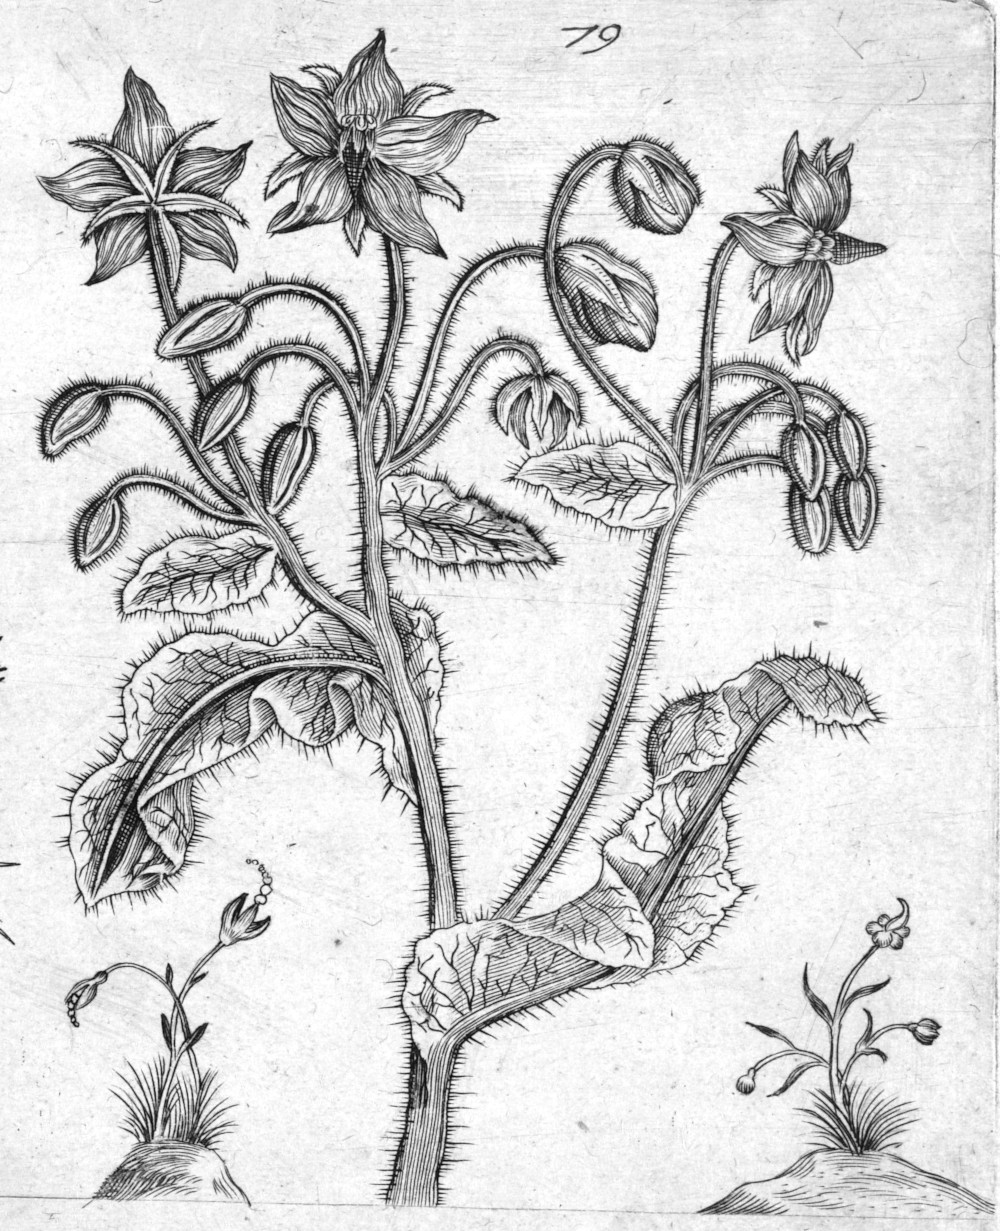
\includegraphics[keepaspectratio,width=\textwidth]{figures/borage-small.jpg}
  \captionart{Borage}
  \label{fig:borage}
\end{figure}

% Force float here
\clearpage{}

\thispagestyle{titleontop}
\subsection{Borage.}
\begin{wrapfigure}{r}{0.5\textwidth}
  \begingroup
  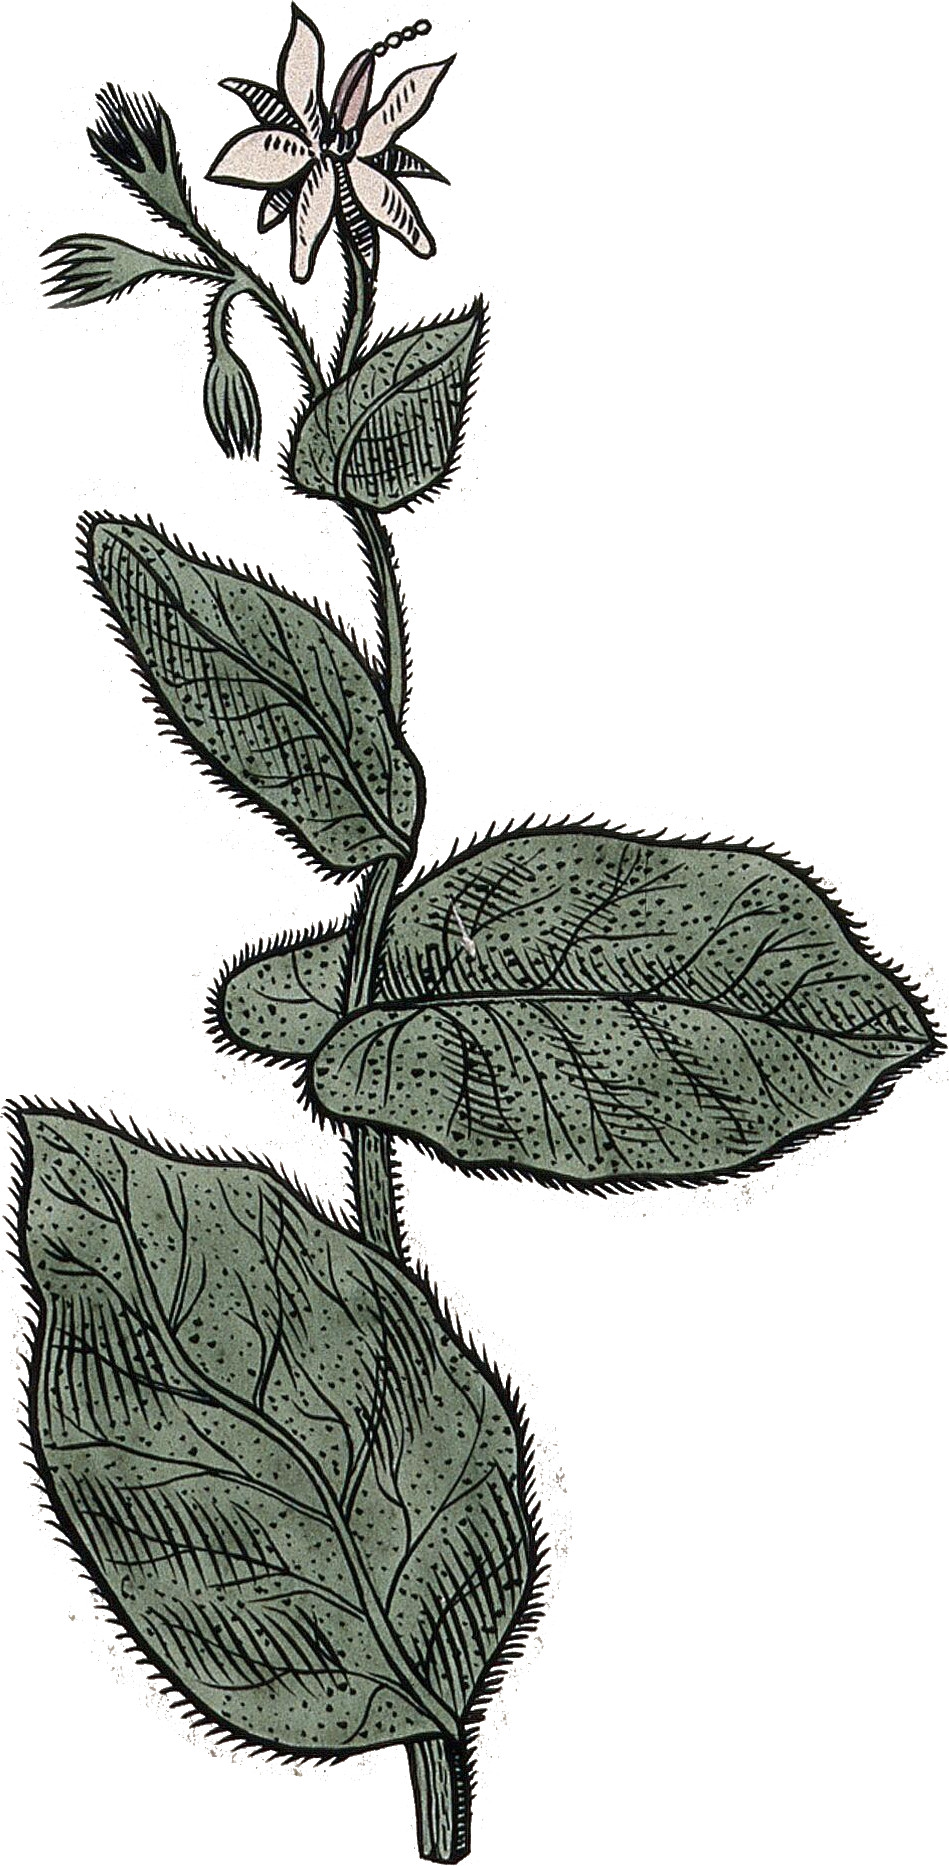
\includegraphics[keepaspectratio,width=0.5\textwidth]{figures/buglossa-small.jpg}
  \captionart{Buglosa}
  \label{fig:buglosa}
\end{wrapfigure}
In this catalogue, borage and bugloss may challenge the
chiefest place, whether in substance, juice, roots, seeds, flowers,
leaves, decoctions, distilled waters, extracts, oils, \etc{}, for such
kind of herbs be diversely varied. Bugloss is hot and moist, and
therefore worthily reckoned up amongst those herbs which expel
melancholy, and \authorfootnote{4126} exhilarate the heart, Galen, lib. 6. cap. 80. de
simpl. med. Dioscorides, lib. 4. cap. 123. Pliny much magnifies this
plant. It may be diversely used; as in broth, in \authorfootnote{4127}wine, in
conserves, syrups, \etc{}. It is an excellent cordial, and against this
malady most frequently prescribed; a herb indeed of such sovereignty,
that as Diodorus, lib. 7. bibl. Plinius, lib. 25. cap. 2. et lib. 21.
cap. 22. Plutarch, sympos. lib. 1. cap. 1. Dioscorides, lib. 5. cap.
40. Caelius, lib. 19. c. 3. suppose it was that famous Nepenthes of
\authorfootnote{4128}Homer, which Polydaenna, Thonis's wife (then king of Thebes in
Egypt), sent Helena for a token, of such rare virtue, that if taken
steeped in wine, if wife and children, father and mother, brother and
sister, and all thy dearest friends should die before thy face, thou
couldst not grieve or shed a tear for them.

Qui semel id patera mistum Nepenthes Iaccho
Hauserit, hic lachrymam, non si suavissima proles,
Si germanus ei charus, materque paterque
Oppetat, ante oculos ferro confossus atroci.

Helena's commended bowl to exhilarate the heart, had no other
ingredient, as most of our critics conjecture, than this of borage.
\subsection{Balm.}
Melissa balm hath an admirable virtue to alter melancholy, be
it steeped in our ordinary drink, extracted, or otherwise taken.
Cardan, lib. 8. much admires this herb. It heats and dries, saith
\authorfootnote{4129} Heurnius, in the second degree, with a wonderful virtue comforts
the heart, and purgeth all melancholy vapours from the spirits,
Matthiol. in lib. 3. cap. 10. in Dioscoridem. Besides they ascribe
other virtues to it, \authorfootnote{4130}as to help concoction, to cleanse the brain,
expel all careful thoughts, and anxious imaginations: the same words in
effect are in Avicenna, Pliny, Simon Sethi, Fuchsius, Leobel,
Delacampius, and every herbalist. Nothing better for him that is
melancholy than to steep this and borage in his ordinary drink.
Mathiolus, in his fifth book of Medicinal Epistles, reckons up
scorzonera, \authorfootnote{4131}not against poison only, falling sickness, and such
as are vertiginous, but to this malady; the root of it taken by itself
expels sorrow, causeth mirth and lightness of heart.

Antonius Musa, that renowned physician to Caesar Augustus, in his book
which he writ of the virtues of betony, cap. 6. wonderfully commends
that herb, animas hominum et corpora custodit, securas de metu reddit,
it preserves both body and mind, from fears, cares, griefs; cures
falling sickness, this and many other diseases, to whom Galen
subscribes, lib. 7. simp. med. Dioscorides, lib. 4. cap. 1. \etc{}.
Marigold is much approved against melancholy, and often used therefore
in our ordinary broth, as good against this and many other diseases.

\subsection{Hop.}
Lupulus, hop, is a sovereign remedy; Fuchsius, cap. 58. Plant.
hist. much extols it; \authorfootnote{4132}it purgeth all choler, and purifies the
blood. Matthiol. cap. 140. in 4. Dioscor. wonders the physicians of his
time made no more use of it, because it rarefies and cleanseth: we use
it to this purpose in our ordinary beer, which before was thick and
fulsome.

Wormwood, centaury, pennyroyal, are likewise magnified and much
prescribed (as I shall after show), especially in hypochondriac
melancholy, daily to be used, sod in whey: and as Ruffus Ephesias,
\authorfootnote{4133}Areteus relate, by breaking wind, helping concoction, many
melancholy men have been cured with the frequent use of them alone.

And because the spleen and blood are often misaffected in melancholy, I
may not omit endive, succory, dandelion, fumitory, \etc{}, which cleanse
the blood, Scolopendria, cuscuta, ceterache, mugwort, liverwort, ash,
tamarisk, genist, maidenhair, \etc{}, which must help and ease the spleen.

To these I may add roses, violets, capers, featherfew, scordium,
staechas, rosemary, ros solis, saffron, ochyme, sweet apples, wine,
tobacco, sanders, \etc{}. That Peruvian chamico, monstrosa facultate \etc{},
Linshcosteus Datura; and to such as are cold, the \authorfootnote{4134}decoction of
guiacum, China sarsaparilla, sassafras, the flowers of carduus
benedictus, which I find much used by Montanus in his Consultations,
Julius Alexandrinus, Lelius, Egubinus, and others. \authorfootnote{4135}Bernardus
Penottus prefers his herba solis, or Dutch sindaw, before all the rest
in this disease, and will admit of no herb upon the earth to be
comparable to it. It excels Homer's moly, cures this, falling sickness,
and almost all other infirmities. The same Penottus speaks of an
excellent balm out of Aponensis, which, taken to the quantity of three
drops in a cup of wine, \authorfootnote{4136}will cause a sudden alteration, drive
away dumps, and cheer up the heart. Ant. Guianerius, in his Antidotary,
hath many such. \authorfootnote{4137}Jacobus de Dondis the aggregator, repeats
ambergris, nutmegs, and allspice amongst the rest. But that cannot be
general. Amber and spice will make a hot brain mad, good for cold and
moist. Garcias ab Horto hath many Indian plants, whose virtues he much
magnifies in this disease. Lemnius, instit. cap. 58. admires rue, and
commends it to have excellent virtue, \authorfootnote{4138}to expel vain imaginations,
devils, and to ease afflicted souls. Other things are much magnified
\authorfootnote{4139}by writers, as an old cock, a ram's head, a wolf's heart borne or
eaten, which Mercurialis approves; Prosper Altinus the water of Nilus;
Gomesius all seawater, and at seasonable times to be seasick: goat's
milk, whey, \etc{}.

%SUBSECT. IV.-_Precious Stones, Metals, Minerals, Alteratives_.
\section{Precious Stones, Metals, Minerals, Alteratives.}

\lettrine{P}{recious} stones are diversely censured; many explode the use of them or
any minerals in physic, of whom Thomas Erastus is the chief, in his
tract against Paracelsus, and in an epistle of his to Peter Monavius,
\authorfootnote{4140} That stones can work any wonders, let them believe that list, no
man shall persuade me; for my part, I have found by experience there is
no virtue in them. But Matthiolus, in his comment upon
\authorfootnote{4141}Dioscorides, is as profuse on the other side, in their
commendation; so is Cardan, Renodeus, Alardus, Rueus, Encelius,
Marbodeus, \etc{}. \authorfootnote{4142}Matthiolus specifies in coral: and Oswaldus
Crollius, Basil. Chym. prefers the salt of coral. \authorfootnote{4143}Christoph.
Encelius, lib. 3. cap. 131. will have them to be as so many several
medicines against melancholy, sorrow, fear, dullness, and the like;
\authorfootnote{4144}Renodeus admires them, besides they adorn kings' crowns, grace
the fingers, enrich our household stuff, defend us from enchantments,
preserve health, cure diseases, they drive away grief, cares, and
exhilarate the mind. The particulars be these.

Granatus, a precious stone so called, because it is like the kernels of
a pomegranate, an imperfect kind of ruby, it comes from Calecut;
\authorfootnote{4145}if hung about the neck, or taken in drink, it much resisteth
sorrow, and recreates the heart. The same properties I find ascribed to
the hyacinth and topaz. \authorfootnote{4146}They allay anger, grief, diminish
madness, much delight and exhilarate the mind. \authorfootnote{4147}If it be either
carried about, or taken in a potion, it will increase wisdom, saith
Cardan, expel fear; he brags that he hath cured many madmen with it,
which, when they laid by the stone, were as mad again as ever they were
at first. Petrus Bayerus, lib. 2. cap. 13. veni mecum, Fran. Rueus,
cap. 19. de geminis, say as much of the chrysolite, \authorfootnote{4148}a friend of
wisdom, an enemy to folly. Pliny, lib. 37. Solinus, cap. 52. Albertus
de Lapid. Cardan. Encelius, lib. 3. cap. 66. highly magnifies the
virtue of the beryl, \authorfootnote{4149}it much avails to a good understanding,
represseth vain conceits, evil thoughts, causeth mirth, \etc{}. In the
belly of a swallow there is a stone found called chelidonius,
\authorfootnote{4150}which if it be lapped in a fair cloth, and tied to the right arm,
will cure lunatics, madmen, make them amiable and merry.

There is a kind of onyx called a chalcedony, which hath the same
qualities, \authorfootnote{4151}avails much against fantastic illusions which proceed
from melancholy, preserves the vigour and good estate of the whole
body.

The Eban stone, which goldsmiths use to sleeken their gold with, borne
about or given to drink, \authorfootnote{4152}hath the same properties, or not much
unlike.

Levinus Lemnius, Institui. ad vit. cap. 58. amongst other jewels, makes
mention of two more notable; carbuncle and coral, \authorfootnote{4153}which drive
away childish fears, devils, overcome sorrow, and hung about the neck
repress troublesome dreams, which properties almost Cardan gives to
that green-coloured \authorfootnote{4154}emmetris if it be carried about, or worn in a
ring; Rueus to the diamond.

Nicholas Cabeus, a Jesuit of Ferrara, in the first book of his
Magnetical Philosophy, cap. 3. speaking of the virtues of a loadstone,
recites many several opinions; some say that if it be taken in parcels
inward, si quis per frustra voret, juventutem restituet, it will, like
viper's wine, restore one to his youth; and yet if carried about them,
others will have it to cause melancholy; let experience determine.

Mercurialis admires the emerald for its virtues in pacifying all
affections of the mind; others the sapphire, which is the \authorfootnote{4155}fairest
of all precious stones, of sky colour, and a great enemy to black
choler, frees the mind, mends manners, \etc{}. Jacobus de Dondis, in his
catalogue of simples, hath ambergris, os in corde cervi, \authorfootnote{4156}the bone
in a stag's heart, a monocerot's horn, bezoar's stone \authorfootnote{4157}(of which
elsewhere), it is found in the belly of a little beast in the East
Indies, brought into Europe by Hollanders, and our countrymen
merchants. Renodeus, cap. 22. lib. 3. de ment. med. saith he saw two of
these beasts alive, in the castle of the Lord of Vitry at Coubert.

Lapis lazuli and armenus, because they purge, shall be mentioned in
their place.

Of the rest in brief thus much I will add out of Cardan, Renodeus, cap.
23. lib. 3. Rondoletius, lib. 1. de Testat. c. 15. \etc{}. \authorfootnote{4158}That
almost all jewels and precious stones have excellent virtues to pacify
the affections of the mind, for which cause rich men so much covet to
have them: \authorfootnote{4159}and those smaller unions which are found in shells
amongst the Persians and Indians, by the consent of all writers, are
very cordial, and most part avail to the exhilaration of the heart.

\subsection{Minerals.}
Most men say as much of gold and some other minerals, as
these have done of precious stones. Erastus still maintains the
opposite part. \textlatin{Disput. in Paracelsum. cap. 4. fol. 196.} he confesseth
of gold, \authorfootnote{4160} that it makes the heart merry, but in no other sense
but as it is in a miser's chest: \li{at mihi plaudo simul ac nummos
contemplor in arca}, as he said in the poet, it so revives the spirits,
and is an excellent recipe against melancholy,
%
{\gothfont
\begin{verse}
For gold in physic is a cordial,\\*
Therefore he loved gold in special.\\!
\end{verse}
}
\attrib{\getauthornote{4161} [Lines FIXME. \theeditor{}]}
%
\li{Aurum potabile}, \authorfootnote{4162}he discommends and inveighs against it, by reason
of the corrosive waters which are used in it: which argument our Dr.
Guin urgeth against D. Antonius. \authorfootnote{4163}Erastus concludes their
philosophical stones and potable gold, \etc{} to be no better than poison,
a mere imposture, a non ens; dug out of that broody hill belike this
golden stone is, ubi nascetur ridiculus mus. Paracelsus and his
chemistical followers, as so many Promethei, will fetch fire from
heaven, will cure all manner of diseases with minerals, accounting them
the only physic on the other side. \authorfootnote{4164}Paracelsus calls Galen,
Hippocrates, and all their adherents, infants, idiots, sophisters, \etc{}.
Apagesis istos qui Vulcanias istas metamorphoses sugillant, inscitiae
soboles, supinae pertinaciae alumnos, \etc{}, not worthy the name of
physicians, for want of these remedies: and brags that by them he can
make a man live 160 years, or to the world's end, with their
\authorfootnote{4165}Alexipharmacums, Panaceas, Mummias, unguentum Armarium, and such
magnetical cures, Lampas vitae et mortis, Balneum Dianae, Balsamum,
Electrum Magico-physicum, Amuleta Martialia, \etc{}. What will not he and
his followers effect? He brags, moreover, that he was primus medicorum,
and did more famous cures than all the physicians in Europe besides,
\authorfootnote{4166}a drop of his preparations should go farther than a dram, or
ounce of theirs, those loathsome and fulsome filthy potions,
heteroclitical pills (so he calls them), horse medicines, ad quoram
aspectum Cyclops Polyphemus exhorresceret. And though some condemn
their skill and magnetical cures as tending to magical superstition,
witchery, charms, \etc{}, yet they admire, stiffly vindicate nevertheless,
and infinitely prefer them. But these are both in extremes, the middle
sort approve of minerals, though not in so high a degree. Lemnius lib.
3. cap. 6. de occult. nat. mir. commends gold inwardly and outwardly
used, as in rings, excellent good in medicines; and such mixtures as
are made for melancholy men, saith Wecker, antid. spec. lib. 1. to whom
Renodeus subscribes, lib. 2. cap. 2. Ficinus, lib. 2. cap. 19. Fernel.
meth. med. lib. 5. cap. 21. de Cardiacis. Daniel Sennertus, lib. 1.
part. 2. cap. 9. Audernacus, Libavius, Quercetanus, Oswaldus Crollius,
Euvonymus, Rubeus, and Matthiolus in the fourth book of his Epistles,
Andreas a Blawen epist. ad Matthiolum, as commended and formerly used
by Avicenna, Arnoldus, and many others: \authorfootnote{4167}Matthiolus in the same
place approves of potable gold, mercury, with many such chemical
confections, and goes so far in approbation of them, that he holds
\authorfootnote{4168} no man can be an excellent physician that hath not some skill in
chemistical distillations, and that chronic diseases can hardly be
cured without mineral medicines: look for antimony among purgers.

%SUBSECT. V.-_Compound Alteratives; censure of Compounds, and mixed
\section[Compound Alteratives]{Compound Alteratives; censure of Compounds, and mixed
Physic.}

\lettrine{P}{liny}, lib. 24. c. 1, bitterly taxeth all compound medicines, \authorfootnote{4169}
Men's knavery, imposture, and captious wits, have invented those shops,
in which every man's life is set to sale: and by and by came in those
compositions and inexplicable mixtures, far-fetched out of India and
Arabia; a medicine for a botch must be had as far as the Red Sea. And
'tis not without cause which he saith; for out of question they are
much to \authorfootnote{4170}blame in their compositions, whilst they make infinite
variety of mixtures, as \authorfootnote{4171}Fuchsius notes. They think they get
themselves great credit, excel others, and to be more learned than the
rest, because they make many variations; but he accounts them fools,
and whilst they brag of their skill, and think to get themselves a
name, they become ridiculous, betray their ignorance and error. A few
simples well prepared and understood, are better than such a heap of
nonsense, confused compounds, which are in apothecaries' shops
ordinarily sold. In which many vain, superfluous, corrupt, exolete,
things out of date are to be had (saith Cornarius); a company of
barbarous names given to syrups, juleps, an unnecessary company of
mixed medicines; rudis indigestaque moles. Many times (as Agrippa
taxeth) there is by this means \authorfootnote{4172}more danger from the medicine than
from the disease, when they put together they know not what, or leave
it to an illiterate apothecary to be made, they cause death and horror
for health. Those old physicians had no such mixtures; a simple potion
of hellebore in Hippocrates' time was the ordinary purge; and at this
day, saith \authorfootnote{4173}Mat. Riccius, in that flourishing commonwealth of
China, their physicians give precepts quite opposite to ours, not
unhappy in their physic; they use altogether roots, herbs, and simples
in their medicines, and all their physic in a manner is comprehended in
a herbal: no science, no school, no art, no degree, but like a trade,
every man in private is instructed of his master. \authorfootnote{4174}Cardan cracks
that he can cure all diseases with water alone, as Hippocrates of old
did most infirmities with one medicine. Let the best of our rational
physicians demonstrate and give a sufficient reason for those intricate
mixtures, why just so many simples in mithridate or treacle, why such
and such quantity; may they not be reduced to half or a quarter?
Frustra fit per plura (as the saying is) quod fieri potest per
pauciora; 300 simples in a julep, potion, or a little pill, to what end
or purpose? I know not what \authorfootnote{4175}Alkindus, Capivaccius, Montagna, and
Simon Eitover, the best of them all and most rational, have said in
this kind; but neither he, they, nor any one of them, gives his reader,
to my judgment, that satisfaction which he ought; why such, so many
simples? Rog. Bacon hath taxed many errors in his tract de
graduationibus, explained some things, but not cleared. Mercurialis in
his book de composit. medicin. gives instance in Hamech, and Philonium
Romanum, which Hamech an Arabian, and Philonius a Roman, long since
composed, but crasse as the rest. If they be so exact, as by him it
seems they were, and those mixtures so perfect, why doth Fernelius
alter the one, and why is the other obsolete? \authorfootnote{4176}Cardan taxeth Galen
for presuming out of his ambition to correct Theriachum Andromachi, and
we as justly may carp at all the rest. Galen's medicines are now
exploded and rejected; what Nicholas Meripsa, Mesue, Celsus,
Scribanius, Actuarius, \etc{} writ of old, are most part contemned.

Mellichius, Cordus, Wecker, Quercetan, Renodeus, the Venetian,
Florentine states have their several receipts, and magistrals: they of
Nuremberg have theirs, and Augustana Pharmacopoeia, peculiar medicines
to the meridian of the city: London hers, every city, town, almost
every private man hath his own mixtures, compositions, receipts,
magistrals, precepts, as if he scorned antiquity, and all others in
respect of himself. But each man must correct and alter to show his
skill, every opinionative fellow must maintain his own paradox, be it
what it will; Delirant reges, plectuntur Achivi: they dote, and in the
meantime the poor patients pay for their new experiments, the
commonalty rue it.

Thus others object, thus I may conceive out of the weakness of my
apprehension; but to say truth, there is no such fault, no such
ambition, no novelty, or ostentation, as some suppose; but as \authorfootnote{4177}one
answers, this of compound medicines, is a most noble and profitable
invention found out, and brought into physic with great judgment,
wisdom, counsel and discretion. Mixed diseases must have mixed
remedies, and such simples are commonly mixed as have reference to the
part affected, some to qualify, the rest to comfort, some one part,
some another. Cardan and Brassavola both hold that Nullum simplex
medicamentum sine noxa, no simple medicine is without hurt or offence;
and although Hippocrates, Erasistratus, Diocles of old, in the infancy
of this art, were content with ordinary simples: yet now, saith
\authorfootnote{4178}Aetius, necessity compelleth to seek for new remedies, and to
make compounds of simples, as well to correct their harms if cold, dry,
hot, thick, thin, insipid, noisome to smell, to make them savoury to
the palate, pleasant to taste and take, and to preserve them for
continuance, by admixtion of sugar, honey, to make them last months and
years for several uses. In such cases, compound medicines may be
approved, and Arnoldus in his 18. aphorism, doth allow of it. \authorfootnote{4179}If
simples cannot, necessity compels us to use compounds; so for receipts
and magistrals, dies diem docet, one day teacheth another, and they are
as so many words or phrases, Que nunc sunt in honore vocabula si volet
usus, ebb and flow with the season, and as wits vary, so they may be
infinitely varied. Quisque suum placitum quo capiatur habet. Every man
as he likes, so many men so many minds, and yet all tending to good
purpose, though not the same way. As arts and sciences, so physic is
still perfected amongst the rest; Horae musarum nutrices, and
experience teacheth us every day \authorfootnote{4180}many things which our
predecessors knew not of. Nature is not effete, as he saith, or so
lavish, to bestow all her gifts upon an age, but hath reserved some for
posterity, to show her power, that she is still the same, and not old
or consumed. Birds and beasts can cure themselves by nature,
\authorfootnote{4181}naturae usu ea plerumque cognoscunt quae homines vix longo labore
et doctrina assequuntur, but men must use much labour and industry to
find it out. But I digress.

Compound medicines are inwardly taken, or outwardly applied. Inwardly
taken, be either liquid or solid: liquid, are fluid or consisting.

Fluid, as wines and syrups. The wines ordinarily used to this disease
are wormwood wine, tamarisk, and buglossatum, wine made of borage and
bugloss, the composition of which is specified in Arnoldus
Villanovanus, lib. de vinis, of borage, balm, bugloss, cinnamon, \etc{}.
and highly commended for its virtues: \authorfootnote{4182}it drives away leprosy,
scabs, clears the blood, recreates the spirits, exhilarates the mind,
purgeth the brain of those anxious black melancholy fumes, and
cleanseth the whole body of that black humour by urine. To which I add,
saith Villanovanus, that it will bring madmen, and such raging
bedlamites as are tied in chains, to the use of their reason again. My
conscience bears me witness, that I do not lie, I saw a grave matron
helped by this means; she was so choleric, and so furious sometimes,
that she was almost mad, and beside herself; she said, and did she knew
not what, scolded, beat her maids, and was now ready to be bound till
she drank of this borage wine, and by this excellent remedy was cured,
which a poor foreigner, a silly beggar, taught her by chance, that came
to crave an alms from door to door. The juice of borage, if it be
clarified, and drunk in wine, will do as much, the roots sliced and
steeped, \etc{} saith Ant. Mizaldus, art. med. who cities this story
verbatim out of Villanovanus, and so doth Magninus a physician of
Milan, in his regimen of health. Such another excellent compound water
I find in Rubeus de distill. sect. 3. which he highly magnifies out of
Savanarola, \authorfootnote{4183}for such as are solitary, dull, heavy or sad without
a cause, or be troubled with trembling of heart. Other excellent
compound waters for melancholy, he cites in the same place. \authorfootnote{4184}If
their melancholy be not inflamed, or their temperature over-hot.

Evonimus hath a precious aquavitae to this purpose, for such as are
cold. But he and most commend aurum potabile, and every writer
prescribes clarified whey, with borage, bugloss, endive, succory, \etc{}.
of goat's milk especially, some indefinitely at all times, some thirty
days together in the spring, every morning fasting, a good draught.

Syrups are very good, and often used to digest this humour in the
heart, spleen, liver, \etc{}. As syrup of borage (there is a famous syrup
of borage highly commended by Laurentius to this purpose in his tract
of melancholy), de pomis of king Sabor, now obsolete, of thyme and
epithyme, hops, scolopendria, fumitory, maidenhair, bizantine, \etc{}.

These are most used for preparatives to other physic, mixed with
distilled waters of like nature, or in juleps otherwise.
Consisting, are conserves or confections; conserves of borage, bugloss,
balm, fumitory, succory, maidenhair, violets, roses, wormwood, \etc{}.

Confections, treacle, mithridate, eclegms, or linctures, \etc{}. Solid, as
aromatical confections: hot, diambra, diamargaritum calidum, dianthus,
diamoschum dulce, electuarium de gemmis laetificans Galeni et Rhasis,
diagalanga, diaciminum dianisum, diatrion piperion, diazinziber,
diacapers, diacinnamonum: Cold, as diamargaritum frigidum, diacorolli,
diarrhodon abbatis, diacodion, \etc{} as every pharmacopoeia will show
you, with their tables or losings that are made out of them: with
condites and the like.

Outwardly used as occasion serves, as amulets, oils hot and cold, as of
camomile, staechados, violets, roses, almonds, poppy, nymphea,
mandrake, \etc{} to be used after bathing, or to procure sleep.
Ointments composed of the said species, oils and wax, \etc{}, as
Alablastritum Populeum, some hot, some cold, to moisten, procure sleep,
and correct other accidents.

Liniments are made of the same matter to the like purpose: emplasters
of herbs, flowers, roots, \etc{}, with oils, and other liquors mixed and
boiled together.

Cataplasms, salves, or poultices made of green herbs, pounded, or sod
in water till they be soft, which are applied to the hypochondries, and
other parts, when the body is empty.

Cerotes are applied to several parts and frontals, to take away pain,
grief, heat, procure sleep. Fomentations or sponges, wet in some
decoctions, \etc{}, epithemata, or those moist medicines, laid on linen,
to bathe and cool several parts misaffected.

Sacculi, or little bags of herbs, flowers, seeds, roots, and the like,
applied to the head, heart, stomach, \etc{}, odoraments, balls, perfumes,
posies to smell to, all which have their several uses in melancholy, as
shall be shown, when I treat of the cure of the distinct species by
themselves.

%MEMB. II.

%SUBSECT. I.-_Purging Simples upward_.
\section{Purging Simples upward.}
\lettrine{M}{elanagoga}, or melancholy purging medicines, are either simple or
compound, and that gently, or violently, purging upward or downward.
These following purge upward. \authorfootnote{4185}Asarum, or Asrabecca, which, as
Mesue saith, is hot in the second degree, and dry in the third, it is
commonly taken in wine, whey, or as with us, the juice of two or three
leaves or more sometimes, pounded in posset drink qualified with a
little liquorice, or aniseed, to avoid the fulsomeness of the taste, or
as Diaserum Fernelii. Brassivola in Catart. reckons it up amongst those
simples that only purge melancholy, and Ruellius confirms as much out
of his experience, that it purgeth \authorfootnote{4186}black choler, like hellebore
itself. Galen, lib. G. simplic. and \authorfootnote{4187}Matthiolus ascribe other
virtues to it, and will have it purge other humours as well as this.

Laurel, by Heurnius's method, ad prax. lib. 2. cap. 24. is put amongst
the strong purgers of melancholy; it is hot and dry in the fourth
degree. Dioscorides, lib. 11. cap. 114. adds other effects to it.
\authorfootnote{4188}Pliny sets down fifteen berries in drink for a sufficient potion:
it is commonly corrected with his opposites, cold and moist, as juice
of endive, purslane, and is taken in a potion to seven grains and a
half. But this and asrabecca, every gentlewoman in the country knows
how to give, they are two common vomits.

\begin{figure}[tbh]
  \begingroup
  \centering
  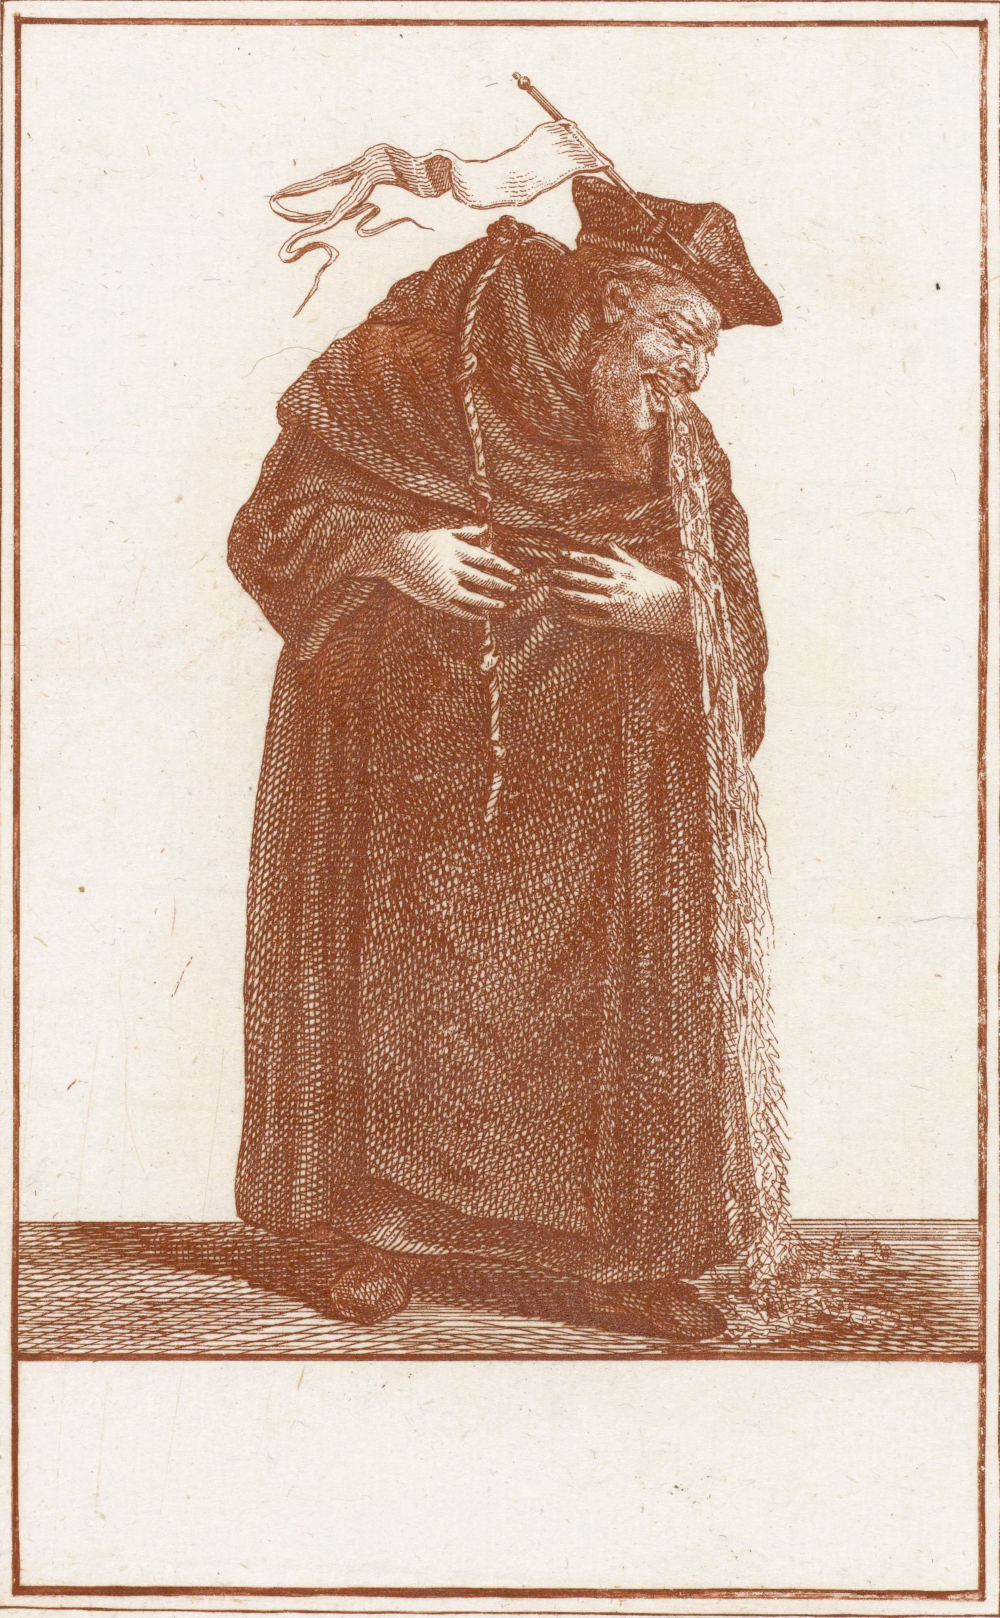
\includegraphics[keepaspectratio,width=0.5\textwidth]{figures/Vomiting-monk-Jacob-Gole-small.jpg}
  \captionart{VomitingMonk}
  \label{fig:vomitingmonk}
\end{figure}

Scilla, or sea-onion, is hot and dry in the third degree. Brassivola in
Catart. out of Mesue, others, and his own experience, will have this
simple to purge \authorfootnote{4189}melancholy alone. It is an ordinary vomit, vinum
scilliticum mixed with rubel in a little white wine.

White hellebore, which some call sneezing-powder, a strong purger
upward, which many reject, as being too violent: Mesue and Averroes
will not admit of it, \authorfootnote{4190}by reason of danger of suffocation,
\authorfootnote{4191}great pain and trouble it puts the poor patient to, saith
Dodonaeus. Yet Galen, lib. 6. simpl. med. and Dioscorides, cap. 145.
allow of it. It was indeed \authorfootnote{4192} terrible in former times, as Pliny
notes, but now familiar, insomuch that many took it in those days,
\authorfootnote{4193}that were students, to quicken their wits, which Persius Sat. 1.
objects to Accius the poet, Illas Acci ebria veratro. \authorfootnote{4194}It helps
melancholy, the falling sickness, madness, gout, \etc{}, but not to be
taken of old men, youths, such as are weaklings, nice, or effeminate,
troubled with headache, high-coloured, or fear strangling, saith
Dioscorides. \authorfootnote{4195}Oribasius, an old physician, hath written very
copiously, and approves of it, in such affections which can otherwise
hardly be cured. Hernius, lib. 2. prax. med. de vomitoriis, will not
have it used \authorfootnote{4196}but with great caution, by reason of its strength,
and then when antimony will do no good, which caused Hermophilus to
compare it to a stout captain (as Codroneus observes cap. 7. comment.
de Helleb.) that will see all his soldiers go before him and come post
principia, like the bragging soldier, last himself; \authorfootnote{4197}when other
helps fail in inveterate melancholy, in a desperate case, this vomit is
to be taken. And yet for all this, if it be well prepared, it may be
\authorfootnote{4198} securely given at first. \authorfootnote{4199}Matthiolus brags, that he hath
often, to the good of many, made use of it, and Heurnius, \authorfootnote{4200}that he
hath happily used it, prepared after his own prescript, and with good
success. Christophorus a Vega, lib. 3. c. 41, is of the same opinion,
that it may be lawfully given; and our country gentlewomen find it by
their common practice, that there is no such great danger in it. Dr.
Turner, speaking of this plant in his Herbal, telleth us, that in his
time it was an ordinary receipt among good wives, to give hellebore in
powder to ii'd weight, and he is not much against it. But they do
commonly exceed, for who so bold as blind Bayard, and prescribe it by
pennyworths, and such irrational ways, as I have heard myself market
folks ask for it in an apothecary's shop: but with what success God
knows; they smart often for their rash boldness and folly, break a
vein, make their eyes ready to start out of their heads, or kill
themselves. So that the fault is not in the physic, but in the rude and
indiscreet handling of it. He that will know, therefore, when to use,
how to prepare it aright, and in what dose, let him read Heurnius lib.
2. prax. med. Brassivola de Catart. Godefridus Stegius the emperor
Rudolphus' physician, cap. 16. Matthiolus in Dioscor. and that
excellent commentary of Baptista Codroncus, which is instar omnium de
Helleb. alb. where we shall find great diversity of examples and
receipts.

Antimony or stibium, which our chemists so much magnify, is either
taken in substance or infusion, \etc{}, and frequently prescribed in this
disease. It helps all infirmities, saith \authorfootnote{4201}Matthiolus, which
proceed from black choler, falling sickness, and hypochondriacal
passions; and for farther proof of his assertion, he gives several
instances of such as have been freed with it: \authorfootnote{4202}one of Andrew
Gallus, a physician of Trent, that after many other essays, imputes the
recovery of his health, next after God, to this remedy alone. Another
of George Handshius, that in like sort, when other medicines failed,
\authorfootnote{4203}was by this restored to his former health, and which of his
knowledge others have likewise tried, and by the help of this admirable
medicine, been recovered. A third of a parish priest at Prague in
Bohemia, \authorfootnote{4204}that was so far gone with melancholy, that he doted, and
spake he knew not what; but after he had taken twelve grains of
stibium, (as I myself saw, and can witness, for I was called to see
this miraculous accident) he was purged of a deal of black choler, like
little gobbets of flesh, and all his excrements were as black blood (a
medicine fitter for a horse than a man), yet it did him so much good,
that the next day he was perfectly cured. This very story of the
Bohemian priest, Sckenkius relates verbatim, Exoter. experiment. ad.
var. morb. cent. 6. observ. 6. with great approbation of it. Hercules
de Saxonia calls it a profitable medicine, if it be taken after meat to
six or eight grains, of such as are apt to vomit. Rodericus a Fonseca
the Spaniard, and late professor of Padua in Italy, extols it to this
disease, Tom. 2. consul. 85. so doth Lod. Mercatus de inter. morb. cur.
lib. 1. cap. 17. with many others. Jacobus Gervinus a French physician,
on the other side, lib. 2. de venemis confut. explodes all this, and
saith he took three grains only upon Matthiolus and some others'
commendation, but it almost killed him, whereupon he concludes,
\authorfootnote{4205}antimony is rather poison than a medicine. Th. Erastus concurs
with him in his opinion, and so doth \AE{}lian Montaltus cap. 30 de melan.

But what do I talk? 'tis the subject of whole books; I might cite a
century of authors pro and con. I will conclude with \authorfootnote{4206}Zuinger,
antimony is like Scanderbeg's sword, which is either good or bad,
strong or weak, as the party is that prescribes, or useth it: a worthy
medicine if it be rightly applied to a strong man, otherwise poison.

For the preparing of it, look in Evonimi thesaurus, Quercetan, Oswaldus
Crollius, Basil. Chim. Basil. Valentius, \etc{}.

Tobacco, divine, rare, superexcellent tobacco, which goes far beyond
all the panaceas, potable gold, and philosopher's stones, a sovereign
remedy to all diseases. A good vomit, I confess, a virtuous herb, if it
be well qualified, opportunely taken, and medicinally used; but as it
is commonly abused by most men, which take it as tinkers do ale, 'tis a
plague, a mischief, a violent purger of goods, lands, health, hellish,
devilish and damned tobacco, the ruin and overthrow of body and soul.

%SUBSECT. II.-_Simples purging Melancholy downward_.
\section{Simples purging Melancholy downward.}

\lettrine{P}{olypody} and epithyme are, without all exceptions, gentle purgers of
melancholy. Dioscorides will have them void phlegm; but Brassivola out
of his experience averreth, that they purge this humour; they are used
in decoction, infusion, \etc{} simple, mixed, \etc{}.

Mirabolanes, all five kinds, are happily \authorfootnote{4207}prescribed against
melancholy and quartan agues; Brassivola speaks out \authorfootnote{4208}of a thousand
experiences, he gave them in pills, decoctions, \etc{}, look for peculiar
receipts in him.

Stoechas, fumitory, dodder, herb mercury, roots of capers, genista or
broom, pennyroyal and half-boiled cabbage, I find in this catalogue of
purgers of black choler, origan, featherfew, ammoniac \authorfootnote{4209}salt,
saltpetre. But these are very gentle; alyppus, dragon root, centaury,
ditany, colutea, which Fuchsius cap. 168 and others take for senna, but
most distinguish. Senna is in the middle of violent and gentle purgers
downward, hot in the second degree, dry in the first. Brassivola calls
it \authorfootnote{4210}a wonderful herb against melancholy, it scours the blood,
lightens the spirits, shakes off sorrow, a most profitable medicine, as
\authorfootnote{4211} Dodonaeus terms it, invented by the Arabians, and not heard of
before. It is taken diverse ways, in powder, infusion, but most
commonly in the infusion, with ginger, or some cordial flowers added to
correct it. Actuarius commends it sodden in broth, with an old cock, or
in whey, which is the common conveyor of all such things as purge black
choler; or steeped in wine, which Heurnius accounts sufficient, without
any farther correction.

Aloes by most is said to purge choler, but Aurelianus lib. 2. c. 6. de
morb. chron. Arculanus cap. 6. in 9. Rhasis Julius Alexandrinus,
consil. 185. Scoltz. Crato consil 189. Scoltz. prescribe it to this
disease; as good for the stomach and to open the haemorrhoids, out of
Mesue, Rhasis, Serapio, Avicenna: Menardus ep. lib. 1. epist. 1.
opposeth it, aloes \authorfootnote{4212}doth not open the veins, or move the
haemorrhoids, which Leonhartus Fuchsius paradox. lib. 1. likewise
affirms; but Brassivola and Dodonaeus defend Mesue out of their
experience; let \authorfootnote{4213}Valesius end the controversy.

Lapis armenus and lazuli are much magnified by \authorfootnote{4214}Alexander lib. 1.
cap. 16. Avicenna, Aetius, and Actuarius, if they be well washed, that
the water be no more coloured, fifty times some say. \authorfootnote{4215}That good
Alexander (saith Guianerus) puts such confidence in this one medicine,
that he thought all melancholy passions might be cured by it; and I for
my part have oftentimes happily used it, and was never deceived in the
operation of it. The like may be said of lapis lazuli, though it be
somewhat weaker than the other. Garcias ab Horto, hist. lib. 1. cap.
65. relates, that the \authorfootnote{4216}physicians of the Moors familiarly
prescribe it to all melancholy passions, and Matthiolus ep. lib. 3.
\authorfootnote{4217}brags of that happy success which he still had in the
administration of it. Nicholas Meripsa puts it amongst the best
remedies, sect. 1. cap. 12. in Antidotis; \authorfootnote{4218}and if this will not
serve (saith Rhasis) then there remains nothing but lapis armenus and
hellebore itself. Valescus and Jason Pratensis much commend pulvis
hali, which is made of it. James Damascen. 2. cap. 12. Hercules de
Saxonia, \etc{}, speaks well of it. Crato will not approve this; it and
both hellebores, he saith, are no better than poison. Victor
Trincavelius, lib. 2. cap. 14, found it in his experience, \authorfootnote{4219}to be
very noisome, to trouble the stomach, and hurt their bodies that take
it overmuch.
\clearpage{}

\subsection{Black hellebore}
\begin{wrapfigure}{r}{0.4\textwidth}
  \begingroup
  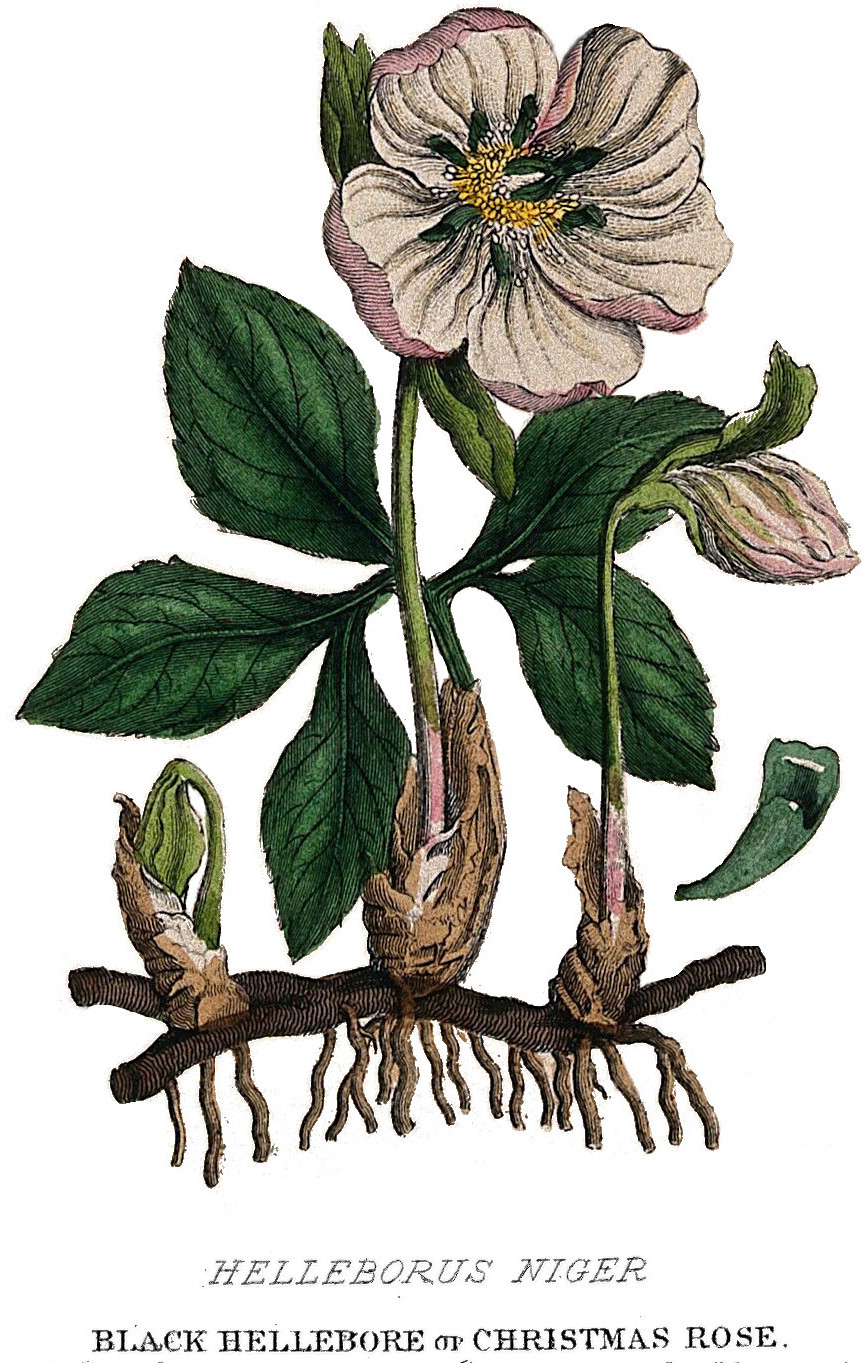
\includegraphics[keepaspectratio,width=0.4\textwidth]{figures/Helleborus-Niger-small.jpg}
  \captionart{HelleborusNiger2}
  \label{fig:helleborusniger2}
\end{wrapfigure}
Black hellebore, that most renowned plant, and famous purger of
melancholy, which all antiquity so much used and admired, was first
found out by Melanpodius a shepherd, as Pliny records, lib. 25. cap. 5.
\authorfootnote{4220}who, seeing it to purge his goats when they raved, practised it
upon Elige and Calene, King Praetus' daughters, that ruled in Arcadia,
near the fountain Clitorius, and restored them to their former health.

In Hippocrates's time it was in only request, insomuch that he writ a
book of it, a fragment of which remains yet. Theophrastus, \authorfootnote{4221}Galen,
Pliny, Caelius Aurelianus, as ancient as Galen, lib. 1, cap. 6. Aretus
lib. 1. cap. 5. Oribasius lib. 7. collect. a famous Greek, Aetius ser.
3. cap. 112 \& 113 p. Aegineta, Galen's Ape, lib. 7. cap. 4. Actuarius,
Trallianus lib. 5. cap. 15. Cornelius Celsus only remaining of the old
Latins, lib. 3. cap. 23, extol and admire this excellent plant; and it
was generally so much esteemed of the ancients for this disease amongst
the rest, that they sent all such as were crazed, or that doted, to the
Anticyrae, or to Phocis in Achaia, to be purged, where this plant was
in abundance to be had. In Strabo's time it was an ordinary voyage,
Naviget Anticyras; a common proverb among the Greeks and Latins, to bid
a dizzard or a mad man go take hellebore; as in Lucian, Menippus to
Tantalus, Tantale desipis, helleboro epoto tibi opus est, eoque sane
meraco, thou art out of thy little wit, O Tantalus, and must needs
drink hellebore, and that without mixture. Aristophanes in Vespis,
drink hellebore, \etc{} and Harpax in the \authorfootnote{4222} Comoedian, told Simo and
Ballio, two doting fellows, that they had need to be purged with this
plant. When that proud Menacrates \textgreek{ὀ ζεὺς}, had writ an arrogant letter
to Philip of Macedon, he sent back no other answer but this, Consulo
tibi ut ad Anticyram te conferas, noting thereby that he was crazed,
atque ellebore indigere, had much need of a good purge. Lilius Geraldus
saith, that Hercules, after all his mad pranks upon his wife and
children, was perfectly cured by a purge of hellebore, which an
Anticyrian administered unto him. They that were sound commonly took it
to quicken their wits, (as Ennis of old, \authorfootnote{4223}Qui non nisi potus ad
arma-prosiluit dicenda, and as our poets drink sack to improve their
inventions (I find it so registered by Agellius lib. 17. cap. 15.)
%\begin{figure}[H]
%  \begingroup
%  \centering
%  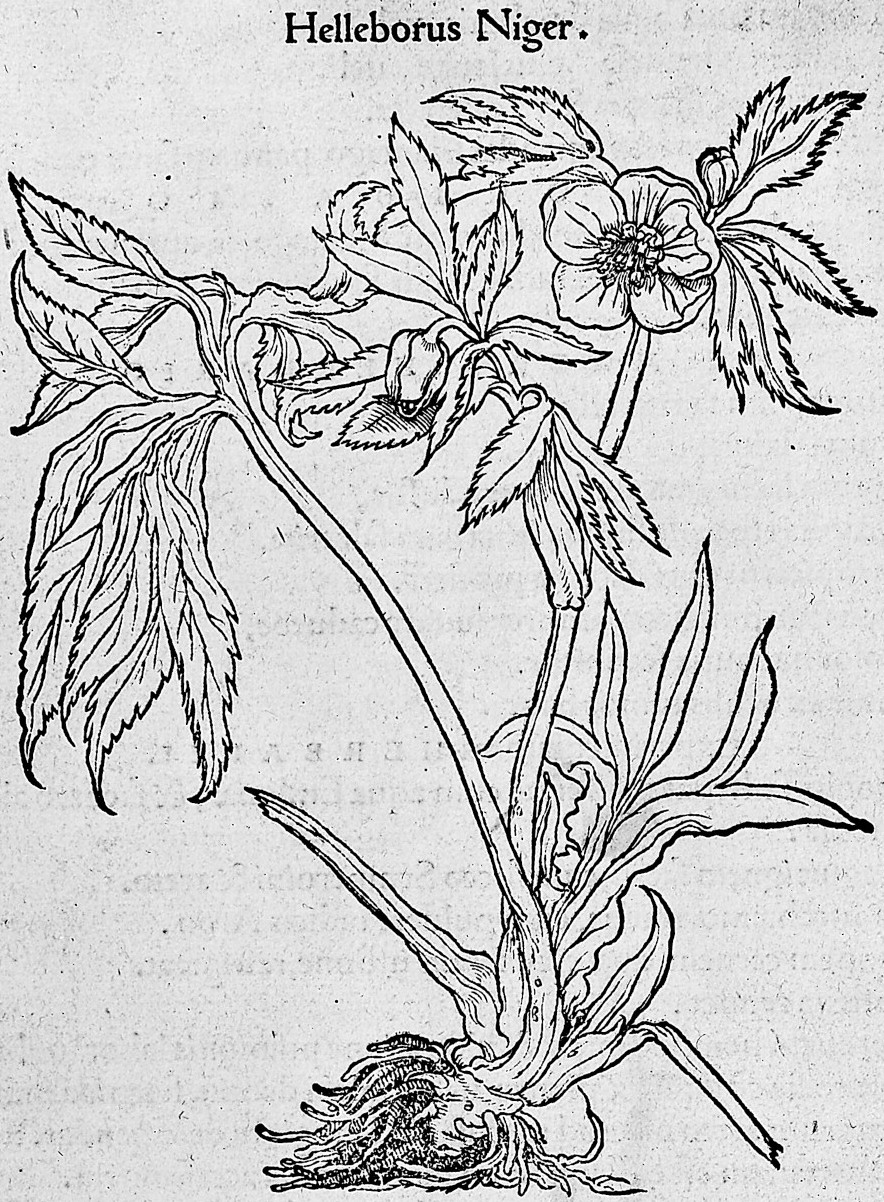
\includegraphics[keepaspectratio,width=\textwidth]{figures/HelleborusNiger-small}
%  \captionart{HelleborusNiger}
%  \label{fig:helleborusniger}
%\end{figure}

Cameades the academic, when he was to write against Zeno the stoic,
purged himself with hellebore first, which \authorfootnote{4224}Petronius puts upon
Chrysippus. In such esteem it continued for many ages, till at length
Mesue and some other Arabians began to reject and reprehend it, upon
whose authority for many following lustres, it was much debased and
quite out of request, held to be poison and no medicine; and is still
oppugned to this day by \authorfootnote{4225} Crato and some junior physicians. Their
reasons are, because Aristotle l. 1. de plant. c. 3. said, henbane and
hellebore were poison; and Alexander Aphrodiseus, in the preface of his
problems, gave out, that (speaking of hellebore) \authorfootnote{4226}Quails fed on
that which was poison to men. Galen. l. 6. Epid. com. 5. Text. 35.
confirms as much: \authorfootnote{4227}Constantine the emperor in his Geoponicks,
attributes no other virtue to it, than to kill mice and rats, flies and
mouldwarps, and so Mizaldus, Nicander of old, Gervinus, Sckenkius, and
some other Neoterics that have written of poisons, speak of hellebore
in a chief place. 

Nicholas Leonicus hath a story of Solon\authorfootnote{4228}, that
besieging, I know not what city, steeped hellebore in a spring of
water, which by pipes was conveyed into the middle of the town, and so
either poisoned, or else made them so feeble and weak by purging, that
they were not able to bear arms. Notwithstanding all these cavils and
objections, most of our late writers do much approve of it. \authorfootnote{4229}
Gariopontus lib. 1. cap. 13. Codronchus com. de helleb. Fallopius lib.
de med. purg. simpl. cap. 69. et consil. 15. Trincavelii, Montanus 239.
Frisemelica consil. 14. Hercules de Saxonia, so that it be opportunely
given. Jacobus de Dondis, Agg. Amatus, Lucet. cent. 66. Godef. Stegius
cap. 13. Hollerius, and all our herbalists subscribe. Fernelius meth.
med. lib. 5. cap. 16. confesseth it to be a \authorfootnote{4230} terrible purge and
hard to take, yet well given to strong men, and such as have able
bodies. P. Forestus and Capivaccius forbid it to be taken in substance,
but allow it in decoction or infusion, both which ways P. Monavius
approves above all others, Epist. 231. Scoltzii, Jacchinus in 9.
Rhasis, commends a receipt of his own preparing; Penottus another of
his chemically prepared, Evonimus another. Hildesheim spicel. 2. de
mel. hath many examples how it should be used, with diversity of
receipts. Heurnius lib. 7. prax. med. cap. 14. calls it an
\authorfootnote{4231}innocent medicine howsoever, if it be well prepared. The root of
it is only in use, which may be kept many years, and by some given in
substance, as by Fallopius and Brassivola amongst the rest, who
\authorfootnote{4232}brags that he was the first that restored it again to its use,
and tells a story how he cured one Melatasta, a madman, that was
thought to be possessed, in the Duke of Ferrara's court, with one purge
of black hellebore in substance: the receipt is there to be seen; his
excrements were like ink, \authorfootnote{4233}he perfectly healed at once; Vidus
Vidius, a Dutch physician, will not admit of it in substance, to whom
most subscribe, but as before, in the decoction, infusion, or which is
all in all, in the extract, which he prefers before the rest, and calls
suave medicamentum, a sweet medicine, an easy, that may be securely
given to women, children, and weaklings. Baracellus, horto geniali,
terms it maximae praestantia medicamentum, a medicine of great worth
and note. Quercetan in his Spagir Phar. and many others, tell wonders
of the extract. Paracelsus, above all the rest, is the greatest admirer
of this plant; and especially the extract, he calls it Theriacum,
terrestre Balsamum, another treacle, a terrestrial balm, instar omnium,
all in all, the \authorfootnote{4234}sole and last refuge to cure this malady, the
gout, epilepsy, leprosy, \etc{}. If this will not help, no physic in the
world can but mineral, it is the upshot of all. Matthiolus laughs at
those that except against it, and though some abhor it out of the
authority of Mesue, and dare not adventure to prescribe it, \authorfootnote{4235}yet I
(saith he) have happily used it six hundred times without offence, and
communicated it to diverse worthy physicians, who have given me great
thanks for it. Look for receipts, dose, preparation, and other cautions
concerning this simple, in him, Brassivola, Baracelsus, Codronchus, and
the rest.

%SUBSECT. III.-_Compound Purgers_.
\section{Compound Purgers.}

\lettrine{C}{ompound} medicines which purge melancholy, are either taken in the
superior or inferior parts: superior at mouth or nostrils. At the mouth
swallowed or not swallowed: If swallowed liquid or solid: liquid, as
compound wine of hellebore, scilla or sea-onion, senna, Vinum
Scilliticum, Helleboratum, which \authorfootnote{4236}Quercetan so much applauds for
melancholy and madness, either inwardly taken, or outwardly applied to
the head, with little pieces of linen dipped warm in it. Oxymel.
Scilliticum, Syrupus Helleboratus major and minor in Quercetan, and
Syrupus Genistae for hypochondriacal melancholy in the same author,
compound syrup of succory, of fumitory, polypody, \etc{}. Heurnius his
purging cock-broth. Some except against these syrups, as appears by
\authorfootnote{4237}Udalrinus Leonoras his epistle to Matthiolus, as most pernicious,
and that out of Hippocrates, cocta movere, et medicari, non cruda, no
raw things to be used in physic; but this in the following epistle is
exploded and soundly confuted by Matthiolus: many juleps, potions,
receipts, are composed of these, as you shall find in Hildesheim
spicel. 2. Heurnius lib. 2. cap. 14. George Sckenkius Ital. med. prax.
\etc{}.

Solid purges are confections, electuaries, pills by themselves, or
compound with others, as de lapide lazulo, armeno, pil. indae, of
fumitory, \etc{}. Confection of Hamech, which though most approve,
Solenander sec. 5. consil. 22. bitterly inveighs against, so doth
Rondoletius Pharmacop. officina, Fernelius and others; diasena,
diapolypodium, diacassia, diacatholicon, Wecker's electuary de
Epithymo, Ptolemy's hierologadium, of which diverse receipts are daily
made.

Aetius 22. 23. commends Hieram Ruffi. Trincavelius consil. 12. lib. 4.
approves of hiera; non, inquit, invenio melius medicamentum, I find no
better medicine, he saith. Heurnius adds pil. aggregat. pills de
Epithymo. pil. Ind. Mesue describes in the Florentine Antidotary,
Pilulae sine quibus esse nolo, Pilulae, Cochics, cum Helleboro, Pil.
Arabicae, Faetida, de quinque generibus mirabolanorum, \etc{}. More proper
to melancholy, not excluding in the meantime, turbith, manna, rhubarb,
agaric, elescophe, \etc{} which are not so proper to this humour. For, as
Montaltus holds cap. 30. and Montanus cholera etiam purganda, quod
atrae, sit pabulum, choler is to be purged because it feeds the other:
and some are of an opinion, as Erasistratus and Asclepiades maintained
of old, against whom Galen disputes, \authorfootnote{4238}that no physic doth purge
one humour alone, but all alike or what is next. Most therefore in
their receipts and magistrals which are coined here, make a mixture of
several simples and compounds to purge all humours in general as well
as this. Some rather use potions than pills to purge this humour,
because that as Heurnius and Crato observe, hic succus a sicco remedio
agre trahitur, this juice is not so easily drawn by dry remedies, and
as Montanus adviseth 25 cons. All \authorfootnote{4239}drying medicines are to be
repelled, as aloe, hiera, and all pills whatsoever, because the disease
is dry of itself.

I might here insert many receipts of prescribed potions, boles, \etc{}. The
doses of these, but that they are common in every good physician, and
that I am loath to incur the censure of Forestus, lib. 3. cap. 6. de
urinis, \authorfootnote{4240}against those that divulge and publish medicines in their
mother-tongue, and lest I should give occasion thereby to some ignorant
reader to practise on himself, without the consent of a good physician.

Such as are not swallowed, but only kept in the mouth, are gargarisms
used commonly after a purge, when the body is soluble and loose. Or
apophlegmatisms, masticatories, to be held and chewed in the mouth,
which are gentle, as hyssop, origan, pennyroyal, thyme, mustard;
strong, as pellitory, pepper, ginger, \etc{}.

Such as are taken into the nostrils, errhina are liquid or dry, juice
of pimpernel, onions, \etc{}, castor, pepper, white hellebore, \etc{}. To
these you may add odoraments, perfumes, and suffumigations, \etc{}.

Taken into the inferior parts are clysters strong or weak,
suppositories of Castilian soap, honey boiled to a consistence; or
stronger of scammony, hellebore, \etc{}.

These are all used, and prescribed to this malady upon several
occasions, as shall be shown in its place.

%MEMB. III.

\section{Chirurgical Remedies.}

\lettrine[lines=3]{I}{n} letting of blood three main circumstances are to be considered,
\authorfootnote{4241} Who, how much, when. That is, that it be done to such a one as
may endure it, or to whom it may belong, that he be of a competent age,
not too young, nor too old, overweak, fat, or lean, sore laboured, but
to such as have need, are full of bad blood, noxious humours, and may
be eased by it.

The quantity depends upon the party's habit of body, as he is strong or
weak, full or empty, may spare more or less.

In the morning is the fittest time: some doubt whether it be best
fasting, or full, whether the moon's motion or aspect of planets be to
be observed; some affirm, some deny, some grant in acute, but not in
chronic diseases, whether before or after physic. 'Tis Heurnius'
aphorism a phlebotomia auspicandum esse curiationem, non a pharmacia,
you must begin with bloodletting and not physic; some except this
peculiar malady. But what do I? Horatius Augenius, a physician of
Padua, hath lately writ 17 books of this subject, Jobertus, \etc{}.

Particular kinds of bloodletting in use \authorfootnote{4242}are three, first is that
opening a vein in the arm with a sharp knife, or in the head, knees, or
any other parts, as shall be thought fit.

Cupping-glasses with or without scarification, ocyssime compescunt,
saith Fernelius, they work presently, and are applied to several parts,
to divert humours, aches, winds, \etc{}.

Horseleeches are much used in melancholy, applied especially to the
haemorrhoids. Horatius Augenius, lib. 10. cap. 10. Platerus de mentis
alienat. cap. 3. Altomarus, Piso, and many others, prefer them before
any evacuations in this kind.

\authorfootnote{4243}Cauteries, or searing with hot irons, combustions, borings,
lancings, which, because they are terrible, Dropax and Sinapismus are
invented by plasters to raise blisters, and eating medicines of pitch,
mustard-seed, and the like.

Issues still to be kept open, made as the former, and applied in and to
several parts, have their use here on diverse occasions, as shall be
shown.
}
